%---PACKAGES----------------------------------------
\documentclass[a4paper,11pt]{report}

\usepackage{import}
\import{Packages/}{custom_packages.tex}
\import{Packages/}{custom_macros.tex}


% DOCUMENT -------------------------

\begin{document}

\begin{titlepage}

    \center
    
    \textsc{\LARGE Université Libre de Bruxelles}\\[1.5cm]
    
\includegraphics[scale=.1]{Pictures/background.png}\\[0.5cm]
    \textsc{\large PHYS-F432}\\[0.5cm]
    
    
    \HRule \\[0.6cm]
    {\huge \bfseries Théorie de la gravitation}\\[0.4cm]
    \HRule \\[1.5cm]
    
    
    \begin{minipage}{0.4\textwidth}
    \begin{center} \large
    Louan \textsc{Mol}
    \end{center}
    
    \end{minipage}\\[8cm]
    
    {\large 2019-2020}\\[2cm]
    
    \vfill

\end{titlepage}

\nocite{weinberg}
\nocite{wheeler}
\nocite{hawking}
\nocite{hartle}
\nocite{price}
\nocite{nakahara}
\nocite{wald}
\nocite{lee}
\nocite{gutt}

\chapter*{Avant-propos}

    Ce document reprend mes notes du cours de \textit{Théorie de la gravitation} donné par le professeur \textit{F. Ferrari} à l'\textit{Université Libre de Bruxelles (ULB)} durant l'année 2019-2020. Ce cours est destiné aux étudiants en première année de master en physique. Je me suis permis de rajouter certains détails, rappels et applications trouvés dans les différentes références.\\
    
    Les notions mathématiques sont définies le plus rigoureusement possible, tout en y apportant une interprétation physique. Le but étant d'avoir un fondement mathématique solide. Beaucoup de notations et de définitions sont tirées du cours de Géométrie Différentielle de \textit{S. Gutt}. \\
    
    Je n'ai pas la prétention de faire de ce document une référence, le but est simplement de transcrire mes notes sous une forme qui m'est agréable.\\
    
    Merci à \textit{Guillaume Houyoux} et à \textit{Eliott Van Steirteghem} pour les schémas ainsi que pour leurs relectures attentives. Pour les fautes qui nous aurons échappées, vous pouvez me contacter via mon adresse mail : \verb?louamol@ulb.ac.be?.\\
    
    %Merci à \texit{A. Fiorucci} pour les corrections des exercices et les discussions sur le cours qui ont grandement contribué à l'amélioration des ces notes.

\printbibliography[title=Références]
\pagebreak
\tableofcontents
\pagebreak

\chapter{Introduction}

    \section*{Notations}
    
        Nous utilisons la \textit{convention de sommation d'Einstein} pour les indices répétés de variances différentes. Les indices grecs prennent les valeurs $0,1,\dots,n-1$ et les indices romains prennent les valeurs $1,\dots,n-1$ où $n$ est la dimension.

    \section{Interactions fondamentales}
    
        Historiquement, il est apparut qu'il y a quatre interactions fondamentales dans la nature : les interactions nucléaires forte et faible, l'interaction électromagnétique et l'interaction gravitationnelle. Les interactions nucléaires ont toutes les deux une faible portée, de l'ordre du fermi ($\sim10^{-15}\meter$), alors que  l'électromagnétisme et la gravitation semblent avoir une portée infinie. De par leur nature, les interactions nucléaires sont essentiellement décrites dans des théories quantiques alors que les deux dernières peuvent être décrites de manière classique. L'électromagnétisme ayant certains effets quantiques, nous pouvons les décrire via l'électrodynamique quantique (QED). Au cours du $20^{\text{ème}}$ siècle, il a été découvert que l'interaction nucléaire faible et l'électromagnétisme pouvaient être vues comme deux faces d'une même pièce : l'interaction électrofaible.\\
        
        L'interaction gravitationnelle se distingue des autres à plusieurs niveaux. Premièrement, la gravitation est une interaction extrêmement faible par rapport aux autres. Pour illustrer cela, imaginons deux électrons séparés d'une distance $r$. Comparons les ordres de grandeur de l'interaction gravitationnelle et de l'interaction électromagnétique, on voit que
        \begin{equation}
            \abs{\frac{F_{\text{grav}}}{F_{\text{é-m}}}} = \frac{Gm^2}{r^2}\frac{4\pi\varepsilon_0r^2}{q^2} = \frac{4\pi\varepsilon_0 m^2}{q^2} \approx 2,4\cdot10^{-43}
        \end{equation}
        où $m$ est la masse d'un électron. Ce résultat est indépendant de la distance qui sépare les électrons. La force gravitationnelle est donc négligeable au niveau microscopique. Deuxièmement, à l'inverse des autres interactions, la gravité est uniquement cumulative car toutes les masses sont positives, il n'y a donc pas d'effet d'écrantage. Pour l'électromagnétisme par exemple, il y a des charges positives et négatives ce qui permet à la matière d'être électriquement neutre, ce n'est pas le cas pour la gravitation.\\
        
        On dit que la théorie newtonnienne de la gravitation est une théorie classique car elle n'est pas invariante par la relativité einsteinienne (relativité restreinte) mais juste sous le groupe de relativité galiléenne. Il semble important au niveau conceptuel de mettre au point une théorie relativiste de la gravitation. Nous verrons plus tard que cette théorie permet également d'expliquer un grand nombre de phénomènes qui ne sont pas expliqués par la théorie de Newton (avancée du périhélie de Mercure, lentilles gravitationnelles,...). Plus encore, elle permet de prédire l'existence de phénomènes dont nous n'avions pas idée de l'existence (trous noirs, trous de ver, ondes gravitationnelles, ...).\\
        
        A ce stade, nous pouvons nous demander quel ordre de grandeur les effets d'une telle théorie auraient. Soient $\O$ une observable quelconque, $\O_{\text{Newton}}$ la valeur prédite par la théorie de Newton et $\O_{\text{rela}}$ la valeur prédite par une théorie relativiste. Dans ce cas,
        \begin{equation}
            \O_{\text{rela}} = (1+\alpha)\O_{\text{Newton}}
        \end{equation}
        où $\alpha$ est un terme de correction sans dimension. Si les grandeurs importantes de notre situation sont uniquement la masse $M$, la constante gravitationnelle $G$, une distance $R$ et la vitesse de la lumière $c$, la seule combinaison sans dimension possible de ces grandeurs est 
        \begin{equation}
            \varepsilon~\hat{=}~\frac{GM}{Rc^2}.
        \end{equation}
        On peut donc s'attendre à ce que les corrections soient proportionnelles à $\varepsilon$ (ou à n'importe quelle puissance de $\varepsilon$).
        \begin{equation}
            \alpha\sim\varepsilon+\O(\varepsilon^2)
        \end{equation}
        On distingue deux régimes :
        \begin{itemize}[label=\textbullet]
            \item $\varepsilon\ll 1$ : les effets relativistes sont négligeables
            \item $\varepsilon\sim 1$ : les effets relativistes jouent un rôle important
        \end{itemize}
        Ce raisonnement rapide n'est pas rigoureux mais il permet de se convaincre que les effets d'une théorie relativiste de la gravitation seraient tout à fait observables. 
        \begin{exmp}
            Pour le soleil,
            \begin{align*}
                M_\odot &= 2,0\cdot10^{30}\kilo\gram \\
                R_\odot &= 7,0\cdot10^{5}\kilo\meter
            \end{align*}
            et donc
            \begin{equation}
                \varepsilon_\odot  = \frac{GM_\odot}{R_\odot c^2}\sim 10^{-6}.
            \end{equation}
            Les observatoires astronomiques actuels permettent de mesurer ce genre de facteurs jusqu'à cinq chiffres significatifs. 
        \end{exmp}
        \begin{exmp}
            Pour la Terre,
            \begin{align*}
                M_\oplus &= 6,0\cdot10^{24}\kilo\gram \\
                R_\oplus &= 6,4\cdot10^{3}\kilo\meter
            \end{align*}
            et donc
            \begin{equation}
                \varepsilon_\oplus = \frac{GM_\oplus}{R_\oplus c^2}\sim 10^{-9}.
            \end{equation}
        \end{exmp}
        \begin{exmp}
            Pour l'univers,
            \begin{align*}
                M &= 3\cdot10^{52}\kilo\gram \\
                R &= 14\cdot10^{9}\text{al}
            \end{align*}
            et donc
            \begin{equation}
                \varepsilon = \frac{GM}{Rc^2}\sim 0.02
            \end{equation}
            ce qui est très important. Tous les modèles cosmologiques à l'échelle de l'univers requièrent donc une théorie relativiste de la gravitation. On verra plus tard que pour tous les trous noirs $\varepsilon = \nicefrac{1}{2}$.
        \end{exmp}
        
        Que se passe-t-il si l'on s'intéresse aux corrections quantiques? Si l'on prend $G$, $c$ et $\hbar$ comme seules grandeurs caractéristiques, la seule combinaison qui donne les unités d'une longueur est appelée \textit{longueur de Planck} et est définie comme
        \begin{equation*}
            l_{\text{Planck}} ~\hat{=}~ \sqrt{\frac{\hbar G}{c^3}}
        \end{equation*}
        Il en découle les différentes grandeurs suivantes :
        \begin{align*}
            t_{\text{Planck}} ~&~\hat{=}~~ \frac{l_{\text{Planck}}}{c} \\
            M_{\text{Planck}} ~&~\hat{=}~~ \frac{c^2l_{\text{Planck}}}{G} \\
            E_{\text{Planck}} ~&~\hat{=}~~ M_{\text{Planck}}c^2
        \end{align*}
        dont les ordres de grandeurs sont $E_{\text{Planck}}\sim10^{16}\tera\text{e}\volt$ ce qui est $10^{15}$ fois plus grand que les énergies atteintes au LHC.
        
    \section{Unités}
    
        Dans le domaine de l'aviation, les deux coordonnées qui permettent de se repérer sur la surface de la Terre (ici $x$ et $y$) sont mesurées en mètres alors que l'altitude (ici $z$) se mesure en pieds. Il y a donc un certain facteur de conversion $\gamma$ tel que 
        \begin{equation}
            z = \gamma x.
        \end{equation}
        En physique, nous mesurons les longueurs avec les mêmes unités indépendamment de la direction, pourquoi cela ? On pourrait croire que c'est simplement par facilité ou pour des raisons historiques mais il y a en fait une raison plus profonde. Si les aviateurs peuvent mesurer l'altitude de cette manière c'est qu'il est possible différencier la direction de l'axe $z$ des axes $x$ et $y$, ce sont des direction fondamentalement différentes. Les physiciens n'en sont-ils pas capables ? Le fait que les unités ne dépendent pas de la direction en physique est en fait une conséquence de l'invariance par rotation que l'on impose aux théories physiques. Si une théorie est invariante par rotation, il n'est pas possible de distinguer les différentes directions de manière absolue et donc impossible de les mesurer avec des unités différentes.
        
        \begin{leftbar}
            L'invariance par rotation des lois de la physique implique un choix naturel d'unités $\gamma = 1$, on mesure les distances avec les mêmes unités quelle que soit la direction.
        \end{leftbar}
        
        Une des différences fondamentales entre la relativité einsteinienne et la relativité de galiléenne est de considérer le temps comme étant une autre direction, au même titre, qu'une direction spatiale en principe. Cela ne signifie pas que l'on peut se déplacer dans le temps comme on le ferait dans l'espace mais plutôt qu'au lieu de travailler dans l'espace $\mathbb{R}^3$ et de considérer que le temps est absolu, on considère la physique dans l'espace-temps $\mathbb{R}^4$ où les changements de référentiels mélangent les coordonnées d'espace et de temps d'une manière bien précise.
        
        \begin{leftbar}
            L'invariance de Lorentz (rotations hyperboliques) des lois de la physique implique qu'une mesure de distance est, en principe, équivalente à une mesure de temps. Ceci suggère un choix d'unités naturelles $c=1$, de la même manière que $\gamma$ pour l'invariance par rotation.
        \end{leftbar}
        
        Nous verrons dans la suite que l'on peut encore une fois généraliser ce principe en introduisant la notion d'espace-temps courbe dans lequel une mesure de masse et de distance s'équivalent (d'où le fait que $\varepsilon = \nicefrac{1}{2}$ pour tous les trous noirs, indépendemment de leur masse).
        
        \begin{leftbar}
            Le principe de la relativité générale implique qu'une mesure de distance est équivalente à une mesure de masse. Ceci impose un choix d'unités naturelles pour lesquelles $G = 1$.
        \end{leftbar}
        
        Remarquons que si temps et distances sont équivalents, distances et masses sont équivalentes et que masses et énergies le sont aussi (par $E = mc^2$), toutes les grandeurs sont équivalentes. Ceci met en avant le fait que les unités sont bien une technologie nécessaire pour comparer physique et monde réel mais qu'elles ne sont pas fondamentales. Notons également qu'il n'y a aucune perte d'information lorsque l'on pose les constantes à 1. Les constantes peuvent êtres récupérées à tout moment par analyse dimensionnelle.

\chapter{Relativité sans gravité}

    La notion de relativité consiste en l'existence d'un ensemble de référentiels, dits \textit{référentiels inertiels} dans lesquels les lois de la physique prennent la même forme. Les transformations permettant de passer d'un référentiel à un autre sont des \textit{symétries} des lois de la physique et l'ensemble de ces transformations forment un \textit{groupe de symétries} (ou \textit{groupe de relativité}).

    \section{Relativité galiléenne}
    
        Si l'on dispose d'un premier système de coordonnées $(\vv{x},t)$, alors les trois transformations élémentaires en relativité galiléenne permettant de passer à un deuxième système de coordonnées $(\vv{x}',t')$ et laissant les lois de la physique invariantes sont
        \begin{itemize}[label = \textbullet]
            \item les translations spatiales : $\vv{x}' = \vv{x}+\vv{a}$ avec $a\in\mathbb{R}^3$
            \item les rotations spatiales : $\vv{x}' = \mathcal{R}(\vv{x})$ avec $x'^a = R^a_{~b}x^b,~R\in SO(3)$
            \item les translations temporelles : $t' = t + t_0$ avec $t_0\in\mathbb{R}$
        \end{itemize}
        
        \begin{rmk}
            L'utilisation même des vecteurs en physique est une conséquence de l'invariance par rotation des lois de la physique et non l'inverse. C'est d'ailleurs ce qui différencie un vecteur d'un triplet de nombres : les lois de transformation des composantes d'un vecteur sous changement de base sont bien précises (transformation linéaire sous le groupe de symétrie), alors qu'un triplet de nombre n'a aucune propriété de ce type qui lui est imposée a priori.
        \end{rmk}
        
        \begin{defn}
            Si le référentiel $(\vv{x}',t')$ est vu comme se déplaçant à une vitesse $\vv{v}$ dans le référentiel $(\vv{x},t)$ alors la \textit{transformation de Galilée} permet de passer de $(x,t)$ à $(\vv{x}',t')$ comme suit:
            \begin{subequations}\label{TSL}
            \begin{empheq}[left=\empheqlbrace]{align}
                \vv{x}' &= \vv{x}-\vv{v}t \\
                t' &= t
            \end{empheq}
            \end{subequations}
        \end{defn}
        
        \begin{prin}[de relativité]
        \begin{leftbar}
            Tous les référentiels galiléens sont équivalents pour décrire les lois fondamentales de la nature. Elles conservent leur forme pour tout changement de référentiel galiléen.
        \end{leftbar}
        \end{prin}
    
    \section{Relativité einsteinienne}
    
        \subsection{Généralités}
    
            Le principe de relativité est toujours présent mais on y ajoute un second principe.
            
            \begin{prin}[constance de la vitesse de la lumière]
            \begin{leftbar}
                La lumière se propage toujours dans le vide avec une certaine vitesse $c$ qui est indépendante de l'état de mouvement de la source lumineuse. Cela peut se traduire par le fait que la vitesse de la lumière dans le vide soit une constante indépendante du référentiel d'inertie d'observation.
            \end{leftbar}
            \end{prin}
            
            La relativité einsteinienne est un bond conceptuel par rapport à la relativité galiléenne car elle mélange les coordonnées de temps et d'espace (temps relatif). Les transformations qui laissent les lois de la physique invariantes sont les mêmes mais les transformations qui permettent de passer d'un référentiel à un autre ne sont plus les transformations de Galilée mais les \textit{transformations du groupe de Poincaré}.\\
            
            Avant de définir le groupe de symétrie (groupe de Poincaré), commençons par définir l'espace-temps de cette relativité. Après ca, nous définirons un sous-groupe du groupe de Poincaré qui a une importance capitale.
            
            \begin{defn}
                L'\textit{espace-temps de Minkowski} (ou \textit{espace-temps de Poincaré-Minkowski}) est l'espace euclidien à quatre dimension $\mathbb{R}^4$ munit de la pseudo-métrique de Minkowski $\eta$ de signature $(-,+,+,+)$.
            \end{defn}
            
            \begin{defn}
                On appelle \textit{évènement} de coordonnées $x^\mu$ et on note $\underline{x}$, un point de coordonnées $(x^0,x^1,x^2,x^3)$ dans l'espace-temps.
            \end{defn}
            
            Un évènement peut désigner n'importe quelle action considérée comme instantanée, comme l'émission d'un signal lumineux, la désintégration d'une particule, ... Comme pour n'importe quel espace vectoriel normé, la norme découle du produit scalaire. Dans notre cas, la pseudo-métrique est dite hyperbolique ce qui a des conséquences bien particulières que nous verrons dans la suite.\\
            
            On peut maintenant définir le groupe formé par l'ensemble des transformations qui préservent cette métrique.
            \begin{defn}
                Le \textit{groupe de Lorentz} (ou \textit{groupe de Lorentz homogène}) est définit comme
                $$O(3,1)~\hat{=}~\left\{\Lambda\in M_{4\text{x}4}(\mathbb{R})~\big|~\Lambda^T\eta\Lambda = \eta\right\}$$
            \end{defn}
            
            Le groupe de Lorentz agit linéairement sur l'espace-temps comme
            \begin{equation}
                x'^\alpha = \Lambda^\alpha_{~\beta}x^\beta
            \end{equation}
            où $x^0 = t, ~x^1 = x, ~x^2 = y$ et $x^3 = z$.\\
            Rappelons que si $v^\alpha = (v^0,\vv{v})$ et $w^\alpha = (w^0,\vv{w})$, le produit scalaire est définit comme
            \begin{equation}
                v\cdot w = \eta_{\alpha\beta}v^\alpha w^\beta = -v^0w^0+\vv{v}\cdot\vv{w}.
            \end{equation}
            De part la nature des transformations de Lorentz, on voit que tout produit scalaire de deux quadri-vecteurs est un invariant de Lorentz. En effet, 
            \begin{equation}
                v\cdot w = \eta_{\alpha\beta}v^\alpha w^\beta = \eta_{\alpha\beta} \Lambda^\alpha_{~\delta}  \Lambda^\beta_{~\omega} v'^\delta w'^\omega = \eta_{\delta\omega}  v'^\delta w'^\omega = v'\cdot w'
            \end{equation}
            
            La relativité einsteinienne est également invariante sous les translations spatiales et temporelles. Si l'on ajoute ces dernières transformations au groupe de Lorentz, on obtient le groupe de symétrie de la relativité einsteinienne : le groupe de Poincaré.
            \begin{defn}
                Le \textit{groupe de Poincaré} $ISO(3,1)$ est le groupe formé par le groupe de Lorentz, les translations dans le temps et les translations dans l'espace.
                \begin{equation}
                    ISO(3,1) ~\hat{=}~ \mathbb{R}^{3,1}\rtimes O(3,1)
                \end{equation}
                Ce groupe est parfois appelé \textit{groupe de Lorentz affine} ou \textit{groupe de Lorentz inhomogène}.
            \end{defn}
            
            Ce groupe agit sur les coordonnée de l'espace-temps comme
            \begin{equation}
                x'^\alpha = \Lambda^\alpha_{~\beta}x^\beta + a^\mu
            \end{equation}
            avec $\Lambda\in O(3,1)$ et $a\in\mathbb{R}^4$.
            
            \begin{rmk}
                Produit semi-direct :
                \comp
            \end{rmk}
            
            Le groupe de Lorentz est un sous-groupe du groupe de Poincaré qui a une importante capitale. Il parfois lui-me présenté comme le groupe de symétrie de la relativité restreinte. Nous étudierons les propriétés de ce dernier dans la suite de cette section.
            
            \begin{prop}\begin{leftbar}
                Le groupe de Lorentz possède quatre composantes connexes:
                \begin{align}
                    L^\uparrow_+ &~\hat{=}~ \left\{\Lambda\in O(3,1)~\big|~\text{det}(\Lambda) = 1\text{ et }\Lambda^0_{~0}\geq1\right\} \\
                    L^\downarrow_+ &~\hat{=}~ \left\{\Lambda\in O(3,1)~\big|~\text{det}(\Lambda) = 1\text{ et }\Lambda^0_{~0}\leq -1\right\} \\
                    L^\uparrow_- &~\hat{=}~ \left\{\Lambda\in O(3,1)~\big|~\text{det}(\Lambda) = -1\text{ et }\Lambda^0_{~0}\geq1\right\} \\
                    L^\downarrow_- &~\hat{=}~ \left\{\Lambda\in O(3,1)~\big|~\text{det}(\Lambda) = -1\text{ et }\Lambda^0_{~0}\leq-1\right\}
                \end{align}
                où les signes $+,-$ donnent le signe du déterminant et les flèches $\uparrow,\downarrow$ donnent le sens du temps.
            \end{leftbar}\end{prop}
            
            \begin{proof}
            ${}$\\
                Soit $\Lambda\in O(3,1)$, alors
                \begin{equation}
                    -1 = \det(\eta) = \det(\Lambda^T\eta\Lambda) = -\det(\Lambda)^2
                \end{equation}
                donc $\det(\Lambda) = \pm 1$. De plus, en prenant la composante $00$ de l'égalité $\eta = \Lambda^T\eta\Lambda$ on obtient
                \begin{equation}
                    -1 = \eta_{00} = \Lambda^\mu_{~0}\eta_{\mu\nu}\Lambda^\nu_{~0} = -(\Lambda^0_{~0})^2+\sum_{a=1}^3(\Lambda^a_{~0})^2.
                \end{equation}
                Il n'y a donc que deux possibilités pour $\Lambda^0_{~0}$ :
                \begin{equation}
                    \Lambda^0_{~0} \geq 1 \text{\quad ou \quad} \Lambda^0_{~0} \leq -1.
                \end{equation}
                Donc, quel que soit $\Lambda\in O(3,1)$, $\Lambda$ appartient à un et un seul des quatre ensembles définis ci-dessus. Montrons que chaque ensemble est connexe. On fait le raisonnement pour $L_+^\uparrow$, les autres étant similaires.\\
                Soient $\Lambda_1, \Lambda_2 \in L_+^\uparrow$ et $\Lambda(t)$ une courbe continue telle que $\Lambda(t) = \Lambda_1 (1 - t) + t\Lambda_2, ~\forall t \in [0,1]$. Dans ce cas, 
                \begin{align}
                    \det \Lambda(t) &= (1 - t)\det \Lambda_1 + t \det \Lambda_2 = (1 - t) + t = 1\\
                    \Lambda^0_{~0}(t) &= (1 - t)(\Lambda_1)^{0}_{~0} + t(\Lambda_2)^{0}_{~0} \ge (1 - t) + t = 1
                \end{align}
                et donc $\Lambda(t) \in L_+^\uparrow~\forall t \in [0,1]$, ce qui dit exactement que $L_+^\uparrow$ est connexe. \\
                De plus,  
                \begin{equation}
                    O(3, 1) = L_+^\uparrow \cup L_+^\downarrow \cup L_-^\uparrow \cup L_-^\downarrow 
                \end{equation}
                et comme ces quatre ensembles sont disjoints et connexes, nous avons bien montré la décomposition de $O(3, 1)$ en ses quatre composantes connexes.\\
                Notons que cette décomposition est unique. En effet, supposons qu'il existe une composante connexe $L \subset O(3, 1)$. Comme l'union de nos quatre composantes recouvrent $O(3, 1)$, il existe un $L^i_j$ ($i = ~\uparrow, \downarrow$ et $j = +, -$) tel que 
                \begin{equation}
                    L \cap L^i_j \neq \varnothing
                \end{equation}
                Soient $\Lambda \in L \cap L^i_j $ et $\Lambda' \in L\backslash L^i_j$. Dans ce cas, il existe un $L^k_l \neq L^i_j$ tel que $\Lambda' \in L^k_l$. Par connexité de $L$, il existe une courbe $\Lambda(t)$ continue telle que $\Lambda(0) = \Lambda$ et $\Lambda(1) = \Lambda'$
                ce qui contredit le fait de $L$ et $L'$ sont des composantes connexes distinctes.
                %ce qui est absurde car on ne peut pas passer continûment de $\Lambda^0_{~0} \geq 1$ à $\Lambda^0_{~0} \leq -1$ ou de $\det \Lambda = 1$ à $\det \Lambda = -1$. 
                Donc $L$ est nécessairement une des quatre composantes explicitées.
            \end{proof}
            \begin{defn}
                On dit qu'une transformation de Lorentz est \textit{propre} (\textit{impropre}) si $\text{det}(\Lambda) = 1$ ($\det(\Lambda) = -1$) et \textit{orthochrone} (\textit{non-orthochrone}) si $\Lambda^0_{~0}\geq1$ ($\Lambda^0_{~0}\leq-1$). 
            \end{defn}
            Notons que parmi les quatre composantes connexes du groupe de Lorentz, seul le groupe de Lorentz propre orthochrone (groupe des transformations de Lorentz propres orthochrones) est un groupe car c'est le seule à contenir l'identité. De plus, c'est un sous-groupe normal.
            
            \begin{defn}
                Le \textit{groupe de Lorentz propre} est définit comme
                $$SO(3,1) ~\hat{=}~ \left\{\Lambda\in O(3,1)~\big|~\text{det}(\Lambda) = 1\right\}.$$
                 Le \textit{groupe de Lorentz propre orthochrone} est définit comme
                $$L^\uparrow_+ ~\hat{=}~ \left\{\Lambda\in SO(3,1)~\big|~\Lambda^0_{~0}\geq1\right\}.$$
            \end{defn}
            
            \begin{prop}\begin{leftbar}
                Le groupe de Lorentz est formé par les transformations de Lorentz propres orthochrones, le renversement du temps $T$ ($t'= -t$) et la parité $P$ ($\vv{x}' = -\vv{x}$).
            \end{leftbar}\end{prop}
            \begin{proof}${}$\\
                \comp
            \end{proof}
            
            Étant donné que le renversement du temps $T$ et la parité $P$ permettent de passer de $L^\uparrow_+$ aux autres composantes connexes, l'essentiel se trouve dans $L^\uparrow_+$. Ce groupe contient les transformations spéciales de Lorentz et les rotations statiques de l'espace. Nous allons voir que ce groupe est composé des rotations et d'autres transformations de Lorentz appelées transformations spéciales de Lorentz.
            
            \begin{defn}
                Si le référentiel $(\vv{x}',t')$ est vu comme se déplaçant à une vitesse $v$ selon l'axe des $x$ dans le référentiel $(\vv{x},t)$ alors la \textit{transformation spéciale de Lorentz}  (\textit{T.S.L.} ou \textit{boost}) de $(\vv{x},t)$ à $(\vv{x}',t')$ a la forme
                \begin{subequations}\label{TSL}
                \begin{empheq}[left=\empheqlbrace]{align}
                    t' &= \gamma(v)(t-vx) \\
                    x' &= \gamma(v)(x-vt) \\
                    y' &= y \\
                    z' &= z
                \end{empheq}
                \end{subequations}
                où $\gamma(v)=\frac{1}{\sqrt{1-v^2}}$.
            \end{defn}
            
            \begin{rmk}
                Nous avons définit les transformations spéciales de Lorentz directement par une forme explicite qui semble venir de nulle part. Nous verrons après qu'il existe plusieurs manières de trouver l'expression des transformations de Lorentz dont certaines ne font même pas référence à la lumière. Par exemple dans \cite{leblond}, il est démontré que l'on peut trouver la forme explicite des transformations de Lorentz juste à partir des quatre hypothèses suivantes : homogénéité de l'espace-temps, isotropie de l'espace-temps, l'ensemble des changements de référentiels possède une structure de groupe et le principe de causalité.
            \end{rmk}
            
            \begin{prop}\begin{leftbar}
                Toute transformation de Lorentz propre orthochrone $\Lambda\in L^\uparrow_+$ peut être décomposée de manière unique comme le produit d'une rotation statique $R\in(1\oplus SO(3))$ et d'une T.S.L. $L(v)$.
                \begin{equation}
                    \Lambda = RL
                \end{equation}
            \end{leftbar}\end{prop}
            
            \begin{proof}${}$\\
                \comp                
            \end{proof}
            
            \begin{figure}[H]
            \centering
            \begin{tikzpicture}
                \node (O) at (2,3.464) {$O(3, 1)$};
                \node (Lp) at (0,0) {$L_+ = SO(3,1)$};
                \node (Lm) at (4,0) {$L_-$};    
                \node (Lpu) at  (-1,-1.732) {$L_+^\uparrow$};
                \node (Lpd) at  (1,-1.732) {$L_+^\downarrow$};
                \node (Lmu) at  (3,-1.732) {$L_-^\uparrow$};
                \node (Lmd) at  (5,-1.732) {$L_-^\downarrow$};
                \node (S) at  (-2,-3.464) {$1 \oplus SO(3)$};
                \node (T) at  (0,-3.464) {T.S.L.};
                \node (RC) at  (4,4.5) {$\mathbb{R}^{3,1} \rtimes O(3, 1)$};
                \node (R) at  (6,3.464) {$\mathbb{R}^{3,1}$};
                \tikzstyle{estun}=[->, >=latex]
                \draw[estun] (O)--(Lp); \draw[estun] (O)--(Lm);
                \draw[estun] (Lp)--(Lpu); \draw[estun] (Lp)--(Lpd);
                \draw[estun] (Lm)--(Lmu); \draw[estun] (Lm)--(Lmd);
                \draw[estun] (Lpu)--(S); \draw[estun] (Lpu)--(T);
                \draw[estun] (RC)--(O); \draw[estun] (RC)--(R);
                \draw[<->, >=latex] (Lp) to[bend left] (Lm);
                \draw[<->, >=latex] (Lpu) to[bend left] (Lpd);
                \draw[<->, >=latex] (Lmu) to[bend left] (Lmd);
                \draw (0, -1.732) node{$T$};
                \draw (4, -1.732) node{$T$};
                \draw (2, 1) node{$P$};
            \end{tikzpicture}
            \label{fig:my_label}
            \caption{Représentation schématique de la structure du groupe de Poincaré}
            \end{figure}
            
            Le système \ref{TSL} donne la forme explicite d'une transformation de Lorentz spéciale de Lorentz lorsque $\vv{v}$ est selon l'axe des $x$. On voudrait trouver une forme pour $\vv{v}$ quelconque.
            
            \begin{prop}\begin{leftbar}
                Pour $\vv{v}$ quelconque, les transformations spéciales de Lorentz imposent le changement de coordonnées suivant.
                \begin{subequations}\label{TSLg}
                \begin{empheq}[left=\empheqlbrace]{align}
                t' &= \gamma(t-\vv{x}\cdot\vv{x}) \\
                \vv{x}' &= \vv{x} - \gamma t\vv{v} + (\gamma-1)\frac{\vv{x}\cdot\vv{v}}{\vv{v}^2}\vv{v}
                \end{empheq}
                \end{subequations}
            \end{leftbar}\end{prop}
            
            \begin{proof}
            ${}$\\
            Une première méthode, basée sur l'intuition, permet de trouver un résultat rapidement. Soient $\vv{F}(t,\vv{x},\vv{v})$ et $\vv{G}(t,\vv{x},\vv{v})$ deux fonctions inconnues telles que
            \begin{subequations}
                \begin{empheq}[left=\empheqlbrace]{align}
                    t' &= \vv{F}(t,\vv{x},\vv{v}) \\
                    \vv{x}' &= \vv{G}(t,\vv{x},\vv{v})
                \end{empheq}
            \end{subequations}
            Il n'y a qu'une seule manière de combiner $\vv{v}$ et $\vv{x}$ pour que $t'$ satisfasse \ref{TSL} :
            \begin{equation}
                t' = \gamma(t-\vv{v}\cdot\vv{x}).
            \end{equation}
            Pour $\vv{x}'$, si l'on veut pouvoir retrouver la limite galiléenne, il faut que $\vv{G}$ soit linéaire en $\vv{x}$ et $\vv{v}$, donc
            \begin{equation}
                \vv{x}' = A\vv{x} + B\vv{v}
            \end{equation}
            où les coefficients $A$ et $B$ peuvent dépendre de la norme de $\vv{v}$ et du temps. Lorsque $\vv{v}=(v,0,0)$ il faut que $y'=y$ et $z'=z$. En faisant le même raisonnement avec $\vv{v}$ selon les autres axes de coordonnée spatiale, on déduit que $A = 1$.\\
            Toujours dans le cas $\vv{v}=(v,0,0)$, nous avons alors
            \begin{equation}
                x' = x+Bv = \gamma(x-vt)
            \end{equation}
            et donc $B = (\gamma-1)\frac{x}{v}-\gamma t$. Le terme $\frac{x}{v}$ devient $\frac{\vv{x}\cdot\vv{v}}{\vv{v}\cdot\vv{v}}$ lorsque $\vv{v}$ est quelconque.\\
            
            Le deuxième méthode est plus calculatoire. Il suffit d'appliquer la matrice $R$ de rotation de $x$ à $\vv{v}$ quelconque à la matrice $\lambda$. C'est faire un changement de base
            
            \begin{equation}
                \begin{pmatrix}
                aa
                \end{pmatrix}
            \end{equation}
            \comp
            \end{proof}
            
            Nous avons vu comment faire pour trouver la forme la plus générale des T.S.L. à partir du cas $\vv{v} = (v,0,0)$, mais comment faire pour trouver la forme de cette dernière dans un premier temps ? Il existe plusieurs manières de trouver la forme des transformations de Lorentz. Une des manières les plus courantes est d'imposer l'invariance de la vitesse de la lumière en faisant un changement de référentiel. En supposant que le temps ne soit pas absolu, on trouve alors la manière dont se dilatent les intervalles de temps et le reste en découle. Cette façon de procéder a l'avantage d'être simple et intuitive mais donne l'impression que la relativité restreinte concerne principalement la lumière, ce qui est faux. La relativité restreinte concerne toute la cinématique en physique. Le terme "restreint" désignant cette théorie est donc assez mal choisi étant donné qu'elle est indépendante de l'interaction considérée et est de ce fait plus générale que la "relativité générale" qui est une théorie de la gravitation gravitationnelle. Ce nom a été historiquement donné pour désigner le fait qu'elle ne comprenait pas la gravitation, ce qui la rend paradoxalement beaucoup plus générale.
            
            \begin{defn}
                On appelle \textit{intervalle d'espace-temps} entre deux évènements $P_1$ et $P_2$ respectivement de coordonnées $x_1^\mu$ et $x_2^\mu$ la quantité
                \begin{align}
                    \underline{P_1P_2}^2&~\hat{=}~ \eta_{\alpha\beta}(x_2^\alpha-x_1^\alpha)(x_2^\beta-x_1^\beta) \\
                    &= \underline{P_1P_2}\cdot\underline{P_1P_2} \\
                    &= -x_1^0 x_2^0 + x_1^1 x_2^1 + x_1^2 x_2^2 + x_1^3 x_2^3.
                \end{align}
                $$$$
                On dit que l'intervalle est 
                \begin{itemize}[label = \textbullet]
                    \item de \textit{genre temps} si $\underline{P_1P_2}^2<0$
                    \item de \textit{genre lumière} si $\underline{P_1P_2}^2=0$
                    \item de \textit{genre espace} si $\underline{P_1P_2}^2>0$
                \end{itemize}
            \end{defn}
            
            \begin{prop}\begin{leftbar}
                Soient deux évènements $P_1$ et $P_2$ respectivement de coordonnées $x_1^\mu$ et $x_2^\mu$ et l'intervalle d'espace-temps $\underline{u}^2 = \eta_{\mu\nu}x_1^\mu x_2^\nu$.
                \begin{itemize}[label = \textbullet]
                    \item Si $\underline{u}^2<0$, il existe un référentiel pour lequel les évènements $P_1$ et $P_2$ sont au même point de l'espace à des instants différents, c'est-à-dire qu'il existe une transformation de Lorentz $\Lambda$ telle que
                    \begin{equation}
                        \underline{u}' = \Lambda \underline{u} = \left(u'^0,\vv{0}\right).
                    \end{equation}
                    Donc $P_1$ et $P_2$ sont liés causalement.
                    \item Si $\underline{u}^2>0$, il existe un référentiel pour lequel les évènements $P_1$ et $P_2$ se trouvent à des endroits distincts de l'espace au même moment, c'est-à-dire qu'il existe une transformation de Lorentz $\Lambda$ telle que
                    \begin{equation}
                        \underline{u}' = \Lambda \underline{u} = \left(0,\vv{u'}\right).
                    \end{equation}
                    Donc $P_1$ et $P_2$ ne sont pas liés causalement.
                    \item Si $\underline{u}^2=0$, il existe un référentiel pour lequel les évènements $P_1$ et $P_2$ sont liés par un signal lumineux, c'est-à-dire qu'il existe une transformation de Lorentz $\Lambda$ telle que
                    \begin{equation}
                        \underline{u}' = \Lambda \underline{u} = \left(u'^0,u'^0,0,0\right).
                    \end{equation}
                    Donc $P_1$ et $P_2$ sont liés causalement uniquement pas un champ électro-magnétique.
                \end{itemize}
            \end{leftbar}\end{prop}
            
            \begin{proof}${}$\\
                \comp
            \end{proof}
        
        \subsection{Vitesse et rapidité}
        
            Nous voudrions maintenant définir une notion de vitesse. Une première idée pourrait être de simplement de dériver la position en fonction du temps $t$.
            \begin{defn}
                On appelle \textit{vitesse ordinaire} la quantité
                \begin{equation}
                v^\mu ~\hat{=}~ \frac{dx^\mu}{dt} = (1,\vv{v})
                \end{equation}
            \end{defn}
            Mais cette quantité n'est pas un quadri-vecteur. De manière générale, un tenseur dérivé par un scalaire (invariant) donne toujours un vecteur mais ici nous avons
            \begin{equation}
                dx^0 = \gamma d\tau
            \end{equation}
            où $\tau$ est le temps propre. Donc $x^0 = t$ n'est pas un scalaire, il se transforme sous les boosts de Lorentz. Nous avons donc que 
            \begin{equation}
                v^\mu v_\mu = 1-v^2 
            \end{equation}
            n'est pas un invariant de Lorentz.\\
            Cependant, nous voyons que
            \begin{equation}
                v^\mu = \frac{dx^\mu}{dt} = \gamma \frac{dx^\mu}{d\tau}.
            \end{equation}
            et comme $\tau$ est un scalaire, $\frac{dx^\mu}{d\tau}$ est un quadri-vecteur.
            \begin{defn}
                On appelle \textit{quadri-vitesse} le quadri-vecteur
                \begin{equation}
                    U^\alpha(\tau) ~\hat{=}~ \frac{dx^\alpha}{d\tau}.
                \end{equation}
            \end{defn}
            La quadri-vitesse d'un point est donc définie comme étant la tangente à sa ligne d'univers.\\
            On peut montrer par développement direct que 
            \begin{equation}
                U^\alpha(\tau) = (\gamma,\gamma\vv{v})
            \end{equation}
            et que 
            \begin{equation}
                U_\alpha U^\alpha = \gamma^2\vv{v}^2-\gamma^2 = -1
            \end{equation}
        
            Soient deux référentiels $\mathcal{R}_1$ et $\mathcal{R}_2$ respectivement associés aux coordonnées $(t,\vv{x})$ et $(t',\vv{x}')$. Les vitesses dans chacun des référentiels sont définies comme
            \begin{align}
                \vv{v}_{\R_1} &= \frac{d\vv{x}}{dt} \\
                \vv{v}_{\R_2} &= \frac{d\vv{x}'}{dt}
            \end{align}
            
            \begin{prop}\begin{leftbar}
                Nous avons la loi de transformation des vitesses suivante.
                \begin{equation}
                    \vv{v}_{\R_1} = \frac{\vv{v}_{\R_2}+\gamma\vv{v}+(\gamma-1)\frac{\vv{v}_{\R_2}\cdot\vv{v}}{\vv{v}^2}\vv{v}}{\gamma(1+\vv{v}\cdot\vv{v}_{\R_2})}
                \end{equation}
                où $\vv{v}$ est la vitesse de $\mathcal{R}_2$ dans $\mathcal{R}_1$.
            \end{leftbar}\end{prop}
            
            \begin{proof}
            ${}$\\
                Si l'on prend la transformation \ref{TSLg} avec $\vv{v} = \vv{v}_{\nicefrac{2}{1}}$, et que l'on inverse les relations, on obtient
                \begin{subequations}
                \begin{empheq}[left=\empheqlbrace]{align}
                    t &= \gamma(t'+\vv{x}'\cdot\vv{x}') \\
                    \vv{x} &= \vv{x}' + \gamma t'\vv{v} + (\gamma-1)\frac{\vv{x}'\cdot\vv{v}}{\vv{v}^2}\vv{v}
                \end{empheq}
                \end{subequations}
                Le système inverse peut être obtenu simplement en prenant $-\vv{v}$ à la place de $\vv{v}$. \\
                Et donc,
                \begin{align}
                    \vv{v}_{\R_1} &= \frac{d\vv{x}'+\gamma\vv{v}dt'+(\gamma-1)\frac{d\vv{x}'\cdot\vv{x}'}{\vv{v}^2}}{\gamma(dt'+\vv{v}\cdot d\vv{x}')}\\
                    &= \frac{\vv{v}_{\R_1}+\gamma\vv{v}+(\gamma-1)\frac{\vv{v}_{\R_1}\cdot\vv{v}}{\vv{v}^2}\vv{v}}{\gamma(1+\vv{v}\cdot\vv{v}_{\R_2})}
                \end{align}
            \end{proof}
            
            En particulier, si $\vv{v} = (v,0,0)$, 
            \begin{equation}
                v_{\R_1}  = \frac{v_{\R_2}+v_{\nicefrac{\R_2}{\R_1}}}{1+v_{\R_2}v_{\nicefrac{\R_2}{\R_1}}}.
                \label{LTVx}
            \end{equation}
            Ce résultat est à divisé par $c^2$ si l'on veut revenir au SI.\\
            
            La loi de transformation des vitesses obtenue n'est pas très compliquée mais elle peut être encore plus simple pour une paramétrisation de la vitesse bien choisie.
            
            \begin{defn}
                La \textit{rapidité} $\varphi$ est définie par
                \begin{equation}
                    v~\hat{=}~\th{\varphi}.
                \end{equation}
            \end{defn}
            
            La fonction tangente hyperbolique 
            $$\text{th}:\mathbb{R}\to~ ]-1,1[$$ 
            est une bijection donc c'est bien une paramétrisation qui a du sens.
            
            \begin{figure}[H]
            \centering
            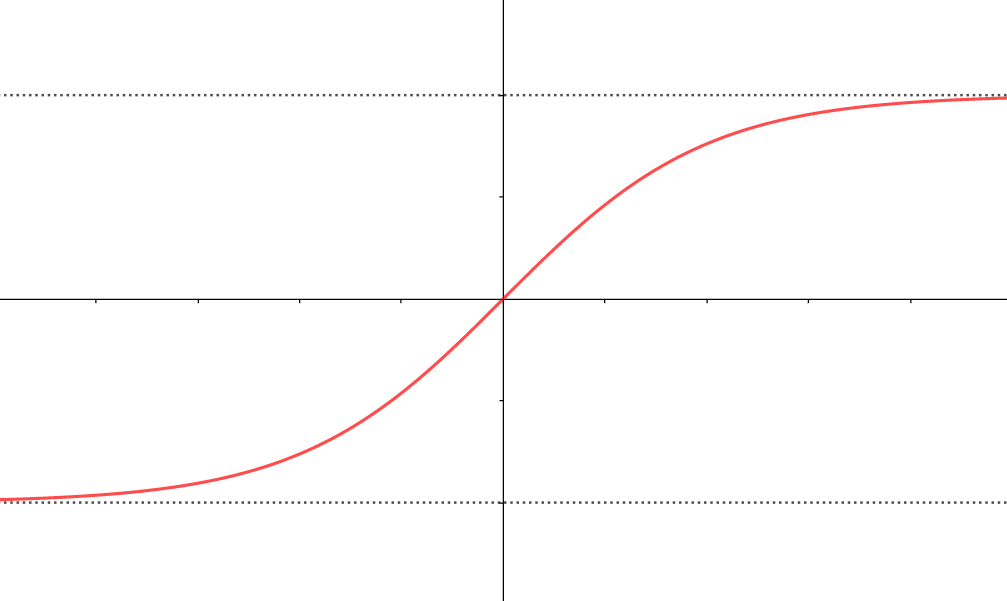
\includegraphics[scale = 0.4]{Tanh.PNG}
            \caption{Graphe de la fonction tangente hyperbolique}
            \end{figure}
            
            \begin{prop}\begin{leftbar}
                La loi de transformation des vitesses pour la rapidité est linéaire et 
                \begin{equation}
                    \varphi_{\R_1} = \varphi_{\R_2}+\varphi_{\nicefrac{\R_2}{\R_1}}.
                \end{equation}
            \end{leftbar}\end{prop}
            
            \begin{proof}
            ${}$\\
                En supposant que $\vv{v} = (v,0,0)$, on pose $v_{\R_1} ~\hat{=}~ \th{\varphi_{\R_1})},~ v_{\R_2} ~\hat{=}~ \th{\varphi_{\R_2}}$ et $v_{\nicefrac{2}{1}} ~\hat{=}~ \th{\varphi_{\nicefrac{\R_2}{\R_2}}}$, la loi de transformation \ref{LTVx} devient
                \begin{equation}
                    \th{\varphi_{\R_1}} = \frac{\th{\varphi_{\R_2}}+\th{\varphi_{\nicefrac{\R_2}{\R_1}}}}{1+\th{\varphi_{\R_2}}\th{\varphi_{\nicefrac{\R_2}{\R_1}}}} = \th{\varphi_{\R_2}+\varphi_{\nicefrac{\R_2}{\R_1}}}
                \end{equation}
                donc on trouve bien
                \begin{equation}
                    \varphi_{\R_1} = \varphi_{\R_2}+\varphi_{\nicefrac{\R_2}{\R_1}}.
                \end{equation}
            \end{proof}
            
            La dernière proposition montre bien que la condition $c\leq 1$ qui est souvent placée au centre la relativité einsteinienne n'est pas tellement fondamentale. Cette condition provient uniquement de notre paramétrisation de la vitesse.\\
            
            Une mauvaise interprétation de la condition $c\leq1$ (et donc $v\leq c$) peut aussi amener à croire que la distance maximale que l'on peut parcourir en un temps $\Delta t'$ est plus petite ou égale à $c\Delta t'$, ce qui est faux (cela dépend de l'objet qui se déplace). Un observateur peut se rendre n'importe où en n'importe quel temps. Par exemple, il est possible de se rendre à l'autre bout de la galaxie en une seconde et ceci n'est pas en contradiction avec $v\leq 1$. L'observateur qui se rend à l'autre bout de la galaxie ne se voit pas aller à une vitesse plus grande que $c$ par rapport aux éléments qu'il croise. Disons qu'il veut parcourir une distance $L$ vue par un observateur extérieur qui est dans le même référentiel que la galaxie, l'observateur qui se déplace dans la galaxie ne se voit pas parcourir une distance $L$ mais plutot une distance $L' = L\sqrt{1-v^2}\leq L$ où $v$ est la vitesse de son référentiel par rapport au référentiel de la galaxie. Donc il se voit aller à une vitesse
            \begin{equation}
                \frac{L'}{\Delta t'} = \frac{L}{\Delta t'} \sqrt{1-v^2} = \sqrt{1-v^2}.
            \end{equation}
            \comp
            Dans le référentiel de la galaxie, l'observateur qui se déplace n'est pas non plus vu comme allant à une vitesse supra-luminique à cause la dilatation du temps.\\
            
            On peut également définir l'impulsion.
            \begin{defn}
                On appelle \textit{quadri-impulsion} (ou \textit{énergie-impulsion}) le quadri-vecteur 
                \begin{equation}
                    P^\alpha = mU^\alpha
                \end{equation}
                où $m$ est la masse de l'objet considéré.
            \end{defn}
            En développant, on trouve que
            \begin{equation}
                P^\alpha = m U^\alpha = (\gamma m,\gamma m\vv{v}) = (E,\vv{p}).
            \end{equation}
            Ce quadri-vecteur est appelé énergie impulsion car sa partie spatiale correspond à l'impulsion classique multipliée par $\gamma$ (la partie spatiale correspond en fait à la quantité de mouvement mais on l'appelle souvent impulsion par anglicisme). La première composante est appelée \textit{énergie relativiste} et le second \textit{impulsion relativiste}.
            
            \begin{prop}\begin{leftbar}
                Nous avons l'égalité suivante.
                \begin{equation}
                    E^2 = \vv{p}^2 + m^2
                \end{equation}
            \end{leftbar}\end{prop}
            \begin{proof}
            ${}$\\
                Il suffit de développer l'expression de la norme de la quadri-impulsion.
                \begin{equation}
                P_\alpha P^\alpha = \vv{p}^2-E^2 = m^2\vv{v}^2\gamma^2-m^2\gamma^2 = -m^2
            \end{equation}
            \end{proof}
            
            Notons que la démonstration précédente implique bien que la masse (propre) est un invariant de Lorentz.\\
            
            Lorsque $\vv{p} = \vv{0}$, on retrouve l'équation bien connue
            \begin{equation}
                E = m.
            \end{equation}
            
            En mécanique classique, l'énergie et l'impulsion d'un système isolé sont conservées. Ceci est indépendant du principe de relativité. La relativité restreinte donne des nouvelles valeurs à l'énergie et à l'impulsion mais ces grandeurs restent conservées au sein d'un même référentiel.\\
            
            \begin{prin}[conservation de l'énergie impulsion]
            \begin{leftbar}
                Pour tout système isolé, l'énergie-impulsion est conservée au cours du temps.
            \end{leftbar}
            \end{prin}
            
        \subsection{Quadri-accélération}
        
            En dérivant à nouveau par rapport au temps propre $\tau$, on peut introduire un nouveau quadri-vecteur correspondant cette fois à l'accélération.
            \begin{defn}
                On appelle \textit{quadri-accélération} le quadri-vecteur
                \begin{equation}
                    A^\alpha ~\hat{=}~ \frac{d^2x^\alpha}{d\tau^2}.
                \end{equation}
            \end{defn}
            On peut montrer par un développement direct que, à $1+1$ dimensions,
            \begin{equation}
                A^\alpha = \frac{d^2x^\alpha}{d\tau^2} = \frac{dU^\alpha}{d\tau} = \gamma\frac{dU^\alpha}{dt} = \left( \frac{v}{(1-v^2)^{\frac{5}{2}}}\frac{dv}{dt}, \frac{v^2}{(1-v^2)^{\frac{5}{2}}}\frac{dv}{dt} +\gamma \frac{dv}{dt}\right)
            \end{equation}
        
            Tout en considérant des référentiels inertiels, rien n'empêche de considérer des objets qui accélèrent dans ces référentiels. Pour simplifier les calculs qui suivent, on considère le cas où les mouvements se font uniquement selon $x$. Le mouvement uniformément accéléré est défini en relativité einsteinienne comme la ligne d'univers telle qu'un observateur qui la suivrait ressente une accélération constante.
            
            \begin{defn}
                On appelle \textit{accélération propre}, l'accélération dans le référentiel tangent à la ligne d'univers d'un mouvement uniformément accéléré, c'est-à-dire le référentiel dans lequel l'observateur est immobile à l'instant considéré. C'est l'accélération ressentie par l'observateur.
            \end{defn}
            
            Supposons que l'observateur en MRUA suivent la trajectoire $(t(\tau),x(\tau))$ où $\tau$ est le temps propre, vu d'un référentiel $\mathcal{R}$ fixe de coordonnées $(t,x)$. A chaque instant $\tau$, on a un référentiel $\mathcal{R}_{\tau}$ obtenu par un boost de vitesse
            \begin{equation}
                v(\tau) = v_{\nicefrac{\R_\tau}{\R}}(\tau) = \frac{dx}{d\tau}.
            \end{equation}
            
            \begin{prop}\begin{leftbar}\label{prop:v}
                La vitesse de boost du référentiel fixe $\R$ au référentiel tangent $\R_\tau$ doit satisfaire
                \begin{equation}
                    \frac{dv}{d\tau} = a\left(1-v^2(\tau)\right).
                \end{equation}
            \end{leftbar}\end{prop}
            
            \begin{proof}
            ${}$\\
                Pour que le référentiel $\R_\tau$ soit tangent à tout instant $\tau$, $v(\tau)$ doit satisfaire
            \begin{equation}
                v(\tau+d\tau) = \frac{v(\tau)+ad\tau}{1+av(\tau)d\tau}
            \end{equation}
            Or, pour $\varepsilon\ll 1$,
            \begin{equation}
                \frac{1}{1+\varepsilon} = 1-\varepsilon+\dots
            \end{equation}
            et comme $d\tau$ est infinitésimale,
            \begin{align}
                \frac{v(\tau)+ad\tau}{1+av(\tau)d\tau} &\approx \left(v(\tau)+ad\tau\right)\left( 1-av(\tau)d\tau \right) \\
                &\approx v(\tau) + a\left( 1-v^2(\tau) \right)d\tau
            \end{align}
            On trouve donc bien que 
            \begin{equation}
                \frac{v(\tau+d\tau)-v(\tau)}{d\tau} = a\left( 1-v^2(\tau) \right).
            \end{equation}
            \end{proof}
            
            \begin{prop}\begin{leftbar}
                L'accélération propre est le taux de variation de la rapidité.
                \begin{equation}
                    a = \frac{d\varphi}{d\tau}
                \end{equation}
                De plus,
                \begin{equation}
                    v(\tau) = \th{a\tau}.
                \end{equation}
            \end{leftbar}\end{prop}
            
            \begin{proof}
            ${}$\\
                Il suffit de prendre $v(\tau) = \th{\varphi}$ auquel cas
                \begin{equation}
                    \frac{dv}{d\tau} = \left(1-\text{th}^2(\varphi)\right)\frac{d\varphi}{d\tau}.
                \end{equation}
                En comparant cette expression à celle de la proposition \ref{prop:v} on trouve bien 
                \begin{equation}
                    a = \frac{d\varphi}{d\tau}.
                \end{equation}
                Ceci implique que 
                \begin{equation}
                    \varphi(\tau) = a\tau+\varphi_0
                \end{equation}
                pour une certain constante d'intégration $\varphi_0$ qui peut être fixée à 0 sans perte de généralité. Par définition de $\varphi$ on trouve directement
                \begin{equation}
                    v(\tau) = \th{a\tau}.
                \end{equation}
            \end{proof}
            
            \begin{prop}\begin{leftbar}\label{eq:a}
                Le trajectoire d'un observateur en MRUA s'écrit explicitement en fonction du temps propre comme
                \begin{subequations}
                \begin{empheq}[left=\empheqlbrace]{align}
                    t(\tau) &= \frac{1}{a}\sh{a\tau}+t_0 \\
                    x(\tau) &= \frac{1}{a}\ch{a\tau}+x_0
                \end{empheq}
                \end{subequations}
            \end{leftbar}\end{prop}
            
            \begin{proof}
            ${}$\\
                On a 
                \begin{equation}
                    d\tau^2 = (1-v^2)dt^2 = \left( 1-\text{th}^2(\varphi) \right)dt^2 = \frac{dt^2}{\text{ch}^2{\varphi}}
                \end{equation}
                donc,
                \begin{equation}\label{eq:1}
                    \frac{dt}{d\tau} = \ch{\varphi}
                \end{equation}
                et
                \begin{equation}\label{eq:2}
                    \frac{dx}{dt} = v = \sh{\varphi}.
                \end{equation}
                En intégrant \ref{eq:1} et \ref{eq:2} on trouve bien le résultat voulu.
            \end{proof}
            
            On vient donc de voir que, quel que soit la nature de l'objet qui est en MRUA, sa trajectoire dans l'espace-temps a toujours la forme de celle explicité dans la proposition \ref{eq:a}, c'est-à-dire une hyperbole. Ces équations sont à comparer avec les équations du mouvement non-relativistes :
            \begin{subequations}\label{eq:hyperbole}
            \begin{empheq}[left=\empheqlbrace]{align}
                t(\tau) &= \tau\\
                x(\tau) &= at^2 + x_0
            \end{empheq}
            \end{subequations}
            pour lesquelles l'observateur n'a pas forcément une vitesse bornée.
            
            \begin{figure}[H]
            \centering
            \begin{tikzpicture}[scale = 1.2]
                \draw[->] (-4, 0) -- (4, 0) node[below right]{$x$};
                \draw[->] (0, -3) -- (0, 4) node[above left]{$t$};
                \draw[dotted, opacity = 0.9] (-3,-3) -- (3, 3);
                \draw[dotted, opacity = 0.9] (-3,3) -- (3, -3);
                \draw[domain = -3:3, smooth, blue] plot({sqrt(1 + \x*\x)}, \x);
                \draw[domain = -1.7:1.7, smooth,dashed] plot(\x*\x, \x);
            \end{tikzpicture}
            \caption{Trajectoire d'un objet en MRUA}
            \label{fig:my_label}
            \end{figure}
            
            Les formules précédentes prennent une forme simple dans le référentiel tangent à la ligne d'univers.\\
            
            Par définition, la norme d'un quadrivecteur est toujours un invariant de Lorentz. Les transformation de Lorentz sont des rotations hyperboliques et donc elles préservent les normes (isométries). La quantité $\underline{A}^2$ est un invariant de Lorentz. Or, dans le référentiel tangent à la ligne d'univers, $\underline{A}^2 = a^2$ où pour rappel $a$ est l'accélération propre. Donc dans n'importe quel référentiel on a
            \begin{equation}
                \underline{A}^2 = a^2.
            \end{equation}
        
        \subsection{Diagrammes d'espace-temps de Minkowski}
        
            Travaillons à une seule dimension d'espace pour simplifier les choses. Soient $\u{e_0} = (1,0)$ le vecteur temps unité (vecteur de type temps) et $\u{e_1} = (0,1)$ le vecteur espace unité (vecteur de type espace) dans un référentiel $\R$. Nous avons
            \begin{align}
                \u{e_0}^2 &= -1 \\
                \u{e_1}^2 &= 1
            \end{align}
            A quoi ressemble le vecteur temps unité dans un autre référentiel $\R'$ allant à la vitesse $v$ par rapport à $\R$ ? Pour cela, on fait un boost de Lorentz de paramètre $v$.
            \begin{equation}
                \begin{bmatrix}
                    \gamma & v\gamma \\
                    v\gamma & \gamma 
                \end{bmatrix}
                \begin{bmatrix}
                    1\\
                    0
                \end{bmatrix}=
                \begin{bmatrix}
                    \gamma\\
                    \gamma v
                \end{bmatrix}
            \end{equation}
            Les composantes du vecteur temps unité après le boost sont donc
            \begin{subequations}\label{eq:hyperbole}
            \begin{empheq}[left=\empheqlbrace]{align}
                x &= \frac{1}{\sqrt{1-v^2}}\\
                y &= \frac{v}{\sqrt{1-v^2}}
            \end{empheq}
            \end{subequations}
            On voit donc que $x$ et $y$ satisfont à la relation suivante.
            \begin{equation}
                x^2-y^2 = \frac{1}{1-v^2} - \frac{v^2}{1-v^2} = \frac{1-v^2}{1-v^2} = 1
            \end{equation}
            Donc, l'ensemble 
            \begin{equation}
            \left\{ \begin{bmatrix}
                \gamma & \gamma v \\
                \gamma v & \gamma 
            \end{bmatrix}
            \begin{bmatrix}
                    1\\
                    0
            \end{bmatrix} \Bigg\vert~ v\in\mathbb{R}\right\}
            \end{equation}
            
            est une hyperbole, ou plus exactement, la partie supérieure d'une hyperbole. Cette courbe est paramétrisée par la vitesse $v$. La partie inférieure de l'hyperbole apparaîtrais si l'on considérait les transformations de Lorentz non-orthochrones (nous avons juste considéré les transformations spéciales de Lorentz qui sont des transformations de Lorentz propres orthochrones).\\
            
            On peut faire le même raisonnement et trouver que 
            \begin{equation}
            \left\{ \begin{bmatrix}
                \gamma & \gamma v \\
                \gamma v & \gamma 
            \end{bmatrix}
            \begin{bmatrix}
                    0\\
                    1
            \end{bmatrix} \Bigg\vert~ v\in\mathbb{R}\right\}
            \end{equation}
            est également une hyperbole.
            
            \begin{figure}[H]
            \centering
            \begin{tikzpicture}[scale = 1.2]
                \draw[->] (-4, 0) -- (4, 0) node[below right]{$x$};
                \draw[->] (0, -3) -- (0, 4) node[above left]{$t$};
                \draw[dotted, opacity = 0.9] (-3,-3) -- (3, 3);
                \draw[dotted, opacity = 0.9] (-3,3) -- (3, -3);
                \draw[->, green] (-1.184, -3) -- (1.579, 4) node[right]{$t'$};
                \draw[->, green] (-4, -1.325)
                -- (4, 1.325) node[right]{$x'$};
                \draw[domain = -3:3, smooth, dashed] plot(\x, {sqrt(1 + \x*\x)});
                \draw[domain = -3:3, smooth, dashed] plot({sqrt(1 + \x*\x)},\x);
                \draw[very thick, <->] (0,1) node[below left]{$\u{e_0}$} -- (0,0) -- (1 , 0) node[below]{$\u{e_1}$};
                \draw[green, very thick, <->] (0.43,1.09) node[above left]{$\u{e_0}'$} -- (0,0) -- (1.06 , 0.35) node[above]{$\u{e_1}'$};
            \end{tikzpicture}
            \caption{Hyperbole unité de temps et hyperbole unité d'espace}
            \label{fig:my_label}
            \end{figure}
            
            La géométrie de l'espace-temps de Minkowski est dite \textit{hyperbolique}. Cela vient de la pseudo-métrique qui est elle-même hyperbolique. C'est pour cela qu'on appelle les transformations de Lorentz des \textit{rotations hyperboliques} et qu'elle prennent une forme particulièrement simple sous forme de cosinus et de sinus hyperboliques. Ceci explique aussi pourquoi la loi de composition des vitesses prend une forme extrêmement simple lorsqu'on l'exprime en terme de la rapidité.\\
            
            Notons que si l'on fixe $\u{e_0}' = (a,b)$ dans un boost à vitesse $v$, alors $\u{e_1}' = (c,d)$ est fixé par les relations
            \begin{align}
                \u{e_0}'^2 &= b^2-a^2 = -1 \\
                \u{e_1}'^2 &= c^2-d^2 = 1 \\
                \u{e_0}'\cdot\u{e_1}' &= bd-ac = 0
            \end{align}
            
            Les diagrammes de Minkowski sont plus simples lorsqu'on considère les T.S.L. comme des rotation hyperboliques. 
            \begin{prop}\begin{leftbar}
                Les T.S.L. prennent la forme suivante lorsqu'on les expriment sous forme d'une rotation hyperbolique
                \begin{subequations}\label{TSLh}
                \begin{empheq}[left=\empheqlbrace]{align}
                    t' &= t\ch{\varphi}-x\sh{\varphi} \\
                    x' &= x\ch{\vp}-t\sh{\vp} \\
                    y' &= y \\
                    z' &= z
                \end{empheq}
                \end{subequations}
            \end{leftbar}\end{prop}
            
            \begin{proof}
                Pour les mettre sous cette forme nous utilisons la rapidité. On sait que $v = \th{\varphi}$ ce qui entraîne que
                \begin{equation}
                    \gamma = \frac{1}{\sqrt{1-\text{th}^2(\varphi)}} = \ch{\varphi}
                \end{equation}
                et donc
                \begin{equation}
                    v\gamma = \th{\varphi}\ch{\varphi} = \sh{\varphi}.
                \end{equation}
            \end{proof}
            \comp
            
            
            \subsubsection{Dilatation des temps}
            \comp
            
                Soient un évènement $A$ de coordonnées $(t_A,0)$ et $(t_A',0)$ alors
                \begin{equation}
                    t_A' = \gamma t_A \geq t_A
                \end{equation}
            
                \begin{figure}[H]
                \centering
                \begin{tikzpicture}[scale = 1.2]
                    \draw[->] (-4, 0) -- (4, 0) node[below right]{$x$};
                    \draw[->] (0, -3) -- (0, 4) node[above left]{$t$};
                    \draw[dotted, opacity = 0.9] (-3,-3) -- (3, 3);
                    \draw[dotted, opacity = 0.9] (-3,3) -- (3, -3);
                    \draw[->, green] (-1.184, -3) -- (1.579, 4) node[right]{$t'$};
                    \draw[->, green] (-4, -1.325) -- (4, 1.325) node[right]{$x'$};
                    \draw[domain = -3:3, smooth, dashed] plot(\x,{sqrt(1 + \x*\x)});
                    \draw (0.36,1.06) node[scale = 0.6]{$\bullet$};
                \end{tikzpicture}
                \caption{Trajectoire d'un objet en MRUA}
                \label{fig:my_label}
                \end{figure}
            
            \subsubsection{Contraction des longueurs}
            
                \comp
            
        \subsection{Relativité et mécanique quantique}
            
            Dans cette partie nous discuterons de manière qualitative trois conséquences du mariage entre la relativité restreinte et la mécanique quantique. Le but n'est pas de présenter des raisonnements rigoureux mais plutôt de se faire une intuition derrière ces différents phénomènes.\\
            
            Soient un référentiel $\R$ de coordonnées $(t,x)$, un second référentiel $\R'$ de coordonnées $(t',x')$ en translation à vitesse $v$ par rapport à $\R$ et deux évènements $X_1 = (x_1^0,\vv{x}_1)$, $X_2 = (x_2^0,\vv{x}_2)$ tels que $x_1^0<x_2^0$. Prenons $X_1$ comme étant une désintégration d'une particule $A$ et deux particules $B$ et $C$ et $X_2$ comme étant une absorption d'une particule extérieure $D$ par $B$ pour former une particule $E$.
            \begin{equation}
                X_1 : A\to B+C \text{\quad puis \quad} X_2 : B+D\to E
            \end{equation}
            Comme ces évènement sont causalement reliés, l'intervalle d'espace-temps $(X_2-X_1)^2$ est de type temps (la particule $B$ ne peut pas aller plus vite que la vitesse de la lumière).
            \begin{equation}
                (X_2-X_1)^2 = (\vv{x}_2-\vv{x}_1)^2 - (x_2^0-x_1^0)^2 < 0
            \end{equation}
            Cependant, si l'on suppose que $(X_2-X_1)^2 > 0$, le principe d'incertitude d'Heisenberg donne une indétermination sur la vitesse de la particule $B$ qui permet de tout de même aller de $\vv{x}_1$ à $\vv{x_2}$. La probabilité que cela arrive est non-négligeable si
            \begin{equation}
                (\vv{x}_2-\vv{x}_1)^2 - (x_2^0-x_1^0)^2 \lesssim \frac{\hbar^2}{m^2}.
            \end{equation}
            On se retrouve donc avec deux évènements causalement reliés mais dont l'intervalle d'espace-temps est de type espace. C'est en contradiction avec ce que l'on a vu jusqu'à présent. Cela pose problème étant donné que comme l'intervalle est de type espace il est possible de trouver référentiel dans lequel $x_1'^0 > x_2'^0$. Qu'advient-il de la causalité dans ce cas-là ? Comment l'observateur pourrait-il voir la particule $B$ absorber une autre particule avant de voir la particule $B$ être créée?\\
            
            La seule solution à ce paradoxe est qu'il existe une autre particule $\overline{C}$ telle que l'observateur dans le référentiel $\R'$ observe
            \begin{equation}
                X_2 : D\to E+\overline{C} \text{\quad puis \quad} X_1 : \overline{C}+A\to B.
            \end{equation}
            Par conservation de la charge, il faut que $Q_{\overline{C}} = -Q_C$ et comme la masse est un invariant de Lorentz (norme de la quadri-impulsion) on trouve $m_{\overline{C}} = m_C$. $\overline{C}$ est l'anti-particule de $C$.\\
            
            Nous avons vu que le principe d'incertitude permet, dans une très petite région de l'espace, d'observer un déplacement d'une particule plus rapide que la lumière. Supposons donc maintenant que l'on voit une particule se déplacer plus vite que la lumière dans un référentiel $\R$. Cela veut dire que la ligne d'univers a, à un certain endroit, une pente plus grande que celle permise par le cône de lumière. Si l'on observe l'intersection des lignes de simultanéité d'un autre référentiel $\R'$ avec cette courbe, on voit que aux endroits où la particule est plus rapide que la lumière, il y a plusieurs intersection.
            
            \begin{figure}[H]
            \centering
            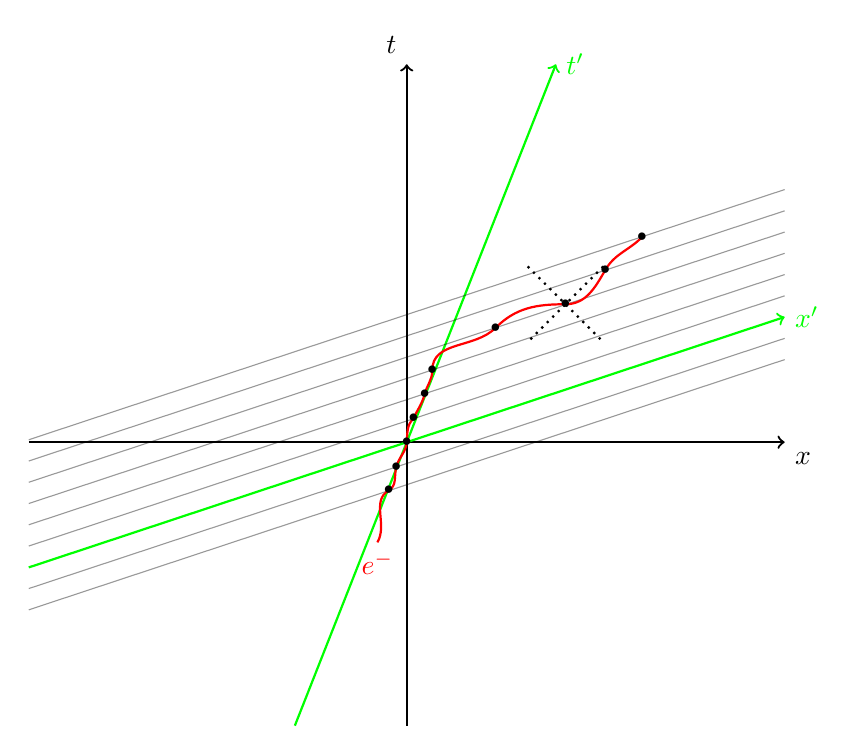
\begin{tikzpicture}[scale = 1.2]
                \draw[->, thick] (-4, 0) -- (4, 0) node[below right]{$x$};
                \draw[->, thick] (0, -3) -- (0, 4) node[above left]{$t$};
                %\draw[dotted, opacity = 0.9] (-3,-3) -- (3, 3);
                %\draw[dotted, opacity = 0.9] (-3,3) -- (3, -3);
                \draw[->, green, thick] (-1.184, -3) -- (1.579, 4) node[right]{$t'$};
                \draw[->, green, thick] (-4, -1.325) -- (4, 1.325) node[right]{$x'$};
                \draw[domain = -4:4, opacity = 0.4] plot(\x, {-0.225 + 0.331*\x});
                \draw[domain = -4:4, opacity = 0.4] plot(\x, {-0.45 + 0.331*\x});
                \draw[domain = -4:4, opacity = 0.4] plot(\x, {0.225 + 0.331*\x});
                \draw[domain = -4:4, opacity = 0.4] plot(\x, {0.45 + 0.331*\x});
                \draw[domain = -4:4, opacity = 0.4] plot(\x, {0.675 + 0.331*\x});
                \draw[domain = -4:4, opacity = 0.4] plot(\x, {0.9 + 0.331*\x});
                \draw[domain = -4:4, opacity = 0.4] plot(\x, {1.125 + 0.331*\x});
                \draw[domain = -4:4, opacity = 0.4] plot(\x, {1.35 + 0.331*\x});
                \draw[>=latex, red, thick] (-0.31, -1.06) node[below]{$e^-$} to[out = 60, in = 210] (-0.19, -0.51) node[black, scale = 0.7]{$\bullet$} to[out = 30, in = 255] (-0.11, -0.26) node[black, scale = 0.7]{$\bullet$} to[out = 75, in = 265] (0, 0) node[black, scale = 0.7]{$\bullet$} to[out = 85, in = 225] (0.07, 0.25) node[black, scale = 0.7]{$\bullet$} to[out = 65, in = 255] (0.19, 0.51) node[black, scale = 0.7]{$\bullet$} to[out = 75, in = 270] (0.27, 0.76) node[black, scale = 0.7]{$\bullet$} to[out = 90, in = 225] (0.94, 1.21) node[black, scale = 0.7]{$\bullet$} to[out = 45, in = 180] (1.68, 1.46) node[black, scale = 0.7]{$\bullet$} to[out = 0, in = 240] (2.1, 1.82) node[black, scale = 0.7]{$\bullet$} to[out = 60, in = 225] (2.49, 2.17) node[black, scale = 0.7]{$\bullet$};
                \draw[dotted,thick] (2.08,1.86) -- (1.28,1.06);
                \draw[dotted,thick] (1.28,1.86) -- (2.08,1.06);
            \end{tikzpicture}
            \label{fig:my_label}
            \caption{Ligne d'univers d'une particule supra-luminique}
            \end{figure}
            
            On peut alors faire un boost pour passer au référentiel $\R'$ afin de voir à quoi ressemble la ligne d'univers dans ce référentiel-là.
            
            \begin{figure}[H]
            \centering
            \begin{tikzpicture}[scale = 1.2]
                \draw[->, thick] (-4, 0) -- (4, 0) node[below right]{$x'$};
                \draw[->, thick] (0, -3) -- (0, 4) node[above left]{$t'$};
                \draw[domain = -4:4, opacity = 0.7] plot (\x, {0.35}) node[right]{$t'_1$};
                \draw[domain = -4:4, opacity = 0.7] plot (\x, {0.7});
                \draw[domain = -4:4, opacity = 0.7] plot (\x, {1.05});
                \draw[domain = -4:4, opacity = 0.7] plot (\x, {1.4});
                \draw[domain = -4:4, opacity = 0.7] plot (\x, {1.75}) node[right]{$t'_2$};
                \draw[>=latex, thick, red, ->] (-1, -2) node[below]{$e^-$} to[out = 70, in = 230] (0,0) ;
                \draw[>=latex, thick, red, ->] (0,0) to[out = 50, in = 180] (1.3, 1.75);  
                \draw[>=latex, thick, red, ->] (1.3, 1.75) to[out = 0, in = 180] (2.6, 0.35);
                \draw[>=latex, thick, red, ->] (2.6, 0.35) to[out = 0, in = 250] (3.9, 2.5);
            \end{tikzpicture}
            \label{fig:my_label}
            \caption{Ligne d'univers d'une particule supra-luminique}
            \end{figure}
            
            On voit bien que les lignes de simultanéité s'intersectionnent plusieurs fois avec la ligne d'univers ce qui veut dire qu'un observateur dans le référentiel $\R'$ voit plusieurs particules en même temps.\\
            
            La première chose importante est que l'on a supposé dès le départ que l'on était dans un cadre quantique. Ce genre de phénomène n'est pas observable dans un cadre purement relativiste. On voit que le nombre de particule n'est pas conservé. Si l'on voit une particule dans un certain référentiel, on peut en voir plusieurs dans un autre. Ceci suggère que le nombre de degré de liberté d'une théorie quantique relativiste devrait être infini. Les objets physiques qui ont cette caractéristiques sont les champs. On parle alors de théorie quantique des champs (QFT).\\
            
            La dernière conséquence du mariage de la relativité et de la mécanique quantique dont nous parlerons ici est le théorème spin-statistique. Ce théorème relie la nature du spin d'une particule d'une particule (spin entier ou demi-entier) à sa distribution statistique (Bose-Einstein ou Fermi-Dirac). Les détails mathématiques de cette correspondance dépasse cependant le cadre de ces notes.

\chapter{Théorie relativiste de la gravitation : fondements}

    \section{Principe d'équivalence}
    
        Quelle que soit la relativité (galiléenne ou einsteinienne), rien n'explique pourquoi les référentiels inertiels sont tels que observés. L'observation montre que le référentiel lié au soleil avec des axes pointants vers les étoiles "fixes" est un excellent référentiel inertiel. Cependant, si l'on prend du recul, ce référentiel n'est pas mieux qu'un autre. Qu'est-ce qui détermine les référentiels inertiels alors ?\\
            
        Voici une petite expérience de pensée qui permet de mieux se rendre compte du problème. Imaginons être dans le vide, sans lumière, sans son, sans aucun repère. Juste en face de nous, flottent deux boules de liquide, du whisky par exemple. Celle de gauche est sphérique et celle de droite est ellipsoïdale. On peut alors dire que la boule de gauche est immobile dans un référentiel $\R$ et que celle de droite est en rotation par rapport à $\R$. Mais qu'est-ce qui détermine ce référentiel à ce point dans l'espace ?\\
        
        Le physicien E. Mach avait déjà mis en évidence la relation entre les référentiels inertiels et les étoiles "fixes", c'est-à-dire la distribution de masse dans l'univers. Il a alors tenté d'appliquer ce principe en mesurant une potentielle différence de force d'inertie entre le plan de la galaxie et le plan transverse. Mais en réalité, il n'existe pas d'anisotropie de l'inertie, cependant l'idée de Mach est conceptuellement correcte.\\
        
        Ce problème est en fait lié au premier problème dont nous avons déjà parlé : mettre en place en théorie relativiste de la gravitation.
    
        \subsection{Énoncé du principe}
        
            Commençons par discuter le principe d'équivalence dans sa version la plus traditionnelle.
            
            \begin{prin}[d'équivalence, première formulation]
            \begin{leftbar}
                La masse gravitationnelle est égale à la masse inertielle.
            \end{leftbar}
            \end{prin}
            
            Dans sa seconde loi, Newton nous dit que pour un corps de masse $m_i$, la force résultante qui s'exerce sur ce corps est reliée à son accélération par
            \begin{equation}
                \vv{F} = m_i\vv{a}.
            \end{equation}
            
            D'un autre coté, la loi de la gravitation universelle de Newton dit que le champ de gravitation créé par un corps de masse $m_g$ situé en $O$ est donné par
            \begin{equation}
                \vv{g}(M) = -\frac{m_g G}{\abs{\vv{OM}}^3}\vv{OM}.
            \end{equation}
            
            Mais rien ne garanti que les paramètres $m_i$ et $m_g$ soient identiques. A priori, ce sont deux propriétés distinctes d'un corps qui apparaissent dans deux phénomènes différents. La masse apparaissant dans la seconde loi de Newton est appellée \textit{masse inertielle} et la masse apparaissant dans la loi de la gravitation universelle est appelée \textit{masse gravitationnelle} (c'est la "charge gravitationnelle").\\
            
            Si $m_i\neq m_g$, il y aurait des conséquences mesurables. Prenons l'exemple d'un pendule : dans un régime de petites oscillations, la période est donnée par
            \begin{equation}
                T = 2\pi\sqrt{\frac{m_iL}{m_g g}}
            \end{equation}
            où $L$ est la longueur du pendule. L'expérience d'Eötvos permet également de calculer le rapport $\nicefrac{m_i}{m_g}$ avec une très grande précision. Celle-ci fonctionne comme suit : on suspend deux corps différents à chaque extrémité d'une barre qui est elle-même suspendue à un support fixe. Alors, si les corps ont des masses de rapport $\nicefrac{m_{i}}{m_g}$ différents, les forces d'inerties dûes à la rotation de la Terre devraient entraîner une torsion sur le fil. Cette expérience a pu montrer que $m_i = m_g$ avec une très grande précision.\\
            
            En 1907, Einstein va prendre cette idée très au sérieux et partir de cette hypothèse pour construire une théorie relativiste de la gravitation qui sera aussi automatiquement une théorie de l'inertie.\\
            
            Observons une conséquence de cette hypothèse. Supposons que l'on ait le bilan de forces suivant dans un référentiel inertiel $\R_1$:
            \begin{equation}
                m_i\vv{a}_{\R_1} = m_g\vv{g} + \vv{F}.
            \end{equation}
            Dans un référentiel $\R'$, il y a des forces d'entraînement et des forces d'inertie qui apparaissent:
            \begin{equation}
                m_i\vv{a}_{\R_2} = m_g\vv{g} -m_i\vv{a}_e-m_i\vv{a}_i + \vv{F}.
            \end{equation}
            En regroupant les termes et en utilisant le principe d'équivalence, nous pouvons interpréter le référentiel $\R_2$ comme étant lui-même inertiel mais dont le champ de gravitation est maintenant $\vv{g}'$.
            \begin{equation}
                m\vv{a}_{\R_2} = m(\underbrace{\vv{g} -\vv{a}_e-\vv{a}_i}_{\vv{g}'}) + \vv{F}
            \end{equation}
            Il n'est donc pas possible, si $m_i=m_g$, de distinguer les effets d'une force gravitationnelle et d'une force d'inertie : c'est le principe d'équivalence entre gravitation et inertie. Passons maintenant à une formulation plus précise du principe d'équivalence.
            
            \begin{prin}[d'équivalence, deuxième formulation]
            \begin{leftbar}
                Dans une région suffisamment petite de l'espace-temps, il est toujours possible de choisir un référentiel dans lequel le champ de gravitation s'annule.
            \end{leftbar}
            \end{prin}
        
            Cette formulation du principe est beaucoup plus géométrique, on verra dans la suite que l'on peut considérer l'espace-temps comme un espace courbe. Le principe d'équivalence stipule qu'il est toujours possible de trouver un système de coordonnées tel que l'espace-temps est localement assimilable à un plan, c'est-à-dire à l'espace-temps plat de Minkowski. Cette idée permettra de relier le champ de gravitation aux propriétés géométriques de l'espace-temps.
        
        \subsection{Applications simples du principe d'équivalence}
        
            \subsubsection{Déviation d'un rayon lumineux par un champ de gravitation}
            
                Si un objet peut être vu comme allant en ligne droite dans un référentiel, un changement de référentiel (rotation) permet de le voir se déplacer suivant une trajectoire courbe. En utilisant le principe d'équivalence, ceci implique que le champ de gravitation peut dévier les rayons lumineux.\\
                
                Imaginons une étoile située derrière le soleil du point de vue de la Terre. On peut montrer en mécanique classique que n'importe quel corps allant à une vitesse $\vv{v} = \vv{c}$ subirait un angle de déviation
                \begin{equation}
                    \Delta\varphi = 2\frac{GM_\odot}{ac^2}
                \end{equation}
                où $a$ est le paramètre d'impact. Cette formule peut être obtenue en quasi-totalité par analyse dimensionnelle mais le facteur 2 lui provient des lois de Newton. En voyant la lumière comme composée de corps massiques on obtient alors que les rayons lumineux provenant d'une étoile derrière le soleil seraient déviés d'un angle $\Delta\varphi$.\\
                
                Les mêmes calculs dans la théorie d'Einstein permettent de trouver un angle de déviation
                \begin{equation}
                    \Delta\varphi = 4\frac{GM_\odot}{ac^2}
                \end{equation}
                au premier ordre. Le facteur $4$ est bien différent de celui prédit par Newton.\\
                
                En 1919, A. Eddington a organisé une expédition lors d'une éclipse solaire totale pour mesurer l'angle de déviation des rayons parvenant d'une étoile par le soleil. Les résultats sont précisément ceux prédit par le théorie d'Einstein. C'est une des premières validations expérimentales de la relativité générale.
            
                \begin{figure}[H]
                \centering
                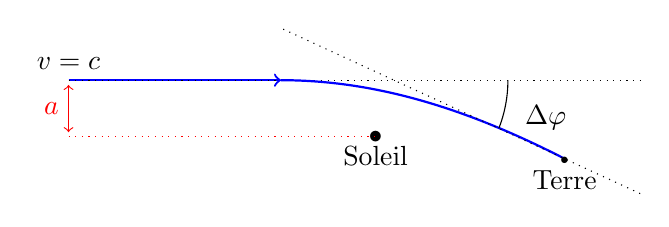
\begin{tikzpicture}[scale = 6]
                    \draw[->, thick, blue] (-0.45, 0) node[above, black]{$\Vec{v} = \Vec{c}$} -- (0,0);
                    \draw[dotted] (-0.45, 0) -- (0.76,0);
                    \draw[domain = 0:0.6, thick, smooth, blue] plot(\x, {-sqrt(1 + \x*\x) + 1});
                    \draw (0.48, 0) arc (0: -21.3 : 0.28);
                    \draw[dotted] (0.76, -0.24) -- (0,0.11);
                    \draw (0.56, -0.08) node{$\Delta \varphi$};
                    \draw (0.6, -0.17) node[scale = 0.6]{$\bullet$} node[below]{Terre};
                    \draw (0.2, -0.12) node{$\bullet$} node[below]{Soleil};
                    \draw[<->, red] (-0.45, -0.01) -- (-0.45, -0.11) node[midway, left]{$a$};
                    \draw[dotted, red] (-0.45, -0.12) -- (0.2, -0.12);
                    \end{tikzpicture}
                \label{fig:my_label}
                \caption{Déviation d'un rayon lumineux par le soleil}
                \end{figure}
            
            \subsubsection{Distorsion du temps par un champ de gravitation}
            
                On regarde les phénomènes sur une échelle de distance $h$. Quelle est la variation typique d'un potentiel gravitationnel sur échelle $h$ ? Considérons deux observateurs $A$ et $B$ au voisinage d'un astre de masse $M$ tels que $z_B-z_A\equiv h>0$ où $z$ dénote l'altitude. Le potentiel newtonnien généré par l'astre est
                \begin{equation}
                    V(z) = \frac{GM}{z}
                \end{equation}
                Ainsi, la différence de potentiel entre observée entre les points $A$ et $B$ est
                \begin{equation}
                    V(z_B)-V(z_A) = GM\left( \frac{1}{z_A+h} -\frac{1}{z_A}\right)=-\frac{GM}{z^2_A}h+\order{H^2} = g(z_A)h +\order{h^2}
                \end{equation}
                où $g$ est e champ de gravitation local. Nous obtenons $\delta V\sim gh$.
                \begin{defn}
                    On définit le \textit{paramètre de relativité} comme le rapport
                    \begin{equation}
                        \Xi = \frac{\abs{V}}{c^2}.
                    \end{equation}
                    où $\abs{V}$ est l'échelle de potentiel considérée.
                \end{defn}
                \begin{defn}
                La \textit{limite de champ faible} exprime le fait que l'approximation newtonienne et bonne, c'est-à-dire que
                \begin{align}
                    \Xi\ll1.
                \end{align}
                \end{defn}
                Dans notre cas, $\frac{gh}{c^2}\ll1$.\\
            
                On considère un champ de gravitation constant $\vv{g}=-g\vv{u}_z$ dans le référentiel $\R$ et deux observateurs : $E$ (émetteur) situé à un hauteur $z_E$ et $R$ (récepteur) situé à une hauteur $z_R = z_E+h$. Supposons que l'émetteur émette un signal, de période $(\delta t)_E = t_2^E-t_1^E$. Le signal est reçu par un le récepteur aux temps $t_1^R,t_2^R$, il observe donc une période $(\delta t)_R = t_2^R-t_1^R$. En vertu du principe d'équivalence, ce champ de gravitation est équivalent à un observateur uniformément accéléré dans la direction $\vv{u}_z$. De ce point de vue, $E$ et $R$ ont les positions
                \begin{align}
                    z_E(t) &=  \frac{1}{2}gt^2 \\
                    z_R(t) &= h  \frac{1}{2}gt^2
                \end{align}
                Si $z_1(t)$ et $z_2(t)$ sont les trajectoires des pulses alors
                \begin{align}
                    z_1(t) &= c(t-t^E_1) \\
                    z_2(t) &= c(t-t_2^E)
                \end{align}
                
                % schéma Eliott
                
                Calculons les temps de réception. Par définition, on doit avoir
                \begin{subequations}
                \begin{empheq}[left=\empheqlbrace]{align}
                    z_1(t_1^R-t^E_1) &= z_R(t_1^R) \\
                    z_2(t_2^R) &= z_R(t_2^R)
                \end{empheq}
                \end{subequations}
                autrement dit,
                \begin{subequations}
                \begin{empheq}[left=\empheqlbrace]{align}
                    ct_1^R &= h-\frac{1}{2}g(t_1^R)^2 \\
                    c(t_2^R-t_2^E) &= h-\frac{1}{2}g(t_2^R)^2
                \end{empheq}
                \end{subequations}
                Si l'on considère le cas $\dot{z}_1(t),\dot{z}_2(t)\ll c$ et $gt\ll c$ (limite de champ faible), on peut alors développer au premier ordre après avoir soustrait les deux équations précédentes.
                \begin{equation}
                    c\left( (\delta t)_R-(\delta t)_E \right) = \frac{1}{2}g\left( (t_2^R)^2-(t_1^R)^2 \right) \approx \frac{gh}{c}(\delta t)_R
                \end{equation}
                On trouve alors que
                \begin{align}
                    (\delta t)_R-(\delta t)_E &=  \frac{gh}{c^2}(\delta t)_R \\
                    \Leftrightarrow\quad (\delta t)_E &= \left( 1-\frac{gh}{c^2} \right)(\delta t)_R  \\
                    \Leftrightarrow\quad \nu_R &= \left( 1-\frac{gh}{c^2} \right)\nu_E
                \end{align}
                où $\nu_E = \frac{1}{(\delta t)_E}$, $\nu_R = \frac{1}{(\delta t)_R}$ sont respectivement les fréquences d'émission et de réception.\\
                
                En posant $\nu\approx \nu_1 \approx \nu_2$ (la différence entre $\nu_1$ et $\nu_2$ est très petite),
                \begin{equation}
                    \frac{\Delta\nu}{\nu} = -\frac{gh}{c^2}
                \end{equation}
                
                Voici un second raisonnement : lorsque l'observateur accéléré arrive au niveau de $R$, il coïncide avec un observateur de vitesse constante $v = g(\delta t)_E = \frac{gh}{c}$. Par effet Doppler, ce dernier observe une plus petite fréquence que celle à laquelle $E$ a émit le signal.
                \begin{equation}
                    \frac{\nu_E}{\nu_R} = \sqrt{\frac{1+\frac{gh}{c^2}}{1-\frac{gh}{c^2}}}\approx 1+\frac{gh}{c^2}.
                \end{equation}
                ce qui correspond au résultat que nous avions trouver en premier lieu. La fréquence observée est donc plus petite que le fréquence émise.\\
                Pour un champ non-uniforme, cette formule se généralise comme
                \begin{equation}
                    \frac{\Delta\nu}{\nu} = -\frac{\Delta\phi}{c^2}
                \end{equation}
                où $\varphi$ est le potentiel du champ $\vv{g}$, c'est-à-dire le champ tel que $\vv{g} = -\vv{\nabla}\varphi$.
                
                \begin{exmp}
                    Pour un rayon lumineux en provenance du soleil, $\varphi=-\frac{GM_\odot}{r}$ et donc
                    \begin{equation}
                        \Delta\varphi = -\frac{GM_\odot}{r_{\odot-\oplus}} + \frac{GM_\odot}{R_\odot}\approx\frac{GM_\odot}{R_\odot}.
                    \end{equation}
                    Ceci donne
                    \begin{equation}
                        \frac{\Delta\nu}{\nu} \approx - \frac{GM_\odot}{R_\odot c^2} = -\varepsilon_\odot \sim 10^{-6}.
                    \end{equation}
                    Il y a donc un décalage vers le rouge lorsque les rayons remontent le champ de gravitation. Cet effet est observable pour les raies spectrales.
                \end{exmp}
                
                On voit le temps des satellites en orbite autour de la Terre dilaté par effet cinématique (relativité restreinte) mais il y a aussi un effet inverse dû au champ de gravitation terrestre. On verra qu'il existe une orbite où ces effets se compensent.
    
        \subsection{Principe de covariance générale}
        
            Le principe d'équivalence dit que, localement dans l'espace-temps, les effets du champ de gravitation peuvent êtres annulé par un choix de référentiel approprié (référentiel localement inertiel). Pour connaître les lois de la physique en présence de gravitation dans un référentiel quelconque $\R$, il suffit donc faire un changement de référentiel à partir d'un référentiel localement inertiel (où les lois des la physique sont déjà connues mais sans gravitation) à $\R$. Donc, le principe d'équivalence permet de déduire les effets du champ de gravitation lorsque l'on connaît les lois de la physique en l'absence de gravitation, c'est un \textit{principe de covariance} et non un \textit{principe de symétrie} (ou \textit{principe d'invariance}).\\
            
            En particulier, ce principe est de nature fondamentalement différente du principe de relativité einsteinienne qui est un principe d'invariance. Ce dernier dit que les lois de la physique restent les mêmes (invariantes) sous les transformations du groupe de Poincaré. Ceci "contraint" la physique à s'écrire en terme de vecteurs (au sens de Poincaré), pas le principe d'équivalence.\\
            
            Néanmoins, les équations du champ de gravitation devront être décrites d'une manière générale dans tout les référentiels possibles, puisque l'effet des changements de référentiels n'est rien d'autre qu'un champ de gravitation. C'est le \textit{principe de covariance générale}. Il faut écrire les lois de la physique dans tout les référentiels. C'est une autre manière de reformuler le principe d'équivalence.
            
            \begin{prin}[de covariance générale]
            \begin{leftbar}
            Les lois de la physique doivent êtres écrites sous une forme qui ne fait référence à aucun référentiel.
            \end{leftbar}
            \end{prin}
            
            Le principe qui sous-tend la notion de covariance générale est qu'il n'existe a priori aucune coordonnée. Ces dernières sont seulement des artifices mathématiques utilisés pour décrire la nature et ne devraient donc jouer aucun rôle dans l'expression des lois de la physique. C'est une redondance et pas une symétrie, comme pour les transformations de jauge (ce qu'on appelle symétrie de jauge n'est en fait pas une symétrie).
    
    \section{Changement de référentiels et variétés}
    
        \subsection{Espaces courbes}
        
            En mécanique classique, la distance entre deux points est absolue. Ceci rend, entre autre, la notion de solide possible (ensemble de point à distance fixe). Mais en relativité restreinte ce n'est plus le cas. \\
            
            Notons $\M$ l'espace-temps. Quelle que soit sa nature, il doit être possible de "mettre" un système de coordonnées sur cet espace. L'espace-temps doit donc en quelque sorte être assimilable à $\mathbb{R}^4$. Rien ne dit qu'il doit exister une bijection de l'espace-temps de $\M$ dans $\mathbb{R}^4$ mais on doit en tout cas pouvoir couvrir $\M$ de domaines qui sont en bijection avec $\mathbb{R}^4$. C'est ici qu'intervient la notion de \textit{variété}.\\
            
            On commence par définir les fonctions qui font l'intermédiaire entre un ensemble quelconque (ici $\M$) et $\mathbb{R}^n$.
            \begin{defn}
                Une \textit{carte locale} $(U,\varphi)$ de dimension $n$ pour un ensemble $\M$ est une bijection
                \begin{equation}
                    \varphi:U\to\varphi(U) \subset\mathbb{R}^n
                \end{equation}
                où $U$ est un sous-ensemble de $\M$ appelé \textit{domaine de carte} et $\varphi(U)$ un ouvert de $\mathbb{R}^n$. La fonction $\varphi$ est appellée \textit{application de coordonnées}.
            \end{defn}
            
            Ce nom se justifie par le fait que notre fonction $\varphi$ est entièrement déterminée par ses coordonnées telles que $\varphi = (x^1, x^2, \ldots, x^n)$ où $x^i: U \to \mathbb{R}$ quel que soit $i$. Pour pouvoir couvrir tout l'espace-temps, nous avons besoin d'un ensemble de cartes dont les domaines recouvrent $\M$.
            
            \begin{defn}
                Un \textit{atlas différentiable} $\A$ de dimension $n$ pour un ensemble $\M$ est une collection 
                \begin{equation}
                    \A = \left\{ (U_i,\varphi_i)~|~i\in I \right\}
                \end{equation}
                de cartes locales de dimension $n$ pour $\M$ telle que
                \begin{enumerate}[label=\textit{(\roman*)}]
                    \item $\bigcup_{i\in I} U_i = \M$
                    \item si $U_i\cap U_j \neq \varnothing$ alors $\varphi_i(U_i\cap U_j)$ est un ouvert de $\Rm$ et les cartes $(U_i,\varphi_i)$ et $(U_j,\varphi_j)$ sont \textit{compatibles}, c'est-à-dire que l'application de changement de carte
                        \begin{equation}
                            \varphi_j\circ\varphi_i^{-1}:\varphi_i(U_i\cap U_j)\subset\Rm\to\varphi_j(U_i\cap U_j)\subset\Rm
                        \end{equation}
                        est différentiable (de classe $C^\infty$).
                \end{enumerate}
            \end{defn}
            
            Notons que nous travaillerons uniquement avec des applications différentiables. Pourquoi ne pas imposer directement que les applications de coordonnées soient différentiables ? A priori, $\M$ est juste un ensemble et ne comporte aucune structure supplémentaire, cette notion n'aurait donc pas de sens. De plus, nous verrons qu'un changement de carte correspond à un changement de référentiel. Les changements de carte doivent donc être différentiables afin de pouvoir écrire les lois de la physique (EDP) dans tous les référentiels. Ceci justifie l'utilisation de variétés dites "différentiables", et pas d'un autre type de variété.
            
            \begin{rmk}
                La condition de changement de carte différentiable permet en fait plus que cela. Lorsqu'on a une application entre deux variétés, on peut définir ce que différentiable signifie pour celle-ci. Pour que cette notion ne dépende pas des cartes choisies, il faut que les changement de carte soient eux aussi différentiables.
            \end{rmk}
            
            La prochaine définition demande de connaître plusieurs notions mathématiques que nous ne traiterons pas en détail dans ces notes.
            
            \begin{defn}
                Une \textit{variété différentiable} $(\M,\A)$ de dimension $n$ est un ensemble $\M$ munit d'un atlas différentiable de dimension $n$ tel que la topologie canonique associée soit séparée au sens de Hausdorff et à base dénombrable.
            \end{defn}
            
            Revenons sur les notions impliquées dans cette définition. Il possible de montrer qu'un ensemble de domaines de carte forme une topologie, on l'appelle \textit{topologie canonique}. On veut que cette topologie soit \textit{séparée au sens de Hausdorff}. Cela signifie que si l'on prend deux points $a, b \in \M$, il doit exister deux ouverts disjoints $U$ et $V$ tels que $a \in U$ et $b \in V$. Cela permet d'éviter le "dédoublement" de points. Pour finir, la topologie canonique doit aussi être \textit{à base dénombrable}, c'est-à-dire qu'il doit exister un ensemble dénombrable d'ouverts tels que n'importe quel autre ouvert peut s'exprimer comme une union (au plus dénombrable) d'ouverts de cet ensemble. Cette condition assure une certaine cohérence entre la dimension de la variété et l'ensemble en question. Sans cela, il serait, par exemple, possible de munir l'ensemble $\mathbb{R}^2$ d'un atlas de sorte à obtenir une variété différentiable de dimension $1$.
            
            \begin{rmk}
                Pour être rigoureux, on distingue la notion de structure différentiable et de variété différentiable. Une structure différentiable est une classe d'équivalence d'atlas différentiables. On dit que deux atlas sont équivalents si toutes leurs cartes sont compatibles, c'est-à-dire si l'union des deux atlas forme toujours un atlas différentiable. Notons que la donnée d'un atlas suffit à définir une classe d'équivalence. On définit alors une variété différentiable comme étant un ensemble munit d'une structure différentiable et dont la topologie canonique respecte les propriétés énoncées ci-dessus. Si l'on a une application $a$ entre deux variétés, on dit que $a$ est un homéomorphisme (notion d'équivalence pour les topologies) si $a$ est bijective et bicontinue. Les deux variétés sont alors homéomorphes. Si en plus $a$ est bidifférentiable, c'est un difféomorphisme et les variétés sont difféomorphes (notion d'équivalence pour les variétés différentiables). Si deux variétés sont difféomorphes elles sont aussi homéomorphes mais pas le contraire. Ceci permet au même ensemble d'avoir la même topologie canonique mais des structures différentiables non-difféomorphes. Par exemple il a été montré (Milnor, 1956) que la sphère $S^7$ munit de la topologie induite par la topologie usuelle de $\mathbb{R}^8$ possède 28 structures de variétés différentiables non-difféomorphes.
            \end{rmk}
            
            \begin{rmk}
                 Nous verrons dans l'on peut définir la notion de différentiabilité  pour une application entre deux variétés. On peut alors montrer que le fait d'imposer que les changements de carte soient différentiables implique que les carte sont aussi différentiables. Une variéte est donc localement difféomorphe à $\mathbb{R}^n$.
            \end{rmk}
            
            \begin{rmk}
                On définit une variété différentiable à bord de la même manière mais en remplaçant $\mathbb{R}^n$ par le demi-espace $\mathbb{R}^{n+}=\left\{(x_1,\dots,x_n)\in\mathbb{R}^n|x_1\geq 0\right\}$. Le bord, noté $\p\M$, est l'ensemble des points dont l'image par une application de coordonnée est sur le bord de $\mathbb{R}^{n+}$. Dans ce cas, $\p\M$ est une variété différentiable de dimension $n-1$ sans bord.
            \end{rmk}
            
            Si l'on suppose que l'espace-temps est une variété différentiable, quel que soit $P\in\M$ un évènement, on a alors un domaine de carte $U$ avec $P\in U$ et une application de coordonnées
            
            \begin{equation}\label{eq:coordloc}
            x:\left(
            \begin{array}{ccc}
                U & \longrightarrow & x(U) \subset \mathbb{R}^4  \\
                P & \longmapsto & x(P) = (x^0(P), x^1(P) , x^2(P), x^3(P))
            \end{array}
            \right).
            \end{equation}
            
            \begin{defn}
                Si $x$ est une carte locale en $P\in\M$, alors on appelle \textit{coordonnées locales} du point $P$ les applications $x^\mu$ telles que \ref{eq:coordloc}.
            \end{defn}
            
            On utilise la notation $(x^\mu(P)) \equiv (x^0(P),x^1(P),x^2(P),x^3(P))$. De manière générale, lorsque que le contexte est clair, on ne note pas la dépendance en le point de l'espace-temps. Par exemple, $g_{\mu\nu}(P)\equiv g_{\mu\nu}$. Gardons bien à l'esprit que les coordonnées locales $x^\mu$ sont des applications et que les $x^\mu(P)$ sont des nombres réels. 
            
            \begin{defn}
                On dit que le système de coordonnées $z$ est \textit{localement plat} en $P$ si $(z,U)$ est une carte locale telle que $P\in U$ et 
                \begin{subequations}\label{locin}
                \begin{empheq}[left=\empheqlbrace]{align}
                    g_{\mu\nu}(P) &= \eta_{\mu\nu}\\
                    \p_\alpha g_{\mu\nu}(P) &= 0
                \end{empheq}
                \end{subequations}
                On note l'application de coordonnée $z_P$.
            \end{defn}
            
            Si $z_P$ est un système de coordonnées localement plat en $P$, et $Q\in U$ alors $z_P^\alpha(Q)$ sont les coordonnées de $Q$ dans le système de coordonnées localement inertiel en $P$.\\
            
            Nous avons vu précédemment que référentiel et système de coordonnées sont des notions équivalentes. Un changement de référentiel n'est donc rien d'autre qu'un changement de carte. Soient deux applications de coordonnées (deux système de coordonnées) $x^\mu$ et $x'^\mu$ au point $P\in\M$, alors on peut alors exprimer les coordonnées $x'^\mu(P)$ en fonction des coordonnées $x^\mu(P)$.
            \begin{equation}\label{eq:chgtref}
                x'^\mu(P) = (x'\circ x^{-1})(x^\mu(P))
            \end{equation}
            
            \begin{defn}
                Une \textit{ligne d'univers} est une courbe différentiable dans la variété, c'est-à-dire une application
                \begin{equation}
                    \gamma : I\subset\mathbb{R} \to \M.
                \end{equation}
            \end{defn}
            On peut directement obtenir une courbe dans $\mathbb{R}^4$ à partir de celle dans $\mathcal{M}$.
            \begin{equation}
                x^\mu(\lambda)\equiv(x\circ\gamma)(\lambda)
            \end{equation}
            Nous voudrions exprimer cette courbe en fonction du temps propre mais cette notion n'est pas encore claire dans ce formalisme.\\
            
            Soit $P\in\M$ un évènement et $z^\alpha_P$ des coordonnées localement inertielles en $P$. L'existence d'un tel système de coordonnées est garantie par le principe d'équivalence. Par définition, le temps propre doit satisfaire
            \begin{equation}
                d\tau^2 = -\eta_{\alpha\beta}dz^\alpha_Pdz^\beta_P
            \end{equation}
            Dans un référentiel quelconque de coordonnées $x$, cette relation devient
            \begin{equation}\label{eq:met}
                d\tau^2 = -\eta_{\alpha\beta}\frac{\p z^\alpha_P}{\p x^\mu}\frac{\p z^\beta_P}{\p x^\nu}~dx^\mu dx^\nu
            \end{equation}
            où l'on a utilisé $\ref{eq:chgtref}$. On obtient une expression de $\eta_{\mu\nu}$ généralisée (aux référentiels non-localement inertiels). Même si cela peut paraître claire, nous définirons mieux les objets du type $dz^\alpha_P$ dans le suite, cela justifiera cette loi de transformation.
            
            \begin{defn}
                Si $z$ est un système de coordonnées localement inertiel en $P$ et $x$ un autre système de coordonnée en $P$, on définit le \textit{tenseur métrique} comme
                \begin{equation}
                    g_{\mu\nu}(P)~\hat{=}~\eta_{\alpha\beta}\frac{\p z^\alpha_P}{ \p x^\mu}\frac{\p z^\beta_P}{\p x^\nu}
                \end{equation}
            \end{defn}
            Notons bien que le tenseur métrique dépend du point de l'espace-temps en lequel il est considéré.\\
            La relation \ref{eq:met} devient
            \begin{equation}
                d\tau^2 = -g_{\mu\nu}~dx^\mu dx^\nu.
            \end{equation}
            
            \begin{prop}\begin{leftbar}
                Le tenseur métrique satisfait les propriétés suivantes.
                \begin{enumerate}[label = \textit{\roman*)}]
                    \item symétrie : $g_{\mu\nu}=g_{\nu\mu}$
                    \item métrique : $g_{\mu\nu}$ définit un produit scalaire qui a la même signature que $\eta$
                    \item si $g'_{\mu\nu}$ est le tenseur métrique dans les coordonnées $x'(x)$ alors
                    \begin{equation}
                        g'_{\mu\nu} = \frac{\p x^\rho}{\p x'^\mu}\frac{\p x^\kappa}{\p x'^\nu}~g_{\rho\kappa}.
                    \end{equation}
                \end{enumerate}
            \end{leftbar}\end{prop}
            
            \begin{proof}
                \begin{enumerate}[label = \textit{\roman*)}]
                    \item Direct en prenant la définition.
                    \item Les $\frac{\p z^\alpha_P}{\p x^\mu}$ sont les élément de matrice du jacobien de changement de coordonnée (matrice inversible), ce qui permet de conclure.
                    \item Soit $x'$ un autre système de coordonnées en $P$ et $g_{\mu\nu}'(P)$ le tenseur métrique dans ces coordonnées. En utilisant la chain rule nous trouvons que
                    \begin{align}
                        g_{\mu\nu}'(P) &= \eta_{\alpha\beta}\frac{\p z^\alpha_P}{ \p x'^\mu}\frac{\p z^\beta_P}{\p x'^\nu}\\
                        &= \eta_{\alpha\beta}\frac{\p x^\rho_P}{ \p x'^\mu}\frac{\p z^\alpha_P}{\p x^\rho}\frac{\p x^\kappa_P}{ \p x'^\nu}\frac{\p z^\beta_P}{d\p x^\kappa} \\
                        &= \frac{\p x^\rho_P}{ \p x'^\mu}\frac{\p x^\kappa_P}{ \p x'^\nu}g_{\rho\kappa}
                    \end{align}
                    Ceci est un exemple de transformation tensorielle, on généralisera cela dans la suite.
                \end{enumerate}
            \end{proof}
            
            \begin{prop}\begin{leftbar}
                Dans un référentiel localement inertiel, l'espace-temps est Minkowskien (espace-temps plat), c'est-à-dire que
                \begin{equation}
                    g_{\mu\nu}(P) = \eta_{\mu\nu}
                \end{equation}
            \end{leftbar}\end{prop}
            
            \begin{proof}
            ${}$\\
                Il suffit d'évaluer $g_{\mu\nu}$ dans le même référentiel inertiel de coordonnées inertielles $z^\alpha_P$.
                \begin{equation}
                    g_{\mu\nu}(P) = \eta_{\alpha\beta}\frac{\p z^\alpha_P}{ \p z^\mu}\frac{\p z^\beta_P}{\p z^\nu} =  \eta_{\alpha\beta}\delta_{\alpha\mu}\delta_{\beta\nu} = \eta_{\mu\nu}
                \end{equation}
            \end{proof}
            
            Malgré l'idée intuitive que l'on peut avoir de la notion de coordonnées localement inertielles, nous n'avons pas encore discuté la notion mathématique. Dans la démonstration de la proposition précédente nous n'avons pas exactement montré que le tenseur métrique prenait cette forme dans tout les référentiel localement inertiels, mais juste que s'il existe un tel référentiel alors le tenseur métrique est la pseudo-métrique Minkowskienne et donc en particulier diagonale. Mais cela provient en fait directement de la définition de $g_{\mu\nu}$ et de comment on a trouvé son expression dans un premier temps. Même si c'est bien de le vérifier, ce résultat n'est pas nouveau. On peut en fait se servir de la condition de diagonalité de la métrique pour définir mathématiquement ce que veut dire "localement inertiel". On ajoute une seconde condition qui donne l'idée de "plan tangent".
            
            \begin{prop}\begin{leftbar}
                On peut toujours trouver un système de coordonnée localement plat.
            \end{leftbar}\end{prop}
            
            \begin{proof}
            ${}$\\
                Le raisonnement suivant n'est pas une preuve rigoureuse mais plutot un exercice de comptage qui motive la proposition. Si l'on considère un espace-temps de dimension $D$, alors $g_{\mu\nu}$ possède $\frac{1}{2}D(D+1)$ composante indépendantes et $\p_\alpha g_{\mu\nu}$ possède $\frac{1}{2}D^2(D+1)$. Dans un changement de référentiel quelconque, on a $D^2$ paramètres correspondants aux éléments de matrice $\frac{\p x'(P)}{\p x}$ dans la loi de transformation de $g$. Pour la loi de transformation de $\p_\alpha g_{\mu\nu}$ on a $\frac{1}{2}D^2(D+1)$ paramètres associées aux éléments de matrice $\frac{\p^2 x'^\mu(P)}{\p x^\nu\p^\rho}$. En tout, nous avons donc
                \begin{equation}
                    \frac{1}{2}D(D+1)+\frac{1}{2}D^2(D+1)
                \end{equation}
                variables que l'on veut ajuster à l'aide de
                \begin{equation}
                    D^2+\frac{1}{2}D^2(D+1)
                \end{equation}
                paramètres. Ceci donne
                \begin{equation}
                    \#\text{paramètres}-\#\text{variables} = D^2-\frac{1}{2}D(D+1) = \frac{1}{2}D(D-1)\geq0.
                \end{equation}
                Ce qui suggère bien qu'il est toujours possible de choisir des coordonnées telles que \ref{locin}.
            \end{proof}
            
            Il existe une infinité des coordonnées localement inertielles en $P$, on se limite aux systèmes tels que $z^\alpha(P) = 0$. Ainsi, si l'on a deux systèmes de coordonnées localement inertielles $z^\alpha_P$ et $z'^\alpha_P$, 
            \begin{equation}
                z'^\alpha_P : \Lambda^\alpha_{~\beta}z^\beta_P+\mathcal{O}(z^3)
            \end{equation}
            avec $\Lambda\in SO(3,1)$.\\
            
            Peut-on également imposer que les dérivées secondes s'annulent ? Pour voir cela, faisons un comptage, de la même manière que dans la démonstration précédente. Le terme $\p_\mu\p_\nu g_{\rho\kappa}(P)$ possède $\left(\frac{1}{2}D(D+1)\right)^2$ composantes indépendantes et $\frac{\p^3 x^\mu}{\p x'^\nu\p x'^\rho\p x'^\kappa}$ possède
            \begin{equation}
                \left(\frac{1}{6}D(D-1)(D-2)+D(D-1)+D\right)D
            \end{equation} paramètres indépendants ($\#\text{ éléments avec 3 indices distincts }+~\#\text{ éléments avec 2 indices égaux }+\#\text{ éléments avec 3 indices égaux}$ multiplié par $D$ pour l'indice supérieur). Nous avons alors
            \begin{equation}
                \frac{1}{2}D(D+1)+\frac{1}{2}D^2(D+1)+\left(\frac{1}{2}D(D+1)\right)^2
            \end{equation}
            variables que l'on veut ajuster à l'aide de
            \begin{equation}
                D^2+\frac{1}{2}D^2(D+1)+\frac{1}{6}D^2(D-1)(D-2)+D^2(D-1)+D^2
            \end{equation}
            paramètres. Auquel cas,
            \begin{align}
                \#\text{paramètres}-\#\text{variables} &= \frac{D^2(D^2-1)}{10}+\frac{1}{2}D(D+1)-D^2\\
                &= \frac{1}{12}D(D-1)(D-2)(D+3)
            \end{align}
            Ce nombre est en fait lié a ce que l'on appelle un invariant de courbure.
            
            \begin{defn}
                En dimension $D$ le \textit{nombre d'invariants de courbure} est 
                \begin{align}
                    \mathscr{N}_D ~&\hat{=}~  \frac{D^2(D^2-1)}{12}+\frac{1}{2}D(D+1)-D^2\\
                &= \frac{1}{12}D(D-1)(D-2)(D+3)
                \end{align}
            \end{defn}
            Nous verrons dans la suite ce qu'est un invariant de courbure.\\
            Étudions le résultats pour quelques valeurs de $D$.
            \begin{itemize}[label = \textbullet]
                \item si $D=1$ : on a $g_{\mu\nu} = g$ un scalaire. La loi de transformation devient
                \begin{equation}
                    g' = \frac{\p x}{\p x'} g
                \end{equation}
                il est donc toujours possible de prendre $g=1$.
                \item si $D = 2$ : $\mathscr{N}_D = 0$ mais ce résultat n'est pas correcte car il y a un paramètre qui n'agit pas, ce dont nous n'avons pas tenu compte dans le raisonnement ci-dessus. En fait, $\mathscr{N}_D = 1$, ce qui rend impossible d'éliminer les dérivées secondes de la métrique, il y a donc une courbure.
                \item si $D=4$ (cas de l'espace-temps) : il y a $\mathscr{N}_D = 14$ invariants de courbure. Il y a un théorème de géométrie riemanienne qui dit que si ces 14 invariantes de courbures sont nulles, tout le reste est nul et il n'y a donc pas besoin de traiter les dérivées d'ordre plus élevé.
            \end{itemize}
            
            Peut-on avoir une intuition sur la manière de coder ces invariants de courbure ? Soit une quantité $t_{\mu_1\dots\mu_p}$ qui se transforme sous un changement de référentiel quelconque comme
            \begin{equation}
                t'_{\mu_1\dots\mu_p} = \frac{\p x^{\nu_1}}{\p x'^{\mu_1}}\dots\frac{\p x^{\nu_p}}{\p x'^{\mu_p}} t_{\nu_1\dots\nu_p}
            \end{equation}
            alors $t$ est un tenseur covariant d'ordre $p$. Nous investirons la notion de tenseur plus en détail dans la suite. Cette loi de transformation implique qu'en un point, seul $D^2$ paramètres interviennent. Et pour rappel, le tenseur métrique possède $\frac{1}{2}D(D+1)$ composantes indépendantes. La formule
            \begin{equation}
                \mathscr{N}_D =  \underbrace{\frac{D^2(D^2-1)}{12}}_{\substack{\text{tenseur}\\ \text{implémentant} \\ \text{la courbure}}}+\frac{1}{2}D(D+1)-D^2
            \end{equation}
            suggère que les invariants de courbure peuvent être codés de manière tensorielle dans le tenseur métrique et dans un nouveau tenseur, dit tenseur de courbure, ayant $\frac{D^2(D^2-1)}{12}$ composantes indépendantes (pour $D\geq3$). Ce tenseur de courbure est un tenseur de rang 4 satisfaisant 
            \begin{equation}
                R_{\mu\nu\sigma\rho} = -R_{\mu\nu\rho\sigma}\quad ; \quad R_{\mu\nu\sigma\rho} = R_{\sigma\rho\mu\nu}
            \end{equation}
            ainsi que l'\textit{identité de Bianchi} :
            \begin{equation}
                R_{\mu\nu\sigma\rho}+R_{\mu\sigma\nu\rho}+R_{\mu\rho\sigma\nu} = 0
            \end{equation}
            
            \begin{prop}\begin{leftbar}
                Le tenseur de courbure $R_{\mu\nu\sigma\rho}$ a $\frac{D^2(D^2-1)}{12}$ composantes indépendantes.
            \end{leftbar}\end{prop}
            
            \begin{proof}${}$\\
                \comp
            \end{proof}
            
            Nous verrons dans la suite que le tenseur de courbure peut s'exprimer en terme des dérivées de la métrique.
    
        \subsection{Trajectoire d'un particule test ponctuelle}
        
            \begin{defn}
                On dit qu'une particule est une \textit{particule test} lorsqu'elle n'a pas de rétro-action sur la champ considéré (ici le champ de gravitation).
            \end{defn}
            
            Dans notre cas, une particule test a donc une masse non-nulle (de manière à être sujette à la l'interaction gravitationnelle) mais on suppose que la champ gravitationnelle généré par cette masse est négligeable.
            
            \begin{prop}\begin{leftbar}
                Soient un système de coordonnées $z^\alpha_P$ localement inertielles en $P$ et $x^\mu$ un autre système de coordonnées quelconque en $P$. L'équation du mouvement d'un particule test (particule en chute libre) s'écrit alors comme
                \begin{equation}
                    \frac{d^2x^\rho}{d\tau^2}+\Gamma^\rho_{\mu\nu}\frac{dx^\mu}{d\tau}\frac{dx^\nu}{d\tau} = 0
                \end{equation}
                avec $\Gamma^\rho_{\mu\nu} = \frac{\p x^\rho}{\p z^\alpha_P}\frac{\p^2 z^\alpha_P}{\p x^\mu\p x^\nu}$.
            \end{leftbar}\end{prop}
            
            \begin{proof}
                Comme les coordonnées $z^\alpha_P$ sont inertielles, il existe un voisinage de $P$ tel que, dans ces coordonnées, l'équation du mouvement prend la forme
                \begin{equation}
                    \frac{d^2 z^\alpha_P}{d\tau^2} = 0
                \end{equation}
                (champ de gravitation localement nul). Il suffit alors de considérer les coordonnées $z^\alpha_P$ comme étant fonction des coordonnées $x^\mu_P$ et d'utiliser la chain rule.
                \begin{align}
                    \frac{d^2 z^\alpha_P}{d\tau^2} &= \frac{d}{d\tau}\left( \frac{\p z^\alpha_P}{\p x^\mu}\frac{dx^\mu}{d\tau} \right) \\
                    &= \frac{\p z^\alpha_P}{\p x^\mu}\frac{d^2x^\mu}{d\tau^2}+\frac{\p^2 z^\alpha_P}{\p x^\mu\p x^\nu}\frac{dx^\mu}{d\tau}\frac{dx^\nu}{d\tau} = 0
                \end{align}
                En multipliant des deux cotés par $\frac{\p x^\rho}{\p z^\alpha_P}$ on trouve
                \begin{align}
                    \frac{\p x^\rho}{\p z^\alpha_P}\frac{\p z^\alpha_P}{\p x^\mu}\frac{d^2x^\mu}{d\tau^2}+\frac{\p x^\rho}{\p z^\alpha_P}\frac{\p^2 z^\alpha_P}{\p x^\mu\p x^\nu}\frac{dx^\mu}{d\tau}\frac{dx^\nu}{d\tau} &= 0 \\
                    \Leftrightarrow\quad \delta_{\rho\mu}\frac{d^2x^\mu}{d\tau^2}+\Gamma^\rho_{\mu\nu}\frac{dx^\mu}{d\tau}\frac{dx^\nu}{d\tau} &= 0 \\
                    \Leftrightarrow\quad \frac{d^2x^\rho}{d\tau^2}+\Gamma^\rho_{\mu\nu}\frac{dx^\mu}{d\tau}\frac{dx^\nu}{d\tau} &= 0 
                \end{align}
                avec $\Gamma^\rho_{\mu\nu} = \frac{\p x^\rho}{\p z^\alpha_P}\frac{\p^2 z^\alpha_P}{\p x^\mu\p x^\nu}$.
            \end{proof}
            
            On voit que les symboles $\Gamma^\mu_{\rho\nu}$ jouent un rôle important dans cette équation.
            
            \begin{defn}
                On appelle \textit{symboles de Christoffel} les symboles
                \begin{equation}
                    \Gamma^\rho_{\mu\nu} ~\hat{=}~ \frac{\p x^\rho}{\p z^\alpha_P}\frac{\p^2 z^\alpha_P}{\p x^\mu\p x^\nu}.
                \end{equation}
            \end{defn}
            
            \begin{prop}\begin{leftbar}\label{prop:propgamma}
                Le symboles de Christoffel ont les propriétés suivantes.
                \begin{enumerate}[label = \textit{\roman*)}]
                    \item Symétrie par rapport aux indices indérieurs : $\Gamma^\mu_{\nu\rho}=\Gamma^\mu_{\rho\nu}$
                    \item Dans un système de coordonnées localement inertielles en $P$, $\Gamma^\mu_{\nu\rho}(P) = 0$
                    \item Soient $x^\mu$ et $x'^\mu$ des coordonnées quelconques en $P$. Nous avons la loi de transformation suivante.
                    \begin{equation}
                        \Gamma'^\mu_{\nu\rho} = \Gamma^\kappa_{\theta\sigma}\frac{\p x^\sigma}{\p x'^\nu} \frac{\p x'^\mu}{\p x^\kappa}\frac{\p x^\theta}{\p x'^\nu} +  \frac{\p x'^\mu}{\p x^\kappa}\frac{\p^2 x^\kappa}{\p x'^\nu\p x'^\rho}
                    \end{equation}
                \end{enumerate}
            \end{leftbar}\end{prop}
            
            \begin{proof}${}$\\
            \begin{enumerate}[label = \textit{\roman*)}]
                \item Direct d'après la définition.
                \item ${}$\\
                \comp
                \item \begin{align}
                    \Gamma'^\mu_{\nu\rho} &= \frac{\p x'^\rho}{\p z^\alpha_P}\frac{\p^2 z^\alpha_P}{\p x'^\mu\p x'^\nu} \\
                    &= \frac{\p x^\kappa}{\p z^\alpha_P}\frac{\p x'^\mu}{\p x^\kappa}\left[ \frac{\p}{\p x'^\nu}\left( \frac{\p z^\alpha_P}{\p x^\sigma}\frac{\p x^\sigma}{\p x'^\nu} \right) \right] \\
                    &= \frac{\p x^\kappa}{\p z^\alpha_P}\frac{\p x'^\mu}{\p x^\kappa}\left[\frac{\p x^\sigma}{\p x'^\nu} \frac{\p^2 z^\alpha_P}{\p x^\theta\p x^\sigma}\frac{\p x^\theta}{\p x'^\nu} + \frac{\p z^\alpha_P}{\p x^\theta}\frac{\p^2 x^\theta}{\p x'^\nu\p x'^\rho} \right]\\
                    &= \frac{\p x^\sigma}{\p x'^\nu} \underbrace{\frac{\p^2 z^\alpha_P}{\p x^\theta\p x^\sigma}\frac{\p x^\kappa}{\p z^\alpha_P}}_{\Gamma^\kappa_{\theta\sigma}}\frac{\p x'^\mu}{\p x^\kappa}\frac{\p x^\theta}{\p x'^\nu} +  \underbrace{\frac{\p x^\kappa}{\p z^\alpha_P}\frac{\p z^\alpha_P}{\p x^\theta}}_{\delta_{\kappa\theta}}\frac{\p x'^\mu}{\p x^\kappa}\frac{\p^2 x^\theta}{\p x'^\nu\p x'^\rho}\\
                    &= \Gamma^\kappa_{\theta\sigma}\frac{\p x^\sigma}{\p x'^\nu} \frac{\p x'^\mu}{\p x^\kappa}\frac{\p x^\theta}{\p x'^\nu} +  \frac{\p x'^\mu}{\p x^\kappa}\frac{\p^2 x^\kappa}{\p x'^\nu\p x'^\rho}\\
                \end{align}
            \end{enumerate}
                %\frac{\p x^}{\p x^}
            \end{proof}
            
            Le premier terme de la loi de transformation des symbole de Christoffel est exactement comme on pourrait s'y attendre pour un tenseur. Ceci montre que les $\Gamma^\rho_{\mu\nu}$ ne sont pas les composantes d'un tenseur.
            
            \begin{prop}\begin{leftbar}
                Les symboles de Christoffel peuvent s'exprimer en terme de la métrique comme
                \begin{equation}\label{eq:gammag}
                    \Gamma^\mu_{\nu\rho} = \frac{1}{2}g^{\mu\theta}\left( \p_\nu g_{\rho\theta}+\p_\rho g_{\nu\theta}-\p_\theta g_{\rho\nu} \right)
                \end{equation}
            \end{leftbar}\end{prop}
            
            \begin{proof}
                On peut définir des symboles $\gamma^\mu_{\nu\rho}$ comme \ref{eq:gammag} et observer ces symboles satisfont les trois propriétés que la proposition \ref{prop:propgamma}. Dans ce cas, dans un système de coordonnées localement inertielles,
                \begin{equation}
                    \Gamma^\mu_{\nu\rho}(P) = \gamma^\mu_{\nu\rho}(P) = 0
                \end{equation}
                Et comme $\Gamma$ et $\gamma$ ont la même loi de transformation, 
                \begin{equation}
                    \Gamma^\mu_{\nu\rho} = \gamma^\mu_{\nu\rho}
                \end{equation}
                dans tout les référentiels.\\
                
                On peut aussi faire le développement suivant. 
                \comp
            \end{proof}
            
            Le changement de coordonnées $x(z)$ que l'on a considéré définit la métrique $g_{\mu\nu}$ et les symboles de Christoffel. Inversement, on peut montrer que la donnée de la métrique et des symboles de Christoffel en un point $P$ permet de calculer les coordonnées localement inertielles $z(x)$. Ceci se fait en résolvant l'équation
            \begin{equation}
                \pdv{z^\alpha_P}{x^\mu}{x^\nu} = \Gamma^\lambda_{\mu\nu}\pdv{z^\alpha_P}{x^\lambda}.
            \end{equation}
            
            La forme des équations du mouvement que l'on vient de voir indique que la force gravitationnelle (vue comme force inertielle) est déterminée par les $\Gamma^\lambda_{\mu\nu}$, tandis que l'intervalle de temps propre entre deux évènements infiniment voisins est déterminé par les $g_{\mu\nu}$. On verra plus loin que les symboles de Christoffel peuvent êtres vu comme étant le champ de gravitation. Dans ce cas, on peut voir la métrique comme un "potentiel" gravitationnelle ce qui est bien cohérent avec le fait que la gravitation est de nature géométrique.\\
            
            D'après cette proposition, on constate que l'équation du mouvement d'une particule en chute libre peu s'écrire uniquement en terme de la métrique. Ceci suggère que la métrique code totalement le champ de gravitation.
            
            \begin{defn}
                Les systèmes de coordonnées où $\Gamma^\mu_{\nu\rho}(P) = 0$ sont dits \textit{systèmes de coordonnées localement inertiels}.
            \end{defn}
            
            \begin{rmk}
                A priori, il n'y a pas de raison mathématique pour que le notions ce système localement plat et inertiel soient les mêmes. C'est le principe d'équivalence qui implique que ces notions doivent êtres les mêmes. C'est pour cette raison que ces deux notions ont été confondue jusqu'ici.
            \end{rmk}
            
            Si les systèmes localement plats et localement inertiels coïncident, cela implique que les $\Gamma$ peuvent s'écrire en terme de la métrique $g$. Ceci implique que les lignes droites ne sont plus forcément les chemins les plus court dans cette géométrique. Ceci mènera à la notion de géodésique.
            
        \subsection{Limite non-relativiste et de champ faible}
            
            L'équation du mouvement d'une particule en chute libre est 
            \begin{equation}
                \frac{d^2x^\rho}{d\tau^2}+\Gamma^\rho_{\mu\nu}\frac{dx^\mu}{d\tau}\frac{dx^\nu}{d\tau} = 0.
            \end{equation}
            La force de gravitation dépend donc de la vitesse (comme la force de Lorentz) comme les forces d'inerties ce qui est logique car on peut voir la gravitation comme une généralisation des forces d'inertie.\\
            
            La limite non relativiste $c\to\infty$ implique que $t = \tau$ et donc
            \begin{equation}
                \frac{d^2x^0}{d\tau^2} = 0.
            \end{equation}
            Pour les composantes spatiales, l'équation du mouvement devient
            \begin{align}
                 0 &=\frac{d^2x^i}{d\tau^2} + \Gamma^i_{00}\left( \frac{dx^0}{d\tau} \right)^2 + 2\Gamma^i_{0j}\frac{dx^0}{d\tau}\frac{dx^j}{d\tau}+\Gamma^i_{jk}\frac{dx^j}{d\tau}\frac{dx^k}{d\tau}\\
                 &= \frac{d^2x^i}{d\tau^2} + \Gamma^i_{00}c^2 + 2\Gamma^i_{0j}cv_j+\Gamma^i_{jk}v_jv_k
            \end{align}
            car
            \begin{align}
                \frac{dx^0}{d\tau} &= \frac{dx^0}{dt} = c \\
                \frac{dx^i}{d\tau} &= \frac{dx^i}{dt} = v_i
            \end{align}
            De plus, si $v\ll c $, l'équation se résout à
            \begin{equation}
                 \frac{d^2x^i}{dt^2} + \Gamma^i_{00}c^2 = 0
            \end{equation}
            Dans ce régime, nous devons retrouver le champ de gravitation newtonnien.
            \begin{equation}
                \frac{d^2x^i}{dt^2} = g^i
            \end{equation}
            Si l'on utilise l'hypothèse de champ faible $g_{\mu\nu}\approx \eta_{\mu\nu}$, on trouve l'expression suivante pour $\Gamma^i_{00}$.
            \begin{align}
                \Gamma^i_{00} &= \frac{1}{2}g^{i\theta}\left( 2\p_0g_{0\theta}-\p_\theta g_{00} \right) \\
                &\approx  \frac{1}{2}\eta^{i\theta}\left( 2\p_0g_{0\theta}-\p_\theta g_{00} \right) \\
                &=  \frac{1}{2}\eta^{i\theta}\bigg( 2\underbrace{\frac{1}{c}\frac{\p g_{0\theta}}{\p t}}_{\approx 0}-\p_\theta g_{00} \bigg) \\
                &= -\frac{1}{2}\p_i g_{00}
            \end{align}
            
            En combinant ces deux résultats nous obtenons la condition
            \begin{align}
                c^2\frac{1}{2}\p_i g_{00} &= g^i \\
                \Leftrightarrow\quad \p_i g_{00} &= \frac{2g^i}{c^2} 
            \end{align}
            On peut écrire $\vv{g}=-\vv{\nabla}(\phi)$ où $\phi$ est le potentiel gravitationnel et $g_{00}=-1+h$ pour $h$ une petite perturbation. La relation ci-dessus implique que
            \begin{equation}
                \vv{\nabla}(g_{00}) = \vv{\nabla}(h) = \frac{2\vv{g}}{c^2} = -\frac{2}{c^2}\vv{\nabla}(\phi)
            \end{equation}
            On peut ré-exprimer $g_{00}$ comme $g_{00} = -1-\frac{2\phi}{c^2}$ (on peut toujours redéfinir $\phi$ à une constante près de sorte à ce que $h = \phi+c$). La condition de champ faible implique $\frac{\phi}{c^2}\ll 1$. Pour un tel $g_{00}$, l'intervalle d'espace-temps s'exprime comme
            \begin{equation}
                ds^2 = -c^2\left( 1+\frac{2\phi}{c^2} \right)dt^2 + d\vv{x}^2\left( 1+\order{\nicefrac{1}{c^2}} \right).
            \end{equation}
            Le terme $\frac{2\phi}{c^2}$ est la petite distorsion du temps (petite déviation de $g_{00}$) qui est à l'origine de l'impression qu'il y a une force d'interaction.\\
            
            Soit un émetteur qui envois un signal avec une fréquence $\nu_E = \frac{1}{d\tau_E}$. Ce signal est reçu a une fréquence $\nu_R = \frac{1}{d\tau_R}$ par le récepteur. D'après ce que l'on vient de voir,
            \begin{align}
                d\tau_E &= c\sqrt{1+\frac{2\phi_E}{c^2}}dt_E \approx c\left( 1+\frac{2\phi_E}{c^2} \right) dt_E\\
                d\tau_R &= c\sqrt{1+\frac{2\phi_R}{c^2}}dt_R \approx c\left( 1+\frac{2\phi_R}{c^2} \right) dt_R
            \end{align}
            Par conséquent,
            \begin{equation}
                \frac{\nu_R}{\nu_E} = \frac{d\tau_E}{d\tau_R} = \frac{1+\frac{\phi_E}{c^2}}{1+\frac{\phi_R}{c^2}} = \frac{1+ (\phi_E-\phi_R)}{c^2} = 1-\frac{\Delta \phi}{c^2}
            \end{equation}
            C'est la même formule que pour les rayons lumineux en provenance du soleil.

\chapter{Calcul tensoriel}

    Dans ce chapitre, nous allons introduire toutes les notions de géométrie différentielle nécessaire pour la suite du cours. Nous avons vu que pour étudier un espace-temps courbe il faut introduire le concept de variété. La prochaine étape et de formaliser la notion de grandeur physique. Une grandeur physique est associée à un champ tensoriel sur la variété. Pour pouvoir mettre au point des équation qui décrivent ce grandeurs, on doit mettre au point une notion de dérivée pour les champ de tenseurs. On introduit alors trois opérateur différentiels : la dérivée extérieure (pour les $p$-forme), la dérivée de Lie (pour les champs de vecteurs) et finalement le dérivée covariante (pour les tenseurs). Le deux premiers opérateurs peuvent être définit à partir de la structure de variété mais le dernier nécessite une structure supplémentaire : la connexion. Ceci permettra décrire les équations du champ de matière qui régissent la gravité de manière covariante dans le chapitre suivant.
    
    \begin{rmk}
        Soit $Q_P$ un certain objets mathématique définit au point $P\in\M$, on peut alors lui associer le champ
        \begin{equation*}
            Q:P\in\M\mapsto Q_P
        \end{equation*}
        de sorte que toutes le propriété de $Q$ sont exactement les mêmes pour $Q_P$ si l'on se donne un point. Tout au long de ce chapitre, on se permettra de définir certaines quantités en un point $P$ en particulier et après d'utiliser ces notions sans spécifier le point; on fait en fait référence au champ associé. Ces notions de champs seront définies rigoureusement au cours du chapitre. Pour l'instant, c'est simplement une notation qui utilise le fait que les propriétés de $Q$ ne dépendent pas du point considéré.
    \end{rmk}
    
        \section{Vecteurs et tenseurs en géométrie différentielle}
        
            \subsection{Espace tangent}
                
                On peut se poser la question suivante : comment définir le déplacement en physique ? Imaginons être dans le vide, comment savoir si on se déplace ou pas ? S'il y a un champ dans cette région de l'espace (champ de densité de masse, champ électrique, ...), on peut dire que l'on est en mouvement si on observe une variation de ce champ. On pourrait aussi déduire que c'est le champ qui se déplace et que nous sommes fixe.  Si le champ est réparti dans tout l'espace, c'est une notion équivalente. Pour cela, on introduit la notion de vecteur tangent à un point d'une variété. Intuitivement, un vecteur tangent va être un objet permettant de mesurer la variation d'un champ $f:\M\to\mathbb{R}$ dans la direction du vecteur entre deux points très proches. Mathématiquement, on parle d'opérateur différentiel de premier ordre.
                
                \begin{defn}
                    Soit $\M$ une variété différentiable et $P\in\M$. Un \textit{vecteur tangent} à $\M$ en $P$ est une application linéaire $X_P:C^\infty(\M,\mathbb{R})\to\mathbb{R}$ telle que
                    \begin{equation}
                        X_P(fg) = X_P(f)g+fX_P(g)
                    \end{equation}
                    pour tout $f,g\in C^\infty(\M,\mathbb{R})$. Cette identité est appelée \textit{règle de Leibniz}.
                \end{defn}
                
                \begin{defn}
                    L'\textit{espace tangent} à $\M$ en $P$, noté $T_P\M$, est définit comme l'ensemble des vecteurs tangents à $\M$ en $P$.
                \end{defn}
                
                \begin{prop}
                \begin{leftbar}
                    L'espace tangent en un point est un espace vectoriel réel de même dimension que la variété.
                \end{leftbar}
                \end{prop}
                
                Cette définition abstraite ne donne pas beaucoup d'intuition sur la nature des vecteurs tangents. La règle de Leibniz fait penser aux dérivées, cependant définir une dérivée sur la variété n'est pas claire. Pour faire cela, on utilise le fait que les composantes $x^\mu$ des applications de coordonnées $x$ peuvent servir de "coordonnées" locales (tout en gardant à l'esprit que ces "coordonnées" sont des applications de $\M$ dans $\mathbb{R}$). On peut définir une dérivée en fonction des coordonnées locales comme
                \begin{equation}
                \frac{\p}{\p x^\mu}\bigg|_P:\left(
                \begin{array}{ccc}
                    C^\infty(\M,\mathbb{R}) & \longrightarrow & \mathbb{R} \\
                    f & \longmapsto & \frac{\p}{\p x^\mu}\bigg|_P(f) ~\hat{=}~ \frac{\p}{\p x^\mu}(f\circ x^{-1})(x^0(P),\dots,x^3(P))
                \end{array}
                \right).
                \end{equation}
                
                Il est claire que ces fonctions sont des vecteurs tangents en $P$ mais rien ne garanti que c'est la forme la plus générale. Il est en fait possible de montrer que n'importe quel vecteur tangent $X_P$ peut s'écrire comme une combinaison linéaire de dérivées partielles en fonction des coordonnées locales :
                \begin{equation}
                    X_P = \sum_{\mu=0}^3 X^\mu \frac{\p}{\p x^\mu}\bigg|_P
                \end{equation}
                où $V^\mu\in\mathbb{R}$.
                
                \begin{prop}\begin{leftbar}
                    L'ensemble
                    \begin{equation}
                        \left\{ \frac{\p}{\p x^\mu}\bigg|_P \right\}_{\mu=1,\dots,n}
                    \end{equation}
                    forme une base de $T_P\M$. Cette base est appellée \textit{base naturelle}.
                \end{leftbar}\end{prop}
                
                Cette définition abstraite de vecteur tangent rend le concept difficile à comprendre intuitivement. Si l'on se donne une ligne d'univers, on peut définir la notion de vecteur tangent à la ligne d'univers qui est plus intuitive.
                \begin{defn}
                    Soit une courbe différentiable $(\gamma)$ sur $\M$ de paramètre $t\in\mathbb{R}$. Si $f\in C^\infty(\M,\mathbb{R})$, on peut définir le \textit{vecteur tangent} à $\gamma$ en $\gamma(s)$ comme l'opérateur différentiel qui associe à $f$ sa dérivée le long de $\gamma$ évaluée en $\gamma(s)$:
                    \begin{equation}
                    \dot{\gamma}(s):\left(
                    \begin{array}{ccc}
                        C^\infty(\M,\mathbb{R}) & \longrightarrow & \mathbb{R} \\
                        f & \longmapsto &\dot{\gamma}(s)(f) ~\hat{=}~ \frac{d}{dt}f(\gamma(t))|_{t=s}
                    \end{array}
                    \right).
                    \end{equation}
                \end{defn}
                
                On vérifie facilement que $\dot{\gamma}(s)$ est bien un vecteur tangent. En effet, si $(U,\varphi)$ est une carte locale telle que $\gamma(s)\in U$, on peut écrire $\dot{\gamma}(s)$ on peut voir que
                \begin{equation}
                    \dot{\gamma}(s)(f) = \frac{d}{dt}f(\gamma(t))|_{t=s}= \frac{d(f\circ\varphi^{-1})(\varphi\circ\gamma(t))}{dt}|_{t=s}= \eval{\frac{d\gamma^\mu(t)}{dt}}_{t=s}\eval{\pdv{}{x^\mu}}_{\gamma(s)}(f)
                \end{equation}
                où $(\varphi\circ\gamma)(t)\equiv(\gamma^0(t),\dots,\gamma^{n-1}(t))$ et donc $\dot{\gamma}(s)$ s'écrit dans la base naturelle comme
                \begin{equation}
                     \dot{\gamma}(s) =  \eval{\frac{d\gamma^\mu(t)}{dt}}_{t=s}\eval{\pdv{}{x^\mu}}_{\gamma(s)}.
                \end{equation}
                Inversement, tout vecteur tangent en un point $P$ peut être vu comme un vecteur tangent à une courbe passant par $P$. Cette courbe n'est pas unique.\\
                
                Si l'on dispose de deux variétés $\M$ et $\N$ respectivement de dimension $m$ et $n$, et que 
                \begin{equation*}
                    \phi : M\to N
                \end{equation*}
                est une application différentiable, il y a une manière naturelle de définir une application entre les espaces tangents $T_P\M$ et $T_{\phi(P)}\N$. C'est la différentielle de l'application (ou "pushforward").
                
                \begin{defn}
                    Soit $\phi\in C^\infty(\M,\N)$, la \textit{différentielle de l'application} $\phi$ en $P\in\M$ est l'application linéaire
                    \begin{equation}
                        \phi_{*P}:\left(
                    \begin{array}{ccc}
                        T_P\M & \longrightarrow & T_{\phi(P)}\N \\
                        X & \longmapsto & \phi_*(X)
                    \end{array}
                    \right)
                    \end{equation}
                    définie par
                    \begin{equation}
                        \phi_{*P}(X)(f) = X(f\circ\phi)
                    \end{equation}
                    pour tout $X\in T_P\M$ et $f\in C^{\infty}(\N,\mathbb{R})$.
                \end{defn}
                
                La différentielle de l'application est une application linéaire entre deux espaces vectoriels de dimensions $m$ et $n$ respectivement. Elle associe à tout vecteur tangent à $\M$ en $P$ un vecteur tangent $\N$ en $\phi(P)$.
                
                \begin{rmk}
                    Pour alléger les notations, lorsque le contexte est clair nous n'indiquerons pas le point dont il est question pour la différentielle de l'application : $\phi_{*P}\equiv\phi_*$.
                \end{rmk}
                
                \begin{prop}\begin{leftbar}
                    Si $x^\mu$ sont des coordonnées locales en $P\in\M$ et $y^\mu$ sont des coordonnées locales en $\phi(P)\in\N$, la matrice associée à cette application linéaire est la jacobienne de $y\circ\phi\circ x^{-1}$ dans les bases $\eval{\pdv{}{x^\mu}}_{P}$ et  $\eval{\pdv{}{y^\mu}}_{\phi(P)}$. De sorte que, si $X = X^\mu\eval{\pdv{}{x^\mu}}_{P}\in T_P\M$, 
                    \begin{equation}
                        \phi_*(X) = X^\mu\eval{\pdv{(y\circ\phi\circ x^{-1})^\nu}{x^\mu(P)}(x^1(P),\dots,x^n(P))}_{x(P)}\eval{\pdv{}{y^\nu}}_{P}
                    \end{equation}
                \end{leftbar}\end{prop}
                
                Lorsque que l'on fait un changement de base dans l'espace tangent : 
                \begin{equation*}
                    \left\{\eval{\pdv{}{x^\mu}}_{P}\right\}\quad\to\quad \left\{\eval{\pdv{}{y^\mu}}_P\right\}
                \end{equation*}
                on a $\M=\N$ et $\phi = Id$. Dans ce cas, la matrice de changement de base est $\text{Jac}(y\circ x^{-1})$.\\
                
                Si $\phi$ est un difféomorphisme, on peut montrer que $\phi_*$ est isomorphisme linéaire. Des variétés qui sont difféomorphes ont donc des espaces tangent isomorphes. Réciproquement, si il existe un point $P\in\M$ tel que, en $P$, $\phi_*$ est un isomorphisme, alors il existe une voisinage $U$ autour de $P$ tel que $\phi$ restreint à ce voisinage soit un difféomorphisme de $U$ à $\phi(U)$.
                
                
            
            \subsection{Espace cotangent}
            
                Comme tout espace vectoriel, l'espace tangent $T_P\M$ peut être vu comme le primal d'un espace dual $(T_P\M)^*$. Cet espace est composé des formes linéaires
                \begin{equation}
                    \omega:\left(
                \begin{array}{ccc}
                    T_P\M & \longrightarrow & \mathbb{R} \\
                    V & \longmapsto & \omega(V)
                \end{array}
                \right).
                \end{equation}
                Ces forme linéaire sont parfois appelées covecteurs.
                
                \begin{defn}
                    L'\textit{espace cotangent} à $\M$ en $P$ est le dual de l'espace tangent $\M$ en $P$, noté $(T_P\M)^*$.
                \end{defn}
                
                Pour rappel, si $\{e_\mu\}$ est une base de l'espace tangent $T_P\M$, on peut construire une unique base $\{e^\mu\}$ de $(T_P\M)^*$ associée à $\{e_\mu\}$ telle que
                \begin{equation}
                    e^\mu(e_\nu) = \delta^\mu_\nu.
                \end{equation}
                C'est la base duale. Dans ce cas, si $X\in T_P\M$ et $\omega\in (T_P\M)^*$ tels que $X = X^\mu e_\mu$ et $\omega = \omega_\mu e^\mu$, la forme linéaire $e^\mu$ envois $X$ sur $X^\mu$ :
                \begin{equation}
                    e^\mu(X) =  X^\nu e^\mu( e_\nu) = X^\nu \delta^\mu_\nu = X^\mu
                \end{equation}
                par linéarité. Inversement, on retrouve $\omega_\mu$ en appliquant $\omega$ sur $e_\mu$:
                \begin{equation}
                    \omega(e_\mu) = \omega_\nu e^\nu(e_\mu) = \omega_\nu \delta^\nu_\mu = \omega_\mu.
                \end{equation}
                
                \begin{defn}
                    A toute fonction $f\in C^\infty(\M,\mathbb{R})$ on peut faire correspondre un élément de l'espace dual $df_P\in(T_P\M)^*$ définit comme
                    \begin{equation}
                        df_P(X_P) = X_P[f]
                    \end{equation}
                    pour tout $X_P\in T_P\M$. Cette application est appelée la $\textit{différentielle}$ de $f$.
                \end{defn}
                Faire agir la différentielle d'une fonction sur un vecteur tangent revient à faire agir ce vecteur tangent sur la fonction.\\
                
                Pour l'espace tangent, nous avions vu que la donnée de coordonnées permet de définir une base naturelle. De la même manière, la donnée de coordonnées permet de définir une base naturelle de l'espace cotangent. Pour rappel, les coordonnée locales $x^\mu$ sont des applications de $\M$ dans $\mathbb{R}$ différentiables ce qui permet de considérer la différentielle de ses applications.
                
                \begin{prop}\begin{leftbar}
                    Si $x$ sont des coordonnées locales en $P\in\M$, alors l'ensemble $\{dx^\mu\}_{\mu=i,\dots,n}$ est la base duale de $\{\p_\mu\}_{\mu=i,\dots,n}$.
                \end{leftbar}\end{prop}
                
                \begin{proof}${}$\\
                    On retrouve la relation
                    \begin{equation}
                        dx^\nu(\p_\mu) = \p_\nu x^\mu = \delta^\mu_\nu.
                    \end{equation}
                    La base $\{dx^\mu\}_{\mu=i,\dots,n}$ est donc la base duale associée à la base $\{\p_\mu\}_{\mu=i,\dots,n}$ de l'espace tangent.
                \end{proof}
                
                \begin{rmk}
                    Maintenant que nous disposons des base naturelle pour $T_P\M$ et pour $(T_P\M)^*$, il faut garder à l'esprit que même si nous utilisons les notations abstraites $\{e_\mu\}$ et $\{e^\mu\}$, on peut toujours remplacer les $e_\mu$ par $\p_\mu$ et les $e^\mu$ par $dx^\mu$ par la donnée de coordonnées locales.
                \end{rmk}
                
                \begin{rmk}
                    Si $f\in C^\infty(\M,\mathbb{R})$ et $df\neq0$, la surface $f=\text{constante}$ de $\M$ est une variété de dimension $n-1$. Le sous-espace de $T_P\M$ qui contient tout les vecteurs $X$ tels que $df(X) = 0$ possède tout les vecteurs tangents à une courbe dans la surface $f=\text{constante}$ passant par $P$. On peut donc penser à $df$ comme la normale à la surface $f=\text{constante}$ en $P$.
                \end{rmk}
                
                \begin{prop}\begin{leftbar}
                    Soit $f:\in C^\infty(\M,\mathbb{R})$ une fonction quelconque et $x$ des coordonnées locales en $P\in\M$. L'application différentielle de $df$ peut se décomposer dans la base duale $dx^\mu$ associée aux coordonnées $x$ comme
                    \begin{equation}
                        df = \pdv{f}{x^\mu}dx^\mu.
                    \end{equation}
                \end{leftbar}\end{prop}
                
                \begin{proof}
                    Soit $X\in T_P\M$ tel que $X = X^\mu\pdv{}{x^\mu}$, alors par définition de $df$,
                    \begin{equation}
                        df(X) = X[f] = X^\mu\pdv{f}{x^\mu} = dx^\mu(X)\pdv{f}{x^\mu}
                    \end{equation}
                    quelque soit $X\in T_P\M$. Nous avons utilisé le fait que $dx^\mu(X) = X^\mu$. Pour finir, on retrouve bien
                    \begin{equation}
                        df = \pdv{f}{x^\mu}dx^\mu.
                    \end{equation}
                \end{proof}

                \begin{rmk}
                    Soit $\phi$ une fonction différentiable entre deux variétés $\M$ et $\N$. Si $\N=\mathbb{R}$, on retrouve les formes linéaires en remarquant que $T_P\mathbb{R}$ est assimilable à $\mathbb{R}$ lui-même. C'est pour cela que, si $f:\mathbb{R}^2\to\mathbb{R}$ est une fonction, on dit que $df$ est la différentielle de $f$ et que
                    \begin{equation}
                        df = \frac{\p f}{\p x} dx + \frac{\p f}{\p y} dy.
                    \end{equation}
                    Ce n'est rien d'autre que la décomposition du vecteur $df\in T_{(x,y)}\mathbb{R}^2$ dans la base duale $\{dx,dy\}$.
                \end{rmk}
                
                Étant donné que $\{dx^\mu\}$ forme une base de $(T_P\M)^*$, quelque soit $\omega\in(T_P\M)^*$, on peut écrire
                \begin{equation}
                    \omega = \omega_\mu~dx^\mu
                \end{equation}
                avec $\omega_\mu\in\mathbb{R}$. Notons que les $\p_\mu$ sont bien covariants, les $V^\mu$ contravariants, les $dx^\mu$ contravariants et les $w_\mu$ covariants. Ceci est vrai quel que soit l'espace vectoriel en question. On éclaircira ça dans la section suivante. Il est aussi important de remarquer que lorsque l'on considère des changements de base dans cette partie, on parle de changement de base quelconque, et pas forcément des transformations de Lorentz.\\
                
                Si $\phi:\M\to\N$ est différentiable, on peut définir la différentielle de l'application $\phi$ entre les espaces tangents de $\N$ et $\M$, notée $\phi_*$, comme vu dans la section précédente. Maintenant que nous étudions les espaces tangents duaux, on peut définir, à partir de $\phi_*$, une application qui associe à chaque forme linéaire de $(T_{\phi(P)}\N)^*$ une forme linéaire de $(T_P\M)^*$. C'est la transposée de l'application (ou "pullback").
                
                \begin{defn}
                    Soit $\phi\in C^\infty(\M,\N)$, la \textit{transposée de l'application} $\phi$ en $P\in\M$ est l'application linéaire
                    \begin{equation}
                        \phi^{*P}:\left(
                    \begin{array}{ccc}
                        (T_{\phi(P)}\N)^* & \longrightarrow & (T_P\M)^* \\
                        \omega & \longmapsto & \phi^{*P}(\omega)
                    \end{array}
                    \right)
                    \end{equation}
                    définie par
                    \begin{equation}
                        \phi^{*P}(\omega)(X) = \omega(\phi_{*P}(X))
                    \end{equation}
                    pour tout $\omega\in (T_{\phi(P)})^*$ et $X\in T_P\M$.
                \end{defn}
            
            \subsection{Tenseurs}
                
                Définissons au préalable l'espace vectoriel
                \begin{equation}
                    \Pi^q_p ~\hat{=}~ \underbrace{(T_P\M)^*\times\dots\times (T_P\M)^*}_{\text{$p$ facteurs}}\times\underbrace{T_P\M\times\dots\times T_P\M}_{\text{$q$ facteurs}}.
                \end{equation}
                
                \begin{defn}
                    Un $\tens{p}{q}$-\textit{tenseur} (ou \textit{tenseur} de type $(p,q)$) en $P$ est une application linéaire en chaque argument
                    \begin{equation}
                        T:\left(
                    \begin{array}{ccc}
                        \Pi^q_p & \longrightarrow & \mathbb{R} \\
                        (\omega^1,\dots,\omega^p,X_1,\dots,X_q) & \longmapsto & T(\omega^1,\dots,\omega^p,X_1,\dots,X_q)
                    \end{array}
                    \right).
                    \end{equation}
                \end{defn}
                
                Par définition,
                \begin{itemize}[label = \textbullet]
                    \item les tenseur de type $(0,0)$ sont les scalaires de $\mathbb{R}$
                    \item les tenseur de type $(0,1)$ sont les covecteurs, c'est-à-dire les éléments de $(T_P\M)^*$
                    \item les tenseur de type $(1,0)$ sont les éléments de $(T_P\M)^{**}$, mais comme $(T_P\M)^{**}\cong T_P\M$, on identifie les vecteur $X$ au tenseur $(1,0)$ dont l'action sur $\omega\in(T_P\M)^*$ est définie par
                    \begin{equation}
                        X(\omega)~\hat{=}~\omega(X).
                    \end{equation}
                \end{itemize}
                
                \begin{defn}
                    L'\textit{espace des tenseurs} de type $(p,q)$ en $P$ est noté
                    \begin{equation}
                        T^{(p,q)}_P\M = \underbrace{T_P\M\otimes\dots\otimes T_P\M}_{\text{$p$ facteurs}}\otimes \underbrace{(T_P\M)^*\otimes\dots\otimes (T_P\M)^*}_{\text{$q$ facteurs}}.
                    \end{equation}
                \end{defn}
                
                On écrit $X_1\otimes\dots\otimes X_p\otimes\omega^1\otimes\omega^q$ le tenseur qui envois $(\eta^1,\dots,\eta^p,Y_1,\dots,Y_p)$ sur
                \begin{equation}
                    \eta^1(X_1)\dots\eta^p(X_p)\omega^1(Y_1)\dots\omega^q(Y_q).
                \end{equation}
                
                \begin{leftbar}
                \begin{prop}
                    On a $dim(T_P^{(0,p)}(\M)) = n^p$.
                \end{prop}
                \end{leftbar}
                
                \begin{proof}
                    Calculer le nombre de tenseurs linéairement indépendants revient à calculer le nombre de manière de faire le produit tensoriel de $p$ vecteurs avec à chaque fois $n$ choix par vecteurs. On trouve bien $n^p$.
                \end{proof}
                
                \begin{defn}
                    Soit $\{e_\mu\}$ une base de $T_P\M$ et $\{e^\mu\}$ la base duale de $(T_P\M)^*$. Si $T$ est un tenseur de type $(p,q)$, on appelle \textit{composantes du tenseur} $T$ les nombres
                    \begin{equation}
                        T\indices{^{\mu_1\dots\mu_p}_{\nu_1\dots\nu_q}}~\hat{=}~T(e^{\mu_1},\dots,e^{\mu_p},e_{\nu_1},\dots,e_{\nu_q})\in\mathbb{R}.
                    \end{equation}
                \end{defn}
                
                \begin{prop}\begin{leftbar}
                    Si $T$ est un tenseur de type $(p,q)$, alors
                    \begin{equation}
                        T(\omega^1,\dots,\omega^p,X_1,\dots,X_q) = \omega^1_{\mu_1}\dots\omega^p_{\mu_p}X^{\nu_1}_1\dots X^{\nu_q}_q~ T\indices{^{\mu_1\dots\mu_p}_{\nu_1\dots\nu_q}}.
                    \end{equation}
                \end{leftbar}\end{prop}
                
                \begin{proof}
                    Soient $\omega^1,\dots,\omega^p\in(T_P\M)^*$ et $X_1,\dots,X_q\in T_P\M$ tels que 
                    \begin{align}
                        \omega^i &= \omega^i_\mu ~dx^\mu \\
                        X_j &= X^\mu_j~\p_\mu
                    \end{align}
                    pour $i=1,\dots,p$ et $j=1,\dots,q$. Dans ce cas, comme $T$ est linéaire selon chaque argument,
                    \begin{align}
                        T(\omega^1,\dots,\omega^p,X_1,\dots,X_q) &= T(\omega^1_{\mu_1}e^{\mu_1},\dots,\omega^p_{\mu_p}e^{\mu_p},X^{\nu_1}_1e_{\nu_1},\dots,X^{\nu_q}_qe_{\nu_q}) \\
                        &=\omega^1_{\mu_1}\dots\omega^p_{\mu_p}X^{\nu_1}_1\dots X^{\nu_q}_q~T(e^{\mu_1},\dots,e^{\mu_p},e_{\nu_1},\dots,e_{\nu_q}) \\
                        &= \omega^1_{\mu_1}\dots\omega^p_{\mu_p}X^{\nu_1}_1\dots X^{\nu_q}_q~ T\indices{^{\mu_1\dots\mu_p}_{\nu_1\dots\nu_q}}
                    \end{align}
                \end{proof}
                
                \begin{exmp}${}$
                    \begin{itemize}[label = \textbullet]
                        \item le tenseur métrique $g_{\mu\nu}$ est un tenseur de type $(0,2)$
                        \item le tenseur métrique $g^{\mu\nu}$ est un tenseur de type $(2,0)$
                        \item la quadri-vitesse $U^{\mu}$ le long d'une ligne d'univers est un tenseur de type $(1,0)$. Cependant, la quadri-accélération n'est pas un tenseur.
                        \item le tenseur électromagnétique $F_{\mu\nu}$ est un tenseur de type $(0,2)$
                        \item le quadri-potentiel $A_{\mu}$ est un tenseur de type $(0,1)$
                    \end{itemize}
                \end{exmp}
                
                La propriété fondamentale des tenseurs est la loi de transformation de leurs composantes.
                
                \begin{prop}\begin{leftbar}
                    Soit $T$ un tenseur de type $(p,q)$ de composantes $T\indices{^{\mu_1\dots\mu_p}_{\nu_1\dots\nu_q}}$ dans les coordonnées $x$. Les composantes de $T$ dans les coordonnées $x'$ s'expriment comme 
                    \begin{equation}
                        T'\indices{^{\mu_1}^\dots^{\mu_p}_{\nu_1}_\dots_{\nu_q}} = \pdv{x'^{\mu_1}}{x^{\sigma_1}} (P)\dots\pdv{x'^{\sigma_p}}{x^{\sigma_p}}(P)\pdv{x^{\rho_1}}{x'^{\nu_1}}(P)\dots\pdv{x^{\rho_q}}{x'^{\nu_q}}(P)~T\indices{^{\sigma_1\dots\sigma_p}_{\rho_1\dots\rho_q}}
                    \end{equation}
                \end{leftbar}\end{prop}
                
                \begin{proof}${}$\\
                    Si $V\in T_P\M$ et $V^\mu\p_\mu$ dans les coordonnées locales $x^\mu$. Dans d'autres coordonnées locales $x'^\mu$, on a la matrice de changement de base (jacobienne) $ \frac{\p x'^\mu}{\p x^\nu}$ et $\omega = \omega_\mu~dx^\mu$, alors
                    \begin{equation}
                        V[\phi] = V^\mu \frac{\p\phi}{\p x^\mu} =  \underbrace{V^\mu\frac{\p x'^\nu}{\p x^\mu}}_{V'^\nu}\frac{\p\phi}{\p x'^\nu}
                    \end{equation}
                    pour tout $\phi\in C^\infty(\M,\mathbb{R})$, avec $V'^\mu = V^\nu\frac{\p x'^\mu}{\p x^\nu}$. Et donc les $V^\mu$ sont des tenseurs de type $(1,0)$ car ils se transforment de la manière souhaitée. Si $\omega\in (T_P\M)^*$ et $w_\mu dx^\mu$ dans les coordonnées locales $x^\mu$. Pour d'autres coordonnées locales $x'^\mu$ on a la matrice de changement de base (jacobienne) $ \frac{\p x^\mu}{\p x'^\nu}$ et $\omega = \omega_\mu~dx^\mu$, alors
                    \begin{equation}
                        \omega = T_P^{(0,1)\M} = \omega_\mu~dx^\mu =  \underbrace{\omega_\mu \frac{\p x^\mu}{\p x'^\nu}}_{w'_\nu}dx'^\nu
                    \end{equation}
                    donc les $\omega_\mu$ sont bien des tenseurs de type $(0,1)$. Le cas générale est direct en utilisant la linéarité du produit tensoriel.
                \end{proof}
                
                \begin{defn}
                    Un tenseur de type $(1,0)$ est appelé \textit{vecteur} et un tenseur de type $(0,1)$ est appelé \textit{1-forme}.
                \end{defn}
                
                \begin{prop}\begin{leftbar}
                    L'espace tangent est un espace de vecteurs, c'est-à-dire que les vecteur tangent se transforment bien comme des vecteurs.
                    \begin{equation}
                        T_P\M = T^{(1,0)}_P\M
                    \end{equation}
                \end{leftbar}\end{prop}
                
                La loi de transformation est bien celle d'un vecteur. Ceci justifie le nom de "vecteur" tangent.\\
                
                \begin{prop}\begin{leftbar}
                    L'espace dual de l'espace tangent est l'espace des 1-formes.
                    \begin{equation}
                        (T_P\M)^* \equiv \Omega_1(\M)
                    \end{equation}
                \end{leftbar}\end{prop}
                
                Discutons des opérations que l'on peut faire entre tenseurs.
                
                \begin{prop}[opérations sur les tenseurs]\begin{leftbar}
                    Nous pouvons effectuer les opérations suivantes entre tenseurs :
                    \begin{enumerate}[label = \textit{\roman*)}]
                        \item combinaison linéaire : si $t_1$ et $t_2$ sont de type $(p,q)$,
                        \begin{equation}
                            \alpha t_1 + \beta t_2, \qquad\alpha,\beta\in\mathbb{R}
                        \end{equation} 
                        est un tenseur de type $(p,q)$.
                        \item produit tensoriel : si $t_1$ est de type $(p_1,q_1)$ et $t_2$ ets de type $(p_2,q_2)$ alors
                        \begin{equation}
                            (t_1\otimes t_2)_{\qquad\qquad b_1\dots b_{q_1+q_2}}^{a_1\dots a_{p_1+p_2}} =
                            t_1^{a_1\dots a_{p_1}}{}_{b_1\dots b_{q_1}}~t_2^{a_{p_1+1}\dots a_{p_1+p_2}}{}_{b_{q_1+1}\dots b_{q_1+q_2}}
                        \end{equation}
                        est un tenseur de type $(p_1+p_2,q_1+q_2)$.
                        \item contraction : si $t$ est un tenseur de type $(p,q)$ alors
                        \begin{equation}
                            T^{a_1\dots a_{i-1}a_{i+1}\dots a_p}{}_{b_1\dots b_{j-1}b_{j+1}\dots b_q} = t^{a_1\dots a_{i-1} a a_{i+1}\dots a_p}{}_{b_1\dots b_{j-1} a b_{j+1}\dots b_q}
                        \end{equation}
                        est un tenseur de type $(p-1,q-1)$.
                    \end{enumerate}
                \end{leftbar}\end{prop}
                
                \begin{proof}
                    Les trois propriétés se démontrent en observant comment les objets définis ci-dessus se transforment lors d'un changement de coordonnées.
                \end{proof}
                
                \begin{rmk}
                    On peut définir plus rigoureusement la contraction du $i$-ème ($1\leq i\leq p$) et du $j$-ème ($1\leq j\leq q$) indice d'un tenseur de type $(p,q)$ comme l'image de l'application contraction $C^i_j$ définie comme
                    \begin{equation}
                        C^i_j:\left(
                    \begin{array}{ccc}
                        T^{(p,q)}_P\M & \longrightarrow & T^{(p-1,q-1)}_P\M \\
                        T & \longmapsto & C^i_j(T)
                    \end{array}
                    \right)
                    \end{equation}
                    avec 
                    \begin{equation}
                        C^i_j(T) = T\indices{^{\mu_1\dots\mu_{i-1}a\mu_{i+1}\dots\mu_p}_{\nu_1\nu_{j-1}a\nu_{j+1}\dots\nu_q}} e_{\mu_1}\otimes\dots\otimes e_{i-1}\otimes  e_{i+1}\otimes\dots\otimes e_{\mu_p}\otimes e^{\nu_1}\otimes\dots\otimes e^{j-1}\otimes e^{j+1}\otimes\dots\otimes e^{\nu_q}.
                    \end{equation}
                    Le tenseur $C^i_j(T)$ est indépendant de la base choisie. On peut également contracter des indices covariants entre-eux ou des indices contravariants entre-eux cependant le résultat n'est plus indépendant du choix de base.
                \end{rmk}
                
                \begin{exmp}${}$
                    \begin{itemize}[label = \textbullet]
                        \item Soit $F_{\mu\nu}$ un tenseur de type $(0,2)$ et $g^{\mu\nu}$ un tenseur de type $(2,0)$. Alors $T\indices{^\sigma^\rho_\mu_\nu}~\hat{=}~F_{\mu\nu}g^{\sigma\rho}$ est un tenseur de type $(2,2)$.
                        \item Soit $t\indices{^a^b_c}$ un tenseur de type $(2,1)$. Il y a deux contractions distinctes : $T_1^a~\hat{=}~t\indices{^b^a_b}$ et $T_2^a~\hat{=}~t\indices{^a^b_b}$. Ce sont tout deux des tenseurs de type $(1,0)$.
                        \item Soit $F_{\mu\nu}$ un tenseur de type $(0,2)$ et $H^{\mu\nu\rho}$ un tenseur de type $(3,0)$. Alors $T\indices{^\mu^\nu_\sigma}~\hat{=}~H^{\mu\nu\rho}F_{\rho\sigma}$ est un tenseur de type $(2,1)$. On a utilisé le produit tensoriel et la contraction.
                    \end{itemize}
                \end{exmp}
                
                Avec le produit $\otimes$, l'espace des tenseurs en $P$ forme une algèbre sur $\mathbb{R}$.
                
                \begin{prop}\begin{leftbar}
                    Soit $T$ est un tenseur de type $(p,q)$ de composantes $T\indices{^{\mu_1\dots\mu_p}_{\nu_1\dots\nu_q}}$, alors
                    \begin{equation}
                        T = T\indices{^{\mu_1\dots\mu_p}_{\nu_1\dots\nu_q}} e_{\mu_1}\otimes\dots\otimes e_{\mu_p}\otimes e^{\nu_1}\otimes\dots\otimes e^{\nu_q}
                    \end{equation}
                \end{leftbar}\end{prop}
                
                \begin{proof}
                    D'une part, nous avons la relation
                    \begin{equation}
                         T(\omega^1,\dots,\omega^p,X_1,\dots,X_q) = \omega^1_{\mu_1}\dots\omega^p_{\mu_p}X^{\nu_1}_1\dots X^{\nu_q}_q~ T\indices{^{\mu_1\dots\mu_p}_{\nu_1\dots\nu_q}}.
                    \end{equation}
                    D'autre part, comme $T$ est un tenseur, il est toujours possible de l'exprimer comme une combinaison linéaire de vecteurs de la base de $T^{(p,q)}_P\M$. Notons $\widetilde{T}\indices{^{\mu_1\dots\mu_p}_{\nu_1\dots\nu_q}}$ les coefficients de cette décomposition.
                    \begin{equation}
                        T = \widetilde{T}\indices{^{\mu_1\dots\mu_p}_{\nu_1\dots\nu_q}} e_{\mu_1}\otimes\dots\otimes e_{\mu_p}\otimes e^{\nu_1}\otimes\dots\otimes e^{\nu_q}
                    \end{equation}
                    Dans ce cas, par propriété de base duale,
                    \begin{align}
                        T(\omega^1,\dots,\omega^p,X_1,\dots,X_q) &= \widetilde{T}\indices{^{\mu_1\dots\mu_p}_{\nu_1\dots\nu_q}} (e_{\mu_1}\otimes\dots\otimes e_{\mu_p}\otimes e^{\nu_1}\otimes\dots\otimes e^{\nu_q})(\omega^1,\dots,\omega^p,X_1,\dots,X_q)\\
                        &= \omega^1_{\alpha_1}\dots\omega^p_{\alpha_p}X^{\beta_1}_1\dots X^{\beta_q}_q \widetilde{T}\indices{^{\mu_1\dots\mu_p}_{\nu_1\dots\nu_q}} \delta^{\alpha_1}_{\mu_1}\dots\delta^{\alpha_p}_{\mu_p}\delta^{\nu_1}_{\beta_1}\dots\delta^{\nu_q}_{\beta_q}\\
                        &= \omega^1_{\mu_1}\dots\omega^p_{\mu_p}X^{\nu_1}_1\dots X^{\nu_q}_q~ \widetilde{T}\indices{^{\mu_1\dots\mu_p}_{\nu_1\dots\nu_q}}
                    \end{align}
                    Donc, 
                    \begin{equation}
                        \widetilde{T}\indices{^{\mu_1\dots\mu_p}_{\nu_1\dots\nu_q}} = T\indices{^{\mu_1\dots\mu_p}_{\nu_1\dots\nu_q}}.
                    \end{equation}
                    car ca doit être vrai pour tout $\omega^1,\dots,\omega^p,X_1,\dots,X_q$.
                \end{proof}
                
                \begin{rmk}
                    La proposition qui précède montre que, si l'on se donne une base de $T_P\M$ et une base de $(T_P\M)^*$, il y a une correspondance biunivoque entre l'ensemble des composantes d'un tenseur et le tenseur lui-même. Et pour rappel, se donner des coordonnées locales $x$ induit une base naturelle de $T_P\M$ et de $(T_P\M)^*$. Si l'on dispose de coordonnées locales, nous ferons donc souvent l'abus de langage de dire que les composantes d'un tenseur sont un tenseur pour en fait désigner le tenseur que ses composantes définissent.
                \end{rmk}
                
                Les composantes de tenseurs possèdent des propriétés de symétrie par rapport à une partie de leurs indices. Les définitions suivantes énoncent différentes propriétés possibles. Ces définitions sont utiles uniquement si elles sont accompagnées de propositions qui disent que de tels tenseurs existent et que ces propriétés sont indépendantes de la base choisie. Nous supposerons que c'est le cas.
                
                \begin{defn}
                    On appelle \textit{tenseur covariant complètement symétrique} un tenseur $t$ satisfaisant à
                    \begin{equation}
                            t_{a_1\dots a_p} = t_{a_{\sigma(1)}\dots a_{\sigma(p)}}
                    \end{equation}
                    pour tout $\sigma\in S_p$. Lorsque tous les indices sont contravariants, c'est un \textit{tenseur contravariant complètement symétrique}.
                \end{defn}
                
                \begin{defn}
                    On appelle \textit{tenseur covariant complètement anti-symétrique} un tenseur $t$ satisfaisant à
                    \begin{equation}
                            t_{a_1\dots a_p} = \varepsilon(\sigma)t_{a_{\sigma(1)}\dots a_{\sigma(p)}}
                    \end{equation}
                    pour tout $\sigma\in S_p$. Lorsque tous les indices sont contravariants, c'est un \textit{tenseur contravariant complètement anti-symétrique}.
                \end{defn}
                
                Il est aussi possible que des tenseurs soient symétriques (ou anti-symétriques) seulement sous permutation d'une certaine partie de leurs indices. Ou encore, comme on l'a vu avec l'identité de Bianchi, que des tenseurs satisfassent une condition mettant en jeu une certaine combinaison linéaire de composantes.\\
                
                \begin{defn}
                    Soit $t$ un tenseur de type d'ordre $p$. On introduit les notations suivantes: la \textit{partie symétrique} de $t$ est 
                    \begin{equation}
                        t_{(a_1\dots a_p)} ~\hat{=}~ \frac{1}{p!} \sum_{\sigma\in S_p}t_{a_{\sigma(1)}\dots a_{\sigma(p)}}.
                    \end{equation}
                    La \textit{partie anti-symétrique} de $t$ est 
                    \begin{equation}
                        t_{[a_1\dots a_p]} ~\hat{=}~ \frac{1}{p!} \sum_{\sigma\in S_p}\varepsilon(\sigma) t_{a_{\sigma(1)}\dots a_{\sigma(p)}}.
                    \end{equation}
                 \end{defn}
                
                \begin{prop}\begin{leftbar}
                    Soit $t$ un tenseur d'ordre $p$.
                    \begin{enumerate}[label = \textit{\roman*)}]
                        \item la partie symétrique de $t$ est anti-symétrique i.e. on peut toujours symétriser ce tenseur comme
                        \begin{equation}
                            t_{(a_1\dots a_p)} = \frac{1}{p!} \sum_{\sigma\in S_p} t_{a_{\sigma(1)}\dots a_{\sigma(p)}}.
                        \end{equation}
                        \item la partie anti-symétrique de $t$ est anti-symétrique i.e. on peut toujours anti-symétriser ce tenseur comme
                        \begin{equation}
                            t_{[a_1\dots a_p]} = \frac{1}{p!} \sum_{\sigma\in S_p}\varepsilon(\sigma) t_{a_{\sigma(1)}\dots a_{\sigma(p)}}.
                        \end{equation}
                    \end{enumerate}
                \end{leftbar}\end{prop}
                
                \begin{proof}${}$
                    \begin{enumerate}[label = \textit{\roman*)}]
                        \item On voit clairement que l'expression est complètement symétrique.
                        \item De même que que précédemment, on voit clairement que l'expression est complètement anti-symétrique.
                    \end{enumerate}
                \end{proof}
                
                \begin{prop}\begin{leftbar}
                    Soit $t$ un tenseur d'ordre $p$.
                    \begin{enumerate}[label = \textit{\roman*)}]
                        \item $t$ est complètement symétrique si et seulement si
                        \begin{equation}
                            t_{(a_1\dots a_p)} = t_{a_1\dots a_p}
                        \end{equation}
                        \item $t$ est complètement anti-symétrique si et seulement si
                        \begin{equation}
                            t_{[a_1\dots a_p]} = t_{a_1\dots a_p}
                        \end{equation}
                    \end{enumerate}
                \end{leftbar}\end{prop}
                
                \begin{proof}${}$
                    \begin{enumerate}[label = \textit{\roman*)}]
                        \item Nous faisons uniquement le cas anti-symétrique. Le cas symétrique est le même mais sans les $\varepsilon(\sigma)$.
                        \item Si $t$ est complètement anti-symétrique, alors 
                        \begin{equation}
                            t_{a_1\dots a_p} = \varepsilon(\sigma)t_{a_{\sigma(1)}\dots a_{\sigma(p)}}
                        \end{equation}
                        et donc
                        \begin{align}
                            t_{[a_1\dots a_p]} &= \frac{1}{p!}\sum_{\sigma\in S_p}\varepsilon(\sigma) t_{a_{\sigma(1)}\dots a_{\sigma(p)}}\\
                            &= \frac{1}{p!}\sum_{\sigma\in S_p}\varepsilon(\sigma)^2 t_{a_1\dots a_p}\\
                            &= t_{a_1\dots a_p} \frac{1}{p!}\sum_{\sigma\in S_p}1\\
                            &= t_{a_1\dots a_p}
                        \end{align}
                        Inversement, si
                        \begin{equation}
                            t_{a_1\dots a_p} = t_{[a_1\dots a_p]}
                            = \frac{1}{p!}\sum_{\sigma\in S_p}\varepsilon(\sigma) t_{a_{\sigma(1)}\dots a_{\sigma(p)}}
                        \end{equation}
                        alors, pour une certaine permutation $\sigma'\in S_p$,
                        \begin{align}
                            t_{a_{\sigma'(1)}\dots a_{\sigma'(p)}} &=  \frac{1}{p!}\sum_{\sigma\in S_p}\varepsilon(\sigma) t_{a_{(\sigma\circ\sigma')(1)}\dots a_{(\sigma\circ\sigma')(p)}}\\
                            &= \frac{1}{p!}\bigg( \varepsilon(\sigma'^{-1}) t_{a_{(\sigma'^{-1}\circ\sigma')(1)}\dots a_{(\sigma'^{-1}\circ\sigma')(p)}}+\sum_{\substack{\sigma\in S_p\\\sigma\neq\sigma'^{-1}}} \varepsilon(\sigma) t_{a_{(\sigma\circ\sigma')(1)}\dots a_{(\sigma\circ\sigma')(p)}} \bigg)\\
                            &= \frac{1}{p!}  \varepsilon(\sigma')t_{a_1\dots a_p}
                        \end{align}
                        La dernière égalité vient du fait que $ \varepsilon(\sigma'^{-1}) =  \varepsilon(\sigma')$ et que le terme avec la somme s'annule. En effet,
                        \begin{align}
                            \sum_{\substack{\sigma\in S_p\\\sigma\neq\sigma'^{-1}}} \varepsilon(\sigma) t_{a_{(\sigma\circ\sigma')(1)}\dots a_{(\sigma\circ\sigma')(p)}} 
                            &= \sum_{\substack{\sigma\in S_p\\\sigma\neq id}} \varepsilon(\sigma\circ\sigma') t_{a_{\sigma(1)}\dots a_{\sigma(p)}} \\
                            &= \varepsilon(\sigma')\sum_{\substack{\sigma\in S_p\\\sigma\neq id}} \varepsilon(\sigma) t_{a_{\sigma(1)}\dots a_{\sigma(p)}}\\
                            &= \varepsilon(\sigma') p!\underbrace{\left( t_{[a_1\dots a_p]}-t_{a_1\dots a_p} \right)}_{0}
                        \end{align}
                    \end{enumerate}
                \end{proof}
                
                \begin{exmp}
                    Pour un tenseur d'ordre $2$,
                    \begin{equation}
                        t_{[ab]} = \frac{1}{2}(t_{ab}-t_{ba})
                    \end{equation}
                    ce qui est clairement anti-symétrique sous l'échange de $a$ et $b$. 
                \end{exmp}
                
                \begin{prop}\begin{leftbar}
                    Tout tenseur $t$ d'ordre $p$ peut être décomposé comme
                    \begin{equation}
                        t_{a_1\dots a_p} = t_{(a_1\dots a_p)} + t_{[a_1\dots a_p]}
                    \end{equation}
                \end{leftbar}\end{prop}
                
                \begin{proof}${}$\\
                    \comp
                \end{proof}
                
                \begin{rmk}
                    On peut voir que le principe de projection émerge. Un tenseur non-nul ne peut pas être symétrique et anti-symétrique à la fois et tout tenseur peut se décomposer comme la somme de sa partie symétrique et sa parti symétrique.
                \end{rmk}
                
                Comme il a déjà été mentionné, la donnée d'un système de coordonnées rend les notion de tenseur et de coordonnée de tenseur équivalentes. Pour les tenseurs d'ordre $2$, on peut associer une matrice dont les éléments sont les composantes du tenseur.\\
                
                \begin{defn}
                    Soit un tenseur $t$ d'ordre $2$. On dit que ce tenseur est \textit{non-dégénéré} si la matrice de ses composantes est inversible.
                \end{defn}
                
                Remarquons que la notion de dégénérescence dépend du point $P$ considéré.
                
            \subsection{Tenseur métrique}
                
                \begin{defn}
                    Un \textit{tenseur métrique} est un tenseur de type $(0,2)$ non-dégénéré et complètement symétrique.
                \end{defn}
                
                \begin{prop}\begin{leftbar}
                    Le tenseur métrique définit, en chaque point $P\in\M$, un pseudo-produit scalaire sur $T_P\M$.
                \end{leftbar}\end{prop}
                
                \begin{proof}
                    Soit $g$ un tenseur métrique, étant donné qu'il est deux fois covariant, $g$ définit en chaque point $P\in\M$, une forme bilinéaire symétrique non-dégénérée.
                \begin{equation}
                    g:\left(
                \begin{array}{ccc}
                    T_P\M\times T_P\M & \longrightarrow & \mathbb{R} \\
                    (V,W) & \longmapsto & g_{ab}V^a W^b
                \end{array}
                \right).
                \end{equation}
                où $V^a$ et $W^b$ sont les composantes de $V$ et $W$ dans une base choisie de $T_P\M$. De plus, pour tout $V,W\in T_P\M$,
                \begin{equation}
                    g(V,W) = g(W,V)
                \end{equation}
                ce qui définit bien un pseudo-produit scalaire.
                \end{proof}
                
                Un tel tenseur est caractérisé par sa signature $(r,s)$, où $r+s = \text{dim}(\M) = n$. Dans le cas euclidien, nous avons $(r,s) = (0,n)$. Dans le cas lorentzien, $(r,s) = (1,n-1)$.
                
                \begin{prop}\begin{leftbar}
                    Le tenseur inverse $g^{ab}$ (tenseur dont les composantes sont celle de la matrice inverse de $g_{ab}$) définit, en chaque point $P\in\M$, un produit scalaire sur $(T_P\M)^*$.
                \end{leftbar}\end{prop}
                
                \begin{proof}
                    Considérons une matrice de changement de base $M$ (par forcément une transformation de Lorentz). On a
                    \begin{align}
                        g'_{ab} &= g_{ab}M_{a}^{~c}M_{b}^{~d}\\
                        \Leftrightarrow \quad g'&= MgM^T \\
                        \Leftrightarrow \quad g &= (M^T)^{-1}g^{-1}M^{-1}
                    \end{align}
                    Or, pour un tenseur $t$ de type $(2,0)$,
                    \begin{align}
                        t'^{ab} &= g^{cd}M^{a}_{~c}M^{b}_{~d}\\
                        \Leftrightarrow \quad t'&= NtN^T
                    \end{align}
                    Ce qui est bien la loi de transformation de $g$ avec $N = (M^{-1})^T$.
                \end{proof}
                
                Pour finir, nous allons montrer que le tenseur métrique permet de monter et de descendre les indices des tenseurs. Le tenseur métrique permet de changer la variance.\\
                
                Soit $g$ le tenseur métrique et $V\in T_P\M$, alors l'application
                \begin{equation}
                    \omega_V\equiv g(V,\cdot):\left(
                \begin{array}{ccc}
                    T_P\M & \longrightarrow & \mathbb{R} \\
                    W & \longmapsto & g_{ab}V^a W^b
                \end{array}
                \right).
                \end{equation}
                est une forme linéaire : $\omega_V\in(T_P\M)^*$. Le tenseur métrique induit donc un isomorphisme canonique entre $T_P\M$ et $(T_P\M)^*$ :
                \begin{equation}
                    \left(
                \begin{array}{ccc}
                    T_P\M & \longrightarrow & (T_P\M)^* \\
                    V & \longmapsto & \omega_V
                \end{array}
                \right).
                \end{equation}
                Pour $\omega_V\in(T_P\M)^*$ on a les composantes $(\omega_V)_a = g_{ab}V^b$. On peut définir 
                \begin{equation}
                    V_a ~\hat{=}~ g_{ab}V^b.
                \end{equation}
                Ceci mène aux relations 
                \begin{align}
                    V_a &= g_{ab}V^b \\
                    V^a &= g^{ab}V_b
                \end{align}
                
                En utilisant l'isomorphisme entre $T_P\M$ et $(T_P\M)^*$, on peut établir un isomorphisme entre $T_P^{(r,s)}\M$ et $T_P^{(r',s')}\M$ si $r+s=r'+s'$. Cela permet d'associer n'importe quel tenseur d'ordre $r+s$ à un autre tenseur de même ordre de manière unique. On peut alors identifier tous les tenseurs de même ordre et la métrique permet de changer la variance des composantes de ces tenseurs. Pour spécifier un tenseur, il suffit juste de spécifier son ordre et à partir de là n'importe quelle forme de coordonnées peut être obtenue.
                
                \begin{exmp}
                    Si $T_1$ est un tenseur de type $(2,1)$, alors il est relié de manière unique à un autre tenseur $T_2$ de type $(0,3)$ par le relation
                    \begin{equation}
                        T_{abc} = g_{aa'}g_{bb'}T^{a'b'}_c
                    \end{equation}
                    Autrement dit, $T_1 = T_2 = T$ est un tenseur d'ordre $3$ dont les indices des composantes peuvent changer de variance comme ci-dessus.
                \end{exmp}
                
                Notons bien que dès l'introduction de la notion de tenseur, nous avons utilisé une notation en terme des composantes qui tient compte de l'ordre des indices sans aucune raison à priori. Si l'on ne tient pas compte du dernier résultat que, il ne faut pas tenir compte de l'ordre des indices, juste de leurs variance. Pour lever l'ambiguïté, il faut dorénavant spécifier la position relative des indices covariants et contravariants car l'isomorphisme ne permute pas les colonnes, il permet seulement de changer la variance d'indices donnés.
                
                \begin{prop}
                \begin{leftbar}
                    Les composantes de la métrique dans une base de coordonnées quelconque $x$ sont données, en terme de coordonnées localement plates $z_P$ en un point $P$, par 
                    \begin{equation}
                        g_{\mu\nu}(P) = \eval{\pdv{z^\alpha_P}{x^\mu}}_{P}\eval{\pdv{z^\beta_P}{x^\nu}}_{P}~\eta_{\alpha\beta}.
                    \end{equation}
                \end{leftbar}
                \end{prop}
                
                \begin{proof}
                    Notons $g_{\mu\nu}$ les coordonnées du tenseur métrique dans les coordonnée $x$ et $\tilde{g}_{\mu\nu}$ dans les coordonnées $z_P$ localement inertielles en $P$. Dans ce cas, $\tilde{g}_{\mu\nu}(P) = \eta_{\mu\nu}$ et donc
                    \begin{align}
                        g(P) &= g_{\mu\nu}(P)dx^\mu\otimes dx^\nu \\
                        &= \tilde{g}_{\alpha\beta}(P) \eval{\pdv{z^\alpha_P}{x^\mu}}_{P}\eval{\pdv{z^\beta_P}{x^\nu}}_{P} dx^\mu\otimes dx^\nu\\
                        &= \eta_{\alpha\beta}(P) \eval{\pdv{z^\alpha_P}{x^\mu}}_{P}\eval{\pdv{z^\beta_P}{x^\nu}}_{P} dx^\mu\otimes dx^\nu
                    \end{align}
                \end{proof}
        
        \section{$p$-formes et produit extérieur}
        
            La notion de $p$-forme ne nécessite pas de tenseur métrique.
            
            \begin{defn}
                Une $p$\textit{-forme} (ou \textit{forme différentielle d'ordre $p$}) est un tenseur de type $(0,p)$ complètement anti-symétrique. On note, $\Omega_P^p(\M)$ l'espace des $p$-formes sur $\M$ en $P$.
            \end{defn}
            
            \begin{rmk}
                La condition $p\leq n$ s'explique par le fait qu'il n'est pas possible d'anti-symétriser une quantité qui a plus d'indices que le nombres de valeurs que peuvent prendre ces indices, c'est-à-dire si $n<p$. Nous vérifierons plus tard que $dim(\Omega_P^p(\M)) = {p \choose n}$ ce qui n'est définis que si $n\leq p$.
            \end{rmk}
            
             L'espace des $p$-formes $\Omega_P^p(\M)$ est un sous-espace vectoriel de $T_P^{(0,p)}(\M)$. A long terme, nous cherchons à obtenir une notion de dérivée pour les tenseurs, la simple dérivée des composantes ne donnant plus un tenseur (on le vérifiera dans la suite). On peut relativement facilement définir une notion de dérivée pour les $p$-formes, c'est la dérivée extérieur. Cette notion est définie à partir d'une opération entre les $p$-formes appellée produit extérieur.\\
            
            Commençons par trouver une base de $\Omega_P^p(\M)$. Soit $\{e^a\}$ une base de $(T_P\M)^*$, alors $\{e^{a_1}\otimes\dots \otimes e^{a_p}\}$ est une base de $T_P^{(0,p)}(\M)$. Quel que soit $\omega\in T_P^{(0,p)}(\M)$, on peut développer $\omega$ comme
            \begin{equation}
                \omega = \omega_{a_1\dots a_p} e^{a_1}\otimes\dots\otimes e^{a_p}.
            \end{equation}
            En anti-symétrisant $\omega$, on trouve une base de $\Omega_P^p(\M)$.
            \begin{align}\label{dev:pformebase}
                w' &= \omega_{[a_1\dots a_p]} e^{a_1}\otimes\dots\otimes e^{a_p}\\
                &= \frac{1}{p!} \sum_{\sigma\in S_p}\varepsilon(\sigma) \omega_{a_{\sigma(1)}\dots a_{\sigma(p)}} e^{a_1}\otimes\dots\otimes e^{a_p}\\
                &= \frac{1}{p!} \sum_{\sigma\in S_p}\varepsilon(\sigma) \omega_{a_1\dots a_p} e^{a_{\sigma(1)}}\otimes\dots\otimes e^{a_{\sigma(p)}}\\
                &= \frac{1}{p!}\omega_{a_1\dots a_p} \left( \sum_{\sigma\in S_p}\varepsilon(\sigma)  e^{a_{\sigma(1)}}\otimes\dots\otimes e^{a_{\sigma(p)}}\right)\label{eq:pformebase}
            \end{align}
            
            \begin{defn}
                On définit la notation suivante pour les vecteurs de base $\{e^a\}$.
                \begin{equation}
                    e^{a_1}\wedge \dots\wedge e^{a_{p}} ~\hat{=}~ \sum_{\sigma\in S_p}\varepsilon(\sigma)e^{a_{\sigma(1)}}\otimes\dots\otimes e^{a_{\sigma(p)}}.
                \end{equation}
            \end{defn}
            
            Notons que pour tout $\sigma\in S_p$,
            \begin{equation}
                e^{a_{\sigma(1)}}\wedge\dots\wedge e^{a_{\sigma(p)}} = \varepsilon(\sigma)e^{a_1}\wedge\dots \wedge e^{a_p}
            \end{equation}
            
            On voit donc que n'importe quelle $p$-forme $\omega$ peut s'écrire comme \ref{eq:pformebase}.
            \begin{prop}\begin{leftbar}
                Si $\{e^a\}$ est une base de $(T_P\M)^*$, alors $\{e^{a_1}\wedge\dots \wedge e^{a_p},1\leq a_1<\dots<a_p\leq n\}$ est une base de $\Omega_P^p(\M)$.
            \end{leftbar}\end{prop}
            
            \begin{proof}
                Quelque soit $\omega\in T^{(p,q)}_P(\M)$, nous avons vu que ce tenseur est complètement anti-symétrique si et seulement si
                \begin{equation}
                    \omega_{[a_1\dots a_2]} = \omega_{a_1\dots a_2}.
                \end{equation}
                Il est clair que les tenseurs de l'ensemble généré par la base
                \begin{equation}
                    \{e^{a_1}\wedge \dots\wedge e^{a_{p}}\}
                \end{equation}
                satisfont à cette condition. Nous avons montré que la partie anti-symétrique de tout tenseur peut s'écrire dans cette base. Cependant, ce n'est pas forcément le cas le plus générale. A priori, rien ne garanti qu'il n'existe pas des tenseurs complètement anti-symétriques qui ne sont pas la partie anti-symétrique d'un autre tenseur. Si c'est le cas, il faut montrer que ces tenseurs là aussi peuvent s'écrire dans cette base. On peut en fait se rendre compte que ce n'est pas le cas en remarquant que la parti anti-symétrique d'un tenseur anti-symétrique est le tenseur lui-même. Tout tenseur anti-symétrique peu donc être vu comme la aprtie anti-symétrique d'un tenseur (en particulier lui-même).\\
                
                De plus, comme le produit extérieur revient à faire une somme sur toute les permutations, on peut restreindre au cas où $1\leq a_1<\dots<a_p\leq n$. Si l'on ne le fait pas, on obtiendrait bien un ensemble générateur de $\Omega_P^p(\M)$ mais il contiendrais des éléments co-linéaires. Par exemple, si l'on considère un cas plus simple où $p=n=2$. La dimension de $\Omega_P^2(\M)$ est 1. Et,
                \begin{equation}
                    e^a\wedge e^b = \frac{1}{2}\sum_{\sigma\in S_2} \varepsilon(\sigma)e^{\sigma(a)}\otimes e^{\sigma(b)} = \frac{1}{2}\left( e^a\otimes e^b - e^b\otimes e^a \right)
                \end{equation}
                et donc
                \begin{align}
                    \{e^a\wedge e^b\} &= \bigg\{ 
                    \frac{1}{2}\left( e^1\otimes e^1 - e^1\otimes e^1 \right), \frac{1}{2}\left( e^1\otimes e^2 - e^2\otimes e^1 \right),\\
                    &\hspace{0.825cm}\frac{1}{2}\left( e^2\otimes e^1 - e^1\otimes e^2 \right),\frac{1}{2}\left( e^2\otimes e^2 - e^2\otimes e^2 \right) \bigg\} \\
                    &= \left\{ 
                    0, \frac{1}{2}\left( e^1\otimes e^2 - e^2\otimes e^1 \right),-\frac{1}{2}\left( e^1\otimes e^2 - e^2\otimes e^1 \right),0 \right\}
                \end{align}
                On voit donc que non seulement il y a des éléments co-linéaires, mais en plus que certaines combinaisons s'annulent. Ces combinaisons sont celle qui sont invariante sur la permutation de deux indices. Pour éviter la cas des combinaisons qui s'annulent, il faut imposer que $a_1\neq \dots\neq a_p$. Pour éviter les éléments co-linéaires (c'est-à-dire les comptage de deux fois le même éléments), on doit imposer $1\leq a_1<\dots<a_p\leq n$. Pour finir,
                \begin{equation}
                    \{e^{a_1}\wedge\dots \wedge e^{a_p},1\leq a_1<\dots<a_p\leq n\}
                \end{equation}
                forme une base de $\Omega_P^p(\M)$.
            \end{proof}
            
            \begin{prop}\begin{leftbar}
                On a $dim(\Omega_P^p(\M)) = {p \choose n}$.
            \end{leftbar}\end{prop}
            
            \begin{proof}${}$\\
                 Il suffit de compter les éléments de la base $\Omega_P^p(\M)$ trouvée précédemment.
            \end{proof}
            
            Toutes les $n$-formes sont donc proportionnelles (colinéaires).\\
            
            Comme on vient de le voir, on peut toujours écrire une $p$-forme comme
                \begin{equation}
                    \omega = \sum_{1\leq a_1<\dots<a_p\leq n} \omega_{a_1\dots a_p}~e^{a_1}\wedge\dots \wedge e^{a_p}
                \end{equation}
                ou encore, 
                \begin{equation}
                    \omega = \frac{1}{p!} \omega_{a_1\dots a_p}~e^{a_1}\wedge\dots \wedge e^{a_p}
                \end{equation}
                où le facteur $\frac{1}{p!}$ tient compte du fait que l'on somme sur toutes le valeurs d'indice possible avec la convention de sommation.
            
            Définissons un produit pour les formes différentielles.
            
            \begin{defn}
                On définit le \textit{produit extérieur} entre une $p$-forme et une $q$-forme comme
                \begin{equation}
                \wedge:\left(
                \begin{array}{ccc}
                    \Omega_P^p(\M)\times \Omega_P^q(\M) & \longrightarrow & \Omega_P^{p+q}(\M) \\
                    (\omega,\eta) & \longmapsto & \omega\wedge\eta
                \end{array}
                \right)
                \end{equation}
                de sorte que si $\omega = \omega_{a_1\dots a_p}~e^{a_1}\wedge \dots\wedge e^{a_{p}}$ et $\eta = \eta_{a_1\dots a_q}~e^{a_1}\wedge \dots\wedge e^{a_{q}}$, alors
                \begin{equation}
                    \omega\wedge\eta ~\hat{=}~ \frac{1}{p!q!}\omega_{[a_1\dots a_p}\eta_{a_{p+1}\dots a_{p+q}]}~e^{a_1}\wedge \dots\wedge e^{a_{p+q}}.
                \end{equation}
            \end{defn}
            
            Si l'on compare la définition qui précède avec celle de $(p+q)$-forme, nous pouvons voir que
            \begin{equation}
                (\omega\wedge\eta)_{a_1\dotsa_{p+q}} = \frac{(p+q)!}{p!q!}\omega_{[a_1\dots a_p}\eta_{a_{p+1}\dots a_{p+q}]}
            \end{equation}
            
            \begin{defn}
                L'ensemble des $p$-formes pour $p\leq n$ munit du produit extérieur est appelé \textit{algèbre extérieure} (ou \textit{algèbre de Grassmann}).
            \end{defn}
            
            \begin{exmp}${}$
            \begin{itemize}[label = \textbullet]
                \item Soient $\omega = w_a ~e^a$ et $\eta = \eta_a ~e^a$, alors
                    \begin{equation}
                        w\otimes\eta = \omega_a\eta_b~ e^a\otimes e^b
                    \end{equation}
                    donc $(\omega\otimes\eta)_{ab} =\omega_a\eta_b$ ce qui n'est pas anti-symétrique. Or,
                    \begin{equation}
                        w\wedge\eta = \omega_{[a}\eta_{b]}~e^a\wedge e^b = \frac{1}{2}(\omega_a \eta_b-\omega_b\eta_a)e^a\wedge e^b
                    \end{equation}
                    donc $(\omega\wedge\eta)_{ab} =(\omega_a\eta_b-\omega_b\eta_a)$ ce qui est bien anti-symétrique.
                \item Si $F = \frac{1}{2} F_{ab}~e^a\wedge e^b$ et $\omega = \omega_a~ e^a$, on peut construire une 3-forme $F\wedge\omega$.
                \begin{align}
                    F\wedge\omega &= \frac{1}{2}F_{[ab}\omega_{c]}~e^a\wedge e^b \wedge e^c\\
                    &= \frac{1}{6}(F\wedge\omega)_{abc}~e^a\wedge e^b \wedge e^c
                \end{align}
                Or, $F$ est une 2-forme donc $F_{ab} = -F_{ba}$. Les composantes de $F\wedge\omega$ sont donc
                \begin{align}
                    (F\wedge\omega)_{abc} &= 3 F_{[ab}\omega_{c]}\\
                    &= \frac{1}{2}\left(F_{ab}\omega_c+F_{bc}\omega_a+F_{ca}\omega_b-F_{ba}\omega_c-F_{cb}\omega_a-F_{ac}\omega_b\right)\\
                    &= F_{ab}\omega_c+F_{bc}\omega_a+F_{ca}\omega_b
                \end{align}
            \end{itemize}
            \end{exmp}
            
            On peut aussi voir le produit extérieur comme étant l'analogue du produit tensoriel mais sur l'espace des tenseurs complètement anti-symétriques.\\
            
            On vient de voir que le produit extérieur de deux $p$-formes est anti-symétrique. Cependant ce n'est pas le cas pour le produit extérieur d'une $p$-forme et d'une $q$-forme.
            
            \begin{prop}\begin{leftbar}
                Soient $\omega\in\Omega_P^p(\M)$ et $\eta\in \Omega_P^q(\M)$ alors
                \begin{equation}
                    \omega\wedge\eta = (-1)^{pq}\eta\wedge\omega
                \end{equation}
            \end{leftbar}\end{prop}
            
            \begin{proof} 
                Nous avons
                \begin{align}
                    \omega\wedge\eta &= \frac{1}{p!q!}\omega_{[a_1\dots a_p}\eta_{a_{p+1}\dots a_{p+q}]}~e^{a_1}\wedge \dots\wedge e^{a_p}\wedge e^{a_{p+1}}\wedge\dots\wedge e^{a_{p+q}} \\
                    &= \frac{1}{p!q!}\eta_{[a_{p+1}\dots a_{p+q}}\omega_{a_1\dots a_p]}~e^{a_1}\wedge \dots\wedge e^{a_p}\wedge e^{a_{p+1}}\wedge\dots\wedge e^{a_{p+q}}\\
                    &= \frac{(-1)^{pq}}{p!q!}\eta_{[a_{p+1}\dots a_{p+q}}\omega_{a_1\dots a_p]}~e^{a_{p+q}}\wedge \dots\wedge e^{a_{p+1}}\wedge e^{a_1}\wedge\dots\wedge e^{a_p}\\
                \end{align}
                La dernière égalité vient du fait que chaque vecteur qui somme avec les mêmes indices que $\eta$ doit a été permuté avec $p$ autres vecteurs.
            \end{proof}
        
        \section{Dérivée extérieur}
        
            Comme nous on l'a dit précédemment, le but est de construire une notion de dérivée pour les tenseurs. Le premier réflexe est d'essayer en utilisant la dérivée classique. Soit $V\in T_P\M$ tel que $V = V^\mu \p_\mu$. On définit l'objet à deux indices suivant.
            \begin{equation}
                A_\mu^\nu ~\hat{=}~ \p_\mu V^\nu
            \end{equation}
            Soit un second système de coordonnée $x'$ alors 
            \begin{align}
                A'^\nu_\mu &= \p'_\mu V'^\nu \\
                &= \pdv{x^\sigma}{x'^\mu}\pdv{}{x^\sigma}\left( V^\rho \pdv{x'^\nu}{x^\rho} \right)\\
                &= \pdv{x^\sigma}{x'^\mu}\pdv{V^\rho}{x^\sigma}\pdv{x'^\nu}{x^\rho}+V^\rho\pdv{x^\sigma}{x'^\mu}  \pdv{x'^\nu}{x^\sigma}{x^\rho}
            \end{align}
            Le second terme est le même que celui de la loi de transformation d'un tenseur mais il y a aussi un autre terme. De manière générale, la dérivée d'un tenseur n'est donc pas un tenseur. Cela vient du fait que le jacobien du changement de base dépend de $P$. C'est une conséquence du caractère locale de notre théorie.
            
            \begin{defn}
                La \textit{dérivée extérieur} fait correspondre une $p$-forme à une $p+1$ forme de manière linéaire comme
                \begin{equation}
                d:\left(
                \begin{array}{ccc}
                    \Omega_P^p(\M) & \longrightarrow & \Omega_P^{p+1}(\M) \\
                    \omega & \longmapsto & d\omega
                \end{array}
                \right)
                \end{equation}
                telle que si $\omega = \frac{1}{p!}\omega_{\mu_1\dots\mu_p}~dx^{\mu_1}\wedge \dots\wedge dx^{\mu_p}$,
                \begin{equation}
                    d\omega ~\hat{=}~ \frac{1}{p!} d\omega_{\mu_1\dots\mu_p}\wedge dx^{\mu_1}\wedge \dots\wedge dx^{\mu_p}.
                \end{equation}
            \end{defn}
            
            Même si nous l'indiquons pas systématiquement, $\omega\in (T_P\M)^*$ dépend bien de $P$ et donc les composantes $\omega_{\mu_1\dots\mu_p}\equiv \omega_{\mu_1\dots\mu_p}(P)$ sont des fonctions $\omega_{\mu_1\dots\mu_p}:\M\to\mathbb{R}$. La différentielle de ces fonctions est bien définie. De plus, 
            \begin{equation}
                d\omega_{\mu_1\dots\mu_p} = \p_\mu \omega_{\mu_1\dots\mu_p}dx^\mu
            \end{equation}
            donc
            \begin{equation}
                d\omega = \frac{1}{p!} \p_{\mu_1}\omega_{\mu_2\dots\mu_{p+1}}~dx^{\mu_1}\wedge \dots\wedge dx^{\mu_{p+1}}.
            \end{equation} 
            et
            \begin{equation}
                (d\omega)_{\mu_1 \dots\mu_{p+1}} = (p+1) \p_{[\mu_1}\omega_{\mu_2\dots\mu_{p+1}]}.
            \end{equation}
            Pour les $0$-formes (c'est-à-dire les fonctions), la dérivée extérieure est simplement la différentielle comme nous l'avons définit précédemment.
            
            
            \begin{thm}\begin{leftbar}
                L'objet $d\omega$ tel que définit ci-dessus est une $(p+1)$-forme, c'est-à-dire que les $(d\omega)_{\mu_1 \dots\mu_{p+1}}$ sont les composantes d'un tenseur.
            \end{leftbar}\end{thm}
            
            \begin{proof}
                Ceci se montre simplement en procédant à un changement de coordonnées quelconque et utilisant le fait que les dérivées partielles secondes sont symétriques alors que la produit extérieur est anti-symétrique.
            \end{proof}
            
            Ce résultat repose sur l'anti-symétrie du produit extérieur, c'est pourquoi la dérivée extérieure n'a du sens que pour les $p$-formes.
            
            \begin{exmp}${}$
                \begin{itemize}[label = \textbullet]
                    \item $0$-forme (fonction) : soit $f\in\Omega_P^0(\M)$ alors 
                        \begin{equation}
                            df = \p_\mu f ~dx^\mu
                        \end{equation}
                        et donc $\omega_\mu = \p_\mu f$. Montrons que les $\omega_\mu$ sont les composantes d'un tenseur et donc que $d\omega$ est une $1$-forme. Notons $f'$ la fonction $f$ dans le système de coordonnées $x'$ : $f'(x') = f(x)$, alors
                        \begin{equation}
                            \omega'_\mu = \p'_\mu f' = \pdv{x^\nu}{x'^\mu}\p_{\nu}f = \pdv{x^\nu}{x'^\mu} \omega_\nu
                        \end{equation}
                    \item $1$-forme : soit $A\in\Omega_P^1(\M)$ telle que $A=A_\mu~dx^\mu$ alors
                        \begin{align}
                            dA &= \p_\mu A_\nu~dx^\mu\wedge dx^\nu\\
                            &= \frac{1}{2} (\p_\mu A_\nu-\p_\nu A_\mu)~dx^\mu\wedge dx^\nu
                        \end{align}
                        et donc $(dA)_{\mu\nu} = (\p_\mu A_\nu-\p_\nu A_\mu)\equiv F_{\mu\nu}$. Si $A$ est le potentiel vecteur alors $F_{\mu\nu}$ est le tenseur électromagnétique. Montrons que $F_{\mu\nu}$ sont bien les composantes d'un tenseur et donc que $dA$ est une $2$-forme. Notons $A'$ la $1$-forme $A$ dans le système de coordonnées $x'$ alors 
                        \begin{equation}
                            A'_\mu(x') = \pdv{x^\nu}{x'^\mu} A_\nu(x)
                        \end{equation}
                        et donc 
                        \begin{equation}
                            \p'_\mu A'_\nu(x') = \pdv{x^\rho}{x'^\nu}\pdv{x^\sigma}{x'^\mu}\p_\sigma A_\rho + \pdv{x^\rho}{x'^\mu}{x'^\nu} A_\rho
                        \end{equation}
                        ce qui implque que $(\p_\mu A_\nu-\p_\nu A_\mu)'$ est bien un tenseur car le second terme de $\p'_\mu A'_\nu(x')$ s'annule et donc
                        \begin{equation}
                            (\p_\mu A_\nu-\p_\nu A_\mu)' = \pdv{x^\rho}{x'^\nu}\pdv{x^\sigma}{x'^\mu}(\p_\sigma A_\rho-\p_\rho A_\sigma).
                        \end{equation}
                        On voit que $dA$ est bien une $2$-forme.\\
                        
                        On peut faire le même raisonnement pour n'importe quelle $p$-forme.
                \end{itemize}
            \end{exmp}
            
            \begin{prop}[Règle de Leibniz graduée]\begin{leftbar}
                Soient $\omega\in\Omega_P^p(\M)$ et $\eta\in\Omega_P^q(\M)$, alors
                \begin{equation}
                    d(\omega\wedge\eta) = d\eta\wedge\omega+(-1)^{p}~\eta\wedge d\omega.
                \end{equation}
            \end{leftbar}\end{prop}
            
            \begin{proof}${}$\\
                \comp
            \end{proof}
            
            \begin{prop}\begin{leftbar}
                Quel que soit $\omega\in\Omega_P^p(\M)$, on a 
                \begin{equation}
                    d^2\omega \equiv d(d(\omega)) = 0.
                \end{equation}
                C'est-à-dire que $d^2 = 0$.
            \end{leftbar}\end{prop}
            
            \begin{proof}${}$\\
                Soit $f$ une $0$-forme, c'est-à-dire $f\in C^\infty(\M,\mathbb{R})$. Dans ce cas,
                \begin{equation}
                    df = \pdv{f}{x^\mu}dx^\mu
                \end{equation}
                donc
                \begin{equation}
                    d^2f = \pdv{f}{x^\nu}{x^\mu}dx^\nu\wedge dx^\mu.
                \end{equation}
                Ce terme est nul car la dérivée partielle est symétrique et le produit extérieur est anti-symétrique. Soit $\omega = \frac{1}{p!}\omega_{\mu_1\dots\mu_p}~dx^{\mu_1}\wedge \dots\wedge dx^{\mu_p}$ une $p$-forme, alors
                \begin{equation}
                    d\omega = \frac{1}{p!}\p_{\mu_1}\omega_{\mu_2\dots\mu_{p+1}} dx^{\mu_1}\wedge \dots\wedge dx^{\mu_{p+1}}
                \end{equation}
                et
                \begin{equation}
                    d^2\omega = \frac{1}{(p+1)!p!}\p_{\mu_2}\p_{\mu_1}\omega_{\mu_3\dots\mu_{p+2}} dx^{\mu_1}\wedge \dots\wedge dx^{\mu_{p+2}}
                \end{equation}
                ce qui s'annule pour les mêmes raisons que dans le cas des $0$-formes.
            \end{proof}
            
            \begin{prop}\begin{leftbar}
                Soit $\omega$ une $p$-forme quelconque et $\phi:\M\to\N$ une application différentiable. Alors
                \begin{equation}
                    d(\phi^*(\omega)) = \phi^*(d\omega).
                \end{equation}
            \end{leftbar}\end{prop}
            
            \begin{proof}${}$\\
                \comp
            \end{proof}
            
            \begin{exmp}
                On peut utiliser ce formalisme pour mettre les équations de Maxwell homogènes (sans terme de source) sous une forme valable dans tout les référentiels.
                \begin{subequations}
                \begin{empheq}[left=\empheqlbrace]{align}
                    \vv{\nabla}\cdot\vv{B} &= 0\\
                    \vv{\nabla}\times\vv{E} +\pdv{\vv{E}}{t} &= \vv{0}
                \end{empheq}
                \end{subequations}
                La première étape est de mettre ces équations sous une forme relativiste. Pour cela, il suffit de les reformuler en terme du tenseur électromagnétique $F_{\alpha\beta}$ que l'on définit comme
                \begin{subequations}
                \begin{empheq}[left=\empheqlbrace]{align}
                    F_{0i} &= - E_i \\
                    F_{ij} &= \varepsilon_{ijk} B_k
                \end{empheq}
                \end{subequations}
                La représentation matricielle de ce tenseur est
                \begin{equation}
                F_{\alpha\beta} = 
                    \begin{bmatrix}
                    0 & -E_1 & -E_2 & -E_3 \\
                    E_1 & 0 & B_3 & -B_2 \\
                    E_2 & -B_3 & 0 & B_1 \\
                    E_3 & B_2 & -B_1 & 0
                    \end{bmatrix}.
                \end{equation}
                Le simple fait d'imposer la relation
                \begin{equation}\label{eq:eqtmaxwellinvrel}
                    \p_\alpha F_{\beta\gamma}+\p_\beta F_{\gamma\alpha}+\p_\gamma F_{\alpha\beta} = 0
                \end{equation}
                impose que les équations de Maxwell soit satisfaites. Si l'on arrive à mettre cette loi sous forme tensorielle, elle sera automatiquement valable dans tout les systèmes de coordonnées. Or, on peut voir que
                \begin{equation}
                    \p_\alpha F_{\beta\gamma}+\p_\beta F_{\gamma\alpha}+\p_\gamma F_{\alpha\beta} = (dF)_{\alpha\beta\gamma}
                \end{equation}
                et donc l'équation \ref{eq:eqtmaxwellinvrel} peut se reformuler comme
                \begin{equation}\label{eq:maxwellgrav}
                    dF = 0
                \end{equation}
                Comme cette équation est valable dans tout les système de coordonnées, nous avons obtenu les équation de Maxwell homogènes en présence d'un champ de gravitation.\\
                
                Comme nous l'avons vu ci-dessus, s'il existe une $1$-forme $A$ telle que $F = dA$, alors
                \begin{equation}
                    F_{\alpha\beta} = (\p_\alpha F_\beta-\p_\beta F_\alpha)
                \end{equation}
                Dans notre cas, $A$ existe, c'est le potentiel vecteur. Une fois que l'on a la relation $dA = F$, alors la relation \ref{eq:maxwellgrav} devient évidente car
                \begin{equation}
                    dF = d^2A = 0.
                \end{equation}
                Inversement, si $dF = 0$, est-ce qu'il existe toujours une $1$-forme $A$ telle que $F = dA$ ? La réponse est oui, si la variété a une topologie triviale. Dans ce cas, on dit que $F$ est une forme exacte.
            \end{exmp}
            
            La dérivée extérieure permet de généraliser le théorème de Stokes pour les variétés différentiables orientables.
            
        \section{Dérivée de Lie}
            
            Un champ de vecteur $X$ sur une variété différentiable $\M$ peut être vu comme le champ des vitesses d'un ensemble de particule ou d'un fluide qui se déplace dans $\M$. Si l'on se donne un point $P\in\M$, la particule qui passe par se point a une trajectoire unique définie par le champ de vecteur.
            
            \begin{defn}
             Soit $X$ un champ de vecteur sur $\M$. Une \textit{courbe intégrale} du champ $X$ est un couple $(I,\gamma)$ où est un ouvert de $\mathbb{R}$ contenant 0 et où $\gamma:I\to\M$ est une courbe différentiable telle que
             \begin{equation}
                 \dot{\gamma}(t) = X_{\gamma(t)}.
             \end{equation}
             Le point $P = \gamma(0)$ est la \textit{condition initiale} de $\gamma$.
            \end{defn}
            
            Dans des coordonnées locales $x^\mu$, si $X = X^\mu\p_\mu$ et que le courbe intégrale $\gamma$ a les coordonnées $x^\mu(t)$, on a la relation
            \begin{align}
                \dv{\gamma^\mu}{t} = X^\mu(x^1(t),\dots,x^n(t)).
            \end{align}
            
            Le théorème de Cauchy pour le fonctions lipschitzienne assure qu'une telle équation différentielle possède toujours une solution et qu'elle est unique pour une condition initiale donnée.
            
            \begin{prop}
            \begin{leftbar}
                Soit $X$ un champ de vecteurs sur $\M$. Pour tout $P\in\M$, il existe $\varepsilon>0$ et une unique courbe intégrale de $X$, $\gamma:(-\varepsilon,\varepsilon)\to\M$ de condition initiale $P$.
            \end{leftbar}
            \end{prop}
            
            Localement, on peut recouvrir $\M$ de courbe intégrale de sorte pour pouvoir décrire $\M$ uniquement en terme de ces dernières.
            
            \begin{defn}
                Un \textit{groupe à un paramètre $\phi$ de difféomorphismes locaux} de $\M$ est une application différentiable
                \begin{equation}
                \phi:\left(
                \begin{array}{ccc}
                    U\subset\mathbb{R}^m\times\M & \longrightarrow & \M \\
                    (t,P) & \longmapsto & \phi_t(P)
                \end{array}
                \right)
                \end{equation}
                telle que, si $\mathcal{D}_t=U\cap(\{t\}\times\M)\subset\M$, on a les propriétés suivantes :
                \begin{enumerate}[label = \textit{\roman*)}]
                    \item $U$ est un voisinage ouvert de $\{0\}\times\M$ dans $\mathbb{R}\times\M$
                    \item $\phi_0(P)=P$ pour tout $P\in\M$
                    \item $\phi_t:\mathcal{D}_t\to\mathcal{D}_{-t}$ est un difféomorphisme pour tout $t\in\mathbb{R}$
                    \item $(\phi_s\circ\phi_t)(t) = \phi_{s+t}(P)$ pour tout $P$ dans le domaine de $\phi_s\circ\phi_t$ et pour tout $r,s\in\mathbb{R}$
                \end{enumerate}
            \end{defn}
            
            Ces difféomorphisme font correspondre à chaque tenseur $T$ de type $(p,q)$ en $P$ à $\phi_{t*}T$ en $\phi_t(P)$.
            
            \begin{defn}
                La \textit{dérivée de Lie} $\L_X T$ du champ tensoriel $T$ par rapport à $X$ est définie comme
                \begin{equation}
                    \L_X T (P) = \lim\limits_{t\to0} \frac{1}{t}\left(T(P)-\phi_{t*}T(P) \right).
                \end{equation}
            \end{defn}
            
            \begin{prop}
            \begin{leftbar}
                La dérivée de Lie du champ tensoriel $T$ par rapport $X$ satisfait les propriétés suivantes :
                \begin{enumerate}[label = \textit{\roman*)}]
                    \item $\L_X$ préserve le type du tenseur
                    \item $\L_X$ est linéaire et préserve les contractions
                    \item soient $T_1,T_2$ deux champ de tenseurs, on a la règle de Leibniz suivantes :
                    \begin{equation}
                        \L_X(T_\otimes T_2) = \L_X T_1\otimes T_2+T_1\otimes \L_X T_2
                    \end{equation}
                    \item si $f$ est un fonction, alors 
                    $\L_Xf = X(f)$
                \end{enumerate}
            \end{leftbar}
            \end{prop}
            
            Prenons le difféomorphisme $\phi_t$. Le point $Q = \phi_{-t}(P)$ est envoyé sur $(\phi_{t}\circ\phi_{-t})(P) = P$ donc la différentielle de l'application $\phi_t$ permet de passe de l'espace tangent en $Q$ à l'espace tangent en $P$
            \begin{equation}
                \phi_{t*}=T_Q\M\to T_P\M.
            \end{equation}
            L'action sur une fonction quelconque $f$ est 
            \begin{equation}
                aa
            \end{equation}
            
            \comp
            
        
        \section{Dérivée covariante et connexion}
        
            \subsection{Dérivée covariante}
        
                \begin{defn}
                    Les \textit{symboles de connexion} $\Gamma^\mu_{\nu\rho}$ sont tels que la loi de transformation est, par hypothèse,
                    \begin{equation}
                        \Gamma'^\mu_{\nu\rho} = \Gamma^\kappa_{\theta\sigma}\frac{\p x^\sigma}{\p x'^\nu} \frac{\p x'^\mu}{\p x^\kappa}\frac{\p x^\theta}{\p x'^\nu} +  \frac{\p x'^\mu}{\p x^\kappa}\frac{\p^2 x^\kappa}{\p x'^\nu\p x'^\rho}
                    \end{equation}
                \end{defn}
                
                Ces symboles n'ont, a priori, rien à voir avec les symboles de Christoffel. Rappelons de nouveau que la discussion qui suit ne nécessite pas de métrique, on se permet donc de ne pas donner d'ordre aux indices des tenseurs.
                
                \begin{defn}
                    Soit $t\in T_P^{(p,q)}\M$ de coordonnées $t^{\mu_1\dots\mu_p}_{\nu_i\dots\nu_q}$, on définit la \textit{dérivée covariante} de $t$, notée $\nabla t$, comme le tenseur de composantes
                    \begin{equation}
                        \nabla_\mu t^{\mu_1\dots\mu_p}_{\nu_i\dots\nu_q} ~\hat{=}~ \p_\mu t^{\mu_1\dots\mu_p}_{\nu_i\dots\nu_q}+\sum_{r=1}^p \Gamma^{\mu_r}_{\mu\rho_r}t^{\mu_1\dots\mu_{r-1}\rho_r\mu_{r+1}\dots\mu_p}_{\nu_i\dots\nu_q} - \sum_{r=1}^q \Gamma^{\rho_r}_{\mu\nu_r}t^{\mu_1\dots\mu_p}_{\nu_i\dots\nu_{r-1}\rho_r\nu_{r+1}\dots\nu_q}
                    \end{equation}
                \end{defn}
                
                L'opérateur $\nabla_\mu t^{\mu_1\dots\mu_p}_{\nu_i\dots\nu_q}$ décrit comment on doit prendre le variation du champ $t$ :  on doit tenir compte de sa variation propre (premier terme) mais aussi de la modification des composantes par transport parallèle du fait que la base locales est susceptible de changer lorsque l'on migre d'un point $P\in\M$ à un point $P+dP$ tout proche. Cet opérateur réalise la connexion (affine) entre les différents espaces tangents à la variété.
                
                \begin{exmp}${}$
                    \begin{itemize}[label = \textbullet]
                        \item $\nabla_\mu V^\nu = \p_\mu V^\nu + \Gamma^\nu_{\mu\rho} V^\rho$
                        \item $\nabla_\mu F_{\nu\rho} = \p_\mu F_{\nu\rho}-\Gamma^\sigma_{\mu\nu}F_{\sigma\rho}-\Gamma^{\sigma}_{\mu\rho}F_{\nu\sigma}$
                        \item $\nabla_\mu t^\nu_\rho = \p_\mu t^\nu_\rho+\Gamma^\nu_{\mu\sigma}t^\sigma_\rho - \Gamma^\sigma_{\mu\rho}t^\nu_\sigma$
                    \end{itemize}
                    Nous venons de voir que chaque indice tensoriel doit être corrigé pour définir la connexion d'un tenseur $T$. L'indice contravariant $\mu$ est corrigé avec $\Gamma^\mu_{\nu\rho}T^\rho$ et l'indice covariant $\mu$ est corrigé avec $-\Gamma^\rho_{\nu\mu}T_\rho$ où $\nu$ est l'indice de dérivation.
                \end{exmp}
                
                \begin{thm}\begin{leftbar}
                    Si $t^{\mu_1\dots\mu_p}_{\nu_1\dots\nu_q}$ sont les composantes d'un tenseur de type $(p,q)$, alors $\nabla_\mu t^{\mu_1\dots\mu_p}_{\nu_1\dots\nu_q}$ sont les composantes d'un tenseur de type $(p,q+1)$.
                \end{leftbar}\end{thm}
                
                \begin{proof}
                    Montrons le cas particulier du vecteur ($p=1,q=0$). Si $V^\mu$ sont les composantes d'un vecteur, alors
                    \begin{equation}
                        \nabla_\mu V^\nu = \p_\mu V^\nu + \Gamma^\nu_{\mu\rho} V^\rho
                    \end{equation}
                    et donc, dans un système de coordonnées $x'$, 
                    \begin{align}
                        (\nabla_\mu V^\nu)' &= \p'_\mu V'^\nu + \Gamma'^\nu_{\mu\rho} V'^\rho \\
                        &= \p'_\mu\left( \pdv{x'^\nu}{x^\theta} V^\theta\right) + \Gamma'^\nu_{\mu\rho} V'^\rho\\
                        &= \pdv{x^\sigma}{x'^\nu}\left( \pdv{x'^\nu}{x^\theta}\p_\sigma V^\theta + \pdv{x'^\nu}{x^\theta}{x^\sigma} V^\theta \right) + \pdv{x'^\nu}{x^\theta}\pdv{x^\sigma}{x'^\nu}\Gamma^\theta_{\sigma\rho} V^\rho + \pdv{x'^\nu}{x^\theta}\pdv{x^\theta}{x'^\mu}{x'^\rho}\pdv{x'^\rho}{x^\xi} V^\xi\\
                        &=  \pdv{x^\sigma}{x'^\nu} \pdv{x'^\nu}{x^\theta}\underbrace{\left(\p_\sigma V^\theta + \pdv{x'^\nu}{x^\sigma} V^\theta \right)}_{\nabla_\sigma V^\theta}+\underbrace{\left( \pdv{x^\sigma}{x'^\mu}\pdv{x'^\nu}{x^\theta}{x^\sigma}+\pdv{x'^\nu}{x^\xi}\pdv{x^\xi}{x'^\mu}{x'^\rho}\pdv{x'^\rho}{x'^\theta} \right)}_{0}V^\theta
                    \end{align}
                    Le second terme s'annule car
                    \begin{equation}
                        \pdv{}{x^\theta}\underbrace{\left( \pdv{x'\nu}{x^\sigma}\pdv{x^\sigma}{x'^\nu} \right)}_{\delta^\nu_\mu} = \pdv{x'\nu}{x^\sigma}{x^\theta}\pdv{x^\sigma}{x'^\nu} + \pdv{x'\nu}{x^\sigma}\pdv{x^\sigma}{x'^\nu}{x'^\xi}\pdv{x'^\xi}{x^\theta}
                    \end{equation}
                    et $ \pdv{\delta^\nu_\mu}{x^\theta} = 0$. On trouve donc la loi de transformation d'un tenseur de type $(1,1)$.
                \end{proof}
                
                \begin{exmp}
                    Soit $A = A^\mu\p_\mu$ un vecteur en $P\in\M$. Dans ce cas, 
                    \begin{equation}
                        \nabla_\mu A^\nu = \p_\mu A^\nu+\Gamma^\nu_{\mu\rho}A^\rho.
                    \end{equation}
                    Si $x'$ sont des coordonnées quelconques, alors
                    \begin{equation}
                        \p'_\mu A'^\nu  = \pdv{x^\alpha}{x'^\mu}\pdv{}{x^\alpha}\left( \pdv{x'^\nu}{x^\beta}A^\beta \right) = \pdv{x^\alpha}{x'^\mu}\pdv{x'^\nu}{x^\alpha}{x^\beta}A^\beta+\pdv{x^\alpha}{x'^\mu}\pdv{x'^\nu}{x^\beta}\pdv{A^\beta}{x^\alpha}\label{eq:transfvectnabla}
                    \end{equation}
                    donc le premier terme de $\nabla_\mu A^\nu$ ne se transforme pas comme un tenseur, ce sont les anomalies issues du changement de coordonnées des symboles de connexion qui annulent les anomalies du terme $\p_\mu A^\nu$ de sorte que $\nabla_\mu A^\nu$ soient bien les composantes d'un tenseur. Remarquons que si les coordonnées $x$ et $x'$ sont des coordonnées localement inertielles en $P$, la matrice Hessienne du changement de coordonnées s'annule et donc le terme d'anomalie aussi. Comme les coefficients de connexions s'annulent dans des coordonnées localement inertielles, $\nabla_\mu A^\nu$ se transforme toujours comme les composantes d'un tenseur. Il faut retenir de cette discussion que les termes de l'expression \ref{eq:transfvectnabla} ne sont pas les composantes d'un tenseur, mais la somme des deux l'est.
                \end{exmp}
                
                \begin{prop}[Règle de Leibniz]\begin{leftbar}
                    Soient $t_1$ et $t_2$ deux tenseurs, alors
                    \begin{equation}
                        \nabla(t_1\otimes t_2) = (\nabla t_1)\otimes t_2 + t_1\otimes(\nabla t_2).
                    \end{equation}
                    Ou de manière équivalente en composantes,
                    \begin{equation}
                         \nabla_\mu (t^{\mu_1\dots\mu_p}_{1~\nu_i\dots\nu_q}t^{\rho_1\dots\rho_r}_{2~\sigma_i\dots\sigma_s}) = (\nabla_\mu t^{\mu_1\dots\mu_p}_{1~\nu_i\dots\nu_q})t^{\rho_1\dots\rho_r}_{2~\sigma_i\dots\sigma_s} + t^{\mu_1\dots\mu_p}_{1~\nu_i\dots\nu_q} (\nabla_\mu t^{\rho_1\dots\rho_r}_{2~\sigma_i\dots\sigma_s}).
                    \end{equation}
                \end{leftbar}\end{prop}
                
                \begin{exmp}
                    Soient $V\in T_P\M$ et $\omega\in (T_P\M)^*$ tels que $V = V^\mu\p_\mu$ et $\omega = \omega_\mu~dx^\mu$. Si $t = V\otimes\omega$, alors $t^\mu_\nu = V^\mu\omega_\nu$, et donc
                    \begin{align}
                        \nabla_\mu t^\nu_\rho &= \nabla_\mu(V^\nu\omega_\rho)\\
                        &= \p_\mu t^\nu_\rho + \Gamma^\nu_{\mu\sigma}t^\sigma_\rho - \Gamma^\sigma_{\mu\rho} t^\nu_{\sigma}\\
                        &= \p_\mu V^\nu\omega_\rho + \Gamma^\nu_{\mu\sigma}V^\sigma\omega_\rho - \Gamma^\sigma_{\mu\rho} V^\nu\omega_\sigma\\
                        &= \omega_\rho\p_\mu V^\nu + V^\nu\p_\mu \omega_\rho + \Gamma^\nu_{\mu\sigma}V^\sigma\omega_\rho - \Gamma^\sigma_{\mu\rho} V^\nu\omega_\sigma\\
                        &= \left( \p_\mu V^\nu + \Gamma^\nu_{\mu\sigma}V^\sigma \right)\omega_\rho + V^\nu\left( \p_\mu \omega_\rho - \Gamma^\sigma_{\mu\rho}\omega_\sigma \right)\\
                        &= (\nabla_\mu V^\nu)\omega_\rho + V^\nu(\nabla_\mu\omega_\rho)
                    \end{align}
                \end{exmp}
                
                \begin{rmk}
                    Il possible d'arriver à la définition générale de dérivée covariante que nous avons donnée ci-dessus en partant du cas particulier des vecteur (exemple ci-dessus).
                    Soit $A$ un vecteur et $\omega$ un $1$-forme (vecteur dual). dans ce cas, $\langle\omega,A\rangle$, où $\langle\cdot,\cdot\rangle$ est le produit dual, est un scalaire donc
                    \begin{equation}
                        \nabla_\mu\langle\omega,A\rangle = \p_\mu\langle\omega,A\rangle = \p_\mu (\omega_\nu A^\nu) = (\p_\mu \omega_\nu)A^\nu+\omega_\nu(\p_\mu A^\nu).
                    \end{equation}
                    Si l'on suppose que la dérivée covariante doit satisfaire une règle de Leibniz, alors
                    \begin{equation}
                        \nabla_\mu\langle\omega,A\rangle = (\nabla_\mu \omega_\nu)A^\nu+\omega_\nu(\nabla_\mu A^\nu).
                    \end{equation}
                    Or, nous savons déjà que
                    \begin{equation}
                        \nabla_\mu A^\nu = \p_\mu A^\nu+\Gamma^\nu_{\mu\rho}A^\rho.
                    \end{equation}
                    En comparant ces trois expressions, on obtient
                    \begin{align}
                        (\nabla_\mu \omega_\nu)A^\nu &= \nabla_\mu\langle\omega,A\rangle-\omega_\nu(\nabla_\mu A^\nu) \\
                        &= (\p_\mu \omega_\nu)A^\nu+\omega_\nu(\p_\mu A^\nu) - \omega_\nu p_\mu A^\nu-\omega_\nu\Gamma^\nu_{\mu\rho}A^\rho \\
                        &= \left((\p_\mu \omega_\nu)-\Gamma^\rho_{\mu\nu}\omega_\rho\right) A^\nu\\
                    \end{align}
                    ce qui déterminer la dérivée covariante d'une $1$-forme. Prenons $A = \p_\sigma$, on a obtenu
                    \begin{equation}
                        \nabla_\mu \omega_\sigma = (\p_\mu \omega_\sigma)-\Gamma^\rho_{\mu\sigma}\omega_\rho.
                    \end{equation}
                    Ça permet de mieux comprendre le signe "-" présent dans la définition. Eu utilisant la règle de Leibniz pour le produit tensoriel, on peut déduire la dérivée covariante de n'importe quel tenseur.
                \end{rmk}
                
                \begin{leftbar}
                    L'existence des symboles $\Gamma$ permet donc d'écrire les lois de la physique sous une forme tensorielle simplement en remplaçant les dérivées partielles $\p_\alpha$ qui apparaissent dans les lois en l'absence de gravitation par des dérivées covariantes $\nabla_\mu$.
                \end{leftbar}
                
                \begin{exmp}
                    Prenons les équations de Maxwell avec source.
                    \begin{subequations}
                    \begin{empheq}[left=\empheqlbrace]{align}
                        \vv{\nabla}\times\vv{B} - \pdv{\vv{E}}{t} &= \vv{j} \\
                        \vv{\nabla}\cdot\vv{E} &= \rho
                    \end{empheq}
                    \end{subequations}
                    En définissant le quadri-vecteur courant comme $j^\alpha = (\rho,\vv{j})$, on peut mettre ces équations sous la forme relativiste
                    \begin{equation}
                        \p_\alpha F^{\alpha\beta}
                    \end{equation}
                    où $F^{\alpha\beta} = \eta^{\alpha\gamma}\eta^{\beta\delta}F_{\gamma\delta}$. EN remplaçant la dérivée simple par une dérivée covariante, on obtient alors la forme tensorielle
                    \begin{equation}
                        \nabla_\mu F^{\mu\nu} = -j^\nu
                    \end{equation}
                    où cette fois $F^{\mu\nu} = g^{\mu\rho}g^{\nu\sigma}F_{\rho\sigma}$, qui est valable en présence d'un champ de gravitation. Pour montrer que c'est correcte, il faut montrer que c'est bon dans un référentiel localement inertiel, ca sera alors correcte dans tout le référentiels.
                \end{exmp}
                
                Ceci implique que
                \begin{equation}
                    \nabla_\alpha = \p_\alpha
                \end{equation}
                dans les référentiels localement inertiels, ce qui impose une contrainte sur les $\Gamma$ : $\Gamma^\alpha_{\beta\gamma}(P) = 0$ dans un référentiel localement inertiel en $P$. Les conséquences de cette contrainte entraînent deux condition très importantes sur les $\Gamma$.
                
                \begin{prop}[Condition de torsion nulle]\begin{leftbar}
                    Les symboles $\Gamma$ satisfont à la condition
                    \begin{equation}
                        \Gamma^\mu_{\nu\rho} = \Gamma^\mu_{\rho\nu}.
                    \end{equation}
                \end{leftbar}\end{prop}
                
                \begin{proof}
                    Soit $z^\alpha_P$ un système de coordonnées localement inertielles en $P$ et $x$ un second système de coordonnée. Alors la loi de transformation des $\Gamma$ implique que
                    \begin{equation}
                        \Gamma^\mu_{\nu\rho}(x) = \pdv{x^\mu}{z^\alpha_P}\pdv{z^\alpha_P}{x^\nu}{x^\rho}.
                    \end{equation}
                    ce qui est bien symétrique sous l'échange des indices inférieurs.
                \end{proof}
                
                \begin{prop}[Condition de préservation de la métrique]\begin{leftbar}
                    Les symboles $\Gamma$ satisfont à la condition
                    \begin{equation}
                        \nabla_\mu g_{\nu\rho} = 0
                    \end{equation}
                \end{leftbar}\end{prop}
                
                \begin{proof}
                    Soit $z^\alpha_P$ un système de coordonnées localement inertielles en $P$, calculons la dérivée covariante de la métrique dans ces coordonnées.
                    \begin{equation}
                        \nabla_\alpha g_{\beta\gamma} = \p_\alpha g_{\beta\gamma} - \Gamma^\delta_{\alpha\beta}g_{\delta\gamma} - \Gamma^\delta_{\alpha\gamma}g_{\beta\delta} = 0
                    \end{equation}
                    Le premier terme s'annule car $z^\alpha_P$ sont des coordonnées localement inertielles et les deux dernier termes s'annulent parce que  $\Gamma^\alpha_{\beta\gamma}(P) = 0$ dans un référentiel localement inertiel en $P$.
                \end{proof}
                
                \begin{prop}\begin{leftbar}
                    Soient $V,W\in T_P\M$, alors
                    \begin{equation}
                        \nabla_\mu(g(V,W)) = g(\nabla_\mu V,W) + g(V,\nabla_\mu W).
                    \end{equation}
                \end{leftbar}\end{prop}
                
                \begin{proof}
                    De part la règle de Leibniz pour la dérivée covariante,
                    \begin{equation}
                         \nabla_\mu(g(V,W)) = \nabla g(V,W) + g(\nabla_\mu V,W) + g(V,\nabla_\mu W)
                    \end{equation}
                    et comme la dérivée covariante préserve la métrique, on trouve bien la relation désirée.
                \end{proof}
            
            \subsection{Torsion}
            
                \begin{defn}
                    Soient une $\{e^a\}$ une base de $T_P\M$, $\{e^a\}$ la base réciproque de $(T_P\M)^*$ et les coefficients de connexion $\Gamma$. Le \textit{tenseur de torsion} est
                    \begin{equation}
                        T ~\hat{=}~ de+\Gamma\wedge e
                    \end{equation}
                    en notation matricielle.
                \end{defn}
                
                \begin{prop}\begin{leftbar}
                    Les composantes du tenseur de torsion sont
                    \begin{equation}
                        T^\rho_{\mu\nu} = 2\Gamma^\rho_{[\mu\nu]}.
                    \end{equation}
                \end{leftbar}\end{prop}
                
                \begin{proof}
                    Dans une base $\{dx^\mu\}$,
                    \begin{align}
                        T^\mu &= d^2x^\mu + \Gamma\wedge dx^\mu\\
                        &= \Gamma^\mu_{\rho\nu}dx^\rho\wedge dx^\nu
                    \end{align}
                    donc
                    \begin{equation}
                        T^\mu{\nu\rho} = \left( \Gamma^\mu_{\nu\rho}-\Gamma^\mu_{\rho\nu} \right) = 2\Gamma^\rho_{[\mu\nu]}.
                    \end{equation}
                \end{proof}
                
                \begin{prop}\begin{leftbar}
                    Le tenseur torsion est un tenseur de type $(1,2)$.
                \end{leftbar}\end{prop}
                
                \begin{proof}
                    On note $\Gamma$ la connexion dans le système de coordonnées $x$ et $\Gamma'$ dans le système de coordonnées $x'$. Nous avons
                    \begin{equation}
                        \Gamma'^\rho_{\mu\nu} = \pdv{x'^\rho}{x^\alpha}\pdv{x^\lambda}{x'^\mu}\pdv{x^\sigma}{x'^\nu}\Gamma^\alpha_{\lambda\sigma}+\pdv{x^\lambda}{x'^\mu}{x'^\nu}
                    \end{equation}
                    Comme les terme avec les dérivées seconde est symétrique par rapport à l'échange des indices $\mu$ et $\nu$, on s'attend bien que la combinaison anti-symétrique du tenseur de torsion annule ce terme, laissant place à la partie de la loi de transformation qui est la même que celle d'un tenseur. On peut aussi voir cela par le développement suivant.
                    \begin{align}
                        \Gamma'^\rho_{\mu\nu} &= \pdv{x'^\rho}{x^\alpha}\pdv{x^\lambda}{x'^{[\mu}}\pdv{x^\sigma}{x'^{\nu]}}\Gamma^\alpha_{\lambda\sigma}+\underbrace{\pdv{x^\lambda}{x'^{[\mu}}{x'^{\nu]}}}_{0}\\
                        &= \pdv{x'^\rho}{x^\alpha}\pdv{x^{[\lambda}}{x'^{\mu}}\pdv{x^{\sigma]}}{x'^{\nu}}\Gamma^\alpha_{[\lambda\sigma]}\\
                        &= \pdv{x'^\rho}{x^\alpha}\pdv{x^{\lambda}}{x'^{\mu}}\pdv{x^{\sigma}}{x'^{\nu}}\Gamma^\alpha_{[\lambda\sigma]}
                    \end{align}
                    C'est bien la loi de transformation d'un tenseur de type $(1,2)$.\\ Cette démonstration peut également être faite un notation matricielle. Si $e' = Me$ alors $\Gamma' = M\Gamma M^{-1}+MdM^{-1}$ et donc
                    \begin{align}
                        T' &= d(Me) + (M\Gamma M^{-1}+MdM^{-1})\wedge Me\\
                        &= dM e + Mde + M\Gamma\wedge e + MdM^{-1}M\wedge e
                    \end{align}
                    et pour rappel $dM^{-1} = -MdMM^{-1}$ donc
                    \begin{align}
                        T &= dM e + Mde + M\Gamma\wedge e + M(-MdMM^{-1})M\wedge e\\
                        &= MT
                    \end{align}
                \end{proof}
                
                \begin{prop}[propriété de Schwartz]\begin{leftbar}
                    Soit $f$ un champ scalaire quelconque. On a
                    \begin{equation}
                        [\p_\mu,\p_\nu]f = 0.
                    \end{equation}
                \end{leftbar}\end{prop}
                
                La torsion représente l'obstruction à la propriété de Schwartz. Effectivement, si $f$ est un champ scalaire,
                \begin{align}
                    [\nabla_\mu,\nabla_\nu]f &= 2\nabla_{[\mu}\nabla_{\nu]}f\\
                    &= 2\p_{[\mu}\p_{\nu]}f-2\Gamma^\rho_{[\mu\nu]}\p_\rho f\\
                    &= -T^\rho_{\mu\nu}\p_\rho f\neq 0
                \end{align}
                On peut se faire une intuition géométrique de la torsion. Dénotons par $\mathfrak{X}(\M)$ l'ensemble des champs vectoriel sur $\M$. Alors le tenseur de torsion est
                \begin{equation}
                T:\left(
                \begin{array}{ccc}
                    \mathfrak{X}(\M)\times \mathfrak{X}(\M) & \longrightarrow & \mathfrak{X}(\M)\\
                    (X,Y) & \longmapsto & T(X,Y)~\hat{=}~V^\rho e_\rho
                \end{array}
                \right)
                \end{equation}
                On a 
                \begin{align}
                    T(X,Y) &= \nabla_X Y - \nabla_Y X - [X,Y]
                \end{align}
                où $[X,Y]$ est le commutateur $[X,Y] = XY-YX$.\\
                
                Soient $X(P)$ et $Y(P)$ deux vecteur au point $P\in \M$. On note $R$ et $Q$ les points des extrémités de $X(P)$ et $Y(P)$ respectivement. On peut obtenir deux nouveaux vecteurs : $X(R)$ et $Y(Q)$. En géométrie euclidienne, sans courbure, les vecteurs $X(P),Y(P),X(R)$ et $Y(Q)$ forment une parallélogramme fermé. Dans un espace courbe, ce n'est plus le cas. On doit distinguer les vecteurs $X^\parallel(R)$ et $Y^\parallel(Q)$, les transportés parallèles de $X(P)$ et $Y(P)$ respectivement, des vecteurs $X(R)$ et $Y(Q)$. Le parallélogramme n'est donc plus fermé. Dans notre situation, le vecteur $\nabla_Y X$ va de l'extrémité de $X^\parallel(R)$ à l'extrémité de $X(R)$. Le vecteur $\nabla_X Y$ va de l'extrémité de $Y^\parallel(Q)$ à l'extrémité de $Y(Q)$. Et pour finir, le vecteur $[X,Y]$ est le vecteur qui va de l'extrémité de $Y(Q)$ à l'extrémité de $X(R)$. D'après l'expression que l'on a vu ci-dessus, on voit donc que $T(X,Y)$ est le vecteur allant de l'extrémité de $Y^\parallel(Q)$ à l'extrémité de $X^\parallel(R)$. Autrement dit, la torsion mesure la non-fermeture des parallélogrammes définit par l'équipollence.
                
                \begin{figure}[H]
                    \centering
                    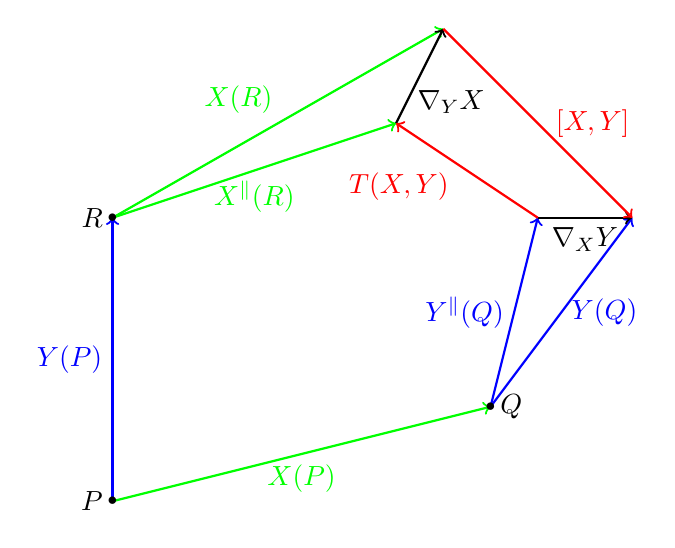
\begin{tikzpicture}[scale = 1.2]
                        \draw[->,thick,green] (0,0) -- (4,1) node[midway,below]{$X(P)$};
                        \draw[->,thick,green] (0,3) -- (3,4) node[midway,below]{$X^{\parallel}(R)$};
                        \draw[->,thick,green] (0,3) -- (3.5,5) node[midway,left=0.5cm,above]{$X(R)$};
                        \draw[->,thick,blue] (0,0) -- (0,3) node[midway,left]{$Y(P)$};
                        \draw[->,thick,blue] (4,1) -- (4.5,3) node[midway,left]{$Y^{\parallel}(Q)$};
                        \draw[->,thick,blue] (4,1) -- (5.5,3) node[midway,right]{$Y(Q)$};
                        \draw[->,thick] (4.5,3) -- (5.5,3) node[midway,below]{$\nabla_X Y$};
                        \draw[->,thick] (3,4) -- (3.5,5) node[midway,right=0.4cm,below=0.05cm]{$\nabla_Y X$};
                        \draw[->,thick,red] (3.5,5) -- (5.5,3) node[midway,right=0.1cm]{$[X,Y]$};
                        \draw[->,thick,red] (4.5,3) -- (3,4) node[midway,below=0.2cm  ,left=0.1cm]{$T(X,Y)$};
                        \draw (0,0) node[scale = 0.7]{$\bullet$};
                        \draw (4,1) node[scale = 0.7]{$\bullet$};
                        \draw (0,3) node[scale = 0.7]{$\bullet$};
                        \draw (0,0) node[below,left]{$P$};
                        \draw (4,1) node[below,right]{$Q$};
                        \draw (0,3) node[below,left]{$R$};
                    \end{tikzpicture}
                    \caption{Parallélogramme d'équipollence dans un espace courbe}
                    \label{fig:my_label}
                \end{figure}
                
                En relativité générale, nous avons
                \begin{equation}
                    T^\mu_{\nu\rho} = \Gamma^\mu_{\nu\rho} - \Gamma^\mu_{\rho\nu}
                \end{equation}
                Et comme $\Gamma^\rho_{\mu\nu} = \Gamma^\rho_{\nu\mu}$, $T^\mu_{\nu\rho} = 0$. C'est-à-dire que c'est une connexion de torsion nulle.
                
            \subsection{Théorème fondamental de la géométrie riemanienne}
            
                Depuis le début du cours, nous avons écrit $\Gamma^\rho_{\mu\nu}$ pour les symboles de Christoffel, ceci  a en fait été fait en prédiction du résultat qui suit. La notation des symboles de Christoffel qui est souvent utilisée est
                \begin{equation*}
                    \chris{\rho}{\mu}{\nu}\equiv
                    \Gamma^\rho_{\mu\nu}
                \end{equation*}
                et les symboles $\Gamma$ sont réservés à une connexion bien particulière qui est appellée la connexion de Levi-Civita. Nous allons voir que le théorème fondamentale de la géométrie riemannienne affirme que ces deux objets sont les mêmes. Toutefois, il est important de garder à l'esprit que ces deux objets ont a priori des origines différentes. Les symboles de Christoffel sont des coefficients qui apparaissent dans l'équation du mouvement d'une particule test. Ils sont définis comme
                \begin{equation}
                    \chris{\rho}{\mu}{\nu}~\hat{=}~
                    \frac{1}{2}g^{\mu\theta}\left( \p_\nu g_{\rho\theta}+\p_\rho g_{\nu\theta}-\p_\theta g_{\rho\nu} \right).
                \end{equation}
                Une connexion est une quantité qui porte la notion d'équipollence dans les espaces courbes. D'après les principes de la relativité générale, on peut imposer certaines condition à la connexion que nous utilisons (préservation de la métrique $g$ et torsion nulle). La connexion de Levi-Civita est l'unique connexion qui satisfait ces conditions.\\
            
                \begin{thm}[fondamental de la géométrie riemannienne]\begin{leftbar}
                    Sur une variété riemannienne $(\M,g)$, il existe une unique connexion de torsion nulle préservant la métrique. On l'appelle la \textit{connexion de Levi-Civita} telle que
                    \begin{equation}
                        \chris{\rho}{\mu}{\nu}=\Gamma^\rho_{\mu\nu}
                    \end{equation}
                \end{leftbar}\end{thm}
                
                \begin{proof}${}$\\
                    Soit une variété $\M$ munie d'une métrique $g$ et considérons une connexion $\nabla$ sur le fibré tangent $T\M$.
                    Cette démonstration se fait en plusieurs étapes.
                    \begin{enumerate}[label = \textit{\roman*)}]
                            \item Montrons que la condition de connexion préservant la            métrique est équivalente à la condition
                                \begin{equation}
                                    \nabla_\mu g_{\nu\rho}.
                                \end{equation}
                                Soient $3$ champs vectoriels sur $\M$ notés $X,Y$ et $V$. SI la connexion $\nabla$ préserve la métrique $g$, 
                                \begin{equation}
                                    \nabla_Vg(X,Y) = 0
                                \end{equation}
                                si $\nabla_V X = 0$ et $\nabla_V Y = 0$. Or de part la règle de Leibniz que nous avons déjà montrée,
                                \begin{align}
                                    0 &= \nabla_Vg(X,Y) \\
                                    &= V^\kappa \nabla_\kappa g(X,Y)\\
                                    &= V^\kappa(\nabla_\kappa g)(X,Y) + V^\kappa g( \nabla_\kappa X,Y) + V^\kappa g(X, \nabla_\kappa Y)\\
                                    &= V^\kappa(\nabla_\kappa g)(X,Y) + \underbrace{g(V^\kappa \nabla_\kappa X,Y)}_{0} +  \underbrace{g(X, V^\kappa\nabla_\kappa Y)}_{0}\\
                                    &= V^\kappa X^\mu Y^\nu \nabla_\kappa g_{\mu\nu}
                                \end{align}
                                Et particulier, si $V^\kappa = \delta^\kappa_\alpha,X^\mu = \delta^\mu_\beta$ et $Y^\nu = \delta^\nu_\sigma$, on obtient bien
                                \begin{equation}
                                    \nabla_\alpha g_{\beta\sigma} = 0.
                                \end{equation}
                                
                            \item Montrons que, les coefficients $\Gamma^\rho_{\mu\nu}$ d'une connexion $\nabla$ compatible avec la métrique (i.e. qui préserve la métrique), sont donnée par 
                            \begin{equation}
                                \Gamma^\rho_{\mu\nu} = \chris{\rho}{\mu}{\nu}+
                                K\indices{_\mu^\rho_\nu}
                            \end{equation}
                            où
                            \begin{equation}
                                K\indices{_\mu^\rho_\nu} = \frac{1}{2}\left( T\indices{^\rho_\mu_\nu}+T\indices{_\mu^\rho_\nu} + T\indices{_\nu^\rho_\mu} \right)
                            \end{equation}
                            est appelé le \textit{tenseur de contorsion}. Au préalable, notons que 
                            \begin{align}
                                -\nabla_{\lambda}g_{\mu\nu} &= -\p_\lambda g_{\mu\nu}+\Gamma^\kappa_{\lambda\mu}g_{\kappa\nu}+\Gamma^\kappa_{\lambda\nu}g_{\mu\kappa}\\
                                \nabla_{\mu}g_{\lambda\nu} &= \p_\mu g_{\lambda\nu}-\Gamma^\kappa_{\mu\lambda}g_{\kappa\nu}-\Gamma^\kappa_{\mu\nu}g_{\lambda\kappa}\\
                                \nabla_{\nu}g_{\lambda\mu} &= \p_\nu g_{\lambda\mu}-\Gamma^\kappa_{\nu\lambda}g_{\kappa\mu}-\Gamma^\kappa_{\nu\mu}g_{\lambda\kappa}
                            \end{align}
                            Nous avons que si $\nabla$ préserve la métrique alors $\nabla_{\alpha}g_{\mu\nu} = 0$. En supposant que la métrique est bien conservée, nous avons donc
                            \begin{align}
                                 0 &=  -\nabla_{\lambda}g_{\mu\nu}+ \nabla_{\mu}g_{\lambda\nu}+ \nabla_{\nu}g_{\lambda\mu}\\
                                 &= \left(\Gamma^\kappa_{\lambda\mu}g_{\kappa\nu} -\Gamma^\kappa_{\mu\lambda}g_{\kappa\nu}\right) +\left(\Gamma^\kappa_{\lambda\nu}g_{\mu\kappa} -\Gamma^\kappa_{\nu\lambda}g_{\kappa\mu}\right)\\
                                 &\hspace{0.4cm}+\left(-\Gamma^\kappa_{\mu\nu}g_{\lambda\kappa}-\Gamma^\kappa_{\nu\mu}g_{\lambda\kappa}\right) + \left( -\p_\lambda g_{\mu\nu}+\p_\mu g_{\lambda\nu} + \p_\nu g_{\lambda\mu}\right)\\
                                 &= T^\kappa_{~\lambda\mu}g_{\kappa\mu}+T^\kappa_{~\lambda\nu}g_{\nu\kappa}-2\Gamma^\kappa_{~(\mu\nu)}g_{\lambda\kappa} + \left( -\p_\lambda g_{\mu\nu}+\p_\mu g_{\lambda\nu} + \p_\nu g_{\lambda\mu}\right)
                            \end{align}
                            Multiplions de chaque coté par $g^{\sigma\lambda}$ et notons que
                            \begin{equation} g^{\sigma\lambda}\Gamma^\kappa_{~(\mu\nu)}g_{\lambda\kappa} = \delta^\sigma_\kappa
                            \end{equation}
                            Ce qui permet d'obtenir l'expression suivante pour $\Gamma^\kappa_{~(\mu\nu)}$:
                            \begin{align}
                                \Gamma^\kappa_{~(\mu\nu)} &= \frac{1}{2}g^{\sigma\lambda}\left( -\p_\lambda g_{\mu\nu}+\p_\mu g_{\lambda\nu} + \p_\nu g_{\lambda\mu}\right)+\frac{1}{2}T^\kappa_{~\lambda\mu}g^{\sigma\lambda}g_{\kappa\mu}+\frac{1}{2}T^\kappa_{~\lambda\nu}g^{\sigma\lambda}g_{\nu\kappa}\\
                                &= \chris{\kappa}{\mu}{\nu}+\frac{1}{2}\left( T\indices{_\nu^\kappa_\mu}+T\indices{_\mu^\kappa_\nu} \right)\\
                                &= \chris{\kappa}{\mu}{\nu} + T\indices{_{(\nu}^\kappa_{\mu)}}
                            \end{align}
                            Enfin,
                            \begin{align}
                                 \Gamma^\sigma_{~\mu\nu} &=  \Gamma^\sigma_{~(\mu\nu)}+ \Gamma^\sigma_{~[\mu\nu]}\\
                                 &= \chris{\sigma}{\mu}{\nu} + T\indices{_{(\nu}^\sigma_{\mu)}} + \frac{1}{2}T^\sigma_{~\mu\nu}\\
                                 &=  \chris{\sigma}{\mu}{\nu}+\underbrace{\frac{1}{2}\left( T\indices{_\nu^\kappa_\mu}+T\indices{_\mu^\kappa_\nu} +T^\sigma_{\mu_\nu}\right)}_{K\indices{_\mu^\sigma_\nu}}
                            \end{align}
                        \item La dernière étape est de montrer l'unicité et l'existence grâce aux deux premières étapes. Soit une connexion $\nabla'$ sur $(\M,g)$ telle que $\nabla'g = 0$. Par l'étape précédente,
                        \begin{equation}
                        \widetilde{\Gamma}^\lambda_{\mu\nu}=\chris{\lambda}{\mu}{\nu}+K\indices{_\mu^\lambda_\nu}
                        \end{equation}
                        Définissons la connexion
                        \begin{equation}
                            \Gamma^\lambda_{\mu\nu} = \widetilde{\Gamma}^\lambda_{\mu\nu} + A^\lambda_{\mu\nu}.
                        \end{equation}
                        C'est bien une connexion à condition que $A^\lambda_{\mu\nu}$ soient les composantes d'un tenseur de type $(1,2)$. Supposons que le changement de coordonnées de $x$ à $x'$ se fait par l'intermédiaire que la matrice jacobienne $J$. Dans ce cas,
                        \begin{equation}
                            \Gamma' = J^{-1}JJ\Gamma + \text{anomalies}
                        \end{equation}
                        Nous utilisons bien une notation, il ne faut pas considérer le produit des matrices $J$ directement. De plus,
                        \begin{equation}
                            \widetilde{\Gamma}' = J^{-1}JJ\Gamma + \text{anomalies}
                        \end{equation}
                        où les "anomalies" sont les mêmes. Ceci implique que $\widetilde{\Gamma}-\Gamma$ est bien un tenseur car
                        \begin{equation}
                            (\widetilde{\Gamma}'-\Gamma') = J^{-1}JJ(\widetilde{\Gamma}-\Gamma).
                        \end{equation}
                        Il suffit de poser $A^\lambda_{\mu\nu}=-K\indices{_\mu^\lambda_\nu}$. Nous avons construit une connexion
                        \begin{equation}
                            \chris{\lambda}{\mu}{\nu}=\Gamma^\lambda{\mu\nu}
                        \end{equation}
                        qui est unique car $\chris{\rho}{\mu}{\nu}$ est définit univoquement à partir de la métrique.
                    \end{enumerate}
                \end{proof}
                
                \begin{rmk}
                    On parle de géométrie riemannienne mais il s'agit en fait de géométrie pseudo-riemannienne car la variété de l'esapce-temps est munie d'une pseudo-métrique.
                \end{rmk}
                
                On conclu que le champ de gravitation est décrit par la métrique de l'espace-temps, c'est-à-dire par la géométrie de l'espace-temps.
            
        \section{Fibré vectoriel, section et connexion}
        
            \subsection{Section et fibre}
        
                Soit une variété différentiable $\M$. On veut généraliser la notion quantité physique (champ scalaire, champ vectoriel, champ tensoriel, champ spinoriel, etc). Prenons par exemple un champ scalaire. Il est claire que l'ensemble des valeur possible de champs doit former un espace vectoriel. Une quantité scalaire correspond donc en fait à une application sur l'espace-temps à valeur de $\mathbb{R}$. Ou de manière générale, une quantité physique est associée à une application dans un certain espace vectoriel.\\
                
                On voudrait associer à chaque point $P$ de $\M$, un espace vectoriel. Pour commencer, on se limite au cas particulier de l'esapce tangent.
                
                \begin{defn}
                    Le fibré tangent $T\M$ d'une variété différentiable $\M$ est l'ensemble
                    \begin{equation}
                        T\M = \bigcup_{P\in\M}T_P\M = \bigcup_{P\in\M}\left\{ (P,X)|P\in\M, X\in T_P\M \right\}
                    \end{equation}
                    muni de la projection
                    \begin{equation}
                    \pi:\left(
                    \begin{array}{ccc}
                        T\M & \longrightarrow & \M \\
                        (P,X) & \longmapsto & P
                    \end{array}
                    \right).
                    \end{equation}
                \end{defn}
                
                Une propriété remarquable du fibré tangent est qu'il lui-même être vu comme un variété.
                
                \begin{prop}\begin{leftbar}
                    Si $\M$ es une variété différentiable de dimension $n$ alors le fibré tangent $T\M$ admet une structure de variété différentiable de dimension $2n$ telle que
                    \begin{enumerate}[label = \textit{\roman*)}]
                        \item la projection $\pi:T\M\to\M$ ets différentiable
                        \item chaque fibre $\pi^{-1}(P)$ est difféomorphe à $\mathbb{R^{n}}$ pour tout $P\in\M$
                    \end{enumerate}
                \end{leftbar}\end{prop}
                
                Le fibré tangent permet d'associer un espace vectoriel à chaque point de la variété, l'espace vectoriel est ici le cas particulier de l'espace tangent. L'espace tangent étant naturellement associé à un point de la variété cette notion est assez naturelle. On peut généraliser ce principe pour n'importe quel type d'espace vectoriel, plus seulement l'espace tangent. On appelle ca le fibré vectoriel.
                
                \begin{defn}
                    Un \textit{fibré vectoriel} réel $\F$ de dimension $k$ sur la variété différentiable $\M$ est de projection $\pi:\F\to\M$ est une variété différentiable telle que pour tout $P\in\M$ il existe un voisinage $U\subset\M$ autour de $P$ tel que $\pi^{-1}(U)$ est difféomorphe à $U\times \mathbb{R}^k$ avec les propriétés suivantes
                    \begin{enumerate}[label = \textit{\roman*)}]
                        \item le diagramme suivant commute\\
                        %\begin{equation*}
                        %    \begin{CD}
                        %        S^{\mathcal{W}_\Lambda}\otimes T @>j>> T\\
                        %        @VVV @VV{\End P}V\\
                        %        (S\otimes T)/I @= (Z\otimes T)/J
                        %    \end{CD}
                        %\end{equation*}
                        où $\varphi_U$ est un difféomorphisme et $\pi_1$ est la projection sur le premier facteur.
                        \item toute composition $\varphi_V\circ\varphi_U^{-1} : (U\cap V)\times \mathbb{R}^k\to (U\cap V)\times \mathbb{R}^k$ où $U$ et $V$ sont disjoints, est linéaire en le second facteur.
                    \end{enumerate}
                \end{defn}
                
                La première propriété a pour but d'assurer que la projection $\pi:E\to\M$ est différentiable. La second propriété implique que la structure d'espace vectoriel est conservée par les applications $\varphi_V\circ\varphi_U^{-1}$. On peut voir $\F$ comme une famille d'espace vectoriels réels de dimension $k$ paramétrisée par $\M$.\\
                
                L'espace vectoriel qui est associé à un point $P\in\M$ est appelé la fibré en ce point. L'ensemble des fibres forme donc le fibré vectoriel.
                
                \begin{defn}
                    Soit un fibré vectoriel $\F$ de projection $\pi:\F\to\M$. Une \textit{section} de ce fibré vectoriel est une application différentiable $s:M\to\F$ telle que $\pi\circ s = id$ sur $\M$.
                \end{defn}
                
                On peut définir plus rigoureusement toute une série de termes.
                \begin{defn}${}$
                    \begin{itemize}[label = \textbullet]
                        \item un \textit{champ scalaire} est une section pour $\F_P = \mathbb{R}$
                        \item un \textit{champ vectoriel} est une section du fibré tangent
                        \item un \textit{champ tensoriel} est une section pour $\F_P = T_P^{(p,q)}\M$.
                        \item un \textit{champ de $1$-formes} est une section pour $\F_P = \Omega^1(\M)$
                    \end{itemize}
                \end{defn}
                
                Notons que ce formalisme n'est pas valable que pour la relativité générale mais aussi dans d'autres théories.
                
                \begin{exmp}${}$
                    \begin{itemize}[label = \textbullet]
                        \item pour mécanique quantique : $\F_P = \mathbb{C}$ et les sections sont les fonctions d'onde
                        \item pour le modèle standard des interactions fondamentales : les sections sont des champs quantiques de matière
                    \end{itemize}
                \end{exmp}
                
                \begin{defn}
                    Un \textit{fibré principal} est un fibré qui est aussi un groupe.
                \end{defn}
                
                Dans notre cas nous aurons souvent $\F_P = T_P^{(p,q)}\M$ mais les discussions qui suivent ne dépendent pas de ce choix.\\
                
                Notons que les fibres existent indépendemment de $\M$. Pour tout point $P\in\M$, on peut toujours se donner une base $\{e_a(P)\}$ de $\F_P$. De cette manière, $s(P)$ peut ere développé sur cette base comme
                \begin{equation}
                    s(P) = s^a(P)e_a.
                \end{equation}
                Si on a une matrice de changement de base $M$ qui permet de passer de la base $\{e_a(P)\}$ à une nouvelle base $\{e'_a(P)\}$ comme $e_a = M^b_{~~a} e'_b$, alors
                \begin{equation}
                    s'^a = M^a_{~~b}s^b
                \end{equation}
                
                Ce genre de transformation change peut-être la forme de que grandeur physique en tant que telle mais la physique reste la même. On sous-entend par là que, comme les lois de la physique ne dépendent des sections elle-mêmes, la manière dont on écrit ces sections ne change rien. Pour pouvoir décrire une section, il faut spécifier une base mais ce choix ne joue aucun rôle fondamental. On a discuté l'exemple d'un changement de base dans $\F_P$, ce qui correspond en fait à un changement de référentiel, mais on peut en fait s'autoriser toute une série de transformations plus générale encore cela.
                
                \begin{defn}
                    Soit $\{e_a(P)\}$ une base de $\F_P$ et $s = s^a(P)e_a$ une section, on appelle \textit{transformation de jauge} les transformations de type
                    \begin{equation}
                    s'^a = M^a_{~~b}s^b
                    \end{equation}
                    où $M\in G\subset GL(dim(\F_P)\mathbb{R})$. $G$ est appelé le \textit{groupe de structure du fibré} (ou \textit{groupe de jauge}).
                \end{defn}
                
                Les transformations de jauge décrivent les fameuse symétrie de jauge qui, comme nous l'avons mentionné précédemment, ne sont en fait pas des symétries à proprement parlé.
                
                \begin{exmp}
                    Prenons un exemple en mécanique quantique. On a $\F_P = \mathbb{C}$ et $G = U(1)$. Soit une fonction d'onde en $P$ $\psi|_P$, la fonction d'onde
                    \begin{equation}
                        \psi'|_P = e^{i\alpha}\psi|_P
                    \end{equation}
                    est alors équivalent pour tout $\alpha\in\mathbb{R}$.
                \end{exmp}
                
                Pour reformuler, en chaque point de l'espace-temps, on a un espace vectoriel qui contient les quantités physiques. Sur cet espace vectoriel, on s'autorise des transformations de jauge. Si l'on décide de spécifier un vecteur dans une base ou dans une autre, cela na change rien, le vecteur a une existence intrinsèque, sans quelconque base qui soit. Les transformations de jauge implémentant cette redondance.
            
            \subsection{Dérivation de section}
            
                Maintenant que ces notions sont établies, il est nécessaire de définir une notion de dérivée pour les sections. Soit $s$ une section, alors si $P,Q\in\M$, on pourrait être tenter de définir
                \begin{equation}
                    \nabla_\mu s~ dx^\mu = s(Q)-s(P)
                \end{equation}
                 mais $s(P)\in\F_P$ et $s(Q)\in\F_Q$ et soustraire des vecteurs qui ne sont pas au même point n'a pas de sens. En géométrie euclidienne ce problème n'existe pas car l'équipollence des vecteurs permet de pouvoir ramener n'importe quels vecteurs au même point. Comme l'espace de la géométrie euclidienne est plat, les vecteurs ne changent pas quand on les translate. Dans notre cas, il faut tenir compte de la courbure de l'espace pour pouvoir transformer les vecteurs correctement quand on les ramènes au même point, c'est ce rôle que joue les symboles de connexion. Considérons une sphère et deux vecteurs $v_1$ et $v_2$ et deux points différent cette sphère. Pour pourvoir soustraire ces vecteurs, il faut ramener $v_2$ au même point que $v_1$ (ou l'inverse). Si l'on fait juste une translation de $v_2$ on perd les propriétés du vecteurs. Par exemple, si $v_2$ est tangent à la sphère, le vecteur résultant ne le sera plus. Il faut adapté la notion de translation sur la sphère en tenant compte de la courbure. S'il on connaît comment s'exprime un vecteur "bien translaté" en fonction du vecteur d'origine dans une base donnée c'est bon. Les coefficients de la combinaison linéaire jouerais le rôle de connexion (symboles de connexion). Il est clair que ces symboles sont intrinsèque à la surface considérée, ici la sphère. L'idée est la même pour l'espace-temps. En d'autres termes, cet exercice de transport parallèle dans l'espace-temps doit être fait pas un certain isomorphisme. Il faut donc se donner un isomorphisme entre fibres $\F_P$ et $\F_Q$ "proches" (lorsque $P$ et $Q$ sont proches). Cet isomorphisme donnera la notion de transport parallèle. Faisons une tentative.
                 
                 \begin{defn}
                    Soit $\S_{P\to Q}$ l'\textit{opérateur de transport parallèle infinitésimal} un isomorphisme entre $\F_P$ et $\F_Q$.
                 \end{defn}
                 
                 D'après le raisonnement expliqué précédemment, on a alors
                 \begin{equation}\label{eq:derivsec}
                     \nabla_\mu s^a~dx^\mu = s^a(Q)-\left(\S_{P\to Q}(P)\right)^a
                 \end{equation}
                 et, par définition de dérivée covariante, on obtient
                 \begin{align}
                     \left(\S_{P\to Q}(P)\right)^a &= s^a(Q) + \nabla_\mu s^a~dx^\mu\\
                     &= s^a(Q) - \Gamma^a_{\mu b}~ s^b(P) ~dx^\mu
                 \end{align}
                 Si l'on utilise la notation $\Gamma_\mu$ pour le tenseur d'ordre deux de composantes $\Gamma^a_{\mu b}$, 
                 \begin{equation}
                     \S_{P\to Q}(P) = \mathbb{1} - \Gamma_\mu~dx^\mu
                 \end{equation}
                 Pour finir, s'il on prend $P = x$ et $Q = x+dx$, l'équation \ref{eq:derivsec} devient
                 \begin{align}
                      \nabla_\mu s^a~dx^\mu &= s^a(x+dx)-\left(\S_{P\to Q}(x)\right)^a\\
                      &= s^a(x+dx)-s^a(x)+\Gamma^a_{\mu b}s^b~dx^\mu
                 \end{align}
                 et donc lorsque $dx\to0$,
                 \begin{equation}
                     \nabla_\mu s^a = \p_\mu s^a+\Gamma^a_{\mu b}s^b.
                 \end{equation}
                 On voit bien que les $\Gamma^a_{\mu b}$ portent la notion d'équivalence de vecteur pour un espace courbe de métrique $g$. \\
                 
                 Après cette approche intuitive, voyons maintenant une approche plus axiomatique de la même notion.
                 
                 \begin{defn}
                    On note $\Sigma^p$ l'espace des $p$-formes à valeur dans les sections.
                 \end{defn}
                 
                 Notons que, d'après cette définition, $\Sigma^0$ est l'espace des sections elles-mêmes. Nous avons donc
                 \begin{equation}
                    \Sigma^p = \Omega^p(\M)\otimes\Sigma^0.
                \end{equation}
                
                \begin{exmp}
                    Soit $h\in \Sigma^p$, alors
                    \begin{equation}
                        h = \frac{1}{p'}\omega^a_{\mu_1\dots\mu_p}~dx^{\mu_1}\wedge\dots\wedge dx^{\mu_p}\otimes e_a.
                    \end{equation}
                    
                    Si $p=1$, $h\in\Sigma^1$ et si $x\in T_P\M$ alors $h(x)\in\Sigma^0$ car 
                    \begin{equation}
                        h = h^a_\mu~dx^\mu\otimes e_a
                    \end{equation}
                    et donc
                    \begin{equation}
                        h(x) = h^a_\mu x^\mu e_a.
                    \end{equation}
                \end{exmp}
                
                \begin{defn}
                    Une \textit{connexion} est une application
                    \begin{equation}
                    \nabla:\left(
                    \begin{array}{ccc}
                        \Sigma^0 & \longrightarrow & \Sigma^1 \\
                        f & \longmapsto & \nabla f
                    \end{array}
                    \right)
                    \end{equation}
                    telle que 
                    \begin{equation}
                        \nabla(fs) = df\otimes s+f\nabla s
                    \end{equation}
                    pour toute fonction $f:\M\to\mathbb{R}$ et pour tout $s\in\Sigma^0$.
                \end{defn}
                
                Notons que $\nabla$ est à valeur dans $\Sigma^1$ var la dérivation est fonctionnelle. Si $S\in T_P\M$,
                \begin{align}
                    \nabla_X s &= (\nabla s)(X)\\
                    &= X^\mu\nabla s(\p_\mu)\\
                    X^\mu\nabla_\mu s
                \end{align}
             
                Soit $\{e_a^{(P)}\}$ une base de $\F_P$ alors
                \begin{align}
                    \nabla s &= \nabla(s^a e_a)\\
                    &= ds^a\otimes e_a+s^a\nabla e_a
                \end{align}
            donc $\nabla s$ est fixée, quelque soit $s$, si l'on connaît $\nabla e_a$. 
            \begin{defn}
                Les \textit{$1$-forme de la connexion} sont les  $1$-forme $\Gamma^b_a\in\Omega^1(\M)$ à valeur dans l'espace des sections qui permettent la décomposition
                \begin{equation}
                    \nabla e_a = \Gamma^b_a \otimes e_b.
                \end{equation}
                On note $\Gamma$ la matrice des $1$-forme de la connexion.
             \end{defn}
             
            D'après ce que l'on a vu ci-dessus,
            \begin{equation}
                 \Gamma^a_b = \Gamma^a_{\mu b}~dx^\mu
            \end{equation}
            on voit bien que les indices $a,b$ et $\mu$ jouent des rôles très différents. Finalement, nous retrouvons la même formule que dans notre approche intuitive du problème.
            \begin{align}
                 \nabla s(X) &= \nabla_X s\\
                 &= ds^a(X)e_a+\Gamma^a_b(X)e_b\\
                 &= X^\mu(\p_\mu s^a+\Gamma^a_{\mu b}s^b)e_a
            \end{align}
             
            \begin{prop}\begin{leftbar}
                    La dérivée covariante d'une section $s = s^a e_a$ est donnée par
                    \begin{equation}
                        \nabla_\mu s^a = \p_\mu s^a+\Gamma^a_{\mu b}s^b
                    \end{equation}
            \end{leftbar}\end{prop}
             
            Que se passe-t-il sous un changement de base ? Ou de manière plus générale, que se passe-t-il sous une transformation de jauge ? Pour faire le cas générale, on va considérer un changement de base uniquement pour les fibres et pas dans l'esapce tangent. On verra plus après le cas particulier où les fibres sont des espaces tangents qu'est le notre.
            
            \begin{prop}\begin{leftbar}
                Sous un changement de coordonnées du type
                \begin{align}
                    e_a' &= N_a^{~b}~e_b \\
                    s'^a &= M^a_{~b} ~s^b
                \end{align}
                 avec $M\in G$ et $N = (M^{-1})^T$. Nous avons
                 \begin{equation}
                     \Gamma' = M\Gamma M^{-1} + MdM^{-1}
                 \end{equation}
            \end{leftbar}\end{prop}
        
            \begin{proof}
                On a 
                \begin{equation}
                    (\nabla s)^a = ds^a + \Gamma^a_b s_b.
                \end{equation}
                D'une part, 
                \begin{align}
                    (\nabla s)'^a &= ds'^a +  \Gamma'^a_{~b} s'_b \\
                    &= d(M^a_{~b} ds^b) + \Gamma'^a_{~b} M^b_{~c}s^c \\
                    &= M^a{~b}ds^b + dM^a_{~c}s^b + \Gamma'^a_{~b} M^b_{~c}s^c
                \end{align}
                et d'autre part,
                \begin{align}
                    (\nabla s)'^a &= M^a_{~b}(\nabla s)^b \\
                    &=  M^a_{~b}\left( ds^b+\Gamma^b_{~c}s^c \right)
                \end{align}
                ce qui entraîne que
                \begin{align}
                     M^a_{~b}\Gamma^b_{~c}s^c &=  dM^a_{~c}s^b + \Gamma'^a_b M^b_{~c}s^c\\
                     \Leftrightarrow \qquad (M\Gamma)^a_{~c}s^c &= dM^a_{~c}s^b + (\Gamma'M)^a_{~c}s^c\\ 
                     \Leftrightarrow \qquad M\Gamma &= \Gamma'M - dM
                \end{align}
                ou encore
                \begin{align}
                    \Gamma' &= M\Gamma M^{-1}-(dM)M^{-1}\\
                    &= M\Gamma M^{-1} + MdM^{-1}
                \end{align}
                Le dernière égalité venant du fait que $MM^{-1} = \mathbb{1}$ et donc 
                \begin{equation}
                    dM\cdot M^{-1} + M\cdot dM^{-1} = 0.
                \end{equation}
            \end{proof}
        
            Remarquons que, composante par composante, la loi de transformation des $\Gamma$ donne 
            \begin{equation}
                \Gamma'^{a}_{~b} = M^a_{~c}\Gamma^c_{~d}(M^{-1})^d_{~b}+M^a_{~c}(dM^{-1})^c_{~b}
            \end{equation}
            ce qui montre bien que $\Gamma$ n'est pas une $1$-forme à valeur dans $F\otimes F^* = End(F)$.
            \begin{equation}
                \Gamma\notin \Omega^1(\M)\otimes F \otimes F^*
            \end{equation}
            Toujours d'après ce que l'on vient de voir, si $\Gamma = \Gamma_\mu~dx^\mu$,
            \begin{equation}
                \Gamma'_{\mu} = M\Gamma M^{-1} + M\p_\mu M^{-1}.
            \end{equation}
            Notons bien que nous effectué un changement de base sur la fibre mais que nous avons utilisé la même base de $\Omega^1(\M)$ pour développer $\Gamma'$ et $\Gamma$.\\
            
            Dans le cas particulier où $F_P : T_P\M$ et où le changement de base sur la fibre correspond à un changement de coordonnées, il est naturelle d'exprimer les $1$-forme $\Gamma$ dans la base $\{dx^\mu\}$ et les $1$-formes $\Gamma'$ dans la base $\{dx'^\mu\}$. Dans ce cas, $M^a{~b}$ devient $\pdv{x'^\mu}{x^\nu}$ et donc 
            \begin{equation}
                \gamma'^\mu_{~\nu} = \pdv{x'^\mu}{x^\rho}\pdv{x^\sigma}{x^\nu}\Gamma^\rho_{~\sigma} + \pdv{x'^\mu}{x^\theta}~d\left( \pdv{x^\theta}{x'^\nu} \right)
            \end{equation}
            On exprime $\Gamma$ et $\Gamma'$ comme suit.
            \begin{equation}
                \Gamma'^\mu_{~\nu} =  \Gamma'^\mu_{\kappa\nu}~dx'^\kappa \qquad ; \qquad  \Gamma^\rho_{~\sigma} =  \Gamma^\rho_{\xi\sigma}~dx^\xi
            \end{equation}
            On trouve donc 
            \begin{align}
                \Gamma'^\mu_{\kappa\nu}~dx'^\kappa &= \pdv{x'^\mu}{x^\rho}\pdv{x^\sigma}{x^\nu} \Gamma^\rho_{\xi\sigma}~dx^\xi + \pdv{x'^\mu}{x^\theta}\pdv{x^\theta}{x'^\nu}{x'^\kappa}~dx'^\kappa\\
                &= \pdv{x'^\mu}{x^\rho}\pdv{x^\sigma}{x^\nu} \Gamma^\rho_{\xi\sigma}\pdv{x^\xi}{x'^\kappa}~dx^\kappa + \pdv{x'^\mu}{x^\theta}\pdv{x^\theta}{x'^\nu}{x'^\kappa}~dx'^\kappa
            \end{align}
            En identifiant les coefficients devant les $dx'^\kappa$, on retrouve la loi de transformation de $\Gamma$.
            
            \begin{exmp}
                Si $G = U(1)$ et $F = \mathbb{C}$, alors $M = e^{i\alpha}$ et $\Gamma$ est une matrice $1\times1$ et donc
                \begin{align}
                    \Gamma' &= M\gamma M^{-1} + MdM^{-1} \\
                    &= \Gamma + e^{i\alpha}d(e^{i\alpha}) \\
                    &= \Gamma-i\alpha d\alpha
                \end{align}
                Dans une base des coordonnées,
                \begin{equation}
                    \Gamma'_\mu = \Gamma_\mu-i\alpha\p_\mu\alpha
                \end{equation}
                Dans le cas du potentiel vecteur électromagnétique, on trouve la transformation de jauge
                \begin{equation}
                    A'_\mu = A_\mu - \p_\mu\alpha.
                \end{equation}
                Et, 
                \begin{align}
                    \nabla_\mu\psi &= \p_\mu\psi + \Gamma_\mu \\
                    &= (\p_\mu+iA_\mu)\psi
                \end{align}
                C'est la dérive covariante d'un spinneur chargé. On verra que dans ce cas, la courbure est le champ électromagnétique. Le potentiel vecteur est à l'électromagnétisme ce que $\Gamma$ est à la relativité générale.
            \end{exmp}
            
            \begin{exmp}
                Dans le modèle standard des interactions fondamentales, $G$ est un groupe non-abélien :
                \begin{equation}
                    G = SU(3)\times SU(2)\times U(1)
                \end{equation}
                et $\Gamma = iA$ (c'est un élément de l'algèbre de Lie de $G$). Dans ce cas, on trouve
                \begin{equation}
                    A' = MAM^{-1}-iMdM^{-1}.
                \end{equation}
                C'est la transformation de jauge pour une théorie de jauge non-abélienne.
            \end{exmp}
        
        \section{Lignes droites et géodésiques}
        
            \begin{defn}
                Soit $(I,\gamma)$ une courbe $C^\infty$ dans $\M$, $I$ est  un intervalle ouvert de $\mathbb{R}$ et $\gamma:I\to\M$ une application $C^\infty$. Pour tout $\lambda\in I$, on définit un vecteur tangent à $\M$ au point $\gamma(\lambda)$, appelé \textit{vecteur tangent à la courbe} $\gamma$ en $\lambda$, on le note $\dot{\gamma}(\lambda)$.
                \begin{equation}
                    \dot{\gamma}:\left(
                    \begin{array}{ccc}
                        C^\infty(\M,\mathbb{R}) & \longrightarrow & \mathbb{R} \\
                        f & \longmapsto & \dot{\gamma}(\lambda)(f)
                    \end{array}
                    \right)
                    \end{equation}
                    où
                    \begin{equation}
                         \dot{\gamma}(\lambda)(f) ~\hat{=}~ \frac{d}{dt}f(\gamma(t))|_{t=\lambda}.
                    \end{equation}
            \end{defn}
            
            On voit bien que c'est un vecteur de l'espace tangent car $f\circ\gamma$ est une fonction $C^\infty$ et la dérivée $\frac{d}{dt}$ satisfait à la règle de Leibniz.
            
            \begin{rmk}
                Lorsque l'on a introduit la notion d'espace tangent, on a montré que les dérivée partielle en fonction des dérivées locales formaient une base de ce dernier. Cela veut dire qu'il est possible de développer l'expression d'un vecteur tangent à une courbe sur cette base. Cela se fait en faisant apparaître l'application de coordonnée dans l'expression puis en utilisant la chain rule. On peut montrer que tout vecteur tangent $X_P\in T_P\M$ en $P$ peut être considéré comme un vecteur tangent à une courbe passant par $P$. Cette caractérisation est non unique.
            \end{rmk}
            
            Nous noterons $x^\mu(\lambda)\equiv (x\circ \gamma)(\lambda)$ une courbe dans $\M$ de paramètre $\lambda$. Le vecteur tangent à cette courbe en $P$ est
                \begin{equation}
                    U^\mu = \frac{dx^\mu}{d\lambda}(P)
                \end{equation}
            ce n'est donc pas un champ de vecteur comme on l'a vu avant car ces vecteurs sont définis uniquement le long de la courbe. On vérifie facilement que c'est bien un vecteur.\\
            
            Comme $U^\mu$ n'est définit que le long de la courbe, la dérivée covariante $\nabla_X U^\mu\equiv X^\nu\nabla_\nu V^\mu$ n'est pas bien définie. On peut cependant définir correctement $\nabla_U U^\mu\equiv U^\nu\nabla_\nu V^\mu$. Nous avons alors
            \begin{align}
                \nabla_U U^\mu &= U^\nu\nabla_\nu V^\mu \\
                &= \frac{dx^\mu}{d\lambda}\p_\mu V^\nu + \Gamma^\nu_{\mu\rho}U^\mu U^\rho \\
                &= \frac{dU^\mu}{d\lambda} + \Gamma^\nu_{\mu\rho} U^\mu U^\rho
            \end{align}
            Ce résultat peut être généralisé à n'importe que tenseur défini le long d'une courbe $\mathscr{C}$.
            \begin{prop}\begin{leftbar}
                Soit une courbe $\mathscr{C}$ sur $\M$ de paramètre $\lambda$. Si $U$ est un vecteur tangent à $\mathscr{C}$, alors la dérivée d'un tenseur $t$ de type $(p,q)$ est
                \begin{equation}
                    \nabla_U t^{\mu_1\dots\mu_p}_{\nu_1\dots\nu_q} = \frac{dt^{\mu_1\dots\mu_p}_{\nu_1\dots\nu_q}}{d\lambda} + U^\mu(\Gamma_\mu t + \dots)
                \end{equation}
            \end{leftbar}\end{prop}
            
            \begin{proof}
                Il suffit de développer l'expression de la dérivée covariante de la même manière que précédemment.
            \end{proof}
            
            Les tenseurs $\nabla t$ sont définit le long de $\mathscr{C}$.\\
            
            Comment définir une ligne droite ? En géométrie euclidienne, la droite peut être définie comme étant le plus court chemin entre deux points. Cependant, la notion "plus court" dépend de la métrique dont dispose l'espace que l'on étudie. Le fait que le chemin le plus court entre deux points est une droite est une conséquence de la forme de la métrique euclidienne. Sur une sphère, les chemins les plus court sont des les grands cercles. Fondamentalement, on peut définir une droit comme étant une courbe dont le vecteur tangent ne change pas de direction. C'est-à-dire une courbe telle que
            \begin{equation}
                \nabla_U U = f(\lambda) U
            \end{equation}
            La notion de ligne droite dépend de la connexion de transport parallèle.\\
            
            Le membre de droite peut toujours être éliminé par un choix approprié de paramètre $\lambda$. Effectivement, supposons que $\lambda = \lambda(\lambda')$,
            \begin{align}
                \nabla_U U^\mu &= \frac{dU^\mu}{d\lambda} + \Gamma^\nu_{\mu\rho} U^\mu U^\rho \\
                &= \frac{d^2x^\mu}{d\lambda^2} + \Gamma^\nu_{\mu\rho} \frac{dx^\nu}{d\lambda}\frac{dx^\mu}{d\lambda} \\
                &= \left( \frac{d\lambda'}{d\lambda} \right)^2\frac{d^2x^\mu}{d\lambda'^2}+\frac{d^2\lambda'}{d\lambda^2}\frac{dx^\mu}{d\lambda'}+\left( \frac{d\lambda'}{d\lambda} \right)^2\Gamma^\mu_{\nu\rho} \frac{dx^\nu}{d\lambda'}\frac{dx^\mu}{d\lambda'}
            \end{align}
            d'autre part, 
            \begin{align}
                \nabla_U U^\mu &= f(\lambda) \frac{dx^\mu}{\lambda} \\
                &= \frac{d\lambda'}{d\lambda}f(\lambda)\frac{dx^\mu}{d\lambda'}
            \end{align}
            En égalant ces deux termes, on trouve
            \begin{equation}
                \left( \frac{d\lambda'}{d\lambda} \right)^2\frac{d^2x^\mu}{d\lambda'^2}+\frac{d^2\lambda'}{d\lambda^2}\frac{dx^\mu}{d\lambda'}+\left( \frac{d\lambda'}{d\lambda} \right)^2\Gamma^\mu_{\nu\rho} \frac{dx^\nu}{d\lambda'}\frac{dx^\mu}{d\lambda'} = \frac{d\lambda'}{d\lambda}f(\lambda)\frac{dx^\mu}{d\lambda'}
            \end{equation}
            donc
            \begin{equation}
                \frac{d^2x^\mu}{d\lambda'^2} + \Gamma^\mu_{\nu\rho} \frac{dx^\nu}{d\lambda'}\frac{dx^\mu}{d\lambda'} = 0
            \end{equation}
            si 
            \begin{align}
                \frac{d^2\lambda'}{d\lambda^2} &= \frac{d\lambda'}{d\lambda}f(\lambda)
            \end{align}
            et cette équation différentielle est toujours solvable. Il existe toujours une solution $\lambda'(\lambda)$.
            
            \begin{defn}
                Le paramètre permettant de réduire l'équation d'une droite à 
                \begin{equation}
                    \nabla_U U = 0
                \end{equation}
                est appelé \textit{paramètre affine}.
            \end{defn}
            
            \begin{prop}\begin{leftbar}
                Soient $\lambda_1$ et $\lambda_2$ deux paramètre affines pour une courbe $\mathscr{C}$. Il existe $\alpha,\beta\in\mathbb{R}$ tels que
                \begin{equation}
                    \lambda_1 = \alpha\lambda_2+\beta.
                \end{equation}
            \end{leftbar}\end{prop}
            
            Pour certaines courbe, le paramètre affine correspond à une quantité physique bien connue : le temps propre.
            
            \begin{defn}
                Une \textit{géodésique} est une courbe qui extrémalise la distance entre deux point.
            \end{defn}
            
            \begin{exmp}
                En géométrie euclidienne, la distance entre deux points $P$ et $Q$ est donnée par 
                \begin{equation}
                    L = \int_P^Q ds = \int_P^Q \sqrt{dx^2+dy^2}
                \end{equation}
                on peut alors montrer que les courbes satisfaisant $\delta L = 0$ sont les lignes droites.
            \end{exmp}
            
            \begin{exmp}
                Sur la sphère unité $S^2$, la distance est donnée par
                \begin{equation}
                    L = \int_P^Qds = \int_P^Q\sqrt{dr^1+d\theta^2+\sin^2\theta d\phi^2}
                \end{equation}
                en coordonnées sphériques. Les courbes qui extrémalisent cette distance sont les grands cercles (cercle issus de l'intersection d'un plan passant par le centre avec la sphère).
            \end{exmp}
            
            \begin{defn}
                En signature Minkowskienne, on considère 3 types de courbe :
                \begin{itemize}[label = \textbullet]
                    \item de \textit{genre temps} : si $g(t,t)<0$
                    \item de \textit{genre lumière} : si $g(t,t)=0$
                    \item de \textit{genre espace} : si $g(t,t)>0$
                \end{itemize}
            \end{defn}
            
            \begin{exmp}
                En relativité restreinte, la distance est donnée par
                \begin{equation}
                    S = -m\int_P^Qd\tau = -m\int_P^Q\sqrt{\eta_{\alpha\beta}dx^\alpha dx^\beta} = -m\int_P^Q\sqrt{1-v^2}dt
                \end{equation}
                où le signe "-" et le paramètre $m$ (masse) sont conventionnels. Les courbe qui minimisent la distance sont celles qui minimisent l'action $S$, c'est-à-dire les courbe pour lesquelles $v=0$.
            \end{exmp}
            
            \begin{thm}\begin{leftbar}
                Si $\Gamma$ est la connexion de Levi-Civita alors les lignes droites extrémalisent  la fonctionnelle temps propre entre deux points
                \begin{equation}
                    S = -m\int_P^Qd\tau
                \end{equation}
                pour les courbes de genre temps.
            \end{leftbar}\end{thm}
            
            \begin{proof}${}$\\
                Rappelons que, par définition du temps propre,
                \begin{align}
                    S &= -m\int_P^Q d\tau\\
                    &= -m\int_{\lambda_1}^{\lambda_2}\sqrt{-g_{\mu\nu}\dot{x}^\mu\dot{x}^\nu}d\lambda
                \end{align}
                où $\dot{x}^\mu = \frac{x^\mu}{d\lambda}$. Nous avons le lagrangien
                \begin{equation}
                    \mathcal{L} = \sqrt{-g_{\mu\nu}\dot{x}^\mu\dot{x}^\nu}.
                \end{equation}
                Il suit que
                \begin{align}
                    \pdv{\mathcal{L}}{x^\mu} &= -\frac{2}{\sqrt{2F}}\p_\mu g_{\nu\rho}\dot{x}^\mu\dot{x}^\nu \\
                    \pdv{\mathcal{L}}{\dot{x}^\mu} &= -\frac{2}{2\sqrt{F}}g_{\mu\nu}\dot{x}^\nu\\
                    \frac{d}{d\lambda}\pdv{\mathcal{L}}{\dot{x}^\mu} &= -\frac{g_{\mu\nu}\ddot{x}^\nu}{\sqrt{F}}-\frac{\p_\mu g_{\mu\nu} \dot{x}^\mu\dot{x}^\nu}{\sqrt{F}}-\frac{1}{2F^{\frac{3}{2}}}\frac{dF}{d\lambda}
                \end{align}
                Les équation d'Euler-Lagrange nous donnent alors
                \begin{equation}
                    \ddot{x}^\xi + \frac{1}{2}g^{\mu\xi}\underbrace{\left( \p_\rho g_{\mu\nu}+\p_\nu g_{\mu\rho} - \p_\mu g_{\nu\rho} \right)}_{\Gamma^\xi_{\nu\rho}}\dot{x}^\nu\dot{x}^\rho = f(\lambda)
                \end{equation}
                ou encore
                \begin{equation}
                    \nabla_U U^\mu = f(\lambda)U^\mu
                \end{equation}
            \end{proof}
            
            Notons que si l'on prend $\lambda = \tau$, alors $g(U,U) = -1 = -F$ et donc
            \begin{equation}
                \frac{dF}{d\lambda} = 0.
            \end{equation}
            On peut en conclure que le temps propre est un paramètre affine. En géométrie euclidienne, la paramètre affine est la abscisse curviligne.
            
            \begin{prop}\begin{leftbar}
                Si $U$ est le vecteur tangent le long d'un courbe, alors la quantité
                \begin{equation}
                    g(U,U) = g_{\mu\nu}U^\mu U^\nu
                \end{equation}
                où $U^\mu = \frac{dx^\mu}{d\lambda}$, est constante le long de cette courbe.
            \end{leftbar}\end{prop}
            
            \begin{proof}${}$\\
                Il suffit de remarquer que
                \begin{align}
                    \frac{d}{d\lambda}\left((g(U,U)\right) &= \nabla_U\left(g(U,U)\right) \\
                    &= \left(\nabla_Ug\right)(U,U) + g(\nabla_U U,U) + g(U,\nabla U) 
                \end{align}
                Les deux dernier termes s'annulent car $\lambda$ est un paramètre affine et le terme $\left(\nabla_Ug\right)(U,U)$ s'annule car la dérivée covariante réserve la métrique. On conclu que $g(U,U)$ ne dépend pas du paramètre $\lambda$.
            \end{proof}
            
            \begin{defn}
                Il existe trois familles de géodésiques qualitativement distinctes :
                \begin{itemize}[label = \textbullet]
                    \item $g(U,U)<0$ : \textit{géodésique de genre temps}, on peut alors normaliser la paramètre affine pour que $g(U,U) = -1$, le paramètre affine renormalisé est identifié avec le temps propre. Le principe d'équivalence implique que les lignes d'univers des particules soumises uniquement au champ de gravitation sont de genre temps.
                    \item $g(U,U)=0$ : \textit{géodésique de genre lumière}, le principe d'équivalence implique que ce sont les lignes d'univers des particules de masse nulle.
                    \item $g(U,U)>0$ : \textit{géodésique de genre espace}, on peut alors normaliser la paramètre affine pour que $g(U,U) = 1$, le paramètre affine renormalisé est l'abscisse curviligne le long de la géodésique.
                \end{itemize}
            \end{defn}
            
            \begin{prop}\begin{leftbar}
                Les géodésiques de genre temps extrémalisent l'action
                \begin{equation}
                    S = -m\int d\tau = -m\int \sqrt{g_{\mu\nu}\frac{dx^\mu}{d\lambda}\frac{dx^\nu}{d\lambda}}.
                \end{equation}
            \end{leftbar}\end{prop}
            
            Notons que cette action est invariante par changement de paramètre affine.\\
            
            La proposition précédente fait penser à une version de principe de moindre action. Voyons comment formuler un principe de moindre action alternatif à proprement parlé.\\
            
            Soit courbe de paramètre affine $\lambda$. Considérons l'action
            \begin{equation}
                \sigma = \int g_{\mu\nu}\dot{x}^\mu\dot{x}^\nu~d\lambda
            \end{equation}
            où $\dot{x}^\mu\equiv\frac{dx^\mu}{d\lambda}$. Cette action n'est pas invariante par changement de paramètre affine. Le lagrangien qui correspond à cette action est 
            \begin{equation}
                \mathscr{L} = g_{\mu\nu}\dot{x}^\mu\dot{x}^\nu
            \end{equation}
            
            \begin{prop}\begin{leftbar}
                Les équations d'Euler-Lagrange pour le lagrangien
                \begin{equation}
                \mathscr{L} = g_{\mu\nu}\dot{x}^\mu\dot{x}^\nu
                \end{equation}
                sont équivalentes à l'équation des géodésiques.
            \end{leftbar}\end{prop}
            
            \begin{proof}${}$\\
                Les équations d'Euler-Lagrange sont données par
                \begin{align}
                    \frac{d}{d\lambda}\pdv{\mathscr{L}}{\dot{x}^\mu} &= \pdv{\mathscr{L}}{x^\mu}\\
                    \Leftrightarrow\qquad 2\frac{d}{d\lambda}(g_{\mu\nu}\dot{x}^\nu) &= \p_\mu g_{\nu\rho}\dot{x}^\nu\dot{x}^\rho\\
                    \Leftrightarrow\qquad \p_\rho g_{\mu\nu}\dot{x}^\rho\dot{x}^\nu + g_{\mu\nu}\ddot{x}^\nu &= \frac{1}{2}\left( \p_\mu g_{\nu\rho}\dot{x}^\nu\dot{x}^\rho \right)
                \end{align}
                En multipliant la dernière équation par $g^{\mu\sigma}$, nous obtenons
                \begin{equation}
                    \ddot{x}^\sigma + \underbrace{g^{\mu\sigma}\left( \p_\rho g_{\mu\nu}+\p_\nu g_{\mu\rho} - \p_\mu g_{\nu\rho} \right)}_{2\Gamma^\sigma_{\nu\rho}}\dot{x}^\nu\dot{x}^\rho = 0\label{eq:calculgamma}
                \end{equation}
            \end{proof}
            
            Ce raisonnement nous donne une méthode facile pour le calcul des symboles $\Gamma$:
            \begin{enumerate}
                \item écrire le langrangien $\mathscr{L}$
                \item écrire les équation d'Euler-Lagrange
                \item lire les symboles $\Gamma$ sur ces équations
            \end{enumerate}
            
            \begin{exmp}
                Appliquons cette méthode dans le cas du plan euclidien décrit à l'aide des coordonnées polaires $(\rho,\theta)$. L'élément de distance est donné par 
                \begin{equation}
                    ds^2 = d\rho^2 + \rho^2d\theta^2.
                \end{equation}
                \begin{enumerate}
                    \item Le langragien est
                    \begin{equation}
                        \mathscr{L} = \dot{\rho}^2+\rho^2\dot{\theta}^2
                    \end{equation}
                    \item Écrivons les équation d'Euler-Lagrange pour chaque coordonnée.
                    \begin{align}
                        \frac{d}{d\lambda}\pdv{\mathscr{L}}{\dot{\rho}} &= \pdv{\mathscr{L}}{\rho}\\
                        \Leftrightarrow\qquad \frac{d}{d\lambda}\left( 2\dot{\rho} \right) &= 2\rho\dot{\theta}^2 \\
                        \Leftrightarrow\qquad \ddot{\rho} - \rho\dot{\theta}^2 &= 0
                    \end{align}
                    \begin{align}
                        \frac{d}{d\lambda}\pdv{\mathscr{L}}{\dot{\theta}} &= \pdv{\mathscr{L}}{\theta}\\
                        \Leftrightarrow\qquad \frac{d}{d\lambda}\left(2\rho^2\dot{\theta} \right) &= 0 \\
                        \Leftrightarrow\qquad \ddot{\theta}+\frac{2}{\rho}\dot{\rho}\dot{\theta} &= 0
                    \end{align}
                    Les équation obtenue sont 
                    \begin{subequations}
                    \begin{empheq}[left=\empheqlbrace]{align}
                        \Leftrightarrow\qquad \ddot{\rho} - \rho\dot{\theta}^2 &= 0 \\
                        \ddot{\theta}+\frac{2}{\rho}\dot{\rho}\dot{\theta} &= 0
                    \end{empheq}
                    \end{subequations}
                    Ce sont les équations des droites.
                    \item En comparant avec la formule \ref{eq:calculgamma}, on obtient
                    \begin{align}
                        \Gamma^\rho_{\theta\theta} &= -\rho\\
                        \Gamma^\theta_{\rho\theta} &= \Gamma^\theta_{\theta\rho} = \frac{1}{\rho}
                    \end{align}
                    Tout les autres symboles sont nuls.
                \end{enumerate}
            \end{exmp}
            
        \section{Courbure}
            
            Étant donné une métrique $g$ (i.e. un champ de gravitation), comme faire pour savoir s'il on affaire à la métrique de Minkowsky $\eta = \eta_{\mu\nu}dx^\mu dx^\nu$ dans un système de coordonnées compliquées ou alors à une métrique intrinsèquement différente associée à un champ de gravitation non-trivial. Dans le premier cas, il doit être possible de trouver un changement de variable astucieux pour retrouver la métrique de Minkowsky mais ce changement de variable n'est pas toujours facile à trouver, ce qui rend la distinction entre les deux cas peu évidente si l'on observe juste l'expression de la métrique. On cherche donc un autre moyen de différencier ces deux cas.
            
            \begin{exmp}
                Considérons le plan euclidien décrit à l'aide des coordonnées polaires $(\rho,\theta)$. L'élément de distance dans ces coordonnées est donné par 
                \begin{equation}
                    ds^2 = d\rho^2 + \rho^2d\theta^2.
                \end{equation}
                Le changement de variable
                \begin{subequations}
                    \begin{empheq}[left=\empheqlbrace]{align}
                        x &= \rho\cos\theta\\
                        y &= \rho\sin\theta
                    \end{empheq}
                \end{subequations}
                permet de retrouver l'expression
                \begin{equation}
                    ds^2 = dx^2+dy^2.
                \end{equation}
                De manière générale, ce genre de changement de varible est a priori très difficile à trouver.
            \end{exmp}
            
            Pour reformuler mathématiquement, on cherche à savoir s'il existe un système de coordonnées $x(z)$ tel que
            \begin{equation}
                g_{\mu\nu}(x) = \pdv{z^\alpha}{x^\mu}\pdv{z^\beta}{x^\nu}\eta_{\alpha\beta}.
            \end{equation}
            D'après le principe d'équivalence, on sait qu'il est toujours possible, pour tout $P\in\M$ de trouver un système de coordonnée locales tel que
            \begin{equation}
                \pdv{x^\mu}{z^\alpha_P}\pdv{x^\nu}{z^\beta_P}g_{\mu\nu}(P) = \eta_{\alpha\beta} + \order{z^2}
            \end{equation}
            Comme nous l'avons vu, il n'est , en générale, pas possible d'annuler les termes en $z^2$ (termes en $\p_\alpha\p_\beta g_{\gamma\delta}(P)$) car le nombre de contraintes (nombre d'invariants de courbure)
            \begin{equation}
                \mathscr{N}_D = \frac{1}{12}D(D-1)(D-2)(D+3)
            \end{equation}
            est trop grand.
            
            \subsection{Cas générale}
            
                Généralisons cette discussion à une connexion quelconque sur un fibré vectoriel, nous particulariserons après à la connexion de Levi-Civita.\\
                
                Sur un fibré vectoriel, on se donne une connexion $\nabla$, avec des $1$-formes $\Gamma$. Rappelons que, sous un changement de base
                \begin{align}
                    e'_a &= M_a^{~b}e_b \\
                    s'^a &= M^a_{~b}s^b
                \end{align}
                les $\Gamma$ se transforment comme
                \begin{equation}
                    \Gamma' = M\Gamma M^{-1} + MdM^{-1}.
                \end{equation}
                
                A quelle condition peut-on trouver une base $\{e_a\}$ telle que $\Gamma = 0$ dans cette base?
                
                \begin{exmp}
                    En électromagnétisme, cette question revient à se demander à quelle condition il existe une jauge dans laquelle le potentiel vecteur est nul. Supposons que $A^\mu = 0$. Cela implique automatiquement que $\vv{E} = 0 = \vv{B}$ ou encore $F = dA = 0$. Ainsi, il existe une $0$-forme (fonction) $\alpha$ telle que $A = d\alpha$, ou encore $A_\mu = \p_\mu\alpha$. Dans le cas générale, on cherche donc une généralisation du champ électromagnétique. Ce que l'on appelle la courbure.
                \end{exmp}
                
                \begin{defn}
                    On définit la \textit{courbure} commme la matrice de $2$-formes
                    \begin{equation}
                        \mathscr{R}~\hat{=}~d\Gamma + \Gamma\wedge\Gamma.
                    \end{equation}
                \end{defn}
                Notons bien que le terme $\Gamma\wedge\Gamma$ n'est pas nul car ce n'est pas le produit extérieur de deux $1$-formes, c'est une notation matricielle.
                \begin{equation}
                    \mathscr{R}^a_{~b} = d\Gamma^a_{~b} + \Gamma^a_{~c}\wedge\Gamma^c_{~b}
                \end{equation}
                Dans la suite, nous verrons que cet expression cche une intuition géométrique.\\
                
                En électromagnétisme, le fibré vectoriel est de dimension $1$ et donc les changements de base sont des multiplications un scalaire. Le groupe de structure est donc abélien et $A\wedge A = 0$. Dans notre cas, le groupe de structure n'est pas abélien, c'est pourquoi le terme $\Gamma\wedge\Gamma$ est non-nul. Le fait que le groupe de structure est non-abélien a des conséquences très importante, cela implique que nous seront amener à travailler avec des équation non-linéaires.
                
                \begin{thm}\begin{leftbar}
                    La courbure $\mathscr{R}$ est une $2$-forme à  valeur dans $End(F)= F\otimes F^*$. Autrement dit, les $\mathscr{R}^a_{~b}$ se transforment sous un changement de base comme la matrice d'une application linéaire.
                    \begin{equation}
                        \mathscr{R}' = M\mathscr{R}M^{-1}
                    \end{equation}
                \end{leftbar}\end{thm}
                
                \begin{proof}
                    Soient $\{e_a\}$ et $\{e_a'\}$ deux bases du fibré. On note
                    \begin{align}
                        \mathscr{R} &= d\Gamma + \Gamma\wedge\Gamma \\
                        \mathscr{R}' &= d\Gamma' + \Gamma'\wedge\Gamma'
                    \end{align}
                    avec 
                    \begin{equation}
                        \Gamma' = M\Gamma M^{-1} + MdM^{-1}.
                    \end{equation}
                    On trouve la relation voulue en substituant $\Gamma'$ dans $\mathscr{R}'$.
                    \begin{align}
                        \mathscr{R}' &= d\left( M\Gamma M^{-1} + MdM^{-1} \right) + \left( M\Gamma M^{-1} + MdM^{-1} \right)\wedge\left( M\Gamma M^{-1} + MdM^{-1} \right) \\
                        &= dM\wedge\Gamma M^{-1}+Md\Gamma M^{-1}-M\Gamma\wedge dM^{-1}+M\Gamma\wedge\Gamma M^{-1} + M\Gamma\wedge dM^{-1} \\
                        &\hspace{0.4cm}+ MdM^{-1}\wedge M\Gamma M^{-1}+dM\wedge dM^{-1}+MdM^{-1}\wedge MdM^{-1}
                    \end{align}
                    Or,
                    \begin{align}
                        dM^{-1} &= -M^{-1}dMM^{-1}\\
                        dM\wedge dM^{-1} &= -dMM^{-1}\wedge dMM^{-1}\\
                        MdM^{-1}\wedge M\Gamma M^{-1} &= -MM^{-1}dMM^{-1}\wedge M\Gamma M^{-1}\\
                        &\hspace{0.4cm}+MM^{-1}dMM^{-1}\wedge MM^{-1}dMM^{-1}
                    \end{align}
                    donc,
                    \begin{align}
                        \mathscr{R}' &= dM\wedge\Gamma M^{-1}+Md\Gamma M^{-1}-M\Gamma\wedge dM^{-1}+M\Gamma\wedge\Gamma M^{-1} + M\Gamma\wedge dM^{-1} \\
                        &\hspace{0.4cm}-MM^{-1}dM M^{-1}\wedge M\Gamma M^{-1}+MM^{-1}dMM^{-1}\wedge MM^{-1}dMM^{-1}\\
                        &\hspace{0.4cm}-dMM^{-1}\wedge dM~ M^{-1}+MdM^{-1}\wedge MdM^{-1}\\
                        &= M\mathscr{R}M^{-1} + dM\wedge\Gamma M^{-1}-dM\wedge\Gamma M^{-1}\\
                        &\hspace{0.4cm}+ dMM^{-1}\wedge dMM^{-1}-dMM^{-1}\wedge dMM^{-1}\\
                        &= M\mathscr{R}M^{-1}
                    \end{align}
                \end{proof}
                
                D'après ce théorème, on peut voir les indices de $\mathscr{R}^a_{~b}$ comme des indices de tenseurs sur la fibre.\\
                
                En relativité générale, $\mathscr{R}^a_{~b}$ sont des $2$-formes. Si l'on note les composantes $\mathscr{R}^a_{~b~\mu\nu}$, 
                \begin{equation}
                    \mathscr{R}^a_{~b\mu\nu} = \p_\mu\Gamma^a_{\nu b}-\p_\nu\Gamma^a_{\mu b} + \Gamma^a_{\mu c}\Gamma^c_{\nu b}-\Gamma^a_{\nu c}\Gamma^c_{\mu b}.
                \end{equation}
                Pour avoir l'expression en terme de $g$, il faut substituer l'expression de $\Gamma$ en fonction de $g$ que nous avons vu précédemment. Cette expression devient alors très longue, ce qui ne va pas en s'améliorant lorsque l'on doit faire un changement de référentiel. Ça n'aurait donc pas été pratique de démontrer le théorème précédent par calcul direct. C'est pour cette raison que nous avons considéré un cadre plus générale.
                
                \begin{thm}\begin{leftbar}
                    Si $\M$ est simplement connexe (tout chemin fermé est homotope à un point), il existe une base $\{e_a\}$ du fibré tel que $\Gamma = 0$, et donc $\mathscr{R} = 0$.
                \end{leftbar}\end{thm}
                
                Remarquons que $\mathscr{R} = 0$ peut se vérifier dans n'importe quelle base puisque $\mathscr{R}\in End(F)$.
                
                \begin{exmp}
                    Dans le cas du plan euclidien avec les coordonnées polaires, nous avions trouvé les symboles de connexion suivants:
                    \begin{align}
                            \Gamma^\rho_{\theta\theta} &= -\rho\\
                            \Gamma^\theta_{\rho\theta} &= \Gamma^\theta_{\theta\rho} = \frac{1}{\rho}
                    \end{align}
                    La matrice de $1$-formes $\Gamma$ prend donc la forme
                    \begin{equation}
                        \Gamma =
                        \begin{bmatrix}
                            \Gamma^\rho_\rho & \Gamma^\rho_\theta \\
                            \Gamma^\theta_\rho & \Gamma^\theta_\theta
                        \end{bmatrix}
                         = 
                         \begin{bmatrix}
                            0 & -\rho d\theta \\
                            \frac{d\theta}{\rho} & \frac{d\rho}{\rho}
                        \end{bmatrix}
                    \end{equation}
                    On peut maintenant calculer la courbure.
                    \begin{align}
                        \mathscr{R} &= d\Gamma+\Gamma\wedge\Gamma \\
                        &= \begin{bmatrix}
                            0 & -d\rho\wedge d\theta \\
                            -\frac{1}{\rho^2}d\rho\wedge d\theta & 0
                        \end{bmatrix}+
                        \begin{bmatrix}
                            0 & -\rho d\theta \\
                            \frac{d\theta}{\rho} & \frac{d\rho}{\rho}
                        \end{bmatrix}\wedge
                        \begin{bmatrix}
                            0 & -\rho d\theta \\
                            \frac{d\theta}{\rho} & \frac{d\rho}{\rho}
                        \end{bmatrix}\\
                        &= \begin{bmatrix}
                            0 & -d\rho\wedge d\theta \\
                            -\frac{1}{\rho^2}d\rho\wedge d\theta & 0
                        \end{bmatrix}+
                        \begin{bmatrix}
                            0 & d\rho\wedge d\theta \\
                            \frac{1}{\rho^2}d\rho\wedge d\theta & 0
                        \end{bmatrix}\\
                        &= 
                        \begin{bmatrix}
                            0 & 0 \\
                            0 & 0
                        \end{bmatrix}
                    \end{align}
                    Donc le plan euclidien a une courbure nulle.
                \end{exmp}
                
                La démonstration de ce théorème ne serait pas faite dans ce cours. Nous donnons les étapes principale de la preuve.
                \begin{enumerate}[label = \textit{\roman*)}]
                    \item s'il existe une base dans laquelle $\Gamma = 0$, il est claire que $\mathscr{R} = 0$.
                    \item on suppose que $\mathscr{R} = 0$, comment construire une base dans laquelle $\Gamma = 0$?  Une telle base doit satisfaire $\nabla e_a = 0$. Prenons une base $\{e_a\}$ quelconque en un point $O\in\M$. On voudrait construire en $P\in\M$ une nouvelle base $\{e_a'\}$ obtenue par transport parallèle entre $O$ et $P$ de la base en $O$. 
                \end{enumerate}
                
                Dans le seconde étape, on voudrait construire une nouvelle base $\{e_a'\}$ obtenue par transport parallèle entre $O$ et $P$ de la base en $O$. Comment construire cette base ?\\
                Soient $V\in\F_O$ et $\mathscr{C}$ un chemin qui relie $O$ à $P$. Pour transporter parallèlement $V$ entre $O$ et $P$, nous avons vu Nous avons déjà vu que le transport infinitésimale de $V$ entre deux point $Q(\lambda)$ et $Q(\lambda+d\lambda)$ le long de $\mathscr{C}$ satisfait
                \begin{equation}
                    \left(\mathscr{C}_{Q(\lambda)\to Q(\lambda+d\lambda)}V|_{Q(\lambda)}\right)^\mu = V|_{Q(\lambda+d\lambda)}^\mu-\Gamma^a_{\mu b}V^b \frac{dx^\mu}{d\lambda} ~d\lambda
                \end{equation}
                ou encore 
                \begin{equation}\label{eq:transportv}
                    \frac{dV^a}{d\lambda} + \Gamma^a_{\mu b}\frac{dx^\mu}{d\lambda} = 0.
                \end{equation}
                En intégrant cette équation, on obtient les composantes d'un vecteur $V_{(\mathscr{C})(P)}$ qui est le transporté parallèle de $V(O)$ le long de $\mathscr{C}$. Ce vecteur dépend a priori du chemin $\mathscr{C}$, comme le montre l'exemple suivant.
                
                \begin{exmp}
                    En géométrie euclidienne, le transport parallèle ne dépend pas du chemin.
                    \begin{figure}[H]
                        \centering
                        \begin{tikzpicture}[scale = 1.2]
                            \draw[>=latex] (0, 0) node[scale = 1]{$\bullet$} to[out=70,in=220] (5, 3) node[scale = 1]{$\bullet$};
                            \draw[>=latex] (0, 0) node[scale = 1]{$\bullet$} to[out=20,in=280] (5, 3) node[scale = 1]{$\bullet$};
                            \draw (0, 0) node[left]{$P$};
                            \draw (5, 3) node[right]{$Q$};
                            \draw[->,thick] (0,0) -- (0.3,1);
                            \draw[->,thick] (1.3,1.42) -- (1.6,2.42);
                            \draw[->,thick] (3.3,2.12) -- (3.6,3.12);
                            \draw[->,thick] (1.5,0.42) -- (1.8,1.42);
                            \draw[->,thick] (3.6,1.01) -- (3.9,2.01);
                            \draw[->,thick] (5,3) -- (5.3,4);
                        \end{tikzpicture}
                        \caption{Transport parallèle d'un vecteur dans un espace plat}
                        \label{fig:my_label}
                    \end{figure}
                \end{exmp}
                
                \begin{exmp}
                    En géométrie sphérique par contre, le transport parallèle dépend du chemin. Imaginons avoir un vecteur tangent au pôle nord de la sphère. Le transport parallèle de ce dernier selon un grand cercle jusqu'au pôle sud de la sphère dépend du grand cercle choisit.
                    \begin{figure}[H]
                        \centering
                        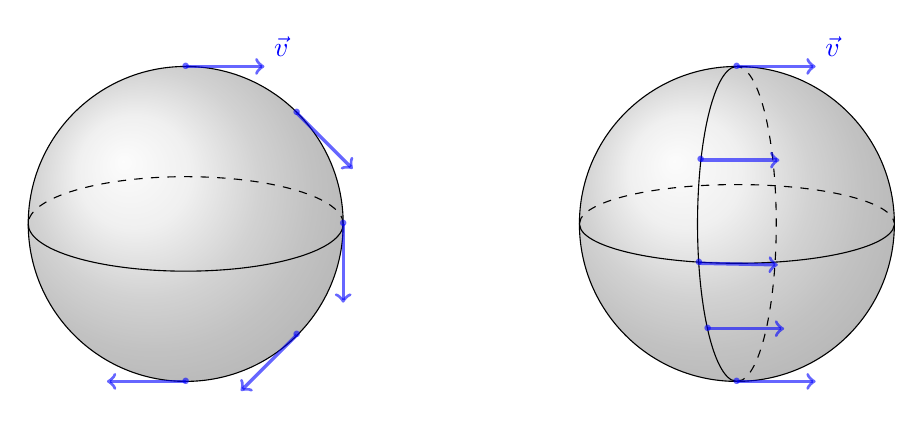
\begin{tikzpicture}[scale = 1]
                            \shade[ball color = gray!40, opacity = 0.4] (0,0) circle (2cm);
                            \draw (0,0) circle (2cm);
                            \draw (-2,0) arc (180:360:2 and 0.6);
                            \draw[dashed] (2,0) arc (0:180:2 and 0.6);
                            \draw[->, very thick, blue, opacity = 0.6] (0,2) node[scale = 0.6]{$\bullet$} -- (1, 2);
                            \draw[blue] (1, 2) node[above right]{$\vec{v}$};
                            \draw[->, very thick, blue, opacity = 0.6] (1.41,1.41) node[scale = 0.6]{$\bullet$} -- (2.12, 0.7);
                            \draw[->, very thick, blue, opacity = 0.6] (2,0) node[scale = 0.6]{$\bullet$} -- (2, -1);
                            \draw[->, very thick, blue, opacity = 0.6] (1.41,-1.41) node[scale = 0.6]{$\bullet$} -- (0.7, - 2.12);
                            \draw[->, very thick, blue, opacity = 0.6] (0,-2) node[scale = 0.6]{$\bullet$} -- (-1, -2);
                            
                            \shade[ball color = gray!40, opacity = 0.4] (7,0) circle (2cm);
                            \draw (7,0) circle (2cm);
                            \draw[dashed] plot [domain =-2:2, samples = 200] (\x+7, {(0.5*sqrt(1-((\x)/2)^2)});
                            \draw plot [domain =-2:2, samples = 200] (\x+7, {(-0.5*sqrt(1-((\x)/2)^2)});
                            \draw plot [domain =-2:2, samples = 200] ({(-0.5*sqrt(1-((\x)/2)^2)+7},\x);
                            \draw[dashed] plot [domain =-2:2, samples = 200] ( {(0.5*sqrt(1-((\x)/2)^2)+7},\x);
                            \draw[->, very thick, blue, opacity = 0.6] (7,2) node[scale = 0.6]{$\bullet$} -- (8, 2);
                            \draw[blue] (8, 2) node[above right]{$\vec{v}$};
                            \draw[->, very thick, blue, opacity = 0.6] (6.54,0.81) node[scale = 0.6]{$\bullet$} -- (7.54, 0.81);
                            \draw[->, very thick, blue, opacity = 0.6] (6.52,-0.5) node[scale = 0.6]{$\bullet$} -- (7.52, -0.52);
                            \draw[->, very thick, blue, opacity = 0.6] (6.63,-1.33) node[scale = 0.6]{$\bullet$} -- (7.6, -1.33);
                            \draw[->, very thick, blue, opacity = 0.6] (7,-2) node[scale = 0.6]{$\bullet$} -- (8, -2);
                        \end{tikzpicture}
                        \caption{Transport parallèle d'un vecteur tangent à la sphère suivant deux chemins différents}
                        \label{fig:my_label}
                    \end{figure}
                \end{exmp}
                
                Comment faire pour que le transport parallèle ne dépende pas du chemin en question? Prenons des chemins infinitésimaux.
                %schéma eliott
                
                Le transport parallèle du vecteur $V$ en $P$ le long du chemin infinitésimale donne un vecteur $\widetilde{V}$ en $P$. Pour cela, on doit faire une intégration infinitésimale de l'équation \ref{eq:transportv}.
                
                \begin{prop}\begin{leftbar}
                    La solution de l'équation
                    \begin{equation}
                        \frac{dV^a}{d\lambda} + \Gamma^a_{\mu b}\frac{dx^\mu}{d\lambda} = 0
                    \end{equation}
                    est 
                    \begin{equation}
                        V(\lambda) = \left[P(0)e^{-\int_0^\lambda d\widetilde{\lambda}V(\widetilde{\lambda})}\right]V(0)
                    \end{equation}
                    où les \textit{produit ordonné} $P$ est définit comme
                    \begin{equation}
                        P\left(V(\lambda_1)V(\lambda_2)\right) ~\hat{=}~ V(\lambda_1) V(\lambda_2)\theta(\lambda_1-\lambda_2)+V(\lambda_2) V(\lambda_1)\theta(\lambda_2-\lambda_1).
                    \end{equation}
                \end{leftbar}\end{prop}
                
                \begin{proof}
                    Cette équation peut être réécrite comme
                    \begin{equation}
                        \frac{dV}{d\lambda} = -A(\lambda)V
                    \end{equation}
                    avec $A(\lambda) = \Gamma_\mu \frac{dx^\mu}{d\lambda}$. La forme intégrale de cette équation est 
                    \begin{equation}
                        V(\lambda) = V(0) - \int_0^\lambda d\lambda_1 A(\lambda_1)V(\lambda_1)
                    \end{equation}
                    C'est une équation équivalente. On peut trouver une solution formelle à cette équation en utilisant une méthode perturbative. En substituant cette équation dans elle-même, nous obtenons
                    \begin{equation}
                        V(\lambda) = V(0) - \int_0^\lambda d\lambda_1 A(\lambda_1)V(0)+\int_0^\lambda d\lambda_1\int_0^{\lambda_1}d\lambda_2A(\lambda_1)A(\lambda_2)V(\lambda_2).
                    \end{equation}
                    
                    On peut répéter ce processus une infinité de fois pour trouver
                    \begin{equation}
                        V(\lambda) = V(0) + \sum_{n=1}^\infty\frac{(-1)^n}{n!}\int_{0\leq\lambda_n\leq\lambda_{n-1}}d\lambda_1\dots d\lambda_n A(\lambda_1)\dots A(\lambda_n)V(\lambda_n).
                    \end{equation}
        
                    Les variables d'intégration $\lambda_1,\dots,\lambda_n$ satisfont $\lambda\geq\lambda_1\geq\dots\geq\lambda_n\geq0$ ce qui permet dé réécrire cette équation avec une seule intégral et des fonction $\theta$ de de Heaviside.
                    
                    \begin{align}
                        V(\lambda) &= V(0) + \sum_{n=1}^\infty\frac{(-1)^n}{n!}\int_{0\leq\lambda_n\leq\lambda_{n-1}}d\lambda_1\dots d\lambda_n V(\lambda_1)\dots V(\lambda_n)\theta(\lambda_1-\lambda_2)\dots\theta(\lambda_{n-1}-\lambda_n) \\
                        &= V(0) + \sum_{n=1}^\infty\frac{(-1)^n}{n!}\int_{0\leq\lambda_n\leq\lambda_{n-1}}d\lambda_1\dots d\lambda_n P\left(V(\lambda_1)\dots V(\lambda_n)\right)\\
                        &= \left[P(0)e^{-\int_0^\lambda d\widetilde{\lambda}V(\widetilde{\lambda})}\right]V(0)
                    \end{align}
                \end{proof}
                
                \begin{rmk}
                    La méthode perturbative utilise dans le démonstration précédente est très utilisée en QFT. Dans ce cas, on utilise le produit chronologique $T$ (pour "time ordered") au lieu de produit ordonnée $P$ (pour "path ordered") car les variables d'intégration sont les variables temporelles.
                \end{rmk}
                
                Dans notre cas, comme il s'agit de chemins infinitésimaux, on peut se limiter à un développement à l'ordre quadratique. On peut montré que développer au premier ordre n'est pas suffisant.
                \begin{equation}
                        V(\lambda_2) = V(0) - \int_1^\lambda d\lambda_2 A(\lambda')V(\lambda_1)+\frac{1}{2}\int_{\lambda_1}^{\lambda_2} d\lambda'\int_{\lambda_1}^{\lambda'}d\lambda''A(\lambda')A(\lambda')V(\lambda_1).
                    \end{equation}
                Notons $V(\lambda_1)\equiv V_1$ et $V(\lambda_2)\equiv V_2$. Dans ce cas, en utilisant la forme explicite de $A$, on trouve que 
                \begin{equation}
                    V_2^\mu = V_1^\mu - \oint \Gamma^\mu_{\nu\rho} dx^\nu V_1^\rho+\frac{1}{2}\int_{\lambda_1}^{\lambda_2} d\lambda'\int_{\lambda_1}^{\lambda'}d\lambda''A^\mu_{~\sigma}(\lambda')A^\sigma_{~\kappa}(\lambda'')V_1^\kappa.
                \end{equation}
                En notation matricielle, 
                \begin{equation}
                    V_2 = V_1 - \oint \Gamma V_1+\frac{1}{2}\int_{\lambda_1}^{\lambda_2} d\lambda'\int_{\lambda_1}^{\lambda'}d\lambda''\Gamma_\rho(\lambda_1)\Gamma_\xi(\lambda'')\frac{dx^\rho}{d\lambda'}\frac{dx^\xi}{d\lambda''} V_1.
                \end{equation}
                Par le théorème de Stokes,
                \begin{equation}
                     \oint \Gamma V_1 = \int_\Sigma d\gamma V_1
                \end{equation}
                avec $\Sigma$ telle que $\p\mathscr{C}$. Le terme $\Gamma_\rho(\lambda_1)\Gamma_\xi(\lambda'')$ peut s'exprimer comme $\eval{\Gamma_\rho\Gamma_\xi}_\mathscr{C}$ plus des corrections qui diminuent avec la taille du contour. On peut donc les négliger.
                \begin{equation}
                    V_2 = V_1-\int_\Sigma v_1 d\Gamma + \Gamma_\rho\Gamma_\xi \int_{\lambda_1}^{\lambda_2}d\lambda'\frac{dx^\rho}{d\lambda'}(\x^\xi(\lambda')-x^\xi(\lambda_1))V_1+\dots
                \end{equation}
                Or, si l'on intègre par partie,
                \begin{equation}
                    \int x^\xi dx^\rho = -\oint x^\rho dx^\xi = \int_\Sigma dx^\xi\wedge dx^\rho = \int_\Sigma d(x^\xi dx^\rho) = \text{aire de }\Sigma
                \end{equation}
                car le chemin est fermé. Finalement, on peut écrire $V_2$ comme
                \begin{align}
                    V_2 &= V_1-\int_\Sigma V_1 d\Gamma + \Gamma_\rho\Gamma_\xi\oint V_1x^\xi dx^\rho +\dots\\
                    &= \left( \mathbb{1}-\int_\Sigma d\Gamma + \Gamma_\rho\Gamma_\xi \int dx^\xi\wedge dx^\rho+\dots \right)V_1 \\
                    &= \left( \mathbb{1}-\int_\Sigma d\Gamma+\Gamma\wedge\Gamma \right)V_1 \\
                    &= \left( \mathbb{1}-\int_\Sigma \mathscr{R} \right)V_1
                \end{align}
                On a obtenu une formule complètement géométrique qui fait apparaître $\mathscr{R}$. On voit que le courbure est le générateur infinitésimale du transport parallèle le long d'un contour fermé.\\
                
                Le résultat s'écrit de manière très élégante :
                \begin{equation}
                    \widetilde{V}^a(P) = \int_\Sigma \mathscr{R}^a_{~b} V^b(P)
                \end{equation}
                où $\Sigma = \p\mathscr{C}$. C'est une version généralisée du théorème de Stokes.\\
                
                Par conséquent, si $\mathscr{R} = 0$, $V_2 = V_1$ le long d'un transport parallèle le long d'un contour fermé. Ceci implique que $V_2 = V_1$ le long d'un contour fermé de taille finie. En effet, on peut toujours décomposé un contour fermé de taille finie en une somme de contours fermé de taille infinitésimale.\\
                
                Ceci montre que si $\mathscr{R} = 0$ et $\{e_a(P)\}$ est une base de $\F_P$, alors on peut définir une base $\{e_a(Q)\}$ pour tout $Q\in\M$ en transportant parallèlement les vecteur de $\{e_a(P)\}$ en $Q$ le long d'un contour joignant $P$ à $Q$. Dans une telle base, $\nabla_{e_a} = 0$ et donc $\Gamma = 0$.\\
                
                Dans le cadre de la relativité générale, ceci implique que si $R_{\mu\nu\rho\sigma} = 0$, alors il existe un référentiel dans lequel $g = \eta$ partout : on a affaire à un espace plat.\\
            
                Nous allons maintenant nous intéresser à deux identité très importants : les identités de Bianchi.
                
                \begin{prop}[première identité de Bianchi]\begin{leftbar}
                    Soit $T$ le tenseur de torsion et $\{e_a\}$ une base de $T_P\M$. Dans ce cas,
                    \begin{equation}
                        dT = \mathscr{R} \wedge e - \Gamma\wedge T
                    \end{equation}
                \end{leftbar}\end{prop}
                
                \begin{proof}
                    Il suffit de partir de la définition $T = de+\Gamma\wedge e$.
                    \begin{align}
                        dT &= d\Gamma\wedge e - \Gamma \wedge de\\
                        &= (\mathscr{R}-\Gamma\wedge\Gamma)\wedge e-\Gamma\wedge(T-\Gamma\wedge e)\\
                        &= \mathscr{R} \wedge e - \Gamma\wedge T
                    \end{align}
                \end{proof}
                
                \begin{prop}[deuxième identité de Bianchi]\begin{leftbar}
                    Soit $T$ le tenseur de torsion et $\{e_a\}$ une base de $T_P\M$. Dans ce cas,
                    \begin{equation}
                        d\mathscr{R} = \mathscr{R} \wedge \Gamma - \Gamma\wedge \mathscr{R}
                    \end{equation}
                \end{leftbar}\end{prop}
                
                \begin{proof}
                    Il suffit de partir de la définition $\mathscr{R} = d\Gamma+\Gamma\wedge\Gamma$.
                    \begin{align}
                        d\mathscr{R} &= d\Gamma\wedge\Gamma-\Gamma\wedge d\Gamma\\
                        &= (\mathscr{R}-\Gamma\wedge\Gamma)\wedge\Gamma - \Gamma\wedge(\mathscr{R}-\Gamma\wedge\Gamma)\\
                        &= \mathscr{R} \wedge \Gamma - \Gamma\wedge \mathscr{R}
                    \end{align}
                \end{proof}
                
                Dans le cas où $T = 0$, la première identité de Bianchi donne
                \begin{align}
                    0 &= \mathscr{R}\wedge e\\
                    &= \mathscr{R}^a_{~d}\wedge e^d\\
                    &= \mathscr{R}^a_{~dbc}\wedge e^b\wedge e^c\wedge e^d \\
                    &= \mathscr{R}^a_{~[bcd]}\\
                    &= \mathscr{R}^a_{~bcd}+\mathscr{R}^a_{~dbc}+\mathscr{R}^a_{~cdb}\label{eq:idbianchi}
                \end{align}
                
            \subsection{Cas de la connexion de Levi-Civita}
                        
                Dans cette section nous allons particulariser les résultats plus généraux qui ont été étudiés avant au cas de la relativité générale. Nous supposons donc dès à présent que nous avons la métrique $g$ et la connexion de Levi-Civita. \\
                
                Dans ce cas-ci, les indices de fibre $a$ et $b$ et les indices d'espace tangent $\mu$ et $\nu$ sont de même nature. Ceci implique que $\mathscr{R}^a_{~b\mu\nu}$ est un tenseur.
                \begin{equation*}
                    \mathscr{R}^\rho_{~\sigma\mu\nu}\to R^\rho_{~\sigma\mu\nu}
                \end{equation*}
                
                \begin{defn}
                    Le tenseur de composantes 
                    \begin{equation}
                        \mathscr{R}^\rho_{~\sigma\mu\nu} = \p_\rho\Gamma^\mu_{\sigma \nu}-\p_\sigma\Gamma^\mu_{\rho\nu} + \Gamma^\mu_{\rho \theta}\Gamma^\theta_{\sigma\nu}-\Gamma^\mu_{\sigma \theta}\Gamma^\theta_{\rho\nu}
                    \end{equation}
                    est de type $(3,1)$ est appelé $\textit{tenseur de Riemann}$.
                \end{defn}
                
                \begin{prop}\begin{leftbar}
                    Le tenseur de Riemann a les propriétés suivantes:
                    \begin{enumerate}[label = \textit{\roman*)}]
                        \item anti-symétrie par rapport aux deux premiers indices :
                        \begin{equation}
                            R_{\mu\nu\sigma\rho} = -R_{\nu\mu\sigma\rho}
                        \end{equation}
                        \item symétrie par rapport aux couples d'indices successifs :
                        \begin{equation}
                            R_{\mu\nu\sigma\rho} = R_{\sigma\rho\mu\nu}
                        \end{equation}
                        \item anti-symétrie par rapport aux deux derniers indices :
                        \begin{equation}
                            R_{\mu\nu\sigma\rho} = -R_{\nu\mu\sigma\rho}
                        \end{equation}
                        \item \textit{première identité de Bianchi} :
                        \begin{equation}
                        R_{\mu\nu\sigma\rho}+R_{\mu\rho\nu\sigma}+R_{\mu\sigma\rho\nu} = 0
                        \end{equation}
                        Nous faisons une permutation cyclique des trois dernier indices.
                        \item \textit{deuxième identité de Bianchi} :
                        \begin{equation}
                            \nabla_\mu R_{\nu\rho\sigma\theta} + \nabla_\theta R_{\nu\rho\mu\sigma}+\nabla_\sigma R_{\nu\rho\theta\mu} = 0
                        \end{equation}
                        Nous faisons une permutation cyclique de l'indice de $\nabla$ et des deux dernier indices de $R$.
                    \end{enumerate}
                \end{leftbar}\end{prop}
                
                \begin{proof}${}$\\
                    \begin{enumerate}[label = \textit{\roman*)}]
                        \item Voir début du cours.
                        \item Voir début du cours. Notons que ce résultat n'est vrai que pour la connexion de Levi-Civita.
                        \item Direct d'après les deux premières propriétés.
                        \item Nous avons montré que la connexion de Levi-Civita est de torsion nulle. Ceci implique que la formule \ref{eq:idbianchi} est valable.
                        \item On sait que, pour $T\in\M$, il existe une base localement plate $(x^\alpha_P)$ dans laquelle $\Gamma = 0$ (montré dans la section précédente). Dans cette base, la deuxième identité de Bianchi prend la forme
                        \begin{equation}
                            dR = 0
                        \end{equation}
                        ou encore
                        \begin{align}
                            dR^\alpha_{~\beta} &= \frac{1}{2} \p_\varepsilon R^\alpha_{~\beta\gamma\delta}~dx^\varepsilon\wedge dx^\gamma\wedge dx^\delta &= 0\\
                            \Leftrightarrow\qquad \p_\varepsilon R^\alpha_{~\beta\gamma\delta} + \p_\gamma R^\alpha_{~\beta\delta\epsilon} + \p_\delta R^\alpha_{~\beta\gamma\varepsilon}
                        \end{align}
                        Il suffit juste d'utiliser le fait que $\nabla_\mu = \p_\mu$ dans des coordonnées locales plates et on trouve bien la relation voulue. Nous avons montré que le résultat étant vrai dans un système de coordonnée en particulier. Comme $R$ est un tenseur, cela reste vrai dans tout les autre système de coordonnées.
                    \end{enumerate}
                \end{proof}
                
                \begin{prop}\begin{leftbar}
                    Le nombre de composantes indépendantes du tenseur de Riemann est
                    \begin{equation}
                        \frac{1}{12}D^2(D^2-1).
                    \end{equation}
                    En particulier pour $n=4$, les tenseur de Riemann possède $20$ composantes indépendantes.
                \end{leftbar}\end{prop}
                
                \begin{proof}
                    Le nombre de composantes indépendantes d'un tenseur de rang $4$ qui ets symétrique sous l'échange des couples d'indices successifs est 
                    \begin{equation}
                        \frac{1}{2}D(D-1)\frac{1}{2}D(D-1)
                    \end{equation}
                    Si de plus ce tenseurs est anti-symétrique sous l'échange des premiers indices, alors ce nombre de devient
                    \begin{equation}
                        \frac{1}{2}\frac{1}{2}D(D-1)\left( \frac{1}{2}D(D-1)1+ \right).
                    \end{equation}
                    Pour tenir compte de l'identité de Bianchi, on observe que le tenseur
                    \begin{equation}
                        t_{\mu\nu\sigma\rho} = R_{\mu\nu\sigma\rho}+R_{\mu\rho\nu\sigma}+R_{\mu\sigma\rho\nu}
                    \end{equation}
                    est complètement anti-symétrique. Le nombre de composantes indépendantes final est donc 
                    \begin{equation}
                        \frac{1}{2}\frac{1}{2}D(D-1)\left( \frac{1}{2}D(D-1)1+ \right)  -\frac{D(D-1)(D-2)(D-3)}{4!}.
                    \end{equation}
                \end{proof}
                
                Pour rappel, le nombre d'invariantes de courbure est le nombre de quantités scalaires indépendantes que l'on peut construire avec $R$ et $g$.
                
\chapter{Équation d'Einstein}

    
        
    \section{Tenseur de Ricci et tenseur d'Einstein}
        
        \begin{defn}
            On définit le \textit{tenseur de Ricci} comme étant le tenseur de composantes
            \begin{equation}
                R_{\mu\nu} ~\hat{=}~ R^\rho_{~\mu\rho\nu}.
            \end{equation}
        \end{defn}
        
        \begin{prop}\begin{leftbar}
            Le tenseur de Ricci a les propriétés suivantes :
            \begin{enumerate}[label = \textit{\roman*)}]
                \item c'est un tenseur symétrique : $R_{\mu\nu} = R_{\nu\mu}$
                \item c'est la seule contraction non-nulle des composantes du tenseur de Riemann
            \end{enumerate}
        \end{leftbar}\end{prop}
        
        \begin{proof}${}$
            \begin{enumerate}[label = \textit{\roman*)}]
                \item Cette propriété se déduit directement de la première identité de Bianchi.
                \begin{align}
                    R_{\mu\nu\mu\rho}+R_{\mu\rho\nu\mu}+\underbrace{R_{\mu\mu\rho\nu}}_{0} &= 0\\
                    \Leftrightarrow\qquad R_{\nu\rho} - R_{\rho\nu} &= 0
                \end{align}
                \item En utilisant les propriétés de symétrie et d'anti-symétrie des indices de $R$, on voit que la contraction des indices $1-2$,$3-4$,$1-4$ et $2-3$ est nulle. Et par symétrie, la contraction des indices $2-4$ est la même que le tenseur de Ricci.
            \end{enumerate}
        \end{proof}
        
        Notons que le tenseur de Ricci contient de l'information sur la géométrie de l'espace-temps mais tout de même moins que le tenseur de Riemann.
        
         \begin{defn}
            Le \textit{scalaire de Ricci} est définit comme
            \begin{equation}
                R ~\hat{=}~ R^\mu_{~\mu}.
            \end{equation}
        \end{defn}
        
        \begin{defn}
            Le \textit{tenseur d'Einstein} est définit comme
            \begin{equation}
                G_{\mu\nu} ~\hat{=}~ R_{\mu\nu}-\frac{1}{2}Rg_{\mu\nu}.
            \end{equation}
        \end{defn}
        
        \begin{prop}\begin{leftbar}
            Le tenseur d'Einstein a les propriétés suivantes :
            \begin{enumerate}[label = \textit{\roman*)}]
                \item c'est un tenseur symétrique : $G_{\mu\nu} = G_{\nu\mu}$
                \item on a la relation :
                \begin{equation}
                    \nabla_\mu G^{\mu\nu} = 0
                \end{equation}
            \end{enumerate}
        \end{leftbar}\end{prop}
        
        \begin{proof}${}$
            \begin{enumerate}[label = \textit{\roman*)}]
                \item Direct par la symétrie de $g$ et de $R$.
                \item D'après la deuxième identité de Bianchi, 
                \begin{align}
                    0& =\nabla_\mu R_{\nu\rho\sigma\theta} + \nabla_\theta R^\nu_{~\theta\rho\mu}+\nabla_\sigma R_{\nu\rho\theta\mu} \\
                    &= \nabla_\mu R_{\theta\rho}+\nabla_\mu R^\nu_{~\theta\rho\mu} - \nabla_\rho R_{\theta\mu} \\
                    &= \nabla_\mu R + g^{\theta\rho} \nabla_\nu R^\nu_{~\theta\rho\mu} - \nabla_\rho R_{\rho\mu} 
                \end{align}
                \begin{align}
                    g^{\theta\rho} \nabla_\nu R^\nu_{~\theta\rho\mu} &= \nabla_\nu (g^{\theta\rho}R^\nu_{~\theta\rho\mu}) \\
                    &= \nabla^\nu (g^{\theta\rho}R_{~\nu\theta\rho\mu})\\
                    &= -\nabla^\nu R_{\nu\mu}
                \end{align}
                Nous obtenons 
                \begin{align}
                    0 &= \nabla_\mu R -\nabla^\nu R_{\nu\mu} - \nabla_\rho R_{\rho\mu}\\
                    &= \p_\mu R -2\nabla^\rho R_{\rho\mu}
                \end{align}
                car la dérivée covariante d'un scalaire revient à faire la dérivée normale. D'autre part, si on développe l'expression de $G_{\mu\nu}$,
                \begin{align}
                    \nabla^\mu G_{\mu\nu} &= \nabla^\mu \left(R_{\mu\nu}-\frac{1}{2}Rg_{\mu\nu}\right)\\
                    &= \nabla^\mu R_{\mu\nu}-\frac{1}{2}\nabla^\mu Rg_{\mu\nu}-\frac{1}{2}R \underbrace{\nabla^\mu g_{\mu\nu}}_{0}\\
                    &= \nabla^\mu R_{\mu\nu} -\frac{1}{2}g_{\mu\nu}\p^\mu R \\
                    &= \nabla^\mu R_{\mu\nu} -\frac{1}{2}\p_\nu R 
                \end{align}
                ce qui fait bien $0$ par ce qui précède.
            \end{enumerate}
        \end{proof}
        
        Ces propriétés sont des versions contractées des identités de Bianchi.
                
    \section{Équations de champ}
    
        \subsection{Tenseur énergie-impulsion}
        
            On cherche une équation de la forme
            \begin{equation*}
                \textbf{source du champ de gravitation} = \textbf{champ de gravitation}
            \end{equation*}
            qui relie un terme de source à la géométrie de l'espace-temps. En mécanique newtonienne, la source du champ de gravitation est la masse. Dans notre cas, on cherche un tenseur pour trouver une équation tensorielle. En relativité restreinte, il y a l'équivalence masse-énergie, la masse étant la composante $00$ du tenseur énergie-impulsion $T^{\mu\nu}$. Ce tenseur caractérise le contenu en énergie et en impulsion de la matière et du champ électro-magnétique, il a deux propriétés fondamentales : il est symétrique et conservé : $\p_\alpha T^{\alpha\beta} = 0$. En présence de gravité, cette l'équation de conservation devient
            \begin{equation}
                \nabla_\mu T^{\mu\nu} = 0.
            \end{equation}
            Cette équation sera satisfaite dès que les équations du mouvement pour la matière ou le rayonnement (encore à déterminer) sont satisfaites.\\
            
            En relativité générale, il n'y a pas de notion d'invariance par translation et donc pas de conservation de l'énergie. Cependant, l'équation que l'on vient de voir est bien satisfaite, mais elle ne permet pas la construction d'une quantité $E$ qui est conservée dans tous les référentiels. La différence fondamentale entre le champ de gravitation et les autres champs est qu'il n'a pas de tenseur énergie-impulsion qui lui est associé. Supposons que ce soit le cas: par le principe d'équivalence, il n'y a pas de gravité dans des coordonnées localement plates et donc le tenseur énergie-impulsion du champ de gravitation serait nul dans cette base de coordonnées. Ce qui entraîne donc qu'il serait également nul dans tous les autres référentiels.
            
            \begin{exmp}
                Pour le champ électro-magnétique, 
                \begin{equation}
                    T^{\mu\nu} = F^{\mu\rho}F^{\nu}_{~\rho}-\frac{1}{4}F^{\rho\sigma}F_{\rho\sigma}g^{\mu\nu}.
                \end{equation}
            \end{exmp}
            
            \begin{exmp}
                Pour une particule ponctuelle de masse $m$, le tenseur énergie-impulsion est
                \begin{equation}
                    T^{\mu\nu}(x) = m\int U^\mu(\tau)U^\nu(\tau)\frac{\delta\left(x-\hat{x}(\tau)\right)}{\sqrt{\abs{\det(g)}}} ~d\tau
                \end{equation}
                où $\hat{x}(\tau)$ est la ligne d'univers de la particule. En relativité restreinte, $\det(g) = \det(\eta) = 1$ et
                \begin{equation}
                    U^\mu = \left( \frac{dx^0}{d\tau},\frac{dx^1}{d\tau} \right) = \gamma(1,\vv{v}).
                \end{equation}
                donc la composante $T^{00}$ est
                \begin{align}
                    T^{00}(t\vv{x}) &= m\int\gamma^2 \delta(t-\hat{x}^0(\tau))\delta(\vv{x}-\hat{\vv{x}}(\tau)) \frac{dt}{\gamma} \\
                    &= m\gamma \delta(\vv{x}-\hat{\vv{x}}(\tau))
                \end{align}
                c'est-à-dire la densité d'énergie au point $\vv{x}$.
                Les composantes $T^{0i}$ sont
                \begin{align}
                    T^{0i}(t,\vv{x}) &= m\int\gamma^2 v^i\delta(t-\hat{x}^0(\tau))\delta(\vv{x}-\hat{\vv{x}}(\tau)) \frac{dt}{\gamma} \\
                    &= m\gamma v^i \delta(\vv{x}-\hat{\vv{x}}(\tau))
                \end{align}
                c'est-à-dire la densité d'impulsion au point $\vv{x}$.\\
                
                En présence de gravité, $\det(g)\neq 1$ donc $\delta(\vv{x}-\hat{\vv{x}}(\tau))$ devient
                \begin{equation} \frac{\delta(\vv{x}-\hat{\vv{x}}(\tau))}{\sqrt{\abs{\det(g)}}}.
                \end{equation}
                Montrons que cette fonction se transforme bien comme un scalaire. Si $x'$ est un second système de coordonnées, nous avons d'une part
                \begin{equation}
                    \delta(x'(x)) = \frac{\delta(x-x_0)}{\abs{\det\left( \pdv{x'}{x} \right)}}
                \end{equation}
                si $x = x_0\Leftrightarrow x' = 0$ et d'autre part
                \begin{equation}
                    g'_{\mu\nu}(x) = \pdv{x^\rho}{x'^\mu}\pdv{x^\sigma}{x'^\nu} g_{\rho\sigma}(x)
                \end{equation}
                donc
                \begin{equation}
                    \sqrt{\abs{\det(g')}} = \sqrt{\abs{\det\left( \pdv{x}{x'}\right)^2 \det(g)}} = \abs{\det\left(\pdv{x}{x'}\right)} \sqrt{\abs{\det(g)}}.
                \end{equation}
                On retrouve bien
                \begin{equation}
                    \frac{\delta(x'(x))}{\sqrt{\abs{\det(g)}}} = \frac{\delta(x-x_0)}{\sqrt{\abs{\det(g)}}}\frac{1}{\abs{\det\left( \pdv{x'}{x}\right)\det\left( \pdv{x}{x'}\right)}} = \frac{\delta(x-x_0)}{\sqrt{\abs{\det(g)}}}.
                \end{equation}
                Donc les $T^{\mu\nu}$ sont bien les composantes d'un tenseur.
            \end{exmp}
            
            \begin{exmp}
                Les fluides parfaits sont caractérisés par la densité d'énergie $\rho$ et la pression $p$. Si le fluide est au repos, le tenseur énergie-impulsion prend la forme 
                \begin{equation}
                    T^{\alpha\beta} = 
                    \begin{bmatrix}
                        \rho & 0 & 0 & 0 \\
                        0 & p & 0 & 0 \\
                        0 & 0 & p & 0 \\
                        0 & 0 & 0 & p
                    \end{bmatrix}
                \end{equation}
                Si le fluide est caractérisé par un champ de vitesse $U^\alpha(x)$, le tenseur énergie-impulsion doit être de la forme
                \begin{equation}
                    T^{\alpha\beta} = A U^\alpha U^\beta + B \eta^{\alpha\beta}
                \end{equation}
                avec $A,B\in\mathbb{R}$. Si $U^\alpha(x) = 0$, le fluide est au repos et on a donc les conditions
                \begin{subequations}
                    \begin{empheq}[left=\empheqlbrace]{align}
                        T^{00} &= A-B = \rho\\
                        T^{ii} &= B = p
                    \end{empheq}
                \end{subequations}
                ce qui détermine $A$ et $B$. On obtient
                \begin{equation}
                    T^{\alpha\beta} = (\rho+p)U^\alpha U^\beta + p \eta^{\alpha\beta}.
                \end{equation}
                Cette formule est valable uniquement lorsqu'il n'y a pas de champ de gravitation. Quand il y a un champ de gravitation, l'expression précédente devient
                \begin{equation}
                    T^{\alpha\beta} = (\rho+p)U^\alpha U^\beta + p g^{\alpha\beta}.
                \end{equation}
                Si l'on modélise le rayonnement, on doit avoir $Tr(T) = 0$. Or, $Tr(T) = T^\mu_{~\mu} = -\rho-p+4p$ donc on retrouve la relation
                \begin{equation}
                    \rho = 3p
                \end{equation}
                pour le rayonnement. Cet exemple illustre une méthode pour modéliser processus/champs. Ici le rayonnement.
            \end{exmp}
        
        \subsection{Conditions sur l'énergie}
        
            On peut imposer un grands nombre de conditions sur l'énergie. Nous en détaillerons trois des plus courantes.
            
            \begin{defn}
                \textit{Condition faible} : un observateur local mesure toujours une densité d'énergie positive.
            \end{defn}
            
            Si un observateur est au repos, cette condition impose que $T^{00}\geq 0$. De manière générale, si $U^\mu$ est la quadri-vitesse de l'observateur, cela revient à imposer $T_{\mu\nu}U^\mu U^\nu \geq 0$ pour tout quadri-vecteur $U$ de genre temps. La condition faible sur l'énergie est donc équivalent à imposer 
            \begin{equation}
                T_{\mu\nu}U^\mu U^\nu \geq 0\qquad \forall U^2\leq 0.
            \end{equation}
            
            \begin{rmk}
                Notons que la condition est valable uniquement pour les observateur dont les quadri-vitesse sont de genre temps : $U^2<0$. Cependant, tout vecteur de genre lumière peut être obtenu comme la limite de vecteurs de genre temps. Ce résultat reste donc valable pour $U^2\leq0$ comme indiqué.
            \end{rmk}
            
            \begin{exmp}
                Vérifions que c'est valable pour le champ électromagnétique.
                \comp
            \end{exmp}
            
            \begin{exmp}
                Pour les fluides parfaits, c'est vrai uniquement si $\rho\geq -p$. En effet,
                \comp
            \end{exmp}
            
            \begin{defn}
                \textit{Condition dominante} : en plus de la condition faible, tout observateur voit un flux d'énergie décrit par un vecteur de genre temps.
            \end{defn}
            
            Ceci signifie que l'énergie "se déplace" moins vite que la lumière. Si un observateur est caractérisé par une quadri-vitesse $U^\mu$, le flux d'énergie qu'il observe est $T^{\mu\nu}U_\nu$. La condition dominante impose donc que ce quadri-vecteur soit de genre temps pour tout $U$ de genre temps. C'est-à-dire
            \begin{equation}
                (T^{\mu\nu}U_\nu)^2\leq0 \qquad\forall U^2\leq0
            \end{equation}
            en plus de la condition faible.
            
            \begin{exmp}
                Vérifions cela pour le champ électromagnétique.
                \comp
            \end{exmp}
            
            \begin{exmp}
                Pour les fluides parfaits, cette condition est respectée si $\rho\geq\abs{p}$. En effet,
                \comp
            \end{exmp}
            
            \begin{defn}
                \textit{Condition forte} : on impose
                \begin{equation}
                    T_{\mu\nu}U^\mu U^\nu \leq \frac{T}{2} U^2\qquad \forall U^2\leq0
                \end{equation}
                où $T = = T^\mu_{~\mu}$.
            \end{defn}
        
            Cette condition traduit le fait que la force de gravitation est attractive. Elle est utile pour certains calcul mais elle n'est pas respectée dans le nature (par exemple par l'énergie noire).

        \subsection{Équation d'Einstein}
        
            Pour rappel, on cherche une équation qui lie la géométrie de l'espace-temps à un terme de source. Autrement dit, cette équation doit relier le tenseur de courbure à la généralisation tensorielle de la masse, c'est-à-dire au tenseur énergie-impulsion. Dans un premier temps, désignons le terme qui dépend du tenseur de courbure par un certain tenseur $H_{\mu\nu}$. Cette équation doit être de la forme
            \begin{equation}
                H_{\mu\nu} = \kappa^2 T_{\mu\nu}
            \end{equation}
            où $\kappa^2$ est une certaine constante de proportionnalité. Par propriété du tenseur $T$, $H$ doit satisfaire
            \begin{subequations}
                \begin{empheq}[left=\empheqlbrace]{align}
                    H_{\mu\nu} &= H_{\nu\mu}\\
                    \nabla_\mu H^\mu_{~\nu} &= 0
                \end{empheq}
            \end{subequations}
            Le première équation qu'Einstein a proposée est la suivante:
            \begin{equation}\label{eq:einstein1}
                R_{\mu\nu} = \kappa^2 T_{\mu\nu}
            \end{equation}
            Dans le vide, $T_{\mu\nu} = 0$ et donc cette équation devient
            \begin{equation}
                R_{\mu\nu} = 0.
            \end{equation}
            L'équation \ref{eq:einstein1} induit trop de contrainte sur $R$ et est donc fausse. Cependant, dans le vide, elle donne la même prédiction que la version corrigée de l'équation ce qui qui permit déjà de faire des prédictions qui, après avoir été validées, on mit en avant la théorie de la relativité générale.
            
            \begin{thm}[équation d'Einstein]\begin{leftbar}
                Le tenseur d'Einstein satisfait à l'équation
                \begin{equation}
                    G_{\mu\nu}+\Lambda g_{\mu\nu} = \kappa^2 T_{\mu\nu}.
                \end{equation}
                où la constante $\Lambda>0$ est appellée \textit{constante cosmologique}.
            \end{leftbar}\end{thm}
            Nous verrons que, dans le vide, ces équations permettent bien de retrouver la condition $R = 0$ (en notation matricielle pour le tenseur de Riemann). La constante cosmologique joue un rôle fondamental. Elle est notamment responsable de l'expansion de l'univers.\\
            
            Ces équation sont essentiellement uniques si l'ont impose que le tenseur $G_{\mu\nu}$ du membre de gauche soit construit uniquement à partir de la métrique, ses dérivées premières, ses dérivées secondes et si il satisfait
            \begin{equation}
                \nabla_\mu G^{\mu\nu} = 0.
            \end{equation}
            Si l'ont se trouve en coordonnées localement plates, les dérivées secondes sont les seul termes non triviaux car $g_{\mu\nu}$ et les dérivées premières de $g_{\mu\nu}$ s'annulent.\\
            
            En réalité, ces équations n'ont aucune raison d'être exactes. Ce n'est que les premiers termes dans un développement mettant en jeu des dérivées d'ordre supérieurs. On pourrait donc très bien avoir quelque chose de la forme
            \begin{equation}
                \Lambda g_{\mu\nu} + R_{\mu\nu} - \frac{1}{2}Rg_{\mu\nu} + "R^2" + "\nabla^2R" + "\nabla^4 R"+\dots = \kappa^2 T_{\mu\nu}
            \end{equation}
            où les termes $"\nabla^iR"$ désigne une quantité proportionnelle au dérivée d'ordre $i$ du tenseur de Riemann (et non du scalaire de Ricci). Premièrement, les termes d'ordre $i$ impaire ne sont pas possibles. Il n'est pas possible de contracté un nombre impaire d'indices de manière à former un tenseur d'ordre. Or, l'équation d'Einstein est une relation entre tenseurs d'ordre 2. Deuxièmement, pour que ca soit cohérent au niveau des dimensions, il faut que les termes $"\nabla^i R"$ soit multipliés par quelque chose proportionnel à une longueur $l^i$ car $[\nabla^i]=\frac{1}{L^i}$.
            \begin{equation}
                \Lambda g_{\mu\nu} + R_{\mu\nu} - \frac{1}{2}Rg_{\mu\nu} + "R^2" + l^2"\nabla^2R" + l^2"\nabla^4 R"+\dots = \kappa^2 T_{\mu\nu}
            \end{equation}
            $l$ serait une longueur caractéristique de la théorie. Ça serait une longueur fondamentale dans une théorie microscopique (quantique) de la gravitation. Par exemple la longueur de Planck ou la taille des cordes. Il n'est pas possible de construire une grandeur proportionnelle à une longueur à partir de $G$ et $c$ uniquement, il faut rajouter $\hbar$ par exemple. Si l'on considère des champ de gravitation pour lesquels
            \begin{equation}
                \nabla\sim\frac{1}{L}\ll \frac{1}{l_{\text{Planck}}}
            \end{equation}
            où $L$ est une taille typique à laquelle le champ varie, les termes contenant les dérivées supérieures sont complètement négligeables. Cette égalité est donc remarquable non pas parce qu'elle est exacte à toutes les échelles mais parce qu'elle est universelle : les facteurs de proportionnalité qui serait devant les termes $"\nabla^iR"$ dépendraient du système de coordonnées choisi, mais pas ceux qui sont dans les équations d'Einstein.\\
            
            Discutons d'un problème majeur de cette équation. Comme il faut que
            \begin{equation}
                [\Lambda]=\frac{1}{L^2}
            \end{equation}
            la valeur naturelle de $\Lambda$ est $\Lambda\sim \frac{1}{l_{\text{Planck}}^2}$, ce qui est énorme. Or, on observe $\Lambda_{\text{obs}}\sim\frac{10^{-120}}{l_{\text{Planck}}^2}$. Soit un valeur erronée d'un facteur $10^{120}$ par rapport aux prédictions : c'est la problème de la constante cosmologique. La supersymétrie permet de prédire une valeur de $\Lambda_{\text{obs}}\sim\frac{10^{-60}}{l_{\text{Planck}}^2}$ ce qui est déjà nettement mieux, mais toujours extrêmement éloigné de ce que l'on observe. Ça reste un problème totalement incompris à l'heure actuelle. De plus, cette valeur est absolument nécessaire pour permette à un univers macroscopique (comme le nôtre) d'exister. Une explication possible est de supposer que les lois de la physique ne sont pas uniques et qu'il existent plein solution correspondant à plein d'univers. Les nombre de solution peut être estimé, il est discret et astronomiquement grand. C'est la théorie du multivers. On peut alors se demander pourquoi est-ce que l'on observe cette valeur de $\Lambda$ en particulier alors? Comme la valeur de $\Lambda$ observée est précisément la valeur qui rend possible l'existence d'un univers comme le nôtre (d'après la théorie), c'est en fait la seule valeur que l'on peut observer. C'est le principe anthropique.\\
            
            On sait $\Lambda$ est non-nulle et positive. Mais ca valeur est tellement petite qu'elle joue un rôle complètement négligeable à n'importe quelle échelle plus petite que celle de l'univers (échelle cosmologique). L'ordre de grandeur des échelles à observer pour que la constante cosmologique joue un rôle est 
            \begin{equation}
                l_\Lambda = \frac{1}{\sqrt{\Lambda_{\text{obs}}}}\sim 10^{25}\meter
            \end{equation}
            \begin{align}
                \text{échelle des galaxies} \sim 10^{21}\meter &\to \text{$\Lambda$ complètement négligeable}\\
                \text{échelle des galaxies} \sim 10^{30}\meter &\to \text{$\Lambda$ joue un rôle crucial}
            \end{align}
            
            Plus encore, les seules théories quantiques de la gravitation connues nécessitent $\Lambda<0$.\\
            
            Dans la suite nous travaillerons avec les équations d'Einstein sans constante cosmologique : $\Lambda = 0$.
            \begin{equation}
                R_{\mu\nu}-\frac{1}{2}Rg_{\mu\nu} = \kappa^2 T_{\mu\nu}
            \end{equation}
            
            \begin{defn}
                $R_{\mu\nu} = 0$ est appelée la \textit{condition de Ricci plat}.
            \end{defn}
            
            \begin{prop}\begin{leftbar}
                Dans le vide, l'équation d'Einstein est équivalente à la \textit{condition de Ricci plat}.
            \end{leftbar}\end{prop}
            
            \begin{proof}
                Dans le vide, $T_{\mu\nu}=0$ donc
                \begin{equation}
                    R_{\mu\nu}-\frac{1}{2}Rg_{\mu\nu} = 0.
                \end{equation}
                En prenant la trace de cette équation, on trouve
                \begin{equation}
                    R-2R = 0
                \end{equation}
                et donc
                \begin{equation}
                    R = 0
                \end{equation}
                On retrouve alors la condition de Ricci plat:
                \begin{equation}
                    R_{\mu\nu} = 0
                \end{equation}
            \end{proof}
            Pour rappel, prendre la trace d'un tenseur n'est pas la même chose que sommer les éléments diagonaux de sa représentation matricielle. Pour un tenseur deux fois covariant $A$ de composantes $A_{\mu\nu}$, 
            \begin{equation}
                Tr(A) = A^\mu_{~\mu} = g^{\mu\nu}A_{\nu\mu}.
            \end{equation}
            
            Il faut donc multiplier $A_{\mu\nu}$ par $g^{\nu\mu}$.
            
            \begin{exmp}
                La trace de $g$ est
                \begin{equation}
                    Tr(g) = g^\mu_{~\mu} = g^{\mu\nu}g_{\nu\mu} = \delta^\mu_{~\mu} = 4.
                \end{equation}
            \end{exmp}
            
            
        \subsection{Limite non-relativiste et de champ faible}
        
            Pour rappel, l'équation des géodésique est 
            \begin{align}
                \ddot{x}^\mu + \Gamma^\mu_{\nu\rho}\dot{x}^\nu\dot{x}^\rho = 0
            \end{align}
            avec
            \begin{equation}
                \Gamma^\rho_{\mu\nu} = \frac{1}{2}g^{\rho\sigma}\left( \p_\mu g_{\nu\sigma}+\p_\nu g_{\mu\sigma}-\p_\sigma g_{\mu\nu} \right).
            \end{equation}
            Dans le cas classique, cette équation devient
            \begin{equation}
                \ddot{x}^i + \Gamma^i_{00} = 0
            \end{equation}
            avec
            \begin{equation}
                \Gamma^i_{00} = \frac{1}{2}g^{i\sigma}\left( 2\p_0 g_{0i}-\p_i g_{00} \right) = -\frac{1}{2}\p_i g_{00}.
            \end{equation}
            Ceci nous donne
            \begin{equation}
                \ddot{x}^i = -\Gamma^i_{00} = \frac{1}{2}\p_i g_{00}.
            \end{equation}
            D'autre part, en mécanique classique, $\ddot{x}^i = -\p_i\phi$ où $\phi$ est le potentiel gravitationnel. Donc,
            \begin{equation}
                g_{00}\approx -1-2\phi.
            \end{equation}
            La composante $00$ de l'équation d'Einstein est
            \begin{equation}
                R_{00}+\frac{1}{2}R = \kappa^2 T_{00}
            \end{equation}
            où $T_{00}\equiv\rho$ est la densité d'énergie (et donc de masse car on est dans le cas non-relativiste). D'autre part, si l'on prend la trace de l'équation d'Einstein, on obtient
            \begin{align}
                g^{\nu\mu}R_{\mu\nu} - \frac{1}{2}Rg^{\nu\mu}g_{\mu\nu} &= \kappa^2g^{\nu\mu}T_{\mu\nu}\\
                \Leftrightarrow \qquad R-\frac{4}{2}R &= \kappa^2 T^\mu_{~\mu}\\
                \Leftrightarrow\qquad -R &= \kappa^2 \rho
            \end{align}
            En utilisant cette relation dans la composante $00$ de l'équation d'Einstein on peut exprimer la première composante du tenseur de Riemann en terme la densité d'énergie.
            \begin{equation}
                R_{00} = \frac{1}{2}\kappa^2\rho
            \end{equation}
            Dans notre car, le tenseur de Riemann est 
            \begin{equation}
                R = d\Gamma + \Gamma\wedge\Gamma \approx d\Gamma
            \end{equation}
            car la limite classique ets une limite linéaire et le terme $\Gamma\wedge\Gamma$ n'est pas linéaire. On peut calculer les $R^i_{~j} = R^i_{~0j0}$ à partir de cette approximation comme
            \begin{align}
                R^i_{~0j0} =d\Gamma^i_{~j} = \p_j\Gamma^i_{00}-\underbrace{\p_0\Gamma^i_{j0}}_{\approx 0} = -\frac{1}{2}\p_i\p_j g_{00} = \p_i\p_j \phi.
            \end{align}
            Le terme avec la dérivée temporelle est proportionnel à $\frac{1}{c^2}$ est peut donc être négligé (comme on l'a fait pour la limite non-relativiste de la trajectoire d'une particule test). Ce terme des effets de propagation. Le champ obtenu sera donc instantané. C'est ce à quoi on s'attend pour une théorie classique.\\
            
            Pour finir, la première composante du tenseur de Riemann est obtenue comme
            \begin{equation}
                R_{00} = R^i_{~0i0} = \sum_{i=1}^3 \p_i\p_i \phi = \Delta\phi.
            \end{equation}
            Ceci nous donne l'équation
            \begin{equation}
                \Delta\phi = \kappa^2\rho.
            \end{equation}
            Or, en mécanique newtonienne, le laplacien du potentiel gravitationnel a une valeur bien connue : $\Delta\phi = 8\pi G$. Pour que les équations d'Einstein dans la limite non-relativiste et de champ faible soient cohérentes avec celles de Newton, il faut donc que
            \begin{equation}
                \kappa^2 = 8\pi G.
            \end{equation}
            
            On peut faire une rapide analyse dimensionnelle afin de retrouver les facteurs $c$ pour repasser au SI. Les unités du tenseur énergie impulsion dépendent de la convention utilisée. Dans ce cours nous prendrons $T_{\mu\nu}$ homogène à une densité d'énergie.
            \begin{align}
                [R] &= [R_{\mu\nu}] = \frac{1}{L^2}\\
                [T_{\mu\nu}] &= \frac{ML^2}{T^2}\frac{1}{L^3} = \frac{M}{LT^2}\\
                [G] &= \frac{L^3}{MT^2}
            \end{align}
            Pour l'équation
            \begin{equation}
                R_{\mu\nu}-\frac{1}{2}Rg_{\mu\nu} = c^\alpha 8\pi G T_{\mu\nu}
            \end{equation}
            on a
            \begin{equation}
                \frac{1}{L^2} = \left(\frac{L}{T}\right)^\alpha \frac{L^3}{MT^2}\frac{M}{LT^2}
            \end{equation}
            ce qui donne $\alpha = -4$.
            
            \begin{equation}
                \boxed{R_{\mu\nu}-\frac{1}{2}Rg_{\mu\nu} = \frac{8\pi G}{c^4} T_{\mu\nu}}
            \end{equation}
            
    \section{Équation de déviation géodésique}
        
        Soient deux observateurs situés proches l'un de l'autre dans un champ gravitationnel non-homogène. Si leurs positions n'est pas exactement la même, il arrivera un moment où ces observateurs s'éloigneront l'un de l'autre. Plus le champ de gravitation est fort, plus la distance entre les deux va augmenter rapidement. Ce petite exemple permet de comprendre intuitivement comment est-ce que leur accélérations relatives permet de mesurer le champ de gravitation. L'équation qui relie ces quantités est l'équation de déviation géodésique.\\
        
        \subsection{Cas de Newton}
        
            En mécanique newtonienne, la composante $i$ de l'accélération est donnée par
            \begin{equation}
                \ddot{x}^i = -\p_i\phi.
            \end{equation}
            Les trajectoires possibles sont les solutions de cette équation. On considère la famille de solution $x^i(t,v)$ paramétrée par $v$. De cette manière,
            \begin{equation}
                \pdv[2]{x^i}{t} = -\p_i\phi(x(t,v)).
            \end{equation}
            La séparation entre deux trajectoires voisines est
            \begin{equation}
                \delta x^i = \pdv{x^i}{v}\delta v = N^i \delta v
            \end{equation}
            si l'on définit $N^i~\hat{=}~\pdv{x^i}{v}$. On peut voir que "l'accélération" de cette quantité est
            \begin{align}
                \pdv[2]{N^i}{t} &= \pdv[2]{}{t}\pdv{x^i}{v}\\
                &= \pdv{}{v}\pdv[2]{x^i}{t}\\
                &= -\pdv{}{v}\p_i\phi(x(t,v))\\
                &= -\pdv{x^j}{v}\p_j\p_i\phi\\
                &= -N^j\p_i\p_j\phi
            \end{align}
            L'équation de dérivation géodésique en mécanique newtonienne est donc
            \begin{equation}
                \pdv[2]{N^i}{t} = -N^j\p_i\p_j\phi
            \end{equation}
            
        \subsection{Cas relativiste}
        
            Considérons une famille de géodésiques $x^\mu(\lambda,v)$ paramétrée par $v$ de paramètre affine $\lambda$. De cette manière,
            \begin{equation}
                \ddot{x}^\mu + \Gamma^\mu_{\nu\rho}\dot{x}^\nu\dot{x}^\rho = 0.
            \end{equation}
            La séparation entre deux géodésiques voisines est
            \begin{equation}
                \delta x^\mu = \pdv{x^\mu}{v}\delta v = N^\mu \delta v
            \end{equation}
            si l'on définit $N^\mu~\hat{=}~\pdv{x^\mu}{v}$. Remarquons que $N^\mu$ se transforme comme
            \begin{equation}
                N'^\mu = \pdv{x'^\mu}{v} = \pdv{x'^\mu}{x^\nu}\pdv{x^\nu}{v} = \pdv{x'^\mu}{x^\nu}N^\mu
            \end{equation}
            donc $N^\mu$ sont les composantes d'un vecteur. Commençons par démontrer une relations qui sera utilise.
        
            \begin{prop}\begin{leftbar}
                Si $V^\mu$ sont les composantes d'un vecteur et que $X,Y$ sont deux champs vectoriels alors
                \begin{align}
                    [\nabla_X,\nabla_Y]V^\mu = X^\rho Y^\sigma R^{\mu}_{~\nu\rho\sigma}V^\nu + (\L_X Y)^\sigma\nabla_\sigma V^\mu.
                \end{align}
            \end{leftbar}\end{prop}
            
            \begin{proof}
                Premièrement, nous savons que
                \begin{equation}
                    \nabla_Y V^\mu = Y^\rho(\p_\rho V^\mu+\Gamma^\mu_{\rho\nu}V^\nu).
                \end{equation}
                En prenant la dérivée covariante de cette expression par rapport à $X$, on obtient
                \begin{align}
                    \nabla_X \nabla_Y V^\mu &= X^\rho(\p_\rho (\nabla_Y V^\mu)+\Gamma^\mu_{\rho\nu}\nabla_Y V^\nu)\\
                    &= X^\rho \left( \p_\rho Y^\sigma\p_\sigma V^\mu+Y^\sigma\p_\sigma\p_\rho V^\mu + \p_\rho Y^\sigma \Gamma^\mu_{\sigma\nu} V^\nu + Y^\sigma\p_\rho\Gamma^\mu_{\sigma\nu} V^\nu +Y^\sigma \Gamma^\mu_{\sigma\nu}\p_\rho V^\nu \right)\\
                    &\hspace{0.5cm}+\Gamma^\mu_{\rho\nu}\left( Y^\sigma\p_\sigma V^\nu + Y^\sigma \Gamma^\nu_{\sigma\theta} V^\theta \right)
                \end{align}
                Donc, pour finir,
                \begin{align}
                    [\nabla_X,\nabla_Y]V^\mu &= \underbrace{(X^\rho\p_\rho Y^\sigma-Y^\rho\p_\rho X^\sigma)}_{(\L_XY)^\sigma}\nabla_\sigma V^\mu+ X^\rho Y^\sigma R^\mu_{~\nu\rho\sigma} V^\nu\\
                    &\hspace{0.5cm}+ X^\rho Y^\sigma (\Gamma^\mu_{\sigma\nu}\p_\rho V^\nu-\Gamma^\mu_{\rho\nu}\p_\sigma V^\nu + \Gamma^\mu_{\rho\nu}\p_\sigma V^\nu-\Gamma^\mu_{\sigma\nu}\p_\rho V^\nu )\\
                    &= X^\rho Y^\sigma R^{\mu}_{~\nu\rho\sigma}V^\nu + (\L_X Y)^\sigma\nabla_\sigma V^\mu
                \end{align}
            \end{proof}
            
            \begin{prop}[équation de déviation géodésique]\begin{leftbar}
                Soit $U^\mu(\lambda,v)$ le vecteur tangent à la trajectoire, alors
                \begin{equation}
                    \nabla_U\nabla_U N^\mu = R^\mu_{~\nu\rho\sigma}U^\rho N^\sigma U^\nu.
                \end{equation}
            \end{leftbar}\end{prop}
            
            \begin{proof}
                Le vecteur $U$ est tangent à la trajectoire, c'est-à-dire que
                \begin{equation}
                    U^\mu(\lambda,v) = \pdv{x^\mu}{\lambda}.
                \end{equation}
                Dans ce cas,
                \begin{align}
                    \nabla_U N^\mu &= U^\nu\nabla_\nu N^\mu\\
                    &= \pdv{N^\mu}{\lambda}+U^\nu\Gamma^\mu_{\nu\rho}N^\rho\\
                    &= \pdv{x^\mu}{\lambda}{v} + \Gamma^\mu_{\nu\rho}\pdv{x^\nu}{\lambda}\pdv{x^\rho}{v}
                \end{align}
                D'autre part on voit aussi que
                \begin{align}
                    \nabla_N U^\mu &= N^\nu \nabla_\nu U^\mu\\
                    &= N^\nu\p_\nu U^\mu + \Gamma^\mu_{\nu\rho} N^\nu U^\rho\\
                    &= \pdv{x^\nu}{v}\pdv{x^\mu}{\lambda} + \Gamma^\mu_{\nu\rho}\pdv{x^\nu}{v}\pdv{x^\rho}{\lambda}\\
                    &= \pdv{}{v}\pdv{x^\mu}{\lambda} + \Gamma^\mu_{\nu\rho}\pdv{x^\nu}{v}\pdv{x^\rho}{\lambda}
                \end{align}
                donc
                \begin{equation}
                    \nabla_U N^\mu = \nabla_N U^\mu.
                \end{equation}
                Ceci permet de réécrire $\nabla_U\nabla_U N$ en terme d'un commutateur comme
                \begin{equation}
                    \nabla_U\nabla_U N = \nabla_U\nabla_N U = [\nabla_U,\nabla_N]U+\underbrace{\nabla_N\nabla_U U}_{0}
                \end{equation}
                en utilisant le fait que $U$ est une géodésique et donc $\nabla_U U = 0$. En utilisant la proposition précédente, on peut exprimer ce commutateur comme
                \begin{equation}
                    [\nabla_U,\nabla_N]U = R^\mu_{~\nu\rho\sigma}U^\rho N^\sigma U^\nu + (\L_U N)^\mu \nabla_\sigma V^\mu
                \end{equation}
                Or, dans notre cas,
                \begin{align}
                    \L_U N^\mu &= U^\rho\p_\rho N^\mu-N^\rho\p_\rho U^\mu\\
                    &= \pdv{x^\rho}{\lambda}\pdv{}{x^\rho}\pdv{x^\mu}{v}-\pdv{x^\rho}{v}\pdv{}{x^\rho}\pdv{x^\mu}{\lambda}\\
                    &= \pdv{x^\mu}{\lambda}{v}-\pdv{\x^\mu}{v}{\lambda}\\
                    &= 0
                \end{align}
                Et donc
                \begin{equation}
                    \nabla_U\nabla_U N^\mu = R^\mu_{~\nu\rho\sigma}U^\rho N^\sigma U^\nu.
                \end{equation}
            \end{proof}
            Le membre de droite de cette équation est proportionnel à $N$. Ceci implique que si deux géodésiques sont très proches l'une de l'autre, ce membre s'annule et il n'y a pas de champ gravitationnel. On retrouve le principe d'équivalence.\\
        
            En contractant le première identité de Bianchi par $U^\rho U^\nu$, on trouve que 
            \begin{align}
                U^\rho U^\nu R^\mu_{~\nu\sigma\rho}+\underbrace{U^\rho U^\nu R^\mu_{~\rho\nu\sigma}}_{0}+U^\rho U^\nu R^\mu_{~\sigma\rho\nu} &= 0\\
                U^\rho U^\nu R^\mu_{~\nu\sigma\rho}+U^\rho U^\nu R^\mu_{~\sigma\rho\nu} &= 0
            \end{align}
            ce qui permet de réécrire l'équation de déviation géodésique différemment.\\
            
            La limite newtonienne de cette équation se fait en ne considérant que les indices spatiaux et en remplaçant la dérivée covariante, on obtient
            \begin{equation}
                \pdv[2]{N^i}{t} = R^i_{~00j}N^j = -R^i_{~0j0}N^j = -\p_i\p_j\phi N^j.
            \end{equation}
        
\chapter{Champ de gravitation à symétrie sphérique}

    \section{Solution de Schwarzschild}
    
        Cherchons à résoudre les équation d'Einstein
        \begin{equation}
            R_{\mu\nu}-\frac{1}{2}Rg_{\mu\nu} = 8\pi G T_{\mu\nu}
        \end{equation}
        avec $R_{\mu\nu} = 0$ dans le vide. Cette égalité tensorielle est équivalente à $10$ équations linéaires aux dérivées partielles. Cependant, les $4$ égalités de Bianchi sont contenue dans la condition $\nabla_\mu G^{\mu\nu}$ qui est automatiquement satisfaite. Il n'y a en fait que $6$ équations. Les inconnues de ces équations sur les composantes de $g$. Le tenseur métrique possède $10$ composantes indépendantes mais $4$ de ces composantes sont des fonctions arbitraire provenant d'un changement de coordonnées $x'(x)$. Il n'y a donc réellement que $6$ inconnues, pour $6$ équations.\\
        
        Pour trouver des solutions, on peut essayer d'imposer des contraintes de symétrie au champ de gravitation, c'est-à-dire imposer des isométries à l'espace-temps. Toute symétrie infinitésimale s'écrit comme
        \begin{equation}
            x'^\mu = x^\mu +  \xi^\mu
        \end{equation}
        pour certains $ \xi^\mu$. Notons que cette transformation est différente d'un changement de coordonnée : il ne s'agit pas de l'expression d'un point dans des nouvelles coordonnées mais de deux point différents. On peut vérifier que $\delta x^\mu = \xi^\mu$ sont les composantes d'un vecteur, mais pas les $x^\mu$. On montre que $\xi$ génère une isométrie si et seulement si $\xi$ satisfait l'équation de Killing
        \begin{equation}
            \nabla_\mu\xi_\nu+\nabla_\nu\xi_\mu = 0.
        \end{equation}
        On dit alors que c'est un vecteur de Killing. Nous ne dévlopperont pas cette approche ici.\\
        
        Imposer l'invariance par rotation autour d'un point implique qu'une partie de la métrique sera celle de la sphère.
        \begin{equation}
            ds^2 = d\theta^2+\sin^2\theta d\phi^2
        \end{equation}
        Quels sont les vecteurs de Killing qui génèrent les rotations ? Ce sont les mêmes qu'en mécanique quantique, c'est-à-dire des opérateur différentiel (mais cette fois on les prend réels). Prenons une métrique qui possède une partie arbitraire et une partie similaire à celle de la sphère. On utilise des coordonnées $(\tilde{t},\tilde{r},\theta,\phi)$.
        \begin{equation}
            ds^2 = -\tilde{A}(\tilde{r},\tilde{t}) d\tilde{t}^2+\tilde{B}(\tilde{r},\tilde{t}) d\tilde{r}^2 + \tilde{C}(\tilde{r},\tilde{t}) (d\theta^2+\sin^2\theta d\phi^2)+\tilde{D}(\tilde{r},\tilde{t}) d\tilde{r}d\tilde{t}
        \end{equation}
        On peut toujours définir une nouvelle coordonnée $r$ telle que
        \begin{equation}
            r^2 = \tilde{C}(\tilde{r},\tilde{t})
        \end{equation}
        et une coordonnée $t(\tilde{t},r)$ qui élimine le terme croisé. La métrique invariante par rotation la plus générale est donc
        \begin{equation}
            ds^2 = -A(r,t)dt^2+B(r,t)dr^2+r^2(d\theta^2+\sin^2\theta d\phi^2).
        \end{equation}
        Les coordonnées $(t,r,\theta,\phi)$ sont appelées \textit{coordonnées de Schwartzschild}. On pourrait supposer, pour simplifier la situation d'avantage, que le champ doit être statique, c'est-à-dire que que métrique ne dépende pas de $t$. En fait, c'est toujours le cas pour les champ à symétrie sphérique.
        
        \begin{thm}[de Birkhoff]\begin{leftbar}
            Toute solution à symétrie sphérique de l'équation d'Einstein est statique et asymptotiquement plate.
        \end{leftbar}\end{thm}
        
        L'idée de ce théorème est que le champ gravitationnel doit être généré par un objet massif à l'origine. Si ce n'était pas le cas, s'il y avait une autre concentration de masse-énergie ailleurs, cela perturberait la symétrie sphérique. La deuxième partie correspond au fait à ce que l'on s'attend à ce que la gravitation newtonienne est un cas limite de la relativité générale. Une conséquence importante est que la champ gravitationnel d'une étoile est à l'extérieur de l'étoile est indépendant des mouvement de l'étoile du moment que la symétrie sphérique est respectée (pulsation sphérique).\\
        
        Pour déterminer les fonctions $A\equiv A(r)$ et $B\equiv B(r)$, il faut résoudre les équation d'Einstein. La première étape est de calculer les symboles de Christoffel. Après cela, on peut calculer les composantes du tenseur de Riemann et celles du tenseur de Ricci. En injectant tout cela dans l'équation d'Einstein, nous devrions obtenir des équations différentielles pour $A$ et $B$.\\
        
        Pour calculer les symboles de Christoffel, on commence par écrire les équations des géodésiques. Le lagrangien est donné par
        \begin{align}
            \L &= g_{\mu\nu}\dot{x}^\mu\dot{x}^\nu \\
            &= -A\dot{t}^2+B\dot{r}^2+r^2(\dot{\theta}^2+\sin^2\theta\dot{\phi}^2)
        \end{align}
        Les équation des géodésiques (équations du mouvement) sont alors
        \begin{align}
            \frac{d}{d\tau}\left( \pdv{\L}{\dot{t}} \right) &= \pdv{\L}{t} \\
            \Leftrightarrow\qquad -2A \ddot{t} &= -2A'\dot{r}\dot{t}-2A\ddot{t}\\
            \Leftrightarrow\qquad \ddot{t}+\frac{A'}{A}\dot{r}\dot{t} &= 0
        \end{align}
        \begin{align}
            \frac{d}{d\tau}\left( \pdv{\L}{\dot{r}} \right) &= \pdv{\L}{r} \\
            \Leftrightarrow\qquad 2B'\dot{r}^2+2B\ddot{r} &= B'\dot{r}^2-A't^2+2r(\dot{\theta}^2+\sin^2\theta\dot{\phi}^2)\\
            \Leftrightarrow\qquad \ddot{r}+\frac{B'}{2B}\dot{r}^2+\frac{A'}{2B}\dot{t}^2-\frac{r}{B}(\dot{\theta}^2+\sin^2\theta\dot{\phi}^2) &= 0
        \end{align}
        \begin{align}
            \frac{d}{d\tau}\left( \pdv{\L}{\dot{\theta}} \right) &= \pdv{\L}{\theta} \\
            \Leftrightarrow\qquad 4r\dot{r}\dot{\theta}+2r^2\ddot{\theta}&=2r^2\sin\theta\cos\theta\dot{\phi}^2\\
            \Leftrightarrow\qquad \ddot{\theta}+\frac{2}{r}\dot{r}\dot{\theta}-\sin\theta\cos\theta\dot{\phi}^2 &= 0
        \end{align}
        \begin{align}
            \frac{d}{d\tau}\left( \pdv{\L}{\dot{\phi}} \right) &= \pdv{\L}{\phi} \\
            \Leftrightarrow\qquad 2r\sin^2\theta+\dot{r}\dot{\phi}+2r^2\sin\theta\cos\theta\dot{\theta}\dot{\phi}+r^2\sin^2\theta\ddot{\phi}&= 0\\
            \Leftrightarrow\qquad \frac{2}{r}\dot{r}\dot{\phi}+2\frac{\cos\theta}{\sin\theta}\dot\theta\dot{\phi}+\ddot{\phi} &= 0
        \end{align}
        pour une ligne d'univers $(t(\tau),r(\tau),\theta(\tau),\phi(\tau))$. Pour rappel, $\dot{x}\equiv\frac{dx}{d\tau}$. Par identification, on trouve que les symboles de Christoffel non-nuls sont
        \begin{align}
            &\Gamma^t_{rt} = \frac{A'}{2A} & & & \\
            &\Gamma^r_{rr} = \frac{B'}{2B} &\Gamma^r_{tt} = \frac{A'}{2B} &\Gamma^r_{\theta\theta} = -\frac{r}{B} &\Gamma^r_{\phi\phi} = -\frac{r}{B}\sin^2\theta\\
            &\Gamma^\theta_{r\theta} = \frac{1}{r} &\Gamma^\theta_{\phi\phi} = -\sin\theta\cos\theta & & \\
            &\Gamma^\phi_{r\phi} = \frac{1}{r} &\Gamma^\phi_{\theta\phi} = \frac{\cos\theta}{\sin\theta} & &
        \end{align}
        
        On peut construire la matrice $\Gamma$ des $1$-formes de connexion. Les éléments de cette matrice sont donnés par 
        \begin{equation}
            \Gamma^\mu_\nu = \Gamma^\mu_{\rho\nu}~dx^\rho.
        \end{equation}
        \begin{equation}
            \Gamma = 
            \begin{bmatrix}
                \frac{A'}{2A}~dr & \frac{A'}{2A}~dt & 0 & 0\\
                \frac{A'}{2B}~dt & \frac{B'}{2B}~dr & -\frac{r}{B}~d\theta & -\frac{r}{B}\sin^2\theta~d\phi \\
                0 & \frac{d\theta}{r} & \frac{dr}{r} & -\sin\theta\cos\theta~d\phi\\
                0 & \frac{d\phi}{r} & \frac{\cos\theta}{\sin\theta}~d\phi & \frac{\cos\theta}{\sin\theta}~d\theta+\frac{dr}{r}
            \end{bmatrix}
        \end{equation}
        On peut maintenant calculer les composantes du tenseur de Riemann. Notons que les symétrie du tenseur de Riemann permettent de ne devoir calculer que les $R^\mu_{~\nu}$ avec $\mu>\nu$. En effet, si $\mu>\nu$,
        \begin{equation}
            R^\mu_{~\nu} = g^{\mu\rho}R_{\rho\nu} = -g^{\mu\rho}R_{\nu\rho} =  -g^{\mu\rho}g_{\nu\sigma}R^\sigma_{~\rho}
        \end{equation}
        Et si $\mu=\nu$, nous avons (sans sommation),
        \begin{equation}
            R^\mu_{~\mu} = g^{\mu\nu}R_{\mu\nu} = 0
        \end{equation}
        car $g^{\mu\nu}$ est symétrique et $R_{\mu\nu}$ est antisymétrique. Ces symétries permettent donc de gagner du temps lors du calcul de la courbure. Commerçons par calculer $d\Gamma$. 
        \begin{equation}
            d\Gamma=
            \begin{bmatrix}
                * & * & * & * \\
                \left( \frac{A'}{2B} \right)'~dr\wedge dt & * & * & * \\
                0 & -\frac{1}{r^2}~dr\wedge d\theta & * & * \\
                0 & -\frac{1}{r^2}~dr\wedge d\phi & -\frac{1}{\sin^2\theta}~d\theta\wedge d\phi & *
            \end{bmatrix}
        \end{equation}
        Calculons $\Gamma\wedge\Gamma$.
        {\tiny
        \begin{align}
            \Gamma\wedge\Gamma &=
            \begin{bmatrix}
                \frac{A'}{2A}~dr & \frac{A'}{2A}~dt & 0 & 0\\
                \frac{A'}{2B}~dt & \frac{B'}{2B}~dr & -\frac{r}{B}~d\theta & -\frac{r}{B}\sin^2\theta~d\phi \\
                0 & \frac{d\theta}{r} & \frac{dr}{r} & -\sin\theta\cos\theta~d\phi\\
                0 & \frac{d\phi}{r} & \frac{\cos\theta}{\sin\theta}~d\phi & \frac{\cos\theta}{\sin\theta}~d\theta+\frac{dr}{r}
            \end{bmatrix}\wedge
            \begin{bmatrix}
                \frac{A'}{2A}~dr & \frac{A'}{2A}~dt & 0 & 0\\
                \frac{A'}{2B}~dt & \frac{B'}{2B}~dr & -\frac{r}{B}~d\theta & -\frac{r}{B}\sin^2\theta~d\phi \\
                0 & \frac{d\theta}{r} & \frac{dr}{r} & -\sin\theta\cos\theta~d\phi\\
                0 & \frac{d\phi}{r} & \frac{\cos\theta}{\sin\theta}~d\phi & \frac{\cos\theta}{\sin\theta}~d\theta+\frac{dr}{r}
            \end{bmatrix}\\
            &=
            \begin{bmatrix}
                * & * & * & * \\
                \frac{A'^2}{4AB}~dt\wedge dr+\frac{A'B'}{4B^2}~dr\wedge dt & * & * & * \\
                \frac{A'}{2rB}~d\theta\wedge dt & \frac{B'}{2rB}~d\theta\wedge dr + \frac{1}{r^2}~dr\wedge d\theta & * & * \\
                \frac{A'}{2rB} d\phi\wedge dt & \left( \frac{B'}{2rB}-\frac{1}{r^2} \right)~d\phi\wedge dr & -\frac{1}{B}~d\phi\wedge d\theta+\frac{\cos\theta}{r\sin\theta}~d\phi\wedge dr + \left( \left( \frac{\cos\theta}{\sin\theta} \right)^2+\frac{1}{B} \right)~d\theta\wedge d\phi & *
            \end{bmatrix}\\
            &=
            \begin{bmatrix}
                * & * & * & * \\
                \left(\frac{A'^2}{4AB} -\frac{A'B'}{4B^2}\right)~dt\wedge dr & * & * & * \\
                \frac{A'}{2rB}~d\theta\wedge dt & \left(\frac{B'}{2rB} - \frac{1}{r^2}\right)~d\theta\wedge dr & * & * \\
                \frac{A'}{2rB} d\phi\wedge dt & \left( \frac{B'}{2rB}-\frac{1}{r^2} \right)~d\phi\wedge dr & \frac{\cos\theta}{r\sin\theta}~d\phi\wedge dr + \left( \left( \frac{\cos\theta}{\sin\theta} \right)^2+\frac{2}{B} \right)~d\theta\wedge d\phi & *
            \end{bmatrix}
        \end{align}}
        Le tenseur de Riemann étant donné par $R=d\Gamma+\Gamma\wedge\Gamma$, ses éléments de matrices, que nous noterons par $(R)^\mu_{~\nu}$, sont définis comme
        \begin{equation}
            (R)^\mu_{~\nu} = (d\Gamma+\Gamma\wedge\Gamma)^\mu_{~\nu}
        \end{equation}
        Ce qui donne
        \begin{align}
            (R)^r_{~t} &= \left( \frac{A''}{2B}-\frac{A'B'}{2B^2}-\frac{A'^2}{4AB}+\frac{A'B'}{4B^2} \right)~dr\wedge dt = \left( \frac{A''}{2B}-\frac{A'^2}{4AB}-\frac{A'B'}{4B^2} \right)~dr\wedge dt\\
            (R)^\theta_{~t} &= \frac{A'}{2rB}~d\theta\wedge dt\quad;\quad  (R)^\theta_{~r} = \frac{B'}{2rB}~d\theta\wedge dr\\
            (R)^\phi_{~t} &= \frac{A'}{2rB}~d\phi\wedge dt \quad;\quad (R)^\phi_{~r} = \frac{B'}{2rB}~d\phi\wedge dr\\
            (R)^\phi_{~\theta} &= \left( \frac{\cos^2\theta-1}{\sin^2\theta}+\frac{1}{B} \right)~d\theta\wedge d\phi = \left( \frac{1}{B}-1 \right)~d\theta\wedge d\phi
        \end{align}
        On peut facilement obtenir les composante $R^\mu_{\nu\rho\sigma}$ du composantes de Riemann en identifiant les expressions ci-dessus avec
        \begin{equation}
            (R)^\mu_{~\nu} = R^\mu_{~\nu\rho\sigma}~dx^\rho\wedge dx^\sigma.
        \end{equation}
        On obtient
        \begin{align}
            R^r_{~trt} &= \left( \frac{A''}{2B}-\frac{A'^2}{4AB}-\frac{A'B'}{4B^2} \right)\\
            R^\theta_{~t\theta t} &= \frac{A'}{2rB}\quad;\quad  R^\theta_{~r\theta r} = \frac{B'}{2rB}\\
            R^\phi_{~t\phi t} &= \frac{A'}{2rB} \quad;\quad R^\phi_{~r\phi r} = \frac{B'}{2rB}\\
            R^\phi_{~\theta\theta\phi} &= \left( \frac{1}{B}-1 \right)
        \end{align}
        Finalement, il ne reste plus qu'à déterminer les composantes du tenseur de Ricci. Vérifions-le pour la première composante diagonale.
        \begin{equation}
            R_{tr} = R^\rho_{~t\rho r} = \underbrace{R^t_{~tt r}}_{0}+R^r_{~trr}+R^\theta_{~t\theta r}R^\phi_{~t\phi r} = 0
        \end{equation}
        car $R_{rttr} = -R_{trrt} = -R_{rttr}$ donc $R_{rttr} = 0$ et $R^t_{~tt r} = 0$ aussi. Il est facile de vérifier que c'est la cas pour tout $R_{\mu\nu}$ avec $\mu\neq\nu$.\\

        La première composante non-nulle sont donc
        \begin{align}
            R_{tt} &= R^\rho_{~t\rho t}\\
            &= \underbrace{R^t_{~tt t}}_{0} + R^r_{~tr t} + R^\theta_{~t\theta t} + R^\phi_{~t\phi t}\\
            &= \frac{A''}{2B}-\frac{A'^2}{4AB}-\frac{A'B'}{4B^2}+\frac{A'}{rB}
        \end{align}
        Pour la deuxième composante non-nulle, on utilise le fait que 
        \begin{equation}
            R^t_{~rtr} = g^{tt}R_{trtr} = g^{tt}g_{rr} R\indices{_t^r_t_r} = -g^{tt}g_{rr}R^r_{~ttr}
        \end{equation}
        et donc
        \begin{align}
            R_{rr} &= R^\rho_{~r\rho r}\\
            &= R^t_{~rtr} + \underbrace{R^r_{~rrr}}_{0} + R^\theta_{~r\theta r} + R^\phi_{~r\phi r}\\
            &= -g^{tt}g_{rr}R^r_{~ttr} + R^\theta_{~r\theta r} + R^\phi_{~r\phi r}\\
            &= -\frac{B}{A}\left(  \frac{A''}{2B}-\frac{A'^2}{4AB}-\frac{A'B'}{4B^2} \right)+\frac{B'}{2rB}+\frac{B'}{2rB}\\
            &= -\frac{A''}{2A}+\frac{A'^2}{4A^2}+\frac{A'B'}{4AB}+\frac{B'}{rB}
        \end{align}
        Pour la troisième composante non-nulle, on utilise le fait que
        \begin{align}
             R^t_{~\theta t\theta} &= g^{tt}R_{t\theta t\theta} = g^{tt}g_{\theta \theta}R\indices{_t^\theta_t_\theta} = g^{tt}g_{\theta\theta}R^\theta_{~t \theta t} \\
            R^r_{~\theta r\theta} &= g^{rr}R_{r\theta r\theta} = g^{rr}g_{\theta\theta}R\indices{_r^\theta_r_\theta} = g^{rr}g_{\theta\theta} R^\theta_{~r\theta r}\\
            R^\phi_{~\theta\phi\theta} &= -R^\phi_{~\theta\theta\phi}
        \end{align}
        et donc
        \begin{align}
            R_{\theta\theta} &= R^\rho_{~\theta\rho\theta}\\
            &= R^t_{~\theta t\theta} + R^r_{~\theta r\theta}+ \underbrace{R^\theta_{~\theta\theta\theta}}_{0} + R^\phi_{~\theta\phi\theta}\\
            &= g^{tt}g_{\theta\theta}R^\theta_{~t \theta t} + g^{rr}g_{\theta\theta} R^\theta_{~r\theta r} -R^\phi_{~\theta\theta\phi}\\
            &=-\frac{r^2}{A}\frac{A'}{2rB}+\frac{r^2}{B}\frac{B'}{2rB}+\left( 1-\frac{1}{B} \right)\\
            &= \frac{rB'}{2B^2}-\frac{rA'}{2AB}+1-\frac{1}{B}
        \end{align}
        Pour la quatrième composante non-nulle, on utilise le fait que
        \begin{align}
            R^t_{~\phi t\phi} &= g^{tt}R_{t\phi t\phi} = g^{tt}g_{\phi\phi}R\indices{_t^\phi_t_\phi} = g^{tt}g_{\phi\phi}R^\phi_{~t\phi t}\\
            R^r_{~\phi r\phi} &= g^{rr}R_{r\phi r\phi} = g^{rr}g_{\phi\phi}R\indices{_r^\phi_r_\phi} = g^{rr}g_{\phi\phi}R^\phi_{~r\phi r}\\
            R^\theta_{~\phi\theta\phi} &= g^{\theta\theta}R_{\theta\phi\theta\phi} = g^{\theta\theta}g_{\phi\phi}R\indices{_\theta^\phi_\theta_\phi} = -g^{\theta\theta}g_{\phi\phi}R^\phi_{~\theta\theta\phi}
        \end{align}
        et donc
        \begin{align}
            R_{\phi\phi} &= R^\rho_{~\phi\rho\phi}\\
            &= R^t_{~\phi t\phi} + R^r_{~\phi r\phi}+ R^\theta_{~\phi\theta\phi} + \underbrace{R^\phi_{~\phi\phi\phi}}_{0}\\
            &= g^{tt}g_{\phi\phi}R^\phi_{~t\phi t}+g^{rr}g_{\phi\phi}R^\phi_{~r\phi r}-g^{\theta\theta}g_{\phi\phi}R^\phi_{~\theta\theta\phi}\\
            &= -\frac{r^2\sin^2\theta}{A}\frac{A'}{2rB} + \frac{r^2\sin^2\theta}{B}\frac{B'}{2rB} - \frac{r^2\sin^2\theta}{r^2}\left( \frac{1}{B}-1 \right)\\
            &= \sin^2\theta\left( -\frac{rA'}{2AB}+\frac{rB'}{2B^2}+1-\frac{1}{B} \right)
        \end{align}
        Les équations d'Einstein dans le vide imposent que chacune de ces composantes soient nulles. Ceci nous donne des contraintes sur $A$ et $B$. Lorsque l'on impose $R_{tt}=R_{rr}=R_{\theta\theta}=R_{\phi\phi}=0$, on voit que la troisième et la quatrième équation sont les mêmes. Nous avons les trois équations suivantes.
        \begin{subequations}
            \begin{empheq}[left=\empheqlbrace]{align}
                &\frac{A''}{2B}-\frac{A'^2}{4AB}-\frac{A'B'}{4B^2}+\frac{A'}{rB} = 0\\
                &-\frac{A''}{2A}+\frac{A'^2}{4A^2}+\frac{A'B'}{4AB}+\frac{B'}{rB} = 0\\
                &\frac{rB'}{2B^2}-\frac{rA'}{2AB}+1-\frac{1}{B} = 0
            \end{empheq}
        \end{subequations}
        Grâce aux symétries que nous avons imposées au début, nous obtenons un système de trois équations différentielles ordinaires.\\
        
        En sommant la première équation multipliée par $B$ et la seconde équation multipliée par $A$, nous obtenons
        \begin{align}
            \frac{A''}{2}-\frac{A'^2}{4A}-\frac{A'B'}{4B}+\frac{A'}{r}-\frac{A''}{2}+\frac{A'^2}{4A}+\frac{A'B'}{4B}+\frac{AB'}{rB} &= 0\\
            \Leftrightarrow\qquad \frac{A'}{r}+\frac{AB'}{rB} &= 0\\
            \Leftrightarrow\qquad \frac{A'}{A} +\frac{B'}{B} &= 0
        \end{align}
        Donc
        \begin{equation}
            B = \frac{k}{A}
        \end{equation}
        pour une certaine constante $k\in\mathbb{R}$. En substituant ca résultat dans la troisième équation, nous obtenons
        \begin{align}
            \frac{r}{2}\left( -\frac{kA'}{A^2} \right)\frac{A^2}{k^2} - \frac{r}{2}\frac{A^2}{k^2}\frac{kA'}{A^2} + 1-\frac{A}{k} &= 0 \\
            \Leftrightarrow\qquad -\frac{r}{k}A'+1-\frac{A}{k} &= 0\\
            rA' &= k-A
        \end{align}
        donc 
        \begin{equation}
            A = k\left( 1 + \frac{k'}{r} \right)
        \end{equation}
        où $k'\in\mathbb{R}$ est une autre constante. Les solutions du système sont donc
        \begin{subequations}
            \begin{empheq}[left=\empheqlbrace]{align}
                A(r) &= k\left( 1+\frac{k'}{r} \right) \\
                B(r) &= \frac{1}{1+\frac{k'}{r}}
            \end{empheq}
        \end{subequations}
        Initialement, nous avions un système à trois équations, pour seulement deux fonctions inconnues. Pour vérifier si ce système est cohérent et si les solutions sont valable il faut vérifier qu'elles sont bien solutions des trois équations (vérifier pour une des trois suffit).\\
        
        La constante $k$ peut être choisie arbitrairement, quitte à redéfinir $t$. Pour plus de cohérence au niveau des unités, prenons $k = c^2$. La constante $k'$ peut se fixer en comparant avec le champ newtonnien à symétrie sphérique quand $r\to\infty$. On veut que que la théorie newtonienne soit un cas limite de la relativité générale. Précédemment, nous avons vu que dans cette limite, 
        \begin{equation}
            g_{tt} = -c^2\left( 1+\frac{2\Phi}{c^2} \right)
        \end{equation}
        où $\Phi = -\frac{GM}{r}$. En comparant cette expression avec celle de $A(r)$, peut voir qu'il faut que $k' = -GM$. Nous avons donc complètement déterminer la métrique associée à un champ de gravitation à symétrique sphérique.
        
        \begin{prop}\begin{leftbar}
            La métrique associée à un champ de gravitation à symétrique sphérique est donnée par
            \begin{equation}
                ds^2 = -c^2\left( 1-\frac{2GM}{rc^2} \right)dt\otimes dt + \left( 1-\frac{2GM}{rc^2} \right)^{-1}dr\otimes dr + r^2(d\theta\otimes d\theta+\sin^2\theta d\phi\otimes d\phi)
            \end{equation}
            dans les coordonnée de Schwarzschild. C'est la \textit{métrique de Schwarzschild}.
        \end{leftbar}\end{prop}

    \section{Mouvement des planètes autour du soleil}
    
        \subsection{Cas de Newton}
        
            Si l'on considère une masse $m$ en orbite autour d'un autre masse $M$ (supposée comme fixe), alors l'énergie et le moment cinétique sont donnés par
            \begin{subequations}
                \begin{empheq}[left=\empheqlbrace]{align}
                    \frac{E}{m} &= \frac{1}{2}\left( \dot{r}^2+r^2\dot{\phi}^2 \right)-\frac{GM}{r}\\
                    L &= r^2\dot{\phi}
                \end{empheq}
            \end{subequations}
            dans les coordonnée polaires $(r,\phi)$ du plan orbital. Étant donnée que la masse $m$ ne joue aucun rôle dans les équations du mouvement finales, nous prenons $m=1$. L'énergie peut être décomposée en une partie cinétique et une partie potentielle.
            \begin{equation}
                E= \frac{1}{2}\dot{r}^2 + V_N(r)\\
            \end{equation}
            avec
            \begin{equation}
                V_N(r) = \frac{1}{2}r^2\dot{\phi}^2-\frac{GM}{r} = -\frac{GM}{r} + \frac{L}{2r^2}
            \end{equation}
            On distingue trois types de trajectoires :
            \begin{itemize}[label = \textbullet]
                \item $\boldsymbol{E < 0}$ : la trajectoire est bornée et fermée (ellipse). Le rayon est donnée par
                \begin{equation}
                    r = \frac{a(1-e^2)}{1-e\cos\phi}
                \end{equation}
                où $a$ ets le demi grand-axe et $e$ est l'excentricité de l'ellipse. Dans ce cas,
                \begin{equation}
                    e = \sqrt{1+\frac{2EL^2}{(GM)^2}}\quad;\quad a = -\frac{GM}{2E}
                \end{equation}
                Le rayon reste compris entre deux valeurs extrêmes : la périastre $r_m$ et l'apoastre $r_M$.
                \begin{equation}
                    r_m\leq r \leq r_M.
                \end{equation}
                \item $\boldsymbol{E = 0}$ : la trajectoire est parabolique.
                \item $\boldsymbol{E > 0}$ : la trajectoire est hyperbolique.
            \end{itemize}
            
            %schéma eliott
        
        
        \subsection{Cas d'Einstein}
        
            Les équations du mouvement peuvent s'obtenir de deux manière différentes. Premièrement, nous avons du commencer par écrire les équations du mouvement pour calculer les symboles de Christoffel. Nous pourrions réécrire ces équations avec $A$ et $B$ qui sont maintenant connu. On peut aussi procéder d'une seconde manière qui est l'analogue de la méthode de Newton. Écrivons les lois de conservations associées à l'invariance par rotation et par translation dans le temps.
            
            \begin{prop}\begin{leftbar}
                Si $\xi$ est un vecteur de Killing pour la métrique et que $U^\mu = \dot{x}^\mu$ sont les composante que la quadri-vitesse le long d'une géodésique, alors
                \begin{equation}
                    q = \xi^\mu U_\mu
                \end{equation}
                est une constante le long de la trajectoire.
            \end{leftbar}\end{prop}
            
            \begin{proof}
                Par définition, les composantes $\xi^\mu$ satisfont
                \begin{equation}
                    \nabla_\mu\xi_\nu + \nabla_\nu\xi_\mu = 0.
                \end{equation}
                Si la géodésique est paramétrée par un paramètre affinne, nous avons 
                \begin{equation}
                    \nabla_U U^\mu = (\nabla_U U)_\mu = 0
                \end{equation}
                par définition. La dérivée de $q$ en fonction du paramètre affinne  est
                \begin{align}
                    \dot{q} &= \nabla_U(\xi^\mu U_\mu)\\
                    &= U_\mu\nabla_U \xi^\mu + \xi^\mu\underbrace{(\nabla_U U)_\mu}_{0}\\
                    &= U_\mu U^\mu\nabla_\mu \xi^\mu\\
                    &= \nabla^\mu U^\nu \nabla_\mu \xi_\nu\\
                    &= 0
                \end{align}
                par la condition de Killing. On a utilisé le fait que $\nabla_\mu g_{\nu\gamma} = 0$.
            \end{proof}
            
            Les vecteurs de Killing $\xi^{(i)}$ associés à l'invariance par rotation sont les générateur de $SO(3)$ et donc
            \begin{equation}
                \xi^{(i)}_\mu U^\mu
            \end{equation}
            est conservé. Ceci implique que le mouvement est nécessairement plan. Par choix, on prend le plan $\theta = \frac{\pi}{2}$, où $\theta$ est l'angle d'inclinaison en coordonnées sphériques. Le générateur des rotation est donc $\xi = \pdv{}{\phi}$. Ceci implique que
            \begin{align}
                L &\equiv \xi\cdot U \\
                &= g_{\mu\nu}\xi^\mu U^\nu\\
                &= g_{\phi\phi} U^\phi\\
                &= r^2\dot{\phi}
            \end{align}
            est une constante du mouvement. La loi de conservation est la même que dans la théorie newtonienne.\\
            
            Pour l'invariance par translation dans le temps, le générateur est $\xi = \pdv{}{t}$. Ceci implique que 
            \begin{align}
                E &\equiv \xi\cdot U\\
                &= -g_{\mu\nu}\xi^\mu U^\nu\\
                &= -g_{tt}\dot{t}\\
                &= \left( 1-\frac{2GM}{r} \right)\dot{t}
            \end{align}
            est également une constante du mouvement.\\
            
            Dans le but de s'exercer, montrons que ces quantités sont bien constante sur des géodésiques. 
            \comp
            
            Pour définition de temps propre, sur une géodésique de genre temps, nous devons avoir
            \begin{equation}
                1 = \left( 1-\frac{2GM}{r} \right)\dot{t}^2-\left( 1-\frac{2GM}{r} \right)^{-1}\dot{r}^2\dot{\phi}^2
            \end{equation}
            tandis que pour une géodésique de genre lumière,
            \begin{equation}
                0 = \left( 1-\frac{2GM}{r} \right)\dot{t}^2-\left( 1-\frac{2GM}{r} \right)^{-1}\dot{r}^2\dot{\phi}^2.
            \end{equation}
            On peut résumer ces deux cas en écrivant
            \begin{equation}
                \theta = \left( 1-\frac{2GM}{r} \right)\dot{t}^2-\left( 1-\frac{2GM}{r} \right)^{-1}\dot{r}^2\dot{\phi}^2
            \end{equation}
            avec 
            \begin{equation}
                \theta =
                \begin{cases}
                    1 \quad\text{ pour une géodésique de genre temps}\\
                    0 \quad\text{ pour une géodésique de genre lumière}
                \end{cases}
            \end{equation}
            On peut reformuler cette expression en terme de $E$ et $L$ comme
            \begin{equation}
                \theta = \left( 1-\frac{2GM}{r} \right)^{-1} E^2-\left( 1-\frac{2GM}{r} \right)^{-1}\dot{r}^2-\frac{L^2}{r^2}.
            \end{equation}
            ou encore
            \begin{align}
                E^2 &= \theta \left( 1-\frac{2GM}{r} \right)+\dot{r}^2+\frac{L^2}{r^2}\left( 1-\frac{2GM}{r} \right)\\
                \Leftrightarrow\qquad \frac{1}{2}E^2-\frac{\theta}{2} &= \frac{1}{2}\dot{r}^2-\frac{GM}{r}\theta+\frac{L^2}{2r^2}\left( 1-\frac{2GM}{r} \right)
            \end{align}
            c'est-à-dire
            \begin{equation}
                \mathscr{E} = \frac{1}{2}\dot{r}^2 + V(r)
            \end{equation}
            avec 
            \begin{align}
                \mathscr{E} &~\hat{=}~ \frac{1}{2}E^2-\frac{\theta}{2}\\
                V(r) &~\hat{=}~ -\frac{GM}{r}\theta+\frac{L^2}{2r^2}\left( 1-\frac{2GM}{r} \right)
            \end{align}
            On distingue deux cas :
            \begin{itemize}[label = \textbullet]
                \item $\boldsymbol{\theta = 1}$ (planète/particule massive) : on voit que 
                \begin{align}
                    V(R) &= -\frac{GM}{r}\theta+\frac{L^2}{2r^2}\left( 1-\frac{2GM}{r} \right)\\
                    &= V_N(r)+\underbrace{\frac{L^2}{2r^2}\frac{2GM}{r}}_{\text{correction}}
                \end{align}
                Il donc une correction sur la partir du moment angulaire. Cette correction relativiste sur le potentiel gravitationnel se manifeste en une force $\sim\nicefrac{1}{r^3}$. 
                \item $\boldsymbol{\theta = 0}$ (rayon lumineux) : dans ce cas, le potentiel est donnée par
                \begin{equation}
                    V(r) = \frac{L^2}{2r^2}\left( 1-\frac{2GM}{rc^2} \right).
                \end{equation}
                On peut voir qu'il n'y a pas plus de terme avec le potentiel newtonnien, cette partie disparaît complètement.
            \end{itemize}
            
            %schéma eliott
            
            Étudions plus en détails le cas où $\theta=1$.
            \begin{itemize}[label = \textbullet]
                \item $\boldsymbol{L^2>16\left( \frac{GM}{c^} \right)^2}$ :
                \begin{itemize}[label = $\triangleright$]
                    \item $\boldsymbol{\mathscr{E}<0}$ : la trajectoire est bornée et périodique en la variable radiale mais plus fermée (plus comme dans le cas newtonnien). Ceci veut dire que, sur une période du mouvement radiale l'angle azimutale $\phi$ évoluera comme 
                    \begin{equation}
                        \phi\to\phi+\Delta\phi.
                    \end{equation}
                    avec $\Delta\phi > 2\pi$. C'est l'avancée du périastre (ou du périhélie dans le cas où le soleil est l'astre central).
                    
                    \begin{figure}[H]
                        \centering
                        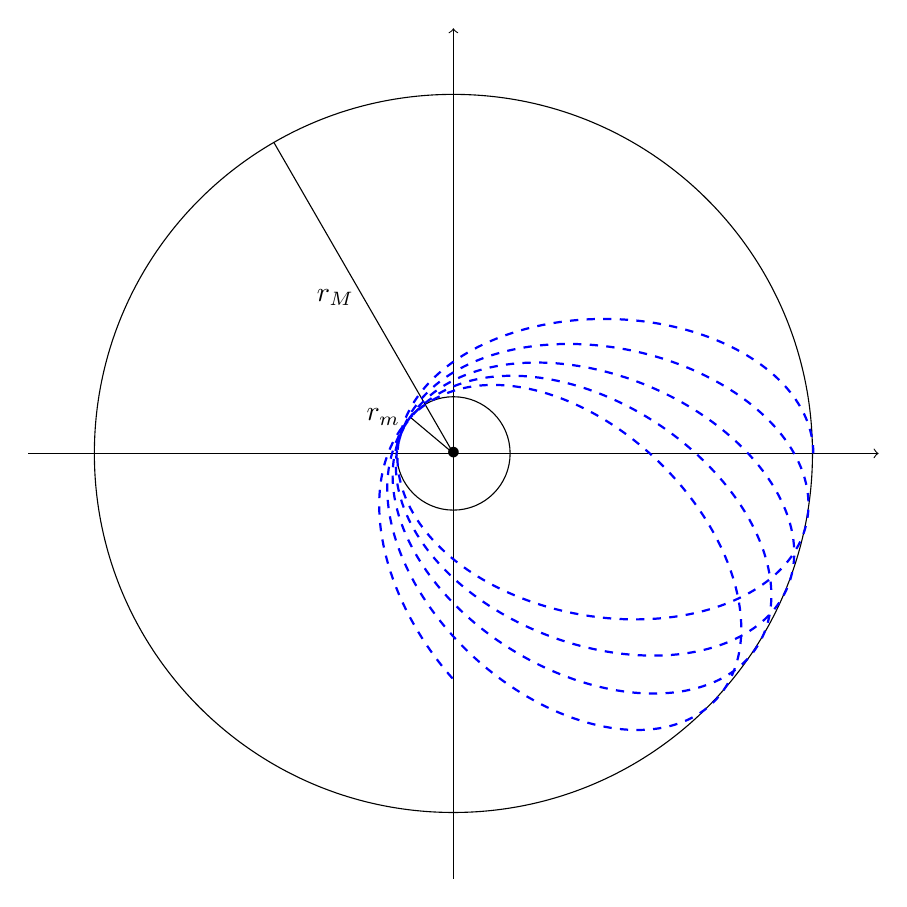
\begin{tikzpicture}[scale = 1.2]
                            \draw[->] (-4.5,0) -- (4.5,0);
                            \draw[->] (0,-4.5) -- (0,4.5);
                            \draw (0,0) circle (3.8);
                            \draw (0,0) circle (0.6);
                            \draw (0,0) node{$\bullet$};
                            %\draw[fill = black] (0,0) circle (0.3);
                            % X(t) = a*cos(t)+sqrt(a^2-b^2)
                            % Y(t) = b*sin(t)
                            \draw (0,0) -- (120:3.8) node[midway,left]{$r_M$};
                            \draw (0,0) -- (140:0.6) node[left]{$r_m$};
                            \draw[blue, dashed, thick, samples = 1000, domain=0:30] plot ({cos(deg(0.03*\x))*(2.2*cos(deg(\x))+1.6093)+sin(deg(0.03*\x))*(1.5*sin(deg(\x)))}, {-sin(deg(0.03*\x))*(2.2*cos(deg(\x))+1.6093)+cos(deg(0.03*\x))*(1.5*sin(deg(\x)))});
                        \end{tikzpicture}
                        \caption{Avancée du périastre}
                    \end{figure}
                    
                    on peut montrer que cette avancée est donnée par
                    \begin{equation}
                        \Delta \phi = \frac{6\pi GM}{ac^2(1-e^2)}
                    \end{equation}
                    
                    Le calcul de ce résultat est le sujet de la prochaine section.
                    
                    %schéma eliott
                    
                    Comme le potentiel possède deux maximas, deux trajectoire circulaire sont possibles. Cependant, un seule correspond à un minimum et donc une seul des deux trajectoire est stable (comme dans le cas newtonnien). Le rayon minimal d'une trajectoire circulaire stable est
                    \begin{equation}
                        R = \frac{6GM}{c^2}.
                    \end{equation}
                    En effet,
                    \comp
                    
                    On peut également montrer que le périastre minimal pour une trajectoire bornée est
                    \begin{equation}
                        r_m = \frac{4GM}{c^2}.
                    \end{equation}
                    Effectivement,
                    \comp
                    
                    \item $\boldsymbol{\mathscr{E}>0}$ : on a une trajectoire de type hyperbolique 
                \end{itemize}
                \item $\boldsymbol{12\left( \frac{GM}{c^} \right)^2<L^2<16\left( \frac{GM}{c^2} \right)^2}$ : les trajectoires sont les même que précédemment mais il en existe certaine qui n'ont pas de $r_m$ (crash dans l'astre central).
                
                %schéma eliott
                
                On peut montrer que, si un particule arrive de l'infini avec une vitesse $\vv{v}$, alors elle est automatiquement happée par l'étoile si sont paramètre d'impact $a$ est tel que
                \begin{equation}
                    \frac{v}{c} <\frac{4GM}{ac^2}.
                \end{equation}
                
                \comp
                
                \item $\boldsymbol{L^2<12\left( \frac{GM}{c^2} \right)^2}$ : 
                
                %schéma eliott
                
            \end{itemize}
    
    \section{Calcul de l'avancée du périastre}
    
        Pour rappel, l'énergie
        \begin{equation}
            \mathscr{E} = \frac{1}{2}\dot{r}^2+V_{\text{eff}}(r)
        \end{equation}
        avec
        \begin{equation}
            V_{\text{eff}}(r) = \frac{1}{2}\left( 1-\frac{M}{r} \right)\frac{L^2}{r^2}-\frac{M}{r}
        \end{equation}
        est une constante du mouvement. Calculons l'évolution de l'angle $\phi$ après une période complète du mouvement radial. On peut déjà s'attendre à ce que $\Delta\phi = 2\pi$ dans le cas newtonien et $\Delta\phi>2\pi$ dans le cas de la relativité générale.\\
        
        Nous savons que, 
        \begin{equation}
            \frac{d\phi}{dr} = \frac{L}{r^2}
        \end{equation}
        ce qui permet d'exprimer $\Delta\phi$ comme
        \begin{equation}
            \Delta\phi = \int_{\text{1 période}}\frac{d\phi}{dr} = L\int_{\text{1 période}}\frac{d\tau}{r^2}.
        \end{equation}
        En utilisant l'expression de $\mathscr{E}$, on voit que
        \begin{align}
            \left( \frac{r}{\tau} \right)^2 &= 2(\mathscr{E}-V_{\text{eff}}(r))\\
            \Leftrightarrow\qquad dr &= \pm\sqrt{2\mathscr{E}-V_{\text{eff}}(r)}d\tau
        \end{align}
        et donc
        \begin{equation}
            \Delta\phi = L\int_{\text{1 période}}\frac{dr}{r^2\sqrt{2\mathscr{E}-V_{\text{eff}}(r)}} = 2L\int_{r_m}^{r_M}\frac{dr}{r^2\sqrt{2\mathscr{E}-V_{\text{eff}}(r)}}
        \end{equation}
        où $r_m$ et $r_M$ sont respectivement le périastre et l'apoastre, c'est-à-dire les racines positives de l'équation $V_{\text{eff}}(r)=\mathscr{E}$. Pour simplifier les calculs, posons $\rho=\frac{1}{r}$. Dans ce cas, $\frac{dr}{r^2} = -d\rho$ et 
        \begin{equation}
            \mathscr{E}-V_{\text{eff}}(r) = \underbrace{\mathscr{E}-\frac{1}{2}L^2\rho^2+M\rho}_{\text{Newton}}+\underbrace{\frac{1}{2}ML^2\rho^3}_{\text{perturbation}}.
        \end{equation}
        Notre stratégie pour aborder ce problème sera de considérer la terme en $\rho^3$ comme une petite perturbation au terme présent en mécanique newtonienne. Si l'on note
        \begin{align}
            \rho^{(0)}_M &\equiv \frac{1}{r^{(0)}_m}\\
            \rho^{(0)}_m &\equiv \frac{1}{r^{(0)}_M}
        \end{align}
        où $r^{(0)}_m$ et $r^{(0)}_M$ désignent respectivement le périastre et l'apoastre newtonniens, on peut réécrire
        \begin{equation}
            \mathscr{E}-V_{\text{eff}}(r) = \frac{1}{2}L^2\left( \rho-\rho^{(0)_m} \right)\left( \rho^{(0)_M}-\rho \right)+2M\rho^3.
        \end{equation}
        On obtient finalement l'intégrale suivante.
        \begin{equation}
            \Delta\phi = 2\int^{\rho_M}_{\rho_m}\frac{d\rho}{\sqrt{\left( \rho-\rho^{(0)}_m \right)\left( \rho^{(0)}_M-\rho \right)+2M\rho^3}}
        \end{equation}
        
        \subsection{Cas de Newton}
        
            Dans le cas newtonnien, le terme perturbatif est nul. L'intégrale est donc al suivante :
            \begin{equation}
                \Delta\phi = 2\int^{\rho_M}_{\rho_m}\frac{d\rho}{\sqrt{\left( \rho-\rho^{(0)}_m \right)\left( \rho^{(0)}_M-\rho \right)}}.
            \end{equation}
            Cet intégrale est bien convergente et peut être effectuée par calcul direct. Cependant, utilisons une autre approche qui, bien que plus compliquée dans ce cas-ci, pourra être ré-utilisée dans le cas de la relativité générale.\\
            
            La stratégie est de résoudre l'intégrale en utilisant le théorème des résidus sur l'intégrale complexe. Pour rappel, la fonction racine carrée est définie en analyse complexe comme
            \begin{equation}
                \sqrt{z}~\hat{=}~\sqrt{\abs{z}}~e^{\frac{i}{2}\arg(z)}
            \end{equation}
            pour tout $ł\in\mathbb{C}$ où $\arg(z)$ est la \textit{fonction argument} de $z$. L'important est que $(\sqrt{z})^2$ mais la fonction de l'argument peut être définie de différente manière. La détermination de l'argument la plus courante est d'utiliser l'angle polaire $\theta$:
            \begin{equation}
                \arg(z) = \theta = \arctan\left(\frac{\Im(z)}{\Re(z)}\right).
            \end{equation}
            c'est la \textit{détermination principale}. Cette détermination n'est pas continue. En effet, 
            \begin{equation}
                \lim\limits_{y\to0^+} \arg(x+iy) = 0 \neq 2\pi = \lim\limits_{y\to0^-} \arg(x+iy).
            \end{equation}
            La fonction argument n'est pas continue le long de la demi-droite $[0,+\infty]$ (coupure). On peut utiliser d'autre détermination de l'argument de manière déplacer et à changer la forme de cette coupure à volonté mais il n'est pas possible de ne plus en avoir. En translatant la détermination principale, on peu par exemple faire en sorte que la coupure soit $[-\infty,0]$. Nous prendrons ces cas pour la suite.
            
            %schéma eliott
            
            Revenons à la fonction racine. A cause de la discontinuité de l'argument, la fonction racine est également discontinue le long de la même coupure. Pour voir cela, prenons $z_1,z_2\in\mathbb{C}$ de sorte que $z_1$ soit au dessus de la coupure et que $z_2$ soit en dessous de la coupure. Dans cas,
            \begin{align}
                \sqrt{z_1} &= i\sqrt{\abs{z_1}}\\
                \sqrt{z_2} &= -i\sqrt{\abs{z_2}}
            \end{align}
            avec $a,b\in\mathbb{R}$ et $a<b$. Il y a donc une discontinuité de signe. Dans le cas de la racine de deux nombres complexe, on a 
            \begin{equation}
                \sqrt{(z-a)(z-b)} = \sqrt{\abs{z-a}\cdot\sqrt{\abs{z-b}}}e^{\frac{i}{2}\left( \arg(z-a)-\arg(z-b) \right)}
            \end{equation}
            Il y a donc une coupure sur $[-\infty,a]$ (provenant de la fonction $\arg(z-a)$) et une coupure sur $[-\infty,b]$ (provenant de $\arg(z-b)$). Sur la demi-droite $\{x\in\mathbb{R}|x<a\}$ il y deux discontinuités de signe et donc l'effet s'annule. La coupure restante est sur l'intervalle $[a,b]$.\\
            
            Considérons la fonction
            \begin{equation*}
                z\mapsto \frac{1}{\sqrt{\left( z-a \right)\left( z-b \right)}}.
            \end{equation*}
            Cette fonction possède deux pôle et une coupure sur $[a,b]$. Si l'on intègre cette fonction sur un chemin fermé $\gamma_1$ qui entoure la coupure, alors l'intégrale peut se diviser en deux intégrales réelles où seul le signe de l'intégrant et le sens des bornes de l'intégrale change.
            \begin{align}
                \oint_{\gamma_1}\frac{dz}{\sqrt{\left( z-a \right)\left( z-b \right)}} &= \int_a^b \frac{dx}{(-i)\sqrt{\left( x-a \right)\left( x-b \right)}}+\int_b^a -\frac{dx}{(-i)\sqrt{\left( x-a \right)\left( x-b \right)}}\\
                &= 2i\int_a^b \frac{dx}{\sqrt{\left( x-a \right)\left( x-b \right)}}\\
                &= 2\pi i
            \end{align}
            par le théorème des résidus. Le facteur $-i$ vient de la racine complexe.\\
            
            Le théorème des résidus également affirme que cette intégrale est indépendante du chemin choisit. Prenons un second chemin $\gamma_{2,R}(t) = Re^{it}$, le cercle de rayon $R>\max(a,b)$. Dans ce cas
            \begin{equation}
                \lim\limits_{R\to\infty} \oint_{\gamma_{2,R}}\frac{dz}{\sqrt{\left( z-a \right)\left( z-b \right)}} = \lim\limits_{R\to\infty}\oint_{\gamma_{2,R}}\frac{dz}{z} = 2\pi.
            \end{equation}
            
            Dans le cas de notre intégrale, $a = \rho^{(0)}_m$ et $b = \rho^{(0)}_M$. Nous obtenons alors
            \begin{align}
                \oint_{\gamma_1} \frac{1}{\sqrt{\left( z-\rho^{(0)}_m \right)\left( \rho^{(0)}_M-z \right)}}~\frac{dz}{2\pi} &= \frac{1}{2\pi i} \int^{\rho_M}_{\rho_m}\frac{1}{-i\sqrt{\left( z-\rho^{(0)}_m \right)\left( \rho^{(0)}_M-z \right)}}~dz\\
                &= \frac{1}{\pi} \int^{\rho_M}_{\rho_m}\frac{d\rho}{\sqrt{\left( \rho-\rho^{(0)}_m \right)\left( \rho^{(0)}_M-\rho \right)}}
            \end{align}
            et
            \begin{equation}
                \oint_{\gamma_2} \frac{1}{\sqrt{\left( z-\rho^{(0)}_m \right)\left( \rho^{(0)}_M-z \right)}}~\frac{dz}{2\pi} = \oint_{\gamma_2}\frac{1}{z}~\frac{dz}{2\pi} = 1.
            \end{equation}
            Or, la valeur de l'intégrale ne doit pas dépendre du chemin. Ceci permet de conclure que
            \begin{equation}
                \frac{1}{\pi} \int^{\rho_M}_{\rho_m}\frac{d\rho}{\sqrt{\left( \rho-\rho^{(0)}_m \right)\left( \rho^{(0)}_M-\rho \right)}} = 1
            \end{equation}
            et donc que
            \begin{equation}
                \Delta\phi = 2 \frac{1}{\pi} \int^{\rho_M}_{\rho_m}\frac{d\rho}{\sqrt{\left( \rho-\rho^{(0)}_m \right)\left( \rho^{(0)}_M-\rho \right)}} = 2\pi.
            \end{equation}
        
        \subsection{Cas d'Einstein}
        
            Traitons le terme $M\rho^3$ perturbativement. C'est-à-dire que l'on peut se limiter au développement au premier ordre. Pour rappel, si $\varepsilon\ll1$,
            \begin{equation}
                \frac{1}{\sqrt{1+\varepsilon}}\approx1-\frac{\varepsilon}{2}
            \end{equation}
            et donc
            \begin{align}
                \Delta\phi &= 2\int^{\rho_M}_{\rho_m}\frac{d\rho}{\sqrt{\left( \rho-\rho^{(0)}_m \right)\left( \rho^{(0)}_M-\rho \right)+2M\rho^3}}\\
                &= 2\int^{\rho_M}_{\rho_m}\frac{d\rho}{\sqrt{\left( \rho-\rho^{(0)}_m \right)\left( \rho^{(0)}_M-\rho \right)}\left( 1+\frac{2M\rho^3}{\left( \rho-\rho^{(0)}_m \right)\left( \rho^{(0)}_M-\rho \right)} \right)^{\frac{1}{2}}} \\
                &\approx 2\pi + 2\int^{\rho^{(0)}_M}_{\rho^{(0)}_m}\frac{1}{\sqrt{\left( \rho-\rho^{(0)}_m \right)\left( \rho^{(0)}_M-\rho \right)}}\frac{M\rho^2}{\left( \rho-\rho^{(0)}_m \right)\left( \rho^{(0)}_M-\rho \right)} ~d\rho
            \end{align}
            Nous obtenons une intégrale divergente. Pour résoudre cette difficulté, on écrit
            \begin{align}
                \Delta\phi &= \frac{2}{2i}\oint_{\gamma_1}\frac{dz}{\sqrt{\left( z-\rho^{(0)}_m \right)\left( z-\rho^{(0)}_M \right)}-Mz^3}\\
                &\approx 2\phi+\frac{1}{i}\frac{2}{2i}\oint_{\gamma_1}\frac{1}{\sqrt{\left( z-\rho^{(0)}_m \right)\left( z-\rho^{(0)}_M \right)}}\frac{Mz^3}{2\left( z-\rho^{(0)}_m \right)\left( z-\rho^{(0)}_M \right)}~dz\\
                &= 2\pi-\frac{i}{2}\oint_{\gamma_1}\frac{Mz^3}{\left(\left( z-\rho^{(0)}_m \right)\left( z-\rho^{(0)}_M \right)\right)^{\frac{3}{2}}}~dz
            \end{align}
            pour un chemin $\gamma_1$ contour de la coupure. Comme pour le cas newtonnien, on peu prendre un second chemin $\gamma_2$ partant à l'infini pour lequel
            \begin{equation}
                \frac{1}{\left(\left( 1-\frac{\rho^{(0)}_m}{z} \right)\left( 1-\frac{\rho^{(0)}_M}{z} \right)\right)^{\frac{3}{2}}} = 1+\frac{1}{z}(\rho^{(0)}_m+\rho^{(0)}_M)^{\frac{3}{2}}+\dots
            \end{equation}
            En égalant les deux résultats, nous obtenons
            \begin{align}
                \Delta\phi &= 2\pi-\frac{2iM}{2}(2i\pi)\frac{3}{2}(\rho^{(0)}_m+\rho^{(0)}_M)^{\frac{3}{2}}\\
                &= 2\pi+3\pi M\left( \frac{1}{r^{(0)}_m}+\frac{1}{r^{(0)}_M} \right)
            \end{align}
            Or, pour rappel,
            \begin{equation}
                r = \frac{a(1-e^2)}{1-e\cos\theta}
            \end{equation}
            donc
            \begin{align}
                r_m &= \frac{a(1-e^2)}{1+e} = a(1-e)\\
                r_M &= \frac{a(1-e^2)}{1-e} = a(1+e)
            \end{align}
            En utilisant ces expressions, on trouve que
            \begin{equation}
                \frac{1}{r^{(0)}_m}+\frac{1}{r^{(0)}_M} = \frac{1}{a}\left( \frac{1}{1+e}+\frac{1}{1-e} \right) = \frac{2}{a(1-e^2)}
            \end{equation}
            ce qui permet de réécrire l'avance du périastre comme
            \begin{equation}
                \boxed{\Delta\phi = 2\pi+\frac{6\pi GM}{ac^2(1-e^2)}}
            \end{equation}
            
        \subsection{Applications numériques}
                
            Le phénomène d'avancée du périastre prédit par la relativité générale a permis d'expliquer l'avancée du périhélie de Mercure qui, observé depuis longtemps, n'avait jamais pu être réellement expliqué. L'avancée prédite par la théorie correspond exactement à ce qui est observé. Ceci a joué un grand rôle dans l'acceptation de cette théorie dans la communauté scientifique. Dans le cas de mercure,
            \begin{align}
                a &= 57.91\cdot10^8\meter\\
                e &= 0.2056\\
                \frac{GM_{\oplus}}{c^2} &= 1.475\kilo\meter
            \end{align}
            donc, si $\Delta\phi = 2\pi+(\Delta\phi)_{\text{Einstein}}$, on trouve
            \begin{equation}
                (\Delta\phi)_{\text{Einstein}} = 0.104''/\text{tour} = 43''/\text{siècle}.
            \end{equation}
            En réalité, la non-sphéricité du soleil joue également un rôle important dans l'avance du périhélie de Mercure ($\sim 532''/\text{siècle}$) mais cet effet avait déjà pu être calculé en mécanique newtonienne.\\
            
            Un autre astre a joué un rôle important lors de la validation de la théorie : la pulsar relativiste PSR 1913+16 constitué de deux étoiles à neutrons. Dans cas-ci,
            \begin{align}
                R &= 20\kilo\meter\\
                M_1 &\approx M_2 \approx 1.4M_{\odot}\\
                T &= 7.75\text{ heures}\\
                e &= 0.62
            \end{align}
            donc
            \begin{equation}
                (\Delta\phi)_{\text{Einstein}} = 6.3\cdot10^{-5}\radian/\text{révolution} = 0.071~\radian/\text{an}.
            \end{equation}
            
    \section{Déformation du temps}
    
        Dans cette partie, nous calculerons la déformation du temps subit par une horloge atomique embarquée dans un satellite. Supposons que la trajectoire est parfaitement circulaire.\\
        
        En relativité restreinte, le temps propre de l'horloge $\tau_h$ et le temps propre sur Terre $\tau_{\text{Terre}}$ sont reliés par
        \begin{equation}
            d\tau_h = \sqrt{1-v^2}~d\tau_{\text{Terre}} < d\tau_{\text{Terre}}
        \end{equation}
        où $v$ est la vitesse du satellite. L'horloge embarque retarde par rapport à l'horloge terrestre (dilatation du temps).\\
        
        Considérons maintenant le cas avec un champ de gravitation décrit par la métrique de Schwarzschild.
        
        \begin{prop}[troisième loi de Kepler]\begin{leftbar}
            Pour une trajectoire circulaire, 
            \begin{equation}
                \frac{r^3}{T^2_S} = \frac{M}{4\pi^2}
            \end{equation}
            où $T_S$ est la période de révolution dans les coordonnées de Schwarzschild.
        \end{leftbar}\end{prop}
        
        \begin{proof}
            Pour une trajectoire circulaire : $r_m=r_M$. Le rayon est donc donné par $V_{\text{eff}}'(r) = 0$.
            \begin{align}
                V_{\text{eff}}'(r) &= 0\\
                \Leftrightarrow\qquad -\frac{L^2}{r^3}+\frac{3ML^2}{r^4}+\frac{M}{r^2} &= 0\\
                \Leftrightarrow\qquad \frac{1}{r^3}\left( -L^2\left( 1-\frac{3M}{r}\right)+Mr \right) &= 0 \\
                \Leftrightarrow\qquad L^2 = \frac{Mr}{1-\frac{3M}{r}}\label{eq:L}
            \end{align}
            De plus, 
            \begin{equation}
                \frac{d\phi}{dt} = \frac{d\phi}{d\tau}\frac{d\tau}{dt} = \frac{\dot{\phi}}{\dot{t}} = \frac{L}{r^2}\frac{1}{\dot{t}}.
            \end{equation}
            Pour une trajectoire circulaire et la métrique de Schwarzschild, nous avons
            \begin{equation}
                d\tau^2 = \left( 1-\frac{2M}{r} \right)dt^2-r^2 d\phi^2.
            \end{equation}
            En utilisant la relation précédente, 
            \begin{alignat}{3}
                && d\tau^2 &= \left( 1-\frac{2M}{r} \right)dt^2-r^2 d\phi^2\\
                \Leftrightarrow&& \left(\frac{d\tau}{dt}\right)^2 &= \left( 1-\frac{2M}{r} \right)dt^2-r^2 \left(\frac{d\phi}{dt}\right)^2 \\
                \Leftrightarrow&& \frac{1}{\dot{t}^2} &= \left( 1-\frac{2M}{r} \right)-r^2\left(\frac{d\phi}{dt}\right)^2\\
                \Leftrightarrow&& \frac{r^4}{L^2}\left(\frac{d\phi}{dt}\right)^2 &= \left( 1-\frac{2M}{r} \right)-r^2\left(\frac{d\phi}{dt}\right)^2\\
                \Leftrightarrow&&~~ \left( \frac{r^4}{L^2} + r^2 \right)\left(\frac{d\phi}{dt}\right)^2 &= \left( 1-\frac{2M}{r} \right)\\
                \Leftrightarrow&& \left(\frac{d\phi}{dt}\right)^2 &= \left( 1-\frac{2M}{r} \right) \left( \frac{r^4}{L^2} + r^2 \right)^{-1}\label{eq:findevphit}
            \end{alignat}
            D'après la relation \ref{eq:L}, 
            \begin{equation}
                \frac{r^4}{L^2}+r^2 = \frac{r^4}{Mr}\left( 1-\frac{3M}{r} \right)+r^2 = \frac{r^3}{M}\left( 1-\frac{2M}{r} \right).
            \end{equation}
            En substituant dans l'équation \ref{eq:findevphit}, nous trouvons 
            \begin{equation}
                \left(\frac{d\phi}{dt}\right)^2 = \frac{1-\frac{2M}{r}}{1-\frac{2M}{r}}\frac{M}{r^3} = \frac{M}{r^3}
            \end{equation}
            donc
            \begin{equation}
                \frac{d\phi}{dt} = \frac{M}{r^{\frac{3}{2}}}.
            \end{equation}
            C'est la même relation qu'en mécanique newtonienne. On peut alors intégrer de $a$ à $T_S$, où $T_S$ est la période de révolution dans le temps de Schwarzschild (différent du temps physique).
            \begin{align}
                \int_0^{T_S}\frac{d\phi}{dt}~dt &= \int_0^{T_S}\frac{M}{r^{\frac{3}{2}}}~dt \\
                \Leftrightarrow\qquad 2\pi &= \frac{M}{r^{\frac{3}{2}}}T_S
            \end{align}
        \end{proof}
        
        La relation entre le temps propre $\tau_E$ d'un émetteur en orbite et la temps propre du récepteur $\tau_R$ sur la Terre est donnée par
        \begin{equation}
            d\tau^2_E = \left( 1-\frac{2M}{R} \right)~dt^2_E-R^2~d\phi^2
        \end{equation}
        en négligeant la rotation de la Terre. En utilisant la relation
        \begin{equation}
            d\phi^2 = \frac{M}{R^3}~dt^2_E
        \end{equation}
        qui a été utilisée dans la démonstration de la troisième loi de Kepler, nous pouvons reformuler $d\tau_E$ comme
        \begin{align}
            d\tau^2_E &= \left( 1-\frac{2M}{R}-R^2\frac{M}{R^3} \right)~dt^2_E\\
            &= \left( 1-\frac{3M}{R} \right)~dt^2_E
        \end{align}
        Par définition de $\tau_R$, 
        \begin{equation}
            d\tau^2_R = \left( 1-\frac{2M}{R_\oplus} \right)~dt^2_R.
        \end{equation}
        Lorsque le champ de gravitation est statique (c'est notre cas) donc $dt_E = dt_R$. En utilisant les deux relations précédentes, on trouve donc que
        \begin{equation}
            d\tau^2_R = \left( 1-\frac{2M}{R_\oplus} \right)~dt^2_E = \frac{1-\frac{2M}{R_\oplus}}{1-\frac{3M}{R}}~d\tau^2_E
        \end{equation}
        ou encore
        \begin{equation}
            d\tau_R = \sqrt{\frac{1-\frac{2M}{R_\oplus}}{1-\frac{3M}{R}}}~d\tau_E
        \end{equation}
        Le numérateur est d'origine gravitationnelle tandis que le dénominateur proviens aussi de la relativité restreinte. On peut voir que, si l'on veut que $d\tau_E<d\tau_R$ (comme la relativité restreinte le suggère), il faut que
        \begin{align}
            1-\frac{2M}{R_\oplus} &> 1-\frac{3M}{R} \\
            \Leftrightarrow\qquad \frac{3M}{R} &> \frac{2M}{R_\oplus}\\
            \Leftrightarrow \qquad R &< \frac{3}{2}R_\oplus
        \end{align}
        Dans ce cas, appelé \textit{orbite basse}, les de la relativité restreinte dominent. Au contraire, si
        \begin{equation}
            R > \frac{3}{2}R_\oplus
        \end{equation}
        dans le cas d'un\textit{orbite haute}, ce sont les effets de la relativité générale qui dominent : $$d\tau_E>d\tau_R$$. Ce résultat est à comparer avec le décalage des fréquences que nous avons discuté plus tôt (l'effet du décalage vers le bleu du au champ de gravitation l'emporte, donc l'horloge embarquée avance).\\
        
        Les ordres de grandeur typiques des effets du champ de gravitation sur le temps sont $\sim10^{-9}$. Ceci est particulièrement pour le système de GPS par exemple. Pour repérer la position d'un émetteur sur la Terre, plusieurs GPS mesurent la distance entre leur position et celle de l'émetteur. Si $\Delta x$ est la résolution spatiale voulue sur Terre et que $L$ est une distance typique mesurée par le satellite, alors
        \begin{equation}
            \frac{\Delta x}{L}\sim\frac{2\centi\meter}{20~000\kilo\meter}\sim10^{-9}
        \end{equation}
        donc il faut tenir compte des effets du champ de gravitation. Sans cela, on ne pourrait pas atteindre de résolution inférieur à $\Delta x\sim100\meter$.
        
    \section{Trous noirs de Schwarzschild}
    
        \subsection{Introduction}
    
            On utilise les unités géométriques $G = c = 1$. Au début de ce chapitre, nous avons montré que si l'on impose la symétrique sphérique, la solution au équation d'Einstein dans le vide est la métrique de Schwarzschild
            \begin{equation}
                ds^2 = -\left( 1-\frac{2M}{r} \right)dt^2 + \left( 1-\frac{2M}{r} \right)^{-1}dr^2 + r^2d\Omega^2
            \end{equation}
            avec $d\Omega^2 = d\theta^2+\sin^2\theta d\phi^2$. Lorsque l'on considère une étoile de rayon $R$, cette métrique est bien définie dans le vide, c'est-à-dire lorsque $r>R$. Pour $r<R$, le tenseur énergie-impulsion n'est plus identiquement nul. Dans ce cas, il faudrait trouver le tenseur-impulsion qui décrit l'intérieur stellaire et résoudre à nouveau les équations d'Einstein dont le second membre est maintenant non-nul. Notons que la métrique ne dépend que de la masse $M$ de l'étoile et pas de son rayon $R$. En particulier, la métrique ne dépend pas de la densité l'étoile. Cependant, on voit que la métrique diverge lorsque $r\to2M$ donc que se passe-t-il si $R$ est assez petit pour permettre $r\leq2M$ ? 
            \begin{defn}
                Le rayon de Schwarszchild est définit comme  
                \begin{equation}
                    R_S =\frac{2GM}{c^2}.
                \end{equation}
            \end{defn}
            Dans un premier temps, on pourrait être tenter de dire que la métrique de Schwarzschild n'est définie que pour les étoiles dont le rayon est supérieur au rayon de Schwarzschild, c'est d'ailleurs le cas la plupart du temps (pour le soleil : $R_S\sim 1.5\kilo\meter$). Pour résumer :
            
            \begin{itemize}[label = \textbullet]
                \item $\boldsymbol{R>R_S}$ : lorsque $r>R$ la solution aux équations d'Einstein est la métrique de Schwarzschild et lorsque $r<R$ la métrique de Schwarzschild n'est plus valable car nous ne sommes plus dans le vide.
                \item $\boldsymbol{R<R_S}$ : lorsque $r>R_S$ la métrique de Schwarzschild semble bien définie mais diverge lorsque $r\to R_S$. Lorsque $R<r<R_S$, la métrique de Schwarzschild semble non-définie (non-physique) même si l'on se trouve quand même dans le vide. Lorsque $r<R$ la métrique de Schwarzschild n'est plus valable car nous ne somme plus dans le vide.
                \comp
            \end{itemize}
            
            Prenons la solution de Schwarzschild au sérieux pour toutes les valeurs de $r$. On se heurte à deux problèmes : la métrique est singulière en $r=2M$ et en $r=0$. Pour comprendre, cartographies en utilisant des géodésiques radiales de genre lumière. Notons que l'on peut facilement se ramener au cas des géodésiques de genre temps à partir de l'étude des géodésiques de genre lumière et que la partie de la métrique qui nous intéresse est la partie radial car c'est elle qui diverge. Pour une géodésique radiale de genre lumière,
            \begin{equation}
                0 = \left( 1-\frac{2M}{r} \right)dt^2 - \left( 1-\frac{2M}{r} \right)^{-1}dr^2
            \end{equation}
            donc
            \begin{equation}
                 dt = \pm \left( 1-\frac{2M}{r}dt^2 \right)^{-1} dr = \pm \frac{r}{r-2M}~dr = \pm\left( 1+\frac{2M}{r-2M} \right)~dr.
            \end{equation}
            Le signe décide si la géodésique est entrante ($+$) ou sortante ($-$). Pour une géodésique radial, 
            \begin{equation}
                V_{\text{eff}}(r) = \frac{1}{2}\left( 1-\frac{2M}{r} \right)\frac{L^2}{r^2} = 
            \end{equation}
            et donc
            \begin{equation}
                \mathscr{E} = \frac{1}{2}\dot{r}^2.
            \end{equation}
            Il suit que $\dot{r}$ est une constante. En intégrant l'expression de $dt$ que nous avons trouvée ci-dessus, on obtient une expression explicite de $t$.
            \begin{equation}
                t = \pm\left( r+2M\ln\left( \frac{r-2M}{2M} \right) \right) +  \text{cste}
            \end{equation}
            
            \begin{figure}[H]
            \centering
            \begin{tikzpicture}[scale = 1.2]
                \begin{axis}[axis lines = left,xlabel = $\nicefrac{r}{R_S}$, ylabel = {$t$},xmin=0, xmax=8,ymin=0, ymax=6,xtick={0,1,...,8},ytick={0,1,...,6}]
                % entrantes
                \foreach \c in {0,1,...,15}
                   \addplot [domain=1:8, samples=100, color=blue,] {-\x-ln(\x-1)+\c};
                \foreach \c in {1,2,...,6}
                   \addplot [domain=0:1, samples=100, color=blue,] {\x+ln(1-\x)+\c};
                % sortantes
                \foreach \c in {-9,-8,...,6}
                   \addplot [domain=1:8, samples=100, color=blue,dashed] {x+ln(\x-1)+\c};
                \addplot [domain=0:1, samples=100, color=blue,dashed] {-\x-ln(1-\x)};
                \foreach \c in {0,1,...,5}
                   \addplot [domain=0:1, samples=100, color=blue,dashed] {-\x-ln(1-\x)+\c};
                \end{axis}
            \end{tikzpicture}
            \caption{Géodésiques radiales de genre lumière entrantes et sortantes}
            \end{figure}
             
            \begin{defn}
                On définit la \textit{coordonnée de la tortue} comme
                \begin{equation}
                    r_*(r) ~\hat{=}~ r+2M\ln\left( \frac{r-2M}{2M} \right).
                \end{equation}
            \end{defn}
             
            En terme de la coordonnée de la tortue, la coordonnée $t$ s'exprime comme
            \begin{equation}
                 t = \pm r_*(r) + \text{cste}
            \end{equation}
             avec le signe + pour une géodésique entrante et le signe - pour une géodésique sortante.
             
            \begin{defn}
                On définit les \textit{coordonnées de genre lumière}
                \begin{align}
                    t_1 ~&\hat{=}~ t+r_*(r)-r\\
                    u_1 ~&\hat{=}~ t_1+r
                \end{align}
                pour une géodésique entrante et
                \begin{align}
                    t_2 ~&\hat{=}~ t-r_*(r)-r\\
                    u_2 ~&\hat{=}~ t_2+r
                \end{align}
                pour une géodésique sortante.
            \end{defn}
            Notons que 
            \begin{align}
                u_1 &= t-r_*(r)\\
                u_2 &= t+r_*(t)
            \end{align}
            Donc $u_1=\text{cste}$ et $u_1=\text{cste}$.\\
            

            
            Dans un premier temps, étudier les géodésiques rentrantes. On peut voir que $t\to\infty$ lorsque $r\to 2M^+$ donc pour les observateurs qui restent à $r> 2M$, la géodésique entrante ne traverse jamais $r=2M$.
            
            \begin{defn}
                La sphère de rayon $r=2M$ est appellée \textit{horizon}.
            \end{defn}
            
            % schéma eliott
            
            De manière reliée, le décalage vers le rouge à l'horizon diverge. Notons que le champ de gravitation n'est pas forcément extrêmement fort à l'horizon. Du point de vue de l'observateur à l'extérieur, le temps écoulé pour se rapprocher de $r=2M$ est exponentiellement long. Pour l'observateur qui suit la géodésique entrante $\dot{r}$ est constant donc
            \begin{equation}
                r(\lambda) = -\lambda+\text{cste}.
            \end{equation}
            Il se voit atteindre et franchir $r=2M$ en un paramètre affinne fini (ou temps un temps fini dans le cas d'une géodésique de genre temps). Dans son référentiel, la géodésique croise l'horizon.\\
            
            Utilisons les coordonnées $t$ et $u_1$ qui sont mieux adaptée aux géodésiques entrantes. Par définition, 
            \begin{align}
                du_1 &= dt+dr_*\\
                &= dt + \left( 1+\frac{2M}{r-2M} \right)~dr\\
                &= dt +\frac{r}{2M}\frac{1}{\frac{r}{2M}-1}
            \end{align}
            donc la métrique se réécrit comme
            \begin{equation}
                ds^1 = -\left( 1-\frac{2M}{r} \right)~du^2_1 + 2du_1dr+r^2d\Omega^2
            \end{equation}
            Ces coordonnées montrent qu'il n'y a aucune singularité en $r=2M$ : ce sont uniquement les coordonnées de Schwarzschild qui sont singulière en $r=2M$. C'est une singularité apparente comme pour la singularité des coordonnées polaires dans le plan (l'angle polaire n'est pas définit lorsque le rayon es nul).\\
            
            % schéma eliott
            
            On peut diviser l'espace en deux régions :
            \begin{itemize}[label = \textbullet]
                \item \textbf{région I} $(\boldsymbol{r>2M})$ :  Cette région est asymptotiquement plate. Pour un observateur extérieur, les cônes de lumières se redressent du coté du trou noir au fur et à mesure que l'on s'en approche de manière à ce que les géodésiques ne pénètrent jamais l'horizon. Pour un observateur suivant une géodésique entrante, c'est le coté opposé du cône de lumière qui devient verticale en s'approchant de $r=2M$. Si l'on franchi l'horizon en venant de la région I, on pénètre dans la région $II$. 
                \item \textbf{région II} $(\boldsymbol{r<2M})$ : Une fois l'horizon passée, les cônes de lumière continuent à se refermer ce qui implique que toutes les trajectoires vont vers les $r$ décroissants.
            \end{itemize}
            Lorsque l'on dépasse l'horizon, les deux première composantes de ma métrique de Schwarzschild changent de signe donc $r$ de vient une coordonnée temporelle $t$ devient une coordonnée spatiale. Ceci implique que le champ de gravitation n'est pas statique quand $r<2M$, la métrique n'est plus invariante par rotation. La singularité $r=0$ est dans le futur de tout les observateurs. Il est faut de dire que l'on se fait attiré très fort par la gravité au point de ne plus pouvoir sortit. L'observateur va simplement vers son futur. Ceci décrit une cosmologie inverse de \textit{Big Crunch} à savoir une compression qui a lieu partout à la fois dans le futur. C'est l'inverse d'un \textit{Big Bang}, c'est-à-dire une explosion qui a lieu partout à la fois dans le passé. De cette manière, l'intérieur d'un trou noir de Schwarzschild décrit une cosmologie inversée pour laquelle le futur de tout les observateurs et dans la singularité en $r=0$. Notons que $r=0$ n'est pas une singularité apparente comme celle en $r=2M$ pour les coordonnées de Schwarzschild. Ceci peut être vu en observant que les invariants de courbure divergent : c'est une vraie singularité au-delà de laquelle les géodésiques ne peuvent pas êtres continuées. On dit que c'est un \textit{singularité de genre espace} car elle est partout dans l'espace en un point du temps.\\
            
            % schéma de eliott
            
            Étudions maintenant les géodésiques sortantes. Pour cela, on exprime la métrique dans la coordonnées $u_2$.
            \begin{align}
                ds^2 &= -\left( 1-\frac{2M}{r} \right)(dt^2-dr^2)+r^2 d\Omega^2\\
                &= -\left( 1-\frac{2M}{r} \right)(dt-dr)(dt+dr)+r^2 d\Omega^2\\
                &= -\left( 1-\frac{2M}{r} \right)du_1\left( du_1-2\frac{dr_*}{1-\frac{2M}{r}} \right)+r^2 d\Omega^2\\
                &= -\left( 1-\frac{2M}{r} \right)du^2_1+du_1dr+r^2 d\Omega^2\\
                &= -\left( 1-\frac{2M}{r} \right)du_2\left( du_2+2\frac{dr}{1-\frac{2M}{r}} \right)+r^2 d\Omega^2\\
                &= -\left( 1-\frac{2M}{r} \right)du^2_2-2du_2dr+r^2 d\Omega^2
            \end{align}
            
            On voit que les géodésiques sortantes qui sont dans la région II croisent l'horizon en un paramètre affinne dans le passé, c'est à nouveau un problème dû au coordonnées. Les géodésiques sortantes doivent sortir d'une région $r<2M$ mais ne peuvent pas sortir de la région II car, comme nous le verrons après, il n'y a pas de géodésiques sortantes de II). Les géodésiques sortante dans la région III proviennent donc d'une région III.\\
            
            Les géodésiques sortantes de la région II ne sortent jamais réellement. 
            Les géodésiques entrantes qui sont dans la région I ne peuvent pas venir de la région II, ce ne sont pas les mêmes que les géodésiques entrantes qui viennent de la région II. Elles viennent donc d'une région IV.\\
            
            % schéma eliott
            
            D'après ce que l'on vient de voir, les trous noir de Scwarzschild rejoignent deux régions de l'espace-temps séparée, la région I/II et la région III/IV. C'est un \textit{trou de ver}. A l'autre extrémité du trou de ver, la métrique est la même mais pas les cônes de lumière, tout les géodésiques sortent : c'est un \textit{trou blanc}. L'intérieur d'un trou décrit à une cosmologie de Big Bang (et plus de Big Crunch comme pour les trous noirs). 
            
            \begin{rmk}
                Si $R<2M$, il n'y a plus de solution statique pour le champ de gravitation, la surface de l'astre suit une géodésique de genre temps et l'astre s'effondre jusqu'à donner une singularité. Dans ce cas, il n'y a pas de région III et IV et donc pas de trou de ver.
                
                % schéma eliott
                
                Les trous noir dont on parle dan cette section sont considéré comme "éternels", on doit pouvoir remonter dans le passé aussi loin que l'on veut.
            \end{rmk}
            
            On a pu voir qu'il y a deux régions différentes telles que $r<2M$ et deux régions différentes telles que $r>2M$ donc la coordonnés radiale $r$ n'est pas une bonne coordonnée. On peut montrer que n'importe quel fonction des coordonnées $u_1$ et $u_2$ préserve les propriétés importantes de ces coordonnées. Définissons un nouveau type de coordonnées qui permet d'éliminer la singularité et donc de mieux représenter les trous de ver.
            
            \begin{defn}
                Les \textit{coordonnées de Kruskal-Szekeres} sont définies comme
                \begin{align}
                    U ~&\hat{=}~ e^{\frac{u_1}{4M}}\\
                    V ~&\hat{=}~ -e^{*\frac{u_2}{4M}}
                \end{align}
            \end{defn}
            
            On peut directement voir que 
            \begin{align}
                UV &= -e^{\frac{u_1-u_2}{4M}} = -e^{\frac{r_*}{2M}}\frac{2M}{r}\frac{e^{-\frac{r}{2M}}}{1-\frac{2M}{r}}\\
                \frac{U}{V} &= -e^{\frac{u_1+u_2}{4M}} = -e^{\frac{t}{2M}}
            \end{align}
            
            et donc
            \begin{equation}
                dUdV = -\frac{du_1}{4M}\frac{du_2}{4M}UV = -\frac{du_1du_2}{32M^2}e^{-\frac{r}{2M}}\left( 1-\frac{2M}{r} \right)
            \end{equation}
            ce qui permet de réécrire la métrique dans les coordonnées de Krusal/Szekeres comme
            \begin{equation}
                ds^2 = 32M^2e^{-\frac{r}{2M}}dUdV+r^2d\Omega^2.
            \end{equation}
            Dans ces coordonnées, les lignes deviennt
            \begin{align}
                t &= \text{cste} \to \frac{U}{V} = \text{cste}\\
                r &= \text{cste} \to UV = \text{cste}
            \end{align}
            
            % schéma eliott
            
            % schéma eliott
            
        \subsection{Pont d'Einstein-Rosen}
        
            Si l'on décrit l'espace-temps au cours du temps, on voit que les deux régions de l'espace asymptotiquement plates déconnectée jusqu'à ce qu'au moment où le trou de ver s'ouvre, c'est le \textit{pont d'Einstein-Rosen}. A ce moment-là, les régions I et IV deviennent causalement connectées et un trou noir apparaît dans ces régions qui sont maintenant équivalentes (l'espace-temps devient connexe). Les régions II et III ne sont pas équivalentes (Big Bang ou Big Crunch). Ce type de trou de verre n'est pas traversable classiquement mais il existe d'autres types de trou de ver qui le sont.
        
        \subsection{Discussions plus avancées}
        
            
            
            
\end{document}


% relire la aprtie Unités du début une fois qu'on a plus avancé pour vérifier si tout est correct

% eliott : perectionner les schémas de dilatation du temps et de contraction des longueurs + un diagramme avec les deux

% rajouter la forme x' = Lambda x + a des transformationde Poincaré